%% COLOUR GRAPHS p.182,183,192,255,256,269,270,274,282,283,286,289
%% COLOUR TEXT avFiltTab10.6-p263 bch-p239
%%
%%% \nofiles command is to format Tables 10.10, 10.11, 10.12, 10.13 and 10.14 in LOT.

\documentclass[12pt]{report}

%%% See noFiles.htm in this directory.
% don't regenerate the tableofcontents, listoffigures and listoftables files
% in list of tables (LOT), tables with 4 numbers (eg. Table 10.10) do not have
% a space between them and their captions in the LOT. need to manually configure
% the .LOT file so that:
% \contentsline {table}{\numberline {10.10}{Gaus.: Area under ROC graphs for 16 bit messages}}{204} 
% becomes 
% \contentsline {table}{\numberline {10.10}{\ Gaus.: Area under ROC graphs for 16 bit messages}}{204},
% this changes Table 10.10Gaus... to Table 10.10 Gaus
% WARNING: with "\nofiles" active, cannot add new citations, they will be undefined
%%%%%%%%%%%%%%%%%%%%%%%%%%%%%%%%%%%%%%%%%%%%%%%%%%%%%%%%%%%%%%%%%%%%
%\nofiles

\usepackage{graphicx}
\usepackage[usenames]{color}
\usepackage{amsfonts}
\usepackage{amssymb}
\usepackage{fancyhdr}
\renewcommand{\baselinestretch}{1.5}

\renewcommand{\thefootnote}{\fnsymbol{footnote}}

%%%%%%%%%%%%%%%%%%%%%%%%%%%%%%%%%%%%%%%%%%%%%%%%%%%%%%%%%%%%%%%%%%%%
%  TITLEPAGE
%%%%%%%%%%%%%%%%%%%%%%%%%%%%%%%%%%%%%%%%%%%%%%%%%%%%%%%%%%%%%%%%%%%%
\title{Multiresolutional Techniques for Digital Image Filtering and Watermarking}
\author{
        Stewart Ian Fraser \\
        B.Eng. (Hons.) University of Aberdeen \\
        A thesis presented for the degree of \\
        Doctor Of Philosophy \\
        at the University of Aberdeen \\
        Engineering Department
}
\date{May 23, 2006}


\begin{document}

\maketitle

\pagenumbering{roman}

%%%%%%%%%%%%%%%%%%%%%%%%%%%%%%%%%%%%%%%%%%%%%%%%%%%%%%%%%%%%%%%%%%%%
% ABSTRACT
%%%%%%%%%%%%%%%%%%%%%%%%%%%%%%%%%%%%%%%%%%%%%%%%%%%%%%%%%%%%%%%%%%%%
\begin{abstract}
	\small
	This thesis examines the use of multiresolutional techniques 
	in two areas of digital image processing:
	denoising (speckle reduction) and watermarking.

	A speckle reduction algorithm operating in the wavelet \emph{\`a trous} 
	domain is proposed.
	This novel algorithm iteratively approaches the 
	difference between the estimated noise standard
	deviation (in an image) and the removed noise standard deviation.
	A method for ascertaining the overall performance of a filter, 
	based upon noise removal and edge preservation,
	is presented. Comparisons between the novel denoising algorithm and existing 
	denoising filters are carried out
	using test images and medical ultrasound images. 
	Results show that the novel denoising algorithm
	reduces speckle drastically whilst maintaining sharp edges.


	Two distinct areas of digital image watermarking are addressed in this thesis: 
	(1) the presentation of a novel watermarking
	system for copyright protection and 
	(2) a fair comparison of the effects of incorporating Error Correcting 
	Codes (ECC) into various watermarking systems.
	
	The newly proposed watermarking system is blind, quantization based 
	and operates in the wavelet domain.
	Tests carried out on this novel system show it to be highly robust and reliable.

	An extensive and fair study of the effects of incorporating 
	ECCs (Bose, Chaudhuri and Hocquenghem (BCH) and repetition codes)
	into various watermarking systems is carried out.
	Spatial, Discrete Cosine Transform (DCT) and wavelet based systems are tested. 
	It is shown that it is not always beneficial to add ECCs
	into a watermarking system.
	\normalsize
\end{abstract}

%%%%%%%%%%%%%%%%%%%%%%%%%%%%%%%%%%%%%%%%%%%%%%%%%%%%%%%%%%%%%%%%%%%%
% DECLARATION
%%%%%%%%%%%%%%%%%%%%%%%%%%%%%%%%%%%%%%%%%%%%%%%%%%%%%%%%%%%%%%%%%%%%
\setlength{\topskip}{3.3cm}
\noindent \huge {\bf Declaration} \normalsize \vspace{1.44cm}
\begin{tabbing}
Full name:\hspace{0.6cm}\=Stewart Ian Fraser \\
University:\>Aberdeen University, UK \\
Department:\>Engineering \\
Thesis title:\>Multiresolutional Techniques for Digital Image Filtering \\
\>and Watermarking \\
\end{tabbing}
I hereby declare that this thesis has been composed by me
and is based on work done by me and that this thesis
has not been presented for assessment in any previous
application for a degree, diploma or other similar award.
I also declare that all sources of information have been
specifically acknowledged and all quotations distinguished
by quotation marks.
\vspace{3cm}

\noindent Signature: \rule[-0.05cm]{5cm}{0.01cm} \rule{0.5cm}{0cm} Date: \rule[-0.05cm]{5cm}{0.01cm}
\newpage

%%%%%%%%%%%%%%%%%%%%%%%%%%%%%%%%%%%%%%%%%%%%%%%%%%%%%%%%%%%%%%%%%%%%
% ACKNOWLEDGEMENTS
%%%%%%%%%%%%%%%%%%%%%%%%%%%%%%%%%%%%%%%%%%%%%%%%%%%%%%%%%%%%%%%%%%%%
%\setlength{\topskip}{3.3cm}
%\noindent \huge {\bf Acknowledgements} \normalsize \vspace{1.8cm} \\
%I would like to thank Alastair Allen very much for all his help, insight and motivation
%in making this thesis possible.
%I would also like to extend my heartfelt gratitude to all my family for
%their support and encouragement during my research; particular thanks to
%my Mum and Dad for their unwavering motivation.
%Andreas and Michael, thanks for
%brightening up the office and making it an excellent environment in which to
%work.
%\newpage


%%%%%%%%%%%%%%%%%%%%%%%%%%%%%%%%%%%%%%%%%%%%%%%%%%%%%%%%%%%%%%%%%%%%
% DEDICATION
%%%%%%%%%%%%%%%%%%%%%%%%%%%%%%%%%%%%%%%%%%%%%%%%%%%%%%%%%%%%%%%%%%%%
\setlength{\topskip}{3.3cm}
\noindent \huge {\bf Dedication \& acknowledgements} \normalsize \vspace{1.8cm} \\
The number of individuals who helped, encouraged and supported me 
through the years, in one way or another, are numerous.

First and foremost, this thesis is dedicated with love and gratitude to 
my parents, whose love and continued faith in my abilities saw me through many a tough hour. 
Thank you, you never failed to come to the rescue when needed and your 
support means more to me than I could ever put into words.

I would also like to thank my Nan and my sisters, just for being themselves, 
and our dearly departed Benji, who was a constant source of love and companionship.

An enormous thank you to my supervisor Alastair Allen for his support, insight, 
encouragement and patience. 
Thank you to Andrew Fairhead for supplying ultrasound images and thanks to the
Engineering and Physical Sciences Research Council (EPSRC) for funding my studentship. 
Thanks also to Andreas and Michael for making the office an enjoyable place to work.

\newpage

%%%%%%%%%%%%%%%%%%%%%%%%%%%%%%%%%%%%%%%%%%%%%%%%%%%%%%%%%%%%%%%%%%%%
% LIST OF CONTENTS, FIGURES AND TABLES
%%%%%%%%%%%%%%%%%%%%%%%%%%%%%%%%%%%%%%%%%%%%%%%%%%%%%%%%%%%%%%%%%%%%
\setlength{\topskip}{0cm}
\renewcommand{\baselinestretch}{1}
\begin{footnotesize}
\tableofcontents
\listoffigures
\listoftables
\end{footnotesize}
\renewcommand{\baselinestretch}{1.5}

\newpage
\renewcommand{\baselinestretch}{1}
%%%%%%%%%%%%%%%%%%%%%%%%%%%%%%%%%%%%%%%%%%%%%%%%%%%%%%%%%%%%%%%%%%%%
% ABBREVIATIONS
%%%%%%%%%%%%%%%%%%%%%%%%%%%%%%%%%%%%%%%%%%%%%%%%%%%%%%%%%%%%%%%%%%%%
\setlength{\topskip}{2.6cm}
\noindent \huge {\bf Abbreviations} \normalsize \\
\begin{table}[!ht]
\footnotesize
\begin{tabular}{p{3cm}l} \\
{\bf ASCII}     & American Standard Code for Information Interchange \\
{\bf BCH}       & Bose, Chaudhuri and Hocquenghem \\
{\bf BER}       & Bit Error Rate \\
{\bf dB}        & Decibels \\
{\bf DC}        & Direct Current \\
{\bf DCorr}     & Direct Correlation \\
{\bf DCT}       & Discrete Cosine Transform \\
{\bf DVD}       & Digital Versatile Disc \\
{\bf DWT}       & Discrete Wavelet Transform \\
        & {\bf HHx} - High High pass component (for wavelet level {\bf x}, $\mbox{\bf x} \in \mathbb{N}$)\\
        & {\bf HLx} - High Low pass component (for wavelet level {\bf x, $\mbox{\bf x} \in \mathbb{N}$})\\
        & {\bf LHx} - Low High pass component (for wavelet level {\bf x, $\mbox{\bf x} \in \mathbb{N}$})\\
        & {\bf LLx} - Low Low pass component (for wavelet level {\bf x, $\mbox{\bf x} \in \mathbb{N}$}) \\
{\bf ECC}       & Error Correcting Codes \\
{\bf ECG}               & Electrocardiograph \\
{\bf ES}               & Edge Sharpness \\
{\bf FDWT}              & Forward Discrete Wavelet Transform \\
{\bf FI}              & Fidelity Index\\
{\bf FP}              & Filter Performance \\
{\bf FPGA}      & Field Programmable Gate Array \\
{\bf FT}                & Fourier Transform \\
{\bf GRI}                & Global Restoration Index\\
{\bf HH}        & See DWT \\
{\bf HL}        & See DWT \\
{\bf HVS}               & Human Visual System \\
{\bf IDWT}              & Inverse Discrete Wavelet Transform \\
{\bf IJG}       & Independent JPEG Group \\
{\bf JND}               & Just Noticeable Difference \\
{\bf JPEG}      & Joint Photographic Experts Group \\
{\bf LH}        & See DWT \\
{\bf LL}        & See DWT \\
{\bf LSB}       & Least Significant Bit \\
{\bf MAP}       & Maximum \emph{A Posteriori} \\
{\bf MMSE}      & Minimum Mean Squared Error \\
{\bf MPEG}      & Moving Picture Experts Group \\
{\bf MSB}       & Most Significant Bit \\
\end{tabular}
\end{table}
\begin{table}[!ht]
\footnotesize
\begin{tabular}{p{3cm}l} \\
{\bf MSE}       & Mean Squared Error \\
{\bf NC}        & Normalised Correlation \\
{\bf NLOOKS}    & Number of Looks \\
{\bf norm.}     & Normalised \\
{\bf $\mbox{NR}_{\mbox{e}}$}     & Noise Reduction (about an Edge)\\
{\bf $\mbox{NR}_{\mbox{h}}$}     & Noise Reduction (Homogeneous region)\\
{\bf $\mbox{P}_{\mbox{fp}}$}      & Probability of False Positive \\
{\bf PIM}       & Picture Information Measure \\
{\bf $\mbox{\emph{P}}_{\mbox{\emph{p}}}$}       & Probability of Power of detection \\
{\bf PSNR}      & Peak Signal to Noise Ratio \\
{\bf QF}        & Quality Factor \\
{\bf rep.}      & Repetition \\
{\bf ROC}       & Receiver Operating Characteristic \\
{\bf RS}        & Reed-Solomon \\
{\bf SAR}       & Synthetic Aperture Radar \\
{\bf SI}       & Smoothing Index\\
{\bf SNR}               & Signal to Noise Ratio \\
{\bf SSIS}      & Spread Spectrum Image Steganography \\
{\bf Std.}      & Standard Deviation \\
{\bf STFT}              & Short Time Fourier Transform \\
{\bf SURE}      & Stein's Unbiased Risk Estimate \\
{\bf TPE}               & Total Perceptual Error \\
{\bf WM}        & Watermark \\
{\bf WT}        & Wavelet Transform \\
{\bf WWW}       & World Wide Web \\
\end{tabular}
\end{table}

\renewcommand{\baselinestretch}{1.5}
\normalsize

\clearpage

\setlength{\topskip}{0cm}

\pagenumbering{arabic}




%%%%%%%%%%%%%%%%%%%%%%%%%%%%%%%%%%%%%%%%%%%%%%%%%%%%%%%%%%%%%%%%%
%  MAIN BODY START
%%%%%%%%%%%%%%%%%%%%%%%%%%%%%%%%%%%%%%%%%%%%%%%%%%%%%%%%%%%%%%%%%
\chapter{Introduction}
\label{ch:introAbSumComb}

The two main topics of interest in this thesis, image denoising and image watermarking, are bound together by noise.
In the first case, how an image corrupted by noise can be smoothed whilst at the same time maintaining sharp edges is studied.
In the second case, the act of embedding a noise like signal, undetectable to the human eye,
into an image in order to verify copyright ownership is studied.

\section{Digital image denoising}
Many images are corrupted by noise of some type (\emph{e.g.}, Gaussian white noise, salt and pepper noise, speckle noise, \emph{etc}.).
Of interest in this thesis is speckle noise, which is multiplicative in nature. Speckle is formed by the interference of coherent light or 
waves, and as such, is prominent in modalities such as laser holography, Synthetic Aperture Radar (SAR) imaging and ultrasonic imaging.
There are already commonly used spatial domain filters such as the Lee and median which can reduce speckle corruption within images.
More recently, filters based upon thresholding coefficients of a decimated orthogonal Wavelet Transform (WT) have been proposed~\cite{yu96, don95}. 
However, a drawback of such schemes is the introduction of artifacts in the speckle reduced image due to the shift variant nature of 
these decimated orthogonal WTs.
In order to combat these unwanted artifacts, it is possible to compute a shift invariant version of the decimated orthogonal WT.
This involves computing the WT for every shift of the input image, which is a very time consuming task. 
An alternative approach would be to use the wavelet \emph{\`a trous}. This is a very efficient, nonorthogonal and shift invariant 
WT, thus making it an excellent choice for image denoising. 
However, the techniques used to threshold the coefficients in a decimated orthogonal WT need to
be altered for use with the wavelet \emph{\`a trous}. As such, a thresholding method operating in the wavelet \emph{\`a trous}
domain which iteratively approaches the difference
between the estimated noise standard deviation and the removed noise standard deviation is proposed. 
A novel and straightforward metric for ascertaining the overall performance of a filter is also presented. Using
this novel metric and already existing image quality metrics (the Peak Signal to Noise Ratio (PSNR) and Watson metrics), 
the performance of the new filtering scheme is compared to that of 
other filters. Results show that the new filtering scheme dramatically improves upon the other filters tested in most instances. 

\section{Digital image watermarking}
Watermarking is a relatively young discipline that aims to give copyright protection to owners of music, videos, and images that are freely 
available on the World Wide Web (WWW). It is the goal of any copyright protecting watermarking algorithm to be robust 
(able to withstand malicious and non-malicious
attacks) and at the same time be imperceptible to a human viewer. This thesis concerns itself with two distinct areas of digital image
watermarking: (1) the presentation of a novel watermarking algorithm for copyright protection and (2) fairly comparing the effects of
incorporating Error Correcting Codes (ECC) within watermarking systems.

A novel, blind and wavelet based watermarking algorithm is proposed. This is a quantization based algorithm that provides copyright protection
to digital images. The motivation for this new algorithm was based upon two existing watermarking methods. The new algorithm combines and
adapts various aspects from the two existing methods. This is done is such a way that the new algorithm improves upon both of the existing
methods.

Many authors of image watermarking algorithms claim that their methods can be made more robust with the addition of ECCs. 
As such, a selection of various watermarking algorithms (spatial, Discrete Cosine Transform (DCT) and wavelet based) are tested with and without ECCs. 
Different message lengths (short and long) are used in conjunction with different levels of repetition and 
Bose, Chaudhuri and Hocquenghem (BCH) coding so that they result
in watermarks (WM) of equal length. The robustness of different message lengths can be fairly compared by setting different detector thresholds
for each message length. The different detector thresholds for different message lengths can be equated by making the resultant probabilities
of recording a false positive reading equal.

These watermarks are then inserted into various host images. The parameters for the different watermarking algorithms
are set such that the resultant watermarked images have an equal amount of visual degradation. The Watson metric, which is based upon the
Human Visual System (HVS), is used for this purpose.

The resulting watermarked images are then attacked with various image processing techniques 
(Joint Photographic Experts Group (JPEG) compression, average filtering and Gaussian noise addition)
and the effectiveness of the watermarking 
algorithms (with and without ECCs) is ascertained. 
The benchmarking tools of attack strength, Normalised Correlation (NC), visual quality and Receiver
Operating Characteristics (ROC) are used for this purpose.

Results show that it is not always beneficial to incorporate repetition and BCH coding into a watermarking scheme. It was also found that
different watermarking systems have vastly different robustness performances depending upon the smoothness/busyness of the host image used.

\section{Thesis overview}
{\bf Chapter \ref{ch:introDN}} introduces denoising of speckle corrupted images via multiresolutional
image processing techniques. This includes an overview of speckle noise, a discussion of frequency domain
transforms, a review of wavelet shrinkage denoising, an explanation of hard and soft thresholding as well as
a study of visual artifacts.
 
{\bf Chapter \ref{ch:novelAlg}} presents a novel, iterative algorithm using the \emph{\`a trous} WT for despeckling
images. This includes a study of the wavelet \emph{\`a trous} and a presentation of the novel algorithm.
{\bf Chapter \ref{ch:IQ}} overviews and discusses various metrics for ascertaining the visual
quality of digital images. {\bf Chapter \ref{ch:resConcDN}} presents results (using  metrics from {\bf Chapter \ref{ch:IQ}})
for denoising speckle corrupted images with the novel wavelet based algorithm (from {\bf Chapter \ref{ch:novelAlg}}) and
various other filters.

{\bf Chapter \ref{chapter:wmIntro}} provides a general introduction to digital watermarking.
This includes the different properties, types and applications of watermarking systems.
The contribution of this thesis to watermarking research is outlined, namely:
(1) the proposition of a novel watermarking algorithm ({\bf Chapter \ref{chapter:dugInoue}})
and (2) a detailed study of
fairly comparing watermarking systems with and without ECCs
({\bf Chapters \ref{chapter:80_320}} and {\bf \ref{chapter:BK}}).
 
In {\bf Chapter \ref{chapter:dugInoue}}, a novel watermarking algorithm is proposed that
is based upon two already existing techniques. It is shown that this novel algorithm
has advantages over both of the techniques on which it is based.

{\bf Chapter \ref{chapter:eccB4}} gives an overview of previous watermarking work
undertaken that incorporates ECCs.
In {\bf Chapter \ref{chapter:80_320}}, a fair comparison of the effects
of BCH codes upon three watermarking systems is
performed.
This work is built upon in {\bf Chapter \ref{chapter:BK}} where a
watermarking system incorporating
various levels of repetition and BCH codes is used to embed messages of length 16, 32, 63 and 148 bits.
The effects of using various combinations of repetition and BCH coding is closely
analysed.
 
{\bf Chapter \ref{ch:finalConc}} draws conclusions for: 
(1) the novel despeckling algorithm operating in the \emph{\`a trous} wavelet domain,
(2) the newly proposed watermarking algorithm and 
(3) the study of incorporating ECCs within watermarking systems.


\chapter{Multiresolutional image despeckling: An overview}
\label{ch:introDN}
In this chapter, existing methods of removing speckle noise from digital images will
be introduced. A general introduction to speckle noise is given in Section \ref{sec:speckle}.
The advantages and disadvantages of various frequency domain transforms (Fourier and wavelet) are discussed
in Section \ref{sec:fwcNP}.
An overview of wavelet shrinkage denoising is then presented in Section \ref{sec:wsd}.
Hard and soft thresholding of wavelet coefficients is reviewed in Section \ref{sec:sht}.
In Section \ref{sec:PG}, the introduction of visual artifacts following the alteration of
WT coefficients is discussed.

\section{Speckle noise}
\label{sec:speckle}

Speckle noise is a form of multiplicative noise. It therefore causes greater
degradation within bright areas of an image than it does within dark areas. 
Laser holography, remote sensing (SAR imaging) and
ultrasonic imaging are three techniques susceptible to speckle noise degradation.
The formation of speckle noise is caused by the interference of coherent light or waves
which have been scattered from an irregular surface. These surfaces may appear
smooth to the unaided human eye, but they can be regarded as rough on the scale of
optical/electromagnetic/ultrasonic wavelengths.

Figure \ref{speckleFig} shows how the formation of speckle occurs in ultrasound imaging.
The transducer in this figure
is acting as both transmitter and receiver.
The ultrasonic waves leave the transducer in phase (\emph{i.e.}~they are coherent;
rising and falling together as they move through space). 
These waves then
hit different portions of an irregular surface and are thus reflected at different angles.
Being reflected at different angles means that each wave has to travel a
different distance back to the transducer. Hence, the waves received at the transducer are out of phase 
with each other which 
causes constructive and destructive interference. This unwanted interference causes \emph{blobs} of different shape,
size and position to appear on the generated image, \emph{i.e.}, the image has been corrupted by speckle noise.

%It is worthy to note that speckle is not noise. If an ultrasonic image grabbing experiment 
%were to be performed twice under exactly the same conditions, then the resulting 
%speckle patterns on both of the grabbed images would be identical. Hence, the speckle patterns 
%are in fact conveying information about the surface texture from which the ultrasonic waves have been reflected.
%Experienced radiologists can use this speckle information to help them in their interpretation of
%medical ultrasound images and possible diagnosis of pathologies. However, to an engineer, speckle
%is often regarded as a dominant source of noise that has to be removed before further analysis of the
%image can be made.

\begin{figure}[htb]
	\begin{center}
		\includegraphics[]{tran.pstex}
		\caption{Scattering of ultrasonic waveforms from an irregular surface}
		\label{speckleFig}
	\end{center}
\end{figure}


Due to the multiplicative nature of speckle noise, it is difficult to remove it
from bright areas of an image without causing a severe amount of blurring. 
%In order to rectify this problem, it is prudent to model the speckle noise as
%additive noise \cite{yu96}. 
One way to rectify this problem is to linearly approximate the speckle noise as additive noise \cite{yu96}.
Let the speckle corrupted pixel $z_{ij}$ be expressed by:
\begin{equation}
	z_{ij} = x_{ij}v_{ij}
	\label{speckEq}
\end{equation}
where $x_{ij}$ is the clean signal and $v_{ij}$ is the noise.
Speckle has been identified as having a negative exponential 
distribution \cite{goodman75} with a mean of one and a variance of
$\sigma_{v}^{2}$. It was shown by Lee \cite{lee80} that a linear 
approximation of equation (\ref{speckEq}) can be obtained by:
\begin{equation}
	z_{ij} = \mbox{\emph{\={v}}} x_{ij} + \mbox{\emph{\={x}}} (v_{ij} - \mbox{\emph{\={v}}})
	\label{speckEqExpand}
\end{equation}
where \emph{\={v}} is the mean of \emph{v}. Since the mean of \emph{v} is one, 
it is possible to rewrite equation (\ref{speckEqExpand}) as:
\begin{equation}
	z_{ij} = x_{ij} + u_{ij}
\end{equation}
where $u_{ij} = \mbox{\emph{\={x}}}(v_{ij} - \mbox{\emph{\={v}}})$.
The additive noise term, $u_{ij}$, has a mean of zero and a standard
deviation of $\sigma_{u} = \mbox{\emph{\={x}}} \sigma_{v}$.
Thus, the speckle noise model (multiplicative) has been approximated by an additive noise model.

%A simple way to perform this procedure is to transform the image into the
%logarithmic domain (and then inverse transform it back out again after
%filtering) as described in \cite{stark,guo,cena}.
Another way to model speckle noise as additive noise is to homomorphically transform it into the logarithmic domain
\cite{stark,guo,cena}.
%The procedure for image despeckling using this process is as follows:
Using this method, speckle noise removal from a digital image can be achieved via:
(1) Image = Image + 1, (2) Logarithm(Image), (3) Filter Image, (4) Exponential(Image) and then
(5) Image = Image - 1.
After logarithmically transforming the image, the speckle noise is additive in nature, not multiplicative.
Hence, the bright areas of the image can be despeckled without an untoward amount of
blurring. After filtering in the logarithmic domain has been carried out, the
filtered image can be inverse transformed back into the original spatial domain
via the exponential operator.

Because image formats have pixel values in the range 0 to 255,
all pixels are incremented by 1 in the first step. This prevents the
logarithm of 0 (which is minus infinity) from occurring. In the final step, this
process is reversed by subtracting 1 from all pixels of the
exponentially transformed image.

Two spatial domain filters commonly used to remove speckle noise are the median and Lee filters.
These are discussed in Appendices~\ref{sec:medianFilt} and~\ref{sec:leeFilt}, respectively.
\section{Frequency domain transforms}
\label{sec:fwcNP}
Signals are generally shown in the time domain as plots of amplitude
against time. However, these do not always convey all the signal information clearly.
For example, it may be difficult to tell which frequencies are present within a signal via a
time domain analysis. In order to get a frequency representation of a signal, it is 
necessary to apply a frequency domain transform upon it.
Transforming a signal into the frequency domain will disclose more information about the 
signal by revealing its frequency make-up.

For example, consider electrocardiographs (ECG).
The normal shape of an ECG signal is well known to cardiologists, hence an ECG which deviates from this norm 
is an indication of a possible pathology. In order to correctly analyse an ECG, 
cardiologists will study both the frequency content of the signal as well as its shape
in the time domain.

Hence, obtaining frequency information about signals under analysis has very practical applications.
This section will look at three frequency domain transforms.
Firstly, the Fourier Transform (FT) will be analysed. This transform can obtain the
frequency content of a signal. Next, the Short Time Fourier Transform (STFT) will be described.
This transform was developed to overcome some of the pitfalls of the FT.
Finally, the WT will be studied. This transform can give a more enhanced 
frequency representation of a signal than is possible with the STFT
and thus explains its widespread use within the engineering community.

\subsection{The Fourier transform}
The FT is one of the most widely used frequency domain transforms utilised in all branches of engineering.
The FT is a reversible transform which was conceived by Jean-Baptiste Joseph Fourier in the early 1800s~\cite{jfprice}. 
This means that it is possible to 
take the FT of some original data (time domain) and get transformed data (frequency domain). The 
inverse FT can then be applied to this 
transformed data (frequency domain) to get an exact replica of the original data (time domain).
Mathematically, the forward FT is defined as:
\begin{equation}
	X(\omega) = \int_{-\infty}^{\infty} x(t) e^{-j\omega t} dt
\end{equation}
where $x$ is the signal, $t$ is the time and $\omega$ is the frequency (measured in radians per second). 
The inverse FT is defined as:
\begin{equation} 
	x(t)=\int_{-\infty}^{\infty} X(w) e^{j\omega t} d\omega
\end{equation} 
A drawback of the FT is that only the time domain data or the frequency domain data
is available at any given time.

This is not a problem if the signal under scrutiny is stationary (\emph{i.e.}, if the frequency content
of the signal does not change with time). By taking the FT of a stationary signal, the frequencies
that exist in the signal will be exposed. Since these frequencies exist at all times in a
stationary signal, the FT will have analysed the frequency content of the signal accurately.

However, if the signal under scrutiny is a non-stationary 
signal (in which different frequencies are present at different times), then the FT is not sufficient.
The FT will be able to tell which frequencies are present in the non-stationary signal, but it will not be able to tell
at which times these different frequencies occurred. As an example, consider a signal composed of three
different frequency components which exist at all times (signal \emph{A}) and another signal 
with the same frequency components, each of which exist at separate time intervals (signal \emph{B}).
The FT of signals \emph{A} and \emph{B} would look similar, even though these two signals look very 
different in the time domain.
An example of this was presented in \cite{robi} and is shown in Figure \ref{fig:FTstatNonStat}.

\begin{figure}[!ht]
\setlength{\abovecaptionskip}{-0.25cm}  
\begin{center}
\includegraphics[height=14cm,width=14cm]{sigs4robi.pstex}
\end{center}
\caption{(a) stationary signal, (b) FT of stationary signal, (c) non-stationary signal, (d) FT of non-stationary signal}
\label{fig:FTstatNonStat}
\setlength{\abovecaptionskip}{0cm}  
\end{figure}

Figure~\ref{fig:FTstatNonStat}(a) shows the stationary signal $x(t) = cos(2\pi5t)+cos(2\pi10t)+cos(2\pi20t)+cos(2\pi50t)$.
This stationary signal has four frequency components of 5, 10, 20 and 50 Hertz occurring at \emph{all times}.
The FT of this signal is shown in Figure~\ref{fig:FTstatNonStat}(b). This figure
has peaks at frequencies 5, 10, 20 and 50 Hertz. Thus, the frequency content of the stationary signal has been analysed correctly by the
FT.

Figure~\ref{fig:FTstatNonStat}(c) shows a signal consisting of four different frequencies (5, 10, 20 and 50 Hertz).
This is a non-stationary signal as the different frequencies occur separately at different time intervals.
Figure~\ref{fig:FTstatNonStat}(d) shows the FT of this non-stationary signal. This figure has peaks at 5, 10, 20 and 50 Hertz.
Thus, the FT has correctly picked out the major spectral components of the non-stationary signal.





In summary, the FT can tell which frequency components are present within a signal. It cannot 
tell at what time intervals these frequencies occurred. This is acceptable for stationary signals, but
it is not sufficient for the more commonly occurring non-stationary signals.
A fuller discussion of the FT and its mathematical properties can be obtained from
\cite{jfprice, sir_mk, e_c_if, c_w_the, b_b_hub}.

\subsection{The short time Fourier transform}
The STFT is different from the FT in that the signal is
split into small segments and these segments are assumed to be stationary. A window function is used 
in order to split the signal into segments. The FT is then taken for each of these segments.
Hence, the STFT gives a time-frequency representation of the signal and it should now be possible to tell 
what frequencies exist and at what times they are present. Nevertheless, this is not the case as
it is not possible to know what frequencies exist at an exact instant in time (based upon the
Heisenberg uncertainty principle~\cite{robi}). 

However, it is possible to establish what range of frequencies exist within a certain time interval.
This is now a \emph{resolution} problem. The width of the window used to split the signal (\emph{i.e.}, the
support of the window) determines the resolution of the STFT. For example, if the window length was
infinite, it would be possible to get a perfect frequency resolution but there would
be no time resolution. Using an infinite window length for the STFT 
would give exactly the same results as would be obtained by applying the FT. 
On the other hand, if a very small window was used to split the
signal, then it would be possible to obtain very good resolution in time but this would be to the detriment of the frequency resolution (which 
would become very poor).

In summary, the STFT can give a time-frequency representation of a signal, but the resolution of the analysis
is dependent upon the size of the window used to split the signal. The same size of window is used 
for analysing fine signal details as well as the underlying signal frequency (coarse information) which results in resolution 
problems.

\subsection{The wavelet transform}
The WT analyses a signal at different frequencies with different resolutions.
Every frequency is not resolved equally, as is the case with the STFT \cite{robi}.
Like the STFT, the WT is computed by multiplying a time domain signal with a windowing function
in order to split the signal into sections. The windowing function for the WT is called a wavelet.
There are two main differences between the WT and STFT:
\begin{itemize}
	\item The FT of the split signal sections is not taken for the WT.
	\item With the WT, the width of the window (\emph{i.e.}, the wavelet) is changed for every 
	frequency component that is analysed. This is the most significant feature of the
	WT.
\end{itemize}


The advantages of the WT over the STFT can be seen in Figure \ref{timeFreq}. This figure~\cite{graps} shows
the time-frequency tiles for both the (a) STFT and (b) WT.
In Figure \ref{timeFreq}(a), the same size of analysing window (square wave) was used for all frequencies 
hence making the
resolution of the analysis the same at all locations in the time-frequency plane.
This is not a useful property of the STFT as it causes resolution problems. 
It can be seen from Figure \ref{timeFreq}(b) that the analysing windows of the WT are not of constant
size. This helps to improve the resolution of the signal in the time-frequency domain.

\begin{figure}[htb]
	\begin{center}
		% NOTE:
		% timeFreq2.fig ftp'd to ara3Linux, and xfig on ara3Linux
		% used to export it to .pstex. Exporting timeFreq2.fig
		% on xfigKelvin causes the Y-labels to be horizontal
		% rather than the required vertical. but the brackets
		% on the (a) and (b) in the fig exported from ara3 xfig
		% are different from all the other brackets in the thesis
		% generated by kelvin's xfig.
		% TO BE ABLE TO DO THIS ALL ON KELVIN, YOU CAN EDIT THE
		% .PSTEX FILE MANUALLY, SET "rot -270" FOR THE Y-AXIS
		% "Frequency" TEXT. THIS THEN GIVES BRACKETS [E.G (a),(b)]
		% LIKE THE REST OF THE FIGURES IN THE THESIS - WHICH WERE ALL
		% DONE ON KELVIN. tf4.pstex has been edited manually.
		\includegraphics[height=7cm,width=13cm]{tf4.pstex}
		\caption{Time-frequency coverage of the (a) STFT and (b) WT}
		\label{timeFreq}
	\end{center}
\end{figure}


Note that each of the boxes in Figure \ref{timeFreq}(a) are of equal area and each of the boxes in Figure \ref{timeFreq}(b) are
also of equal area. This implies that each box represents an equal portion of the time-frequency 
plane. 
In the case of the STFT, the time-frequency resolutions are constant. Once the
size of the analysing window has been selected, it will remain fixed. Hence
a decision must be made whether to select a small window to obtain an analysis
of the fine features within the signal or a large window to obtain the
underlying frequency of the signal. Which window size to use will be
dependent upon the intended application; is time or frequency resolution more important?

In the case of the WT, the boxes are of different dimensions
thus indicating that different portions are being allocated to time and frequency.
At low frequencies, the lengths of the boxes are long thus indicating very poor 
time resolution. However, the heights of the boxes are small thus indicating 
very good frequency resolution. 
At high frequencies, the opposite occurs.
The lengths of the boxes becomes shorter thus indicating good time resolution
and the height of the boxes becomes greater thereby indicating poor
frequency resolution.

Thus, unlike the STFT, the WT does not need to make a compromise
between frequency resolution and time resolution when analysing a signal. Rather,
it adapts so that good frequency resolution is obtained when analysing the long-lasting, underlying frequency
content of a signal and good time resolution is obtained when analysing the short-lived, fine
details of a signal. 
This gives a much better representation of a signal in the
time-frequency domain than is possible with the STFT.

The mathematical properties and the possible applications of the WT have been extensively 
studied~\cite{b_b_hub, graps, chuiAndyWav, daub1AndyWav, daub2AndyWav, ruskaiAndyWav, mallatAndyWav}.
Below, a brief overview of these mathematical properties~\cite{meerMasters} is given in conjunction with a worked example.

For a one dimensional signal, the underlying principle of the WT is the following. A signal
is split into two components, high frequencies (using a high pass filter, $G(\omega)$) and
low frequencies (using a low pass filter, $H(\omega)$). 
These two components are then subsampled by two (\emph{i.e.}, only one sample out of every two
is kept). This subsampling operation doubles the resolution scale (as the resolution scale increases, 
the frequencies under analysis decrease).
The coefficients obtained from this process are termed wavelet coefficients.
The low frequency component can be further split into low and high frequency components, again
using $G(\omega)$ and $H(\omega)$. This process can be repeated until the signal has been completely
decomposed or for a user specified number of steps. 
Furthermore, the original signal can be reconstructed from the obtained wavelet coefficients.
This reconstruction process is called the inverse WT.

Mathematically, the forward and inverse WTs can be described as follows~\cite{meerMasters}. Let 
\begin{equation}
	H(\omega)=\sum_{k}h_{k} \cdot e^{-jwk}
\end{equation}
and
\begin{equation}
        G(\omega)=\sum_{k}g_{k} \cdot e^{-jwk}
\end{equation}
be a low pass and a high pass filter, respectively, which satisfy certain reconstruction
criteria (stated later). A signal, $F(n)$ can be decomposed recursively as
\begin{equation}
	f^{low}_{j-1}(k)=\sum_{n}h_{n-2k}f_{j}(n)
\end{equation}
and
\begin{equation}
	f^{high}_{j-1}(k)=\sum_{n}g_{n-2k}f_{j}(n)
\end{equation}
for $j=J+1, J, \ldots, J_{0}$ where $f_{J+1}(k)=F(f), k \in \mathbb{Z}$. $J+1$ is the highest resolution level index
and $J_{0}$ is the low resolution level index. The coefficients
\begin{equation}
	f^{low}_{J_{0}}(k), f^{high}_{J_{0}}(k), f^{high}_{J_{0}+1}(k), \ldots, f^{high}_{J}(k)
\end{equation}
are called the wavelet coefficients of the signal $F(n)$, where $f^{low}_{J_{0}}(k)$ is the 
lowest resolution component of $F(n)$ (the approximation) and $f^{high}_{j}(k)$ are the 
details of $F(n)$ at various frequency bands. The signal $F(n)$ can be reconstructed recursively 
from the wavelet coefficients:
\begin{equation} 
	f^{low}_{j}(n)=\sum_{k} h_{n-2k} \cdot f^{low}_{j-1}(k) + \sum_{k} g_{n-2k} \cdot f^{high}_{j-1}(k)
\end{equation}    

To ensure the above forward and inverse WT relationship, the following orthogonality
criterion on the $H(\omega)$ and $G(\omega)$ filters is required:
\begin{equation}
|H(\omega)|^{2} + |G(\omega)|^{2} = 1
\end{equation}

An example of $H(\omega)$ and $G(\omega)$ is given by
\begin{equation}
	H(\omega)=\frac{1}{2}+\frac{1}{2} e^{-j\omega}
\end{equation}
and
\begin{equation}
        G(\omega)=\frac{1}{2}-\frac{1}{2} e^{-j\omega}
\end{equation}
which is known as the Haar wavelet filter.

As an example \cite{haarExWeb} of the Haar wavelet transform, consider the discrete signal, $y_{t}$:
\begin{equation}
	(y_{0},y_{1},y_{2},y_{3}) = (5,-1,2,0)
\end{equation}
Each of these signal values are examined in pairs (left, $l$, and right, $r$). These pairs of
signal values are then decomposed into an average ($a=\frac{l+r}{2}$) and a difference ($d=l-a=a-r$).
For the signal above, the pairs of signal values are $(5,-1)$ ($l=5, r=-1, a=2, d=3$) and $(2,0)$
($l=2, r=0, a=1, d=1$).
\begin{equation}
	(5,-1)=(2,2)+(3,-3)
\end{equation}
\begin{equation}
	(2,0)=(1,1)+(1,-1)
\end{equation}
The average is the coarse component of the pair and the difference is the detail of the pair.
Next, the smooth parts of the pairs are further decomposed ($l=2, r=1, a=1.5, d=0.5$):
\begin{equation}
	(2,2,1,1)=(1.5,1.5,1.5,1.5)+(0.5,0.5,-0.5,0.5)
\end{equation}
Hence, the original signal, $y_{t}$, can be expressed as:
\begin{eqnarray}
	(5,-1,2,0) & = & 1.5(1,1,1,1)+0.5(1,1,-1,-1)+ \nonumber \\
		   &   & 3(1,-1,0,0)+1(0,0,1,-1)
\end{eqnarray}
Figure~\ref{fig:haarEx} shows these shifts and dilations of the Haar wavelet basis.
This decomposition has been presented as a linear combination of the wavelet basis functions. The resulting
WT can be written as a vector of the four amplitudes:
\begin{equation}
	\vec{Y}=(S,D,d_{1},d_{2})=(1.5,0.5,3,1)
\end{equation}
where $S$ refers to the smooth component, $D$ refers to the detail at the first level and $d_{1}$ and
$d_{2}$ refer to the detail components at the second level.

\begin{figure}[htb]
	\begin{center}
		\includegraphics[width=13cm,height=9cm]{haarEx.pstex}
		\caption{Shifts and dilations of the Haar wavelet basis, (a) smooth component, \emph{S}, 
		(b) detail at first level, \emph{D}, (c) details at second level, $d_{1}$, (d) details at
		second level, $d_{2}$}
		\label{fig:haarEx}
	\end{center}
\end{figure}


The WT for a two dimensional image can be computed by implementing
the one dimensional WT upon the rows followed by a one dimensional WT upon the columns.
This leads to a pyramidal representation of the wavelet coefficients (shown in Figure~\ref{fig:lenaWavDecomp3}).
\begin{figure}[htb]
	\centerline{ \hbox{
		\includegraphics[width=15cm,height=6.5cm]{lenaWavDecomp5.pstex}
	}}
		\caption{Pyramidal wavelet decomposition of an image; (a) description, (b) image in wavelet domain}
		\label{fig:lenaWavDecomp3}

\end{figure}
An advantageous property of WTs is that they automatically pick out the same features that human eyes do.
Wavelets recreate an image mostly by drawing edges, which is exactly what humans do when they sketch a picture. 
It has been suggested~\cite{waveletsHumanEyes} that the analogy between WTs and human vision is no accident, that human neurons
filter visual signals in a manner very similar to wavelets. This explains the widespread use of WTs within the image 
processing community.

\subsection{Summary of frequency domain transforms}
It is useful to transform a time domain signal into the frequency domain in order to clearly 
identify the frequency components present that are otherwise obscured in the time domain.
For a long time, the FT was used to do just that. However, the FT could only tell which 
frequency components existed, it could not tell at which time intervals these frequencies existed.
Hence, time-frequency representations of a signal were not possible.

In order to rectify these short-comings, the STFT was proposed. The STFT aimed to obtain
time-frequency signal representations by splitting the time domain signal into sections
via a windowing function. However, the size of this windowing function could not be changed
which meant that resolution problems arose. Large windows gave good frequency resolution 
with poor time resolution whereas small windows gave poor frequency resolution
with good time resolution. It was not possible to get good time \emph{and} frequency resolution
using a fixed size windowing function.

These problems were addressed with the introduction of the WT. The WT also
uses a windowing function to split a time domain signal into sections. However, the size
of this windowing function is flexible. Like the STFT, the WT cannot get good time and 
frequency resolution together. However, it achieves the next best thing by having good
frequency resolution with poor time resolution and poor frequency resolution with good time resolution
in the same analysis.
It does this by using large window functions to analyse the underlying frequencies of a signal
and small window functions to analyse the fine details of a signal.
This is ideal for studying signals which have high frequency components lasting short periods of
time and low frequency components existing throughout the duration of the signal, which nearly all signals have.
Hence, the WT can give a much better time-frequency representation of a signal than the STFT.


\section{Wavelet shrinkage denoising}
\label{sec:wsd}
In \cite{taswellHWW}, Taswell gives a general introduction as to why wavelets are a
useful denoising tool as well as giving an overview as to the various ways in which they
can be used in a denoising scheme. 
The reason that wavelets provide a good means to denoising is based upon the
fact that wavelet transforms concentrate signal energy into a few coefficients
whereas noise energy is spread out over many coefficients. It is this principal that 
allows the easy separation of signal energy from noise energy when thresholding
wavelet coefficients.
It is pointed out that wavelet shrinkage denoising
is not smoothing. This is because smoothing refers to removing high frequencies 
and keeping low frequencies whereas it is the goal of denoising to remove any noise 
whilst at the same time maintaining the signal, regardless of the signal's frequency content.

In \cite{taswellHWW}, two distinct denoising procedures are outlined. Assume that the observed data
$x(t)$ is given by:
\begin{equation}
	x(t) = s(t) + n(t)
\end{equation}
where $s(t)$ is the original uncorrupted signal and $n(t)$ is an additive noise signal.
The first denoising procedure is a three step process:
\begin{equation}
	y = W(x)
\end{equation}
\begin{equation}
	z = D(y,\lambda)
\end{equation}
\begin{equation}
	\hat{s} = W^{-1}(z)
\end{equation}
where $W(\cdot)$ and $W^{-1}(\cdot)$ are orthogonal forward and inverse WTs respectively,
$D(\cdot,\lambda)$ is a denoising procedure with a threshold value of $\lambda$ and $\hat{s}(t)$ is an
estimate of $s(t)$ obtained by wavelet shrinkage denoising of $x(t)$. 
Note that in this type of denoising procedure, $\lambda$ is determined based upon the number of
transform coefficients in the wavelet domain. An example of this type of denoising scheme would
be \emph{VisuShrink} \cite{donohoJohnstone} which calculates one global threshold value which is
then applied to all wavelet scales.

The second type of denoising procedure is similar to the first except that the threshold value
used in the denoising step is data adaptive:
\begin{equation}
	 y = W(x)
\end{equation}
\begin{equation}
\label{lambdaCalc}
	\lambda = d(y)
\end{equation}
\begin{equation}
	z = D(y,\lambda)
\end{equation}
\begin{equation}
	\hat{s} = W^{-1}(z)        
\end{equation}
the operator $d(\cdot)$ helps estimate the best value $\lambda$
based upon the number of transform coefficients as well as the
data itself. An example of this type of denoising procedure would be 
the level adaptive
\emph{SureShrink} \cite{donohoJohnAdapt} which determines different thresholds
for different wavelet scales.

Note that both \emph{VisuShrink} and \emph{SureShrink} are practical
schemes requiring no \emph{a priori} knowledge of the noise variance.
Both of these schemes were compared in \cite{taswellHWW} and it was 
reported that, unsurprisingly, the \emph{SureShrink} algorithm provided images
of better visual quality than was achievable with the \emph{VisuShrink} algorithm.

	
\subsection{Literature review}	
	
In \cite{sveinssonTI}, Sveinsson \emph{et al.} propose a denoising scheme using a
translation invariant WT to reduce speckle from SAR images. The
speckle noise is modelled as additive Gaussian noise by logarithmically transforming
the SAR image. 
This scheme then calculates an individual threshold value for each scale of the 
WT via a sigmoid function. The noise is estimated from the 
\emph{high/high} subband image of the finest level of the WT. Also,
no thresholding is carried upon the \emph{low/low} subband image from the coarsest 
level of the WT. It was reported that removal of noise as well as 
preservation of (most of) the structure in the original SAR image was obtained.

In \cite{sveinssonMulti}, Sveinsson \emph{et al.} introduce a SAR image denoising 
scheme using multiwavelets. Like in \cite{sveinssonTI}, the SAR image is first 
logarithmically transformed to model the speckle as additive Gaussian noise. Also,
the noise ($\sigma$) is estimated from the \emph{high/high} subband image of the finest 
wavelet scale and the \emph{low/low} subband image of the coarsest wavelet scale is not 
thresholded. Both soft and hard thresholding were considered in this paper. The thresholds ($t$)
were calculated via $t=\gamma \sigma$, where $\gamma$ is a chosen constant.
It was reported that both hard and soft thresholding were able to remove noise
while at the same time preserve most of the original structure in the SAR image.

In \cite{fukudaSAR, fukudaSAR2}, Fukuda \emph{et al.} presented a method to remove speckle from SAR images.
Speckle is removed by reducing the pixel power of detail images in wavelet subspace. 
Rather than blindly reducing the entire range of pixel values in a wavelet
level, pixels are classified adaptively via $3 \times 3$ windows in order to determine if they contribute to 
edge information or not. Each subband in a wavelet level (horizontal, vertical and diagonal)
has its own individual $3 \times 3$ window to help classify pixels. If a pixel is determined to contribute
to edge information, it is left unaltered. If a pixel is determined to contribute to speckle,
then its magnitude is reduced. Results using this algorithm show that edges were preserved, speckle
was smoothed while at the same time visually natural SAR images were maintained. Also, the performance
of this algorithm was reported to be superior to that of the Lee filter.

In \cite{kangLeeHong}, Kang \emph{et al.} present a wavelet based technique for reducing speckle from ultrasound
images. This method makes use of the fact that noise in the wavelet domain dies out quickly with
increasing scale whereas sharp edges do not fade away with increasing scale. Edges are detected via a direct
multiplication between adjacent wavelet scales and are thus distinguishable from noise which helps improve
the quality of the denoised image. It was reported that the presented algorithm had a superior performance 
when compared to the Wiener filter.

In \cite{xu94}, Xu \emph{et al}. described a spatially selective noise filtration technique. 
This algorithm utilises the fact that edges are persistent over many wavelet scales whereas noise dies away 
very rapidly, which is very similar to the method described by Kang \emph{et al.} \cite{kangLeeHong}.
This is an iterative algorithm that attempts to construct a spatial filter mask. This is achieved by direct multiplication of two adjacent
scales of the WT (say, W1(n) and W2(n)) to obtain a Direct Correlation (DCorr(n)) signal. The power of this
DCorr(n) signal is then rescaled to match W1(n). An edge is identified and stored in the spatial filter mask for all points where
$\mbox{DCorr(n)} > \mbox{W1(n)}$. These identified edge positions are set to zero (in DCorr(n) and W1(n)) and the process repeats until the power of the
unextracted data from W1(n) is within a set tolerance of some reference noise power.
This filtration technique requires an undecimated and nonorthogonal WT.
It was reported that this method was superior to the Wiener filter at removing noise.

\"{O}ktem \emph{et al.} \cite{oktemXray} presented a wavelet based technique for the denoising
and enhancement of x-ray images. The denoising stage is a preprocessing step before 
the enhancement stage and begins with normalising the image intensity values.
After this, the WT is computed for the normalised values. A threshold
value \emph{t} is selected and wavelet coefficients with magnitude greater than \emph{t} are 
left unaltered whereas coefficients with magnitude less than \emph{t} are attenuated by an 
exponentially increasing point transformation (\emph{i.e.}, a signum function) 
normalised between zero and \emph{t}. This method of thresholding is preferred over 
hard thresholding 
to prevent unwanted artifacts being introduced into the denoised image.
Soft thresholding was not used as it causes attenuation of relatively nonsignificant details
and thus conflicts with the requirements of the enhancement stage. 


In \cite{oktemFilmGrain}, a WT domain pointwise shrinkage operator for removing
film-grain type noise is given. 
The threshold and shrinkage factor are calculated from approximation coefficients of the 
WT.
Denoising is achieved by minimising the Mean Squared 
Error (MSE) between the estimated signal spectrum and the ideal signal spectrum.
It was reported that results from this new scheme outperformed results obtained from the Kuan filter.


In \cite{kivanc}, Mih\c{c}ak \emph{et al.} introduce a simple, spatially adaptive statistical model
for wavelet coefficients and then apply it to denoise images.
Maximum \emph{A Posteriori} (MAP) calculations are performed to estimate the local variance
of wavelet coefficients and then a simple Minimum Mean Squared Error (MMSE) model is applied 
to denoise localised regions of an image. It is stated that this scheme is simple in concept
and implementation, yet produces results among the best reported in the literature. 

Zhang \emph{et al.} \cite{zhangSURE} produced a new adaptive denoising scheme based on \emph{Stein's Unbiased
Risk Estimate} (SURE) and a new class of thresholding functions. These new thresholding functions have continuous
derivatives whereas the derivative of standard soft thresholding is not continuous. This method
is shown to give a better MSE performance than that of conventional wavelet shrinkage schemes.

In \cite{roySimple}, Roy \emph{et al.} presented a new and simple algorithm for the reduction of noise from a scalar
time series. A property of this algorithm is that the threshold value is identified automatically. 
The five steps involved are:
\begin{enumerate}
	\item Differentiate the noisy signal. This has the effect of moving the contribution due
	to white noise to the finer wavelet scales where unwanted features reside (whereas the wanted
	signal features lie in the coarser wavelet levels). It is argued that the size of the
	data set decides the total number of scales available thus a suitable choice can bring out
	the noisy WT features lying in the coarser scales.
	\item Forward WT.
	\item Power estimates for different dyadic scales are calculated which provides a means 
	to automatically determine which scales to set to zero (\emph{i.e.} threshold).
	\item Inverse WT.
	\item Integrate.
\end{enumerate}
It is reported that this method works well for denoising a wide range of noise strengths, even as large as 
ten percent of the signal level.

Yu \emph{et al.} \cite{yu96} describe an iterative algorithm for determining an optimal 
global threshold for hard thresholding. This method iteratively approaches the minimum of
the difference between an estimated noise standard deviation and a removed noise standard 
deviation. Speckle corrupted images formed from the replay of a laser hologram were denoised
using this algorithm, the median filter and the Lee filter. It was reported that this
algorithm gave the most superior performance.

In \cite{moulinLiu}, Moulin \emph{et al.} state that 
universal wavelet shrinkage denoising and thresholding 
can attain near ideal estimation performance in asymptotic frameworks. However, 
in practice, asymptotic analysis is not applicable for all image denoising operations
due to the complexity of real world images. It was also shown how wavelet shrinkage 
denoising and Maximum \emph{A Posteriori} (MAP) estimates in the wavelet domain are linked.
For example, it was reported that universal hard thresholding is asymptotically equivalent to
MAP estimation assuming a generalised Gaussian distribution prior (with vanishing value of the
shape parameter).
 
\subsection{Summary of wavelet shrinkage denoising}
                                                                                                               
In \cite{taswellHWW}, Taswell states: 

\begin{quote}
``It is unlikely that one particular wavelet shrinkage denoising procedure will be suitable,
no less optimal, for all practical problems. However, 
it is likely that there will be many practical problems, for which after 
appropriate experimentation, wavelet based denoising with either hard or soft thresholding proves to be the most 
effective procedure''. 
\end{quote}    

The range of wavelet shrinkage denoising procedures outlined in this section 
in conjunction with the glut of publications addressing this topic 
highlights the breadth of this research field and lends support to Taswell's statement that there will more than likely
be a wavelet shrinkage denoising procedure to meet the requirements of almost any practical problem. 
Thus it is important that new wavelet shrinkage denoising schemes continue to be forthcoming in order to
improve upon existing techniques and to help find more optimal solutions to practical problems.

\section{Hard and soft thresholding}
\label{sec:sht}
In the wavelet domain, high frequency noise (such as speckle) does not form the
main part of the coefficients. Hence, low pass filtering of the wavelet coefficients
will remove high frequency noise. Two such low pass filtering techniques are
hard thresholding and soft thresholding. Both of these thresholding methods
have positive and negative attributes.

\subsection{Hard thresholding}
Hard thresholding implements a \emph{keep or kill} policy. The magnitudes 
of all wavelet coefficients are compared to a fixed threshold value.
If the magnitude of the wavelet coefficient is less than or equal to the 
threshold value, the coefficient
is set to zero. If the magnitude of the wavelet coefficient is greater than the threshold value, then
it is left unchanged. Equation \ref{hardEq} explains this mathematically:
\begin{equation}
        \hat{w} =  \left\{ \begin{array}{r@{\quad:\quad}l} w &
                        \quad\mbox{if}\quad |w| > t \\
                        0 & \quad\mbox{otherwise}\quad
                        \end{array} \right.
	\label{hardEq}
\end{equation}	
where $\hat{w}$ is the thresholded wavelet coefficient, $w$ is the original wavelet value and
$t$ is the threshold value.

The positive attribute of hard thresholding is that it maintains sharp features (such as edges)
very well. On the other hand, its noise reducing capabilities are not as strong as soft thresholding.

Figure \ref{hardFig} gives an example of a hard thresholding scheme showing the 
wavelet coefficient values before and after thresholding (using a threshold value of 0.3).

\begin{figure}[htb]
	\begin{center}
		% edit hard2.pstex manually and set: "rot -270.0" to rotate y-axis
		\includegraphics[height=7.5cm,width=7.5cm]{hard2.pstex}
	\caption{Illustration of hard thresholding} 
	\label{hardFig}
	\end{center}
\end{figure}


\subsection{Soft thresholding}
\label{subsec:softTh}
Soft thresholding shrinks the absolute value of all wavelet coefficients towards zero.
Like hard thresholding, soft thresholding compares the magnitudes of all wavelet coefficients
to a fixed threshold value and if the magnitude of the pixel is 
less than or equal to this threshold value, it is set to zero. However, if the 
pixel magnitude is greater than the threshold value, its absolute value is shrunk 
towards zero. How much it is shrunk depends upon the threshold value.
Equation \ref{softEq} explains this mathematically:
\begin{equation}
        \hat{w} =  \left\{ \begin{array}{r@{\quad:\quad}l} \mbox{sgn}(w)(|w|-t) & \quad\mbox{if}\quad |w| > t \\
                        0 & \quad\mbox{otherwise}\quad
                        \end{array} \right.
	\label{softEq}
\end{equation}	
where $\hat{w}$ is the thresholded wavelet coefficient, $w$ is the original wavelet value and
$t$ is the threshold value.

The positive attribute of soft thresholding is its ability to remove noise very well.
It achieves this because it shrinks all wavelet coefficients towards zero (unlike hard thresholding). 
However, this global shrinking of all wavelet coefficients also causes it to blur edges 
to a greater extent than hard thresholding.

Figure \ref{softFig} gives an example of a soft thresholding scheme showing the 
wavelet coefficient values before and after thresholding (using a threshold value of 0.3).

\begin{figure}[htb]
	\begin{center}
		% edit soft2.pstex manually and set: "rot -270.0" to rotate y-axis
		\includegraphics[height=7.5cm,width=7.5cm]{soft2.pstex}
		\caption{Illustration of soft thresholding} 
		\label{softFig}
	\end{center}
\end{figure}

\subsubsection{Optimal soft thresholding calculation}
In \cite{don95}, Donoho introduced the following optimal wavelet shrinkage method:
\begin{enumerate}
	\item Apply the WT to the data to obtain \emph{N} coefficients.
	\item Set a threshold $t = \gamma \sqrt{2\mbox{log}(n)}\sigma / \sqrt{n}$, where
	$n$ is the number of data points, $\gamma$ is an experimentally derived constant 
	and $\sigma$ is the estimated
	noise level in the data.
	This threshold value is then used in the nonlinear soft thresholding scheme
	$\hat{w} = \mbox{sgn}(w)(|w|-t)_{+}$. This is done for \emph{all}
	wavelet coefficients.
	\item Apply the inverse WT to get the estimated data.
\end{enumerate}

This procedure does not exhibit any noise induced structures
and
it can maintain sharp features quite well. 

Guo \emph{et al.} \cite{guo} outlined a simple and effective procedure for estimating the noise
in the data. Using a decimated orthogonal WT, they take the finest
detail coefficients from the first level of the transform. The standard deviation of these 
coefficients are then taken as the estimate for the noise within the data.

They then proceeded to test both hard and soft thresholding schemes upon speckle corrupted images using 
Donoho's \cite{don95} threshold calculation (although optimal for soft thresholding,
it can nevertheless be used in a hard thresholding scheme too).
Firstly, they estimated the noise in the data ($\sigma$) using the finest
detail coefficients from the first level of the WT. This value
was then used to help determine which threshold value ($t$) to use: 
$t = \gamma \sqrt{2\mbox{log}(n)}\sigma / \sqrt{n}$. This threshold value was then
applied (via hard and soft thresholding) to all wavelet coefficients except the most coarse low frequency 
wavelet coefficients (in order to guarantee that the mean of the processed data is the same 
as the mean of the original data).

Using this method, they reported that for $t = 1.5\sigma \mbox{ ... } 3\sigma$
the noise in the image was suppressed by $86.6\% \mbox{ ... } 99.7\%$. Also,
they reported that soft thresholding is more adept at removing noise than hard thresholding 
whereas hard thresholding preserves sharp features better than soft thresholding.

\section{Visual artifacts}
\label{sec:PG}
\subsection{Perfect reconstruction}
\label{perfectReconstruction}
Perfect reconstruction is achievable when using a decimated
orthogonal WT. However, this is based upon the assumption 
that the wavelet coefficients are left unaltered. Hence, taking 
a two dimensional decimated orthogonal WT of an image
(say, image \emph{X}) to obtain a set of wavelet coefficients and then applying 
the inverse
transform to these unaltered coefficients will yield 
an identical copy of image \emph{X}. 
This copy will not suffer from any transform induced artifacts. 
Figure \ref{dwtProcess} outlines this process, where the orthogonal and 
decimated Forward Discrete Wavelet Transform (FDWT) and Inverse Discrete Wavelet Transform (IDWT)
are being used.
A more comprehensive explaination of wavelet transforms (including orthogonal and biorthogonal basis,
frames and perfect reconstruction)
can be found in~\cite{mallatAndyWav}.
\vspace{0.4cm}
\begin{figure}[htb]
	\begin{center}
	\includegraphics[height=2cm,width=10cm]{dwtProcess2.pstex}
	\caption{Perfect reconstruction using the WT} 
	\label{dwtProcess}
	\end{center}
\end{figure}

\subsection{Pseudo-Gibbs phenomena}
\label{pseudoGibbsSection}
If the wavelet coefficients of a decimated orthogonal WT are altered
before the application of the inverse transform (\emph{e.g.}, thresholded), visual artifacts would be introduced into the 
reconstructed image. Figure \ref{dwtProcessFlawed} outlines this scenario.
\vspace{0.4cm}
\begin{figure}[htb]
	\begin{center}
        \includegraphics[height=2cm,width=10cm]{dwtProcessFlawed2.pstex}
	\caption{Introducing visual artifacts using the WT}
        \label{dwtProcessFlawed}
	\end{center}
\end{figure}

The production of such artifacts also arises when the FT is used rather than the decimated 
orthogonal WT. In the Fourier case, the artifacts are global in nature and are termed Gibbs phenomena.
In the wavelet case, the artifacts are smaller and more localised than those produced with the FT and are
thus termed pseudo-Gibbs phenomena \cite{durand}.

The Pseudo-Gibbs phenomenon occurs in the neighbourhood of discontinuities in the signal/image and exhibits itself as
alternating undershoot and overshoot \cite{coifman}.
This phenomenon is the direct result of the alignment between the wavelet basis functions and the discontinuities in the
signal/image.
After the wavelet coefficients have been altered (\emph{e.g.}, thresholded), then the wavelet basis functions and the 
altered wavelet coefficients are no longer perfectly aligned.

This misalignment may or may not result in the introduction of visual artifacts in the reconstructed image.
If the discontinuity in the signal/image occurs at the same location as a discontinuity in the wavelet basis
functions, then no visual artifact will be introduced into the reconstructed signal/image. However, if the discontinuities
in the signal/image and the basis function are not aligned, then the size of the introduced visual artifact 
will be proportional to the amount of misalignment \cite{coifman}. 

As an example, consider a signal with \emph{n}
samples and the Haar wavelet (which has a discontinuity at $n/2$). If a discontinuity is present at $n/2$ in the signal, then 
no pseudo-Gibbs phenomena will occur. If the discontinuity in the signal occurs at $n/3$, then a significant amount of
pseudo-Gibbs phenomena will occur.

\subsubsection{Cycle spinning}
In order to combat the pseudo-Gibbs phenomenon that results from thresholding the
coefficients from a decimated orthogonal WT, cycle spinning
has been proposed by Coifman \emph{et al.} \cite{coifman}. This method has also been used by Cena \emph{et al.}
\cite {cena} to denoise medical ultrasound images.

The idea of cycle spinning is to threshold the wavelet coefficients from all possible shifts 
of the input signal/image. By shifting the input signal/image, it is hoped that the misalignment 
between the thresholded coefficients and the wavelet basis will be neutralized. Once all possible
shifts of the input signal/image have been thresholded, the results are then averaged to minimize
pseudo-Gibbs phenomena. This process is outlined in Figure \ref{CSprocess}.
\vspace{0.4cm}
\begin{figure}[htb]
	\begin{center}
		\includegraphics[height=2cm,width=10cm]{CSprocess2.pstex}
		\caption{Cycle spinning process for thresholding wavelet coefficients}
		\label{CSprocess}
	\end{center}
\end{figure}
The constant \emph{shifting-thresholding-unshifting} has the effect of making the transform stationary,
\emph{i.e.}, it is now shift-invariant.

The best results are obtained when all possible shifts of the input signal/image are computed,
however, this requires a lot of computational time to calculate. 
The decimated orthogonal WT has a computational complexity of $O(n)$ whereas the
translation invariant version (where all shifts of the input signal/image are accounted for)
has a computational complexity of $O(n\mbox{log}_{2}n)$ \cite{cena, coifman, lang96}.

In order to reduce the computational time,
a range of shifts for the input signal/image can be calculated instead. This will reduce the pseudo-Gibbs 
phenomena associated with thresholding, but not to the same extent as 
would have been possible by calculating all possible shifts.
This is due to the fact that nearly all signals/images contain many discontinuities and the best shift for one discontinuity
may not necessarily be the best shift for other discontinuities.

Figure \ref{signalExample}(a) shows a test signal and Figure \ref{signalExample}(b) shows the same
signal with additive Gaussian noise ($\sigma_{norm.}^{2} = 0.0025$)\footnote{Gaussian noise with 
normalised variance of 0.0025}.
Figure \ref{signalExample}(c) shows the overshooting and undershooting about the discontinuity that is
pseudo-Gibbs phenomena. This signal has been hard thresholded with a value of 0.2 via a decimated orthogonal
WT (using a length 6 Symmlet basis function).
The coefficient magnitudes about the edge can be seen to swing wildly as the alignment between the 
edge and the wavelet basis functions change (even a one sample misalignment can incite pseudo-Gibbs phenomena \cite{choi}).
Figure \ref{signalExample}(d) shows the same noisy signal thresholded with identical parameters as Figure \ref{signalExample}(c) 
but with cycle spinning for all shifts. Note that the amount of overshooting and undershooting 
about the edge has been dramatically reduced. 
\begin{figure}[htb]
	\begin{center}
	\includegraphics[height=10cm,width=13cm]{spin4figs.pstex}
	\caption{Denoising a signal with and without cycle spinning}
	\label{signalExample}
	\end{center}
\end{figure}



\subsection{Visual artifacts from wavelet denoising}
The idea behind wavelet denoising is to concentrate the signal/image energy into a few main coefficients
whilst the noise energy is distributed more evenly over all the coefficients \cite{kings}.
By suppressing the magnitudes of the lower energy coefficients, the noise is attenuated much more than the
signal hence improving the Signal to Noise Ratio (SNR). 

When suppressing the magnitudes of wavelet coefficients, some subtle problems \cite{choi} can arise.
These are: (1) pseudo-Gibbs phenomena, (2) edge blurring and (3) wavelet shaped ripples in smooth regions.
Pseudo-Gibbs phenomena have been discussed in Section \ref{pseudoGibbsSection}.
The noise in a corrupted signal/image can cause large coefficients from edge regions 
to become small, and removing them (via thresholding) causes the edge regions to become blurred
in the restored signal/image.
Alternatively, the noise in a corrupted signal/image can cause small coefficients from a 
homogeneous area to become large and retaining them (after thresholding) produces wavelet shaped
ripples in the restored signal/image.

The Lena images in Figure \ref{badDenoising} highlight these problems.
Figure \ref{badDenoising}(a) shows the original uncorrupted Lena image and
Figure \ref{badDenoising}(b) shows the Lena image corrupted with speckle noise.
In the hard thresholded image, Figure \ref{badDenoising}(c), wavelet shaped ripples are apparent in the smooth
regions. In the soft thresholded image, Figure \ref{badDenoising}(d), 
the edges can be seen to have been blurred when compared to
the original image.

\begin{figure}[htb]
	\centerline{ \hbox {
	\includegraphics[height=15cm,width=15cm]{l_all4.pstex}
	}}
	\caption{(a) original image, (b) speckle corrupted image, (c) hard thresholded image, (d) soft thresholded image}
	\label{badDenoising}
\end{figure}

\section{Summary}
This chapter has given an overview of multiresolutional image despeckling, with an emphasis
on wavelet shrinkage denoising. 

Problems arising from wavelet shrinkage denoising using the decimated orthogonal WT have been
highlighted, \emph{e.g.}, pseudo-Gibbs phenomena (Section~\ref{sec:PG}), which may be attributed to the shift 
variant nature of this transform.

Cycle spinning is a method which can alter the decimated orthogonal WT from shift variant to shift invariant 
(thus minimising pseudo-Gibbs phenomena). However, cycle spinning increases the computational complexity of this transform from 
$O(n)$ to $O(n\mbox{log}_{2}n)$.

In Chapter~\ref{ch:novelAlg}, the wavelet \emph{\`a trous} will be introduced.
This WT is shift invariant yet has a low computational complexity of $O(n)$. A novel despeckling
algorithm using this WT will be presented.
\chapter{A novel denoising algorithm using the \emph{\`a trous} WT}
\label{ch:novelAlg}
This chapter presents a novel algorithm operating upon the coefficients
obtained from the wavelet \emph{\`a trous}. Section \ref{sec:WAT} introduces the 
\emph{\`a trous} WT and Section \ref{sec:novelAlg} details the novel denoising algorithm.


\section{The \emph{\`a trous} WT} 
\label{sec:WAT}

The \emph{\`a trous} WT is a nonorthogonal, redundant (stationary) and shift invariant transform~\cite{stark}.
The \emph{\`a trous} WT does not subsample a signal/image; it is redundant. 
The computational complexity of the \emph{\`a trous} WT is $O(n)$~\cite{morehart}.

The dimensions of the input 
data to the \emph{\`a trous} WT can be of any size, they do not need to be integer powers of two (dyadic length), as is
required by the decimated orthogonal WT. 
The noise terms in an orthogonal WT are not correlated, whereas the noise terms in a nonorthogonal WT are correlated~\cite{cena, lang96}.
Thus, a denoising algorithm designed to operate within a decimated orthogonal WT domain would not function in the
wavelet \emph{\`a trous} domain (as outlined in Section~\ref{sec:novelAlg}, where a denoising algorithm designed to operate
in a decimated orthogonal wavelet domain is adapted to operate in the wavelet \emph{\`a trous} domain).
Table~\ref{tab:wavComp} compares the characteristics of the decimated orthogonal WT, 
the cycle spun decimated orthogonal WT (Section~\ref{pseudoGibbsSection}) and the \emph{\`a trous} WT. It can be seen that 
the wavelet \emph{\`a trous} provides shift invariance with a low level of computational complexity.

\begin{table}[ht]
\begin{center}
\begin{scriptsize}
\begin{tabular}{|c|c|c|c|} \hline
			& decimated 			& decimated 		 		& undecimated 	 	\\ 
			& orthogonal 			& orthogonal 				& \emph{\`a trous}  	\\ 
			& WT				& WT (cycle spun)			& WT 			\\ \hline
variant/invariant	& shift variant			& shift invariant			& shift invariant  	\\ \hline
complexity		& $O(n)$			& $O(n\mbox{log}_{2}n$)			& $O(n)$		\\ \hline
input data dimensions	& integer power of two		& integer power of two			& any			\\ \hline
noise terms		& uncorrelated			& uncorrelated				& correlated		\\ \hline
\end{tabular}
\end{scriptsize}
\caption{Comparison of three different wavelet transforms}
\label{tab:wavComp}
\end{center}
\end{table}	

Sections~\ref{sec:fwd1dAT}, \ref{sec:inv1dAT} and \ref{sec:fwdinv2dAT} outline
the procedures required to compute the wavelet \emph{\`a trous}.
A more detailed mathematical description of these procedures can be found in
\cite{stark, holdschneider89, stark95, shensa1992}.

\subsection{The forward 1-d {\em \`a trous} WT}
\label{sec:fwd1dAT}
In order to implement the \emph{\`a trous} WT, a scaling function
with low pass filtering characteristics must first be selected. This
scaling function may be, for example, a linear scaling function or a
spline scaling function. 
Equation (\ref{linEq}) is an example of a discrete linear scaling function:
\begin{equation}
        c_{j+1}(k)=\frac{1}{4}c_{j}(k-2^{j})+\frac{1}{2}c_{j}(k)+
        \frac{1}{4}c_{j}(k+2^{j})
	\label{linEq}
\end{equation}
and equation (\ref{splineEq}) is an example of a $\mbox{B}_{3}$-spline
scaling function:
\begin{equation}
        c_{j+1}(k) = \frac{1}{16}c_{j}(k-2^{j+1})+\frac{1}{4}c_{j}(k-2^{j})+
                        \frac{3}{8}c_{j}(k)+
			\frac{1}{4}c_{j}(k+2^{j})+
                        \frac{1}{16}c_{j}(k+2^{j+1})
	\label{splineEq}
\end{equation}
Equations (\ref{linEq}) and (\ref{splineEq}) show how the smoothed data $c_{j}(k)$
at resolution $j$ and position $k$ can be obtained from the original
sampled data $c_{0}(k)$.

It can be seen from equations (\ref{linEq}) and (\ref{splineEq}) that the sampling distance is dependent 
upon $j$, the scale level.
As the scale level increases, the approximation level becomes ever more
coarse ({\em i.e.,} more average). 
In order to achieve this, the sampling distance is increased by a factor of two
from one level to the next (as opposed to downsampling the signal as is the case
with the decimated orthogonal WT). This process is 
outlined in Figure \ref{at_dots}. Note that this is where the name \emph{\`a trous}
(with holes) WT originates from; there are \emph{holes} between samples.
\begin{figure}[htb]
        \begin{center}
                \includegraphics[width=13cm]{at_dots.pstex}
		\caption{Example of a linear scaling function}
	\label{at_dots}
        \end{center}
\end{figure}

Once the set of scale levels $C_{0}, C_{1}, \mbox{...}, C_{p}$ have been obtained, calculation
of the corresponding wavelet levels is a straightforward process. 
The wavelet level at resolution $j$, 
$w_{j}$, can be
found from
the \emph{difference} between adjacent approximation levels:
\begin{equation}
        w_{j}(k)=c_{j-1}(k)-c_{j}(k)
\end{equation}

\subsection{The inverse 1-d {\em \`a trous} WT}
\label{sec:inv1dAT}
Reconstruction of the original input signal can be found by
adding all the wavelet levels $w_{j}(k)$ to the final smoothed signal:
\begin{equation}
	\label{reconEq}
        c_{0}(k)=c_{p}(k)+\sum_{j=1}^{p}w_{j}(k)
\end{equation}
where $c_{p}$ is the final approximation level (residual signal) and $p$ is the number of wavelet levels.

\subsection{The forward and inverse 2-d  {\em \`a trous} WT}
\label{sec:fwdinv2dAT}
The scaling algorithm can be extended to the two dimensional case by performing
a row by row convolution directly followed by a column by column convolution.
Alternatively, a sliding window can be used whose coefficients can be from a linear scaling function:
\begin{equation}
	\left( 	\frac{1}{4} \mbox{ } \frac{1}{2} \mbox{ } \frac{1}{4} \right) 
	\otimes 
	\left(	\begin{array}{c}
			1/4 \\
			1/2 \\
			1/4
		\end{array}
	\right)
	\label{linMask}
\end{equation}
or, alternatively, from a spline scaling function ($\mbox{B}_{3}$-spline in this case):
\begin{equation}
	\left(  \frac{1}{16} \mbox{ } \frac{1}{4} \mbox{ } \frac{3}{8} \mbox{ } \frac{1}{4} \mbox{ } \frac{1}{16} \right)
	\otimes
	\left(  \begin{array}{c}
			1/16 \\
			1/4  \\
			3/8  \\
			1/4  \\
			1/16 \\
		\end{array}
	\label{splineMask}
	\right)
\end{equation}
where $\otimes$ is the Kronecker product. 

Figure~\ref{atrousEg} shows an original input image (Lena) and three scaled images obtained
by applying a linear scaling function (equation (\ref{linMask})). 
The normalised absolute values of the wavelet levels are shown for greater clarity.
Note that these images have 
not been downsampled and that the analysis becomes more coarse (average) as the scale increases.
The final scaled image (most coarse) is termed the \emph{residual} image.
Calculation of the associated wavelet images is simply a process of finding the difference
between adjacent scaled images.
All the scaled images, apart from the residual image, are no longer required after calculation
of the wavelet levels. 
\begin{figure}[!ht]
        \begin{center}
                \includegraphics[height=16cm,width=9cm]{atrousEg.pstex}
        \end{center}
        \caption{The forward 2-d \emph{\`a trous} WT}
        \label{atrousEg}
\end{figure}

The inverse 2-d \emph{\`a trous} WT is shown in Figure \ref{atrousInvEg}. This process
is the same as the 1-d case (equation (\ref{reconEq})) in that all the wavelet levels are added to the residual image in 
order to obtain a perfect reconstruction of the input image (assuming no alteration to either the residual or wavelet 
images has occurred).
\begin{figure}[htb]
        \begin{center}
                \includegraphics[height=3cm,width=13cm]{atrousInvEg.pstex}
		\caption{The inverse 2-d \emph{\`a trous} WT}
		\label{atrousInvEg}		
        \end{center}
\end{figure}

The following pseudo-code shows the process for calculating the forward and 
inverse \emph{\`a trous} WT. 
This code computes three wavelet levels (\tt \footnotesize w0, w1 \normalsize \rm and \tt \footnotesize w2\normalsize \rm).

\noindent
\begin{minipage}[t]{15cm}
\renewcommand{\baselinestretch}{1}
\footnotesize
\begin{verbatim}
% Reading input image to be analysed.	
imageIn=imread(`lena.jpg');	

% Apply linear scaling via sliding mask. 
s0=linScaling(imageIn,0); 	
s1=linScaling(s0,1);		
residualImg=linScaling(s1,2);	

% Obtain wavelet levels.
w0=imageIn-s0;	
w1=s0-s1;	
w2=s1-s2;	

% Can perform operations (denoising, edge detection, ... etc.)	
% on wavelet images at this point, but not done here in order	
% to achieve perfect reconstruction of input image.		

% Inverse transform.	
reconstructedImg=residualImg+w2+w1+w0;	
\end{verbatim}		
\normalsize		
\end{minipage}	% end minipage so verbatim text not split between pages
\renewcommand{\baselinestretch}{1.5}

\vspace{0.5cm}
\par
The \tt \footnotesize linScaling() \normalsize \rm function takes two parameters, the image to be linearly 
scaled and the resolution for the analysis (which refers to the distance between samples, see Figure \ref{slideWin}).
The first application of this function has a resolution of 0,
and from equation (\ref{linEq}), it can be seen that setting $j$ (the resolution parameter) to 0 will render 
the distance between samples to be 1 ($2^{0} = 1$); this can be seen in Figure \ref{slideWin}(a).
Upon the second application of the  \tt \footnotesize linScaling() \normalsize \rm function,
the distance between samples will be 2 ($2^{1} = 2$); this can be seen in Figure \ref{slideWin}(b).
Finally, the third application of the \tt \footnotesize linScaling() \normalsize \rm function
will result in a distance between samples of 4 ($2^{2} = 4$);
this can be seen in Figure \ref{slideWin}(c).

The first scaled image (low pass filtered) is obtained by applying the \tt \footnotesize linScaling() \normalsize \rm function
(distance between samples of 1) to the original input image to get \tt \footnotesize s0\normalsize \rm.
The next scaled image \tt \footnotesize s1 \normalsize \rm is obtained by applying the 
\tt \footnotesize linScaling() \normalsize \rm function (distance between samples of 2) to 
\tt \footnotesize s0\normalsize \rm. Thus, \tt \footnotesize s1 \normalsize \rm is a coarse approximation 
of \tt \footnotesize s0\normalsize \rm. Finally, \tt \footnotesize s2 \normalsize \rm is obtained by applying
the \tt \footnotesize linScaling() \normalsize \rm function to \tt \footnotesize s1 \normalsize \rm (distance
between samples of 4), thus, \tt \footnotesize s2 \normalsize \rm is a coarse approximation of
\tt \footnotesize s1\normalsize \rm.


The residual image is a very rough approximation of the input image (obtained by repeated low pass filtering).
The original input image can be reconstructed by adding the three wavelet levels
(\tt \footnotesize w0\normalsize \rm,
\tt \footnotesize w1 \normalsize \rm and
\tt \footnotesize w2\normalsize \rm)
to the residual image.
The first wavelet level, \tt \footnotesize w0\normalsize \rm, contains the high frequency information (the fine details within the image).
The second wavelet level, \tt \footnotesize w1\normalsize \rm, contains the mid frequency information.
The third wavelet level, \tt \footnotesize w2\normalsize \rm, contains the low frequency information.

\begin{figure}[!ht]
        \begin{center}
                \includegraphics[height=6cm,width=13cm]{slideWin2.pstex}
		\caption{Different resolutions for the 2-d linear scaling function; (a) first level, 
		(b) second level, (c) third level}
		\label{slideWin}
        \end{center}
\end{figure}



\section{A novel denoising algorithm}
\label{sec:novelAlg}

This novel denoising algorithm was inspired by Yu \emph{et al.} \cite{yu96} which itself was inspired jointly by 
Donoho \cite{don95} and Guo \emph{et al.} \cite{guo}.

In \cite{don95}, Donoho presented a method for optimally recovering functions
from data corrupted with Gaussian noise; this was termed soft thresholding. Donoho's threshold calculation
could also be used in a hard thresholding scheme, but then the calculated threshold value would no longer be optimal. 

In \cite{guo}, Guo \emph{et al.} compared soft and hard thresholding schemes upon SAR images and reported that hard thresholding 
can maintain fine features to a greater extent than is possible with soft thresholding. Their hard thresholding scheme used the estimated
noise variance to determine a range of thresholds. 

As the Donoho and Guo schemes are not able to find a single, optimal value for hard thresholding, the
question then arises of how this may be achieved. This issue was addressed by Yu's algorithm
which aimed to find an optimal hard thresholding value for a speckle corrupted image in the wavelet domain.
Unlike Guo's method (which calculated a range of values), Yu's scheme would return a single optimal value
for hard thresholding.

Hence, a novel denoising scheme is proposed which builds upon the basic 
premise of Yu's algorithm (of minimising the difference between the estimated and removed
noise standard deviation). However, this basic premise is used in conjunction with a shift invariant \emph{\`a trous} WT
(see Section \ref{sec:WAT}) rather than a shift variant orthogonal WT (as was used 
in Yu's scheme). This required the algorithm to be altered in order for it to be tailored to the \emph{\`a trous} WT. 
This in turn allowed the algorithm to reap the benefits of shift invariance; namely reduction of pseudo-Gibbs phenomena 
(see Section \ref{sec:PG}).

\subsection{Overview of Yu's algorithm}
\label{subsec:yuOverview}
Yu's algorithm iteratively minimises the difference between the estimated noise standard
deviation and the removed noise standard deviation in order to find an optimal threshold value.
It employs a hard thresholding scheme to obtain a removed noise component which in turn is used to calculate 
an optimal threshold value.
Because this scheme operates in a decimated, orthogonal wavelet domain, 
the calculated threshold value is applied globally to all wavelet levels, as the noise between levels is uncorrelated. 

The following steps outline the process for Yu's algorithm:
\begin{enumerate}
	\item Use an orthogonal, decimated WT (using Daubechies wavelets of length 4 as the base)
	to transform a noise corrupted image into the wavelet domain.
	\item Estimate the amount of noise in the image to be cleaned\footnote{the 
	algorithm uses a sliding $7 \times 7$ window to calculate the
	local mean in order to estimate the standard deviation of the noise in the corrupted image}.
	\item Use hard thresholding to remove noisy wavelet coefficients.
	\item Calculate an optimal global threshold value by matching the removed noise standard deviation to the 
	estimated noise standard deviation.
	This is achieved by iteratively increasing the threshold value used to remove noisy wavelet coefficients.
	\item Apply the optimal threshold globally (via a hard thresholding scheme) to all wavelet coefficients in 
	order to clean the image.
\end{enumerate}
Figure \ref{fig:YuFlow} gives an overview of this process.

\begin{figure}[!ht]
	\begin{center}
		\includegraphics[height=16cm,width=14cm]{globalFlowDiag2.pstex}
		\caption{Overview of Yu's iterative denoising algorithm}
		\label{fig:YuFlow}
	\end{center}
\end{figure}

\subsection{Overview of the novel denoising algorithm}
\label{subsec:ourAlg}
The basic premise of Yu's algorithm was maintained in the new algorithm, but a few alterations were 
made in order to enhance it. Firstly, a shift invariant transform (\emph{i.e.}, the wavelet \emph{\`a trous}) is used 
in order to minimise pseudo-Gibbs phenomena. 
Next, because the noise terms throughout the wavelet \emph{\`a trous} are correlated, a study 
of the noise distribution throughout the wavelet levels of this transform is required prior to
filtering.
This has the knock-on effect of requiring a different threshold value for each wavelet level 
rather than one global threshold value for all wavelet levels.
Thus, the iterative process of minimising the difference between the estimated and the removed noise
standard deviation is performed separately upon each wavelet level.
The new algorithm also uses both hard and soft thresholding to maximise noise removal whilst preserving
fine features.

The following steps outline the process for the novel denoising algorithm:
\begin{enumerate}
	\item Use a nonorthogonal, shift invariant WT (\emph{i.e.}, the wavelet \emph{\`a trous})
	to transform a noise corrupted image into the wavelet domain.
	\item Estimate the amount of noise in the image to be 
	cleaned\footnote{the
	standard deviation of the first wavelet level of the corrupted image
	was used as a measure of the noise within the image (similar to the approach taken in \cite{guo});
	this is possible as the majority of these wavelet coefficients represent noise}.
	\item Estimate the spread of the noise throughout the wavelet \emph{\`a trous} (see Section \ref{sec:simNoiseImage}).
	\item Use a combination of soft and hard thresholding to remove noisy wavelet coefficients.
	Soft thresholding is applied to the fine wavelet levels whereas
	hard thresholding is applied to the coarser wavelet levels.
	\label{enum:softAndHard}
	\item Calculate a different threshold value for each wavelet level.
	\item Apply each optimal threshold value to its associated wavelet level, using soft thresholding
	upon the fine wavelet levels (low scales) and hard thresholding upon the coarser levels (high scales). 
\end{enumerate}
Figure \ref{ourFlowDiag} shows an outline of this process as a flow diagram. 

In step \ref{enum:softAndHard}, soft thresholding is used upon the low wavelet scales where most of the
noise terms will be accounted for; this is because soft thresholding is more adept at removing noise
than hard thresholding. On the other hand, hard thresholding is used upon the higher wavelet scales where
there is not so much noise (due to the scaling property of the \emph{\`a trous} WT). Thus
the feature preservation property of hard thresholding in conjunction with its ability to remove noise
is of use at these scales. 

\begin{figure}[!ht]
	\begin{center}
		\includegraphics[height=16cm,width=14cm]{flowDiag3.pstex}
		\caption{Overview of the novel iterative denoising algorithm}
		\label{ourFlowDiag}
	\end{center}
\end{figure}


\subsection{Speckle noise model}
\label{sec:speckleNoiseModel}
Yu's algorithm and the new algorithm are based upon the Gaussian noise reduction model.
However, it was the aim of Yu's algorithm and the new algorithm to denoise speckle (multiplicative noise) corrupted images 
(laser and ultrasonic, respectively).
In order to achieve this, it is necessary to model the speckle noise as additive Gaussian noise
(as explained in Section \ref{sec:speckle}).

The new denoising algorithm achieves this by taking the logarithmic transform of the speckle corrupted image (to 
model the noise as additive), filtering the 
image, then reversing the logarithmic transform by taking the exponential transform of the filtered image.
This process is outlined in Figure \ref{logMod}.

\begin{figure}[!ht]
	\begin{center}
		\includegraphics[width=11.5cm]{logMod.pstex}
		\caption{Flow diagram for denoising a speckle corrupted image}
		\label{logMod}
	\end{center}
\end{figure}

\subsection{Spread of noise throughout the \emph{\`a trous} WT}
\label{sec:simNoiseImage}
 
Because the noise terms in the \emph{\`a trous} WT will be correlated,
each wavelet level will have a different measure of noise.
A method for obtaining $\sigma_{j}$, the standard deviation of the noise at wavelet level $j$, is
described in \cite{stark, stark95}. 

This requires $\sigma_{I}$, the standard deviation of the noise within the
original non-transformed image, along with a study of the noise within the \emph{\`a trous} wavelet domain.
To calculate the standard deviation of the noise within the original image, $\sigma_{I}$,
the standard deviation of the first wavelet level can be used as an estimate (as explained
in Section \ref{subsec:ourAlg}).

To study the spread of noise within the \emph{\`a trous} wavelet domain, 
an image containing additive Gaussian noise with a standard deviation
equal to one is simulated. Next, the \emph{\`a trous} WT of this simulated noise
image is taken and the standard deviation $\sigma_{j}^{s}$ at each wavelet level $j$ is computed
(Figure \ref{fig:simGauss}, where $1 > \sigma_{1}^{s} > \sigma_{2}^{s} > \sigma_{3}^{s}$).
Thus, the $\sigma_{j}^{s}$ parameter represents the allocation of noise terms throughout the wavelet \emph{\`a trous} 
(note that there is no spread of noise terms between the levels of a decimated orthogonal WT, the noise terms are uncorrelated).

Due to the properties of the \emph{\` a trous} WT, we get:
\begin{equation}
        \sigma_{j}=\sigma_{I}\sigma_{j}^{s}.
        \label{eq:sigmaJ}
\end{equation}
Therefore, taking the \emph{\`a trous} WT of a noisy image,
the standard deviation of the noise at wavelet level $j$ ($\sigma_{j}$) is equal to 
the standard deviation of the noise within the original non-transformed image ($\sigma_{I}$) multiplied by
the noise allocation parameter for wavelet level $j$ ($\sigma_{j}^{s}$).

\begin{figure}[!ht]
	\begin{center}
		\includegraphics[height=7cm,width=13cm]{noiseStudy.pstex}
		\caption{Spread of noise throughout the
		\emph{\`a trous} wavelet domain}
		\label{fig:simGauss}
	\end{center}
\end{figure}


\subsection{Thresholding the wavelet coefficients}
In the new denoising algorithm, both soft thresholding and hard thresholding are employed to obtain a removed noise component
for each individual wavelet level. These removed noise components are then used to find optimal threshold values for 
each specific wavelet level.


\subsubsection{Removed noise component}
Hard thresholding or soft thresholding (see Section \ref{sec:sht}) is applied to a wavelet 
level in order to remove noise. 
Hence, the removed noise component, $\check{w}_{j}$, can be given by: 
\begin{equation}
	\check{w}_{j} = w_{j} - \hat{w}_{j}
        \label{eq:wCheck}
\end{equation}
where, at wavelet level $j$, $w_{j}$ are the wavelet coefficients and 
$\hat{w}_{j}$ are the noise reduced coefficients. 

\subsubsection{Optimising the threshold value}
For a given threshold value $t_{j}$ at wavelet level $j$, a removed noise component can be obtained. A
measure of this reduced noise component is used to adjust the threshold $t_{j}$ to obtain an optimal 
threshold value for each wavelet level. To do this, a performance function is set:
\begin{equation}
        f = \min \{ \sigma_{j} - \sigma_{j}^{r} \}
        \label{eq:performFunction}
\end{equation}
where $\sigma_{j}$ is the estimated standard deviation of the noise for wavelet level $j$
and $\sigma_{j}^{r}$ is the standard deviation of the removed noise obtained from wavelet level $j$.
The goal is to find the optimal $t_{j}$ for each wavelet level so that equation (\ref{eq:performFunction})
approaches a minimum.


\subsection{The novel denoising algorithm}

The iterative algorithm used to find threshold values for each level of a speckle corrupted image
transformed by the \emph{\`a trous} WT is as follows:

\newcounter{step}
\small
\begin{list}{\arabic{step}.}{ \usecounter{step}
\renewcommand{\baselinestretch}{1}
\setlength{\labelwidth} {0.5cm} \rm }
	\item Logarithmically transform the speckle corrupted image thus
	approximating the speckle as Gaussian additive noise (see Section \ref{sec:speckleNoiseModel}).
		
	\item Compute $p$ levels of the \emph{\`a trous} WT for the logarithmically
	transformed image. 

	\item Estimate $\sigma_{I}$, the level of noise within the image, by calculating the standard deviation 
	of the coefficients within the
	first level of the WT. These coefficients are due mainly to the noise.
	
	\item Simulate an image containing additive Gaussian noise with a standard deviation equal to one
	(as described in Section \ref{sec:simNoiseImage})
	and compute $p$ levels of the \emph{\`a trous} WT for it. 
	For each wavelet level $j$ of this simulated noise image, calculate the standard deviation $\sigma_{j}^{s}$.

	\item At each wavelet level $j$ of the logarithmically transformed speckle corrupted image, 
	estimate the standard deviation of the noise: $\sigma_{j}=\sigma_{I}\sigma_{j}^{s}$ (see Section \ref{sec:simNoiseImage}). 
	
	\item Set $j=0$.
	
	\item $j=j+1$.
	\label{step:incrementJ}

	\item Set initial threshold value for wavelet level $j$; $t_{j} = t_{0}$. 

	\item 
	\begin{tabbing}
	If \= $j = 1$ \\
	\>Using soft thresholding, obtain the removed noise component $\check{w}_{j}$ from \\ \>equation (\ref{eq:wCheck}). \\ 
	Else \\
	\>Using hard thresholding, obtain the removed noise component $\check{w}_{j}$ from \\ \>equation (\ref{eq:wCheck}).
	\end{tabbing}
	\label{step:sh_if1}

	\item Calculate $\sigma_{j}^{r}$, the standard deviation of the removed noise component.

	\item Compute $\Delta = \sigma_{j} - \sigma_{j}^{r}$.
	
	\item 
	\begin{tabbing}
	If \= $\Delta$ $\leq K$ and $j = 1$ \\
	\>Using soft thresholding, obtain the denoised wavelet coefficients $\hat{w}_{j}$ \\ 
	\>from equation (\ref{softEq}), then go to step \ref{step:jLeqP}. \\
	Else if $\Delta \leq K$ \\
	\>Using hard thresholding, obtain the denoised wavelet coefficients $\hat{w}_{j}$ \\
	\>from equation (\ref{hardEq}), then go to step \ref{step:jLeqP}.
	\end{tabbing}
	\label{step:sh_if2}

	\item Renew threshold $t_{j} = t_{j} + k\Delta$. Go to step \ref{step:sh_if1}.

	\item
	\begin{tabbing}
	If \= $j < p$ \\
	\> Go to step \ref{step:incrementJ}.
	\end{tabbing}
	\label{step:jLeqP}

	\item Construct the thresholded image $\tilde{c}_{0}$ via:
	\begin{equation}
		\tilde{c}_{0} = c_{p} + \sum_{j=1}^{p} \hat{w}_{j}
	\end{equation}
	where $c_{p}$ is the final smoothed image and
	$\hat{w}_{j}$ are the denoised wavelet levels.
	
	\item Obtain the despeckled image by applying the exponential transform (inverse of logarithmic
	transform) upon thresholded image $\tilde{c}_{0}$. 
\renewcommand{\baselinestretch}{1.5}
\end{list}
\normalsize
where $K$ is the tolerance of equation (\ref{eq:performFunction}) and $k$ is the step size for each threshold 
value $t_{j}$. 

As was suggested in \cite{zong98},
different thresholding schemes can be applied to different wavelet levels. 
Soft thresholding has the advantage of providing a high level of smoothness while hard thresholding
preserves features well. Hence, it is prudent to apply a soft thresholding scheme at fine levels
of the WT where the noise is most prevalent and a hard thresholding scheme at coarser levels where the 
noise is not as prevalent. 
The above algorithm implements soft thresholding upon the finest wavelet level and hard thresholding upon all other levels
(see algorithm steps \ref{step:sh_if1} and \ref{step:sh_if2}). Such a scheme gave the best results for despeckling 
the test images in Section~\ref{ch:resConcDN}.

\section{Summary and future work}
Yu's iterative algorithm was presented in \cite{yu96} as a viable option for calculating an optimal hard thresholding value
for the wavelet coefficients of a speckle corrupted image. 
However, as this algorithm operated within a shift variant, decimated and orthogonal wavelet domain,
visual artifacts (pseudo-Gibbs phenomena) would appear due to the transform itself.

Hence, Yu's algorithm was adapted to operate within the \emph{\`a trous} wavelet domain. 
The \emph{\`a trous} WT is undecimated, nonorthogonal and shift invariant. Shift invariance
means that the wavelet \emph{\`a trous} is ideally suited for denoising applications.
Moreover, the \emph{\`a trous} WT has the same computational complexity, $O(n)$, as a
decimated orthogonal WT.

One of the adaptations made to Yu's algorithm was the consideration of the spread of noise throughout the wavelet \emph{\`a trous},
as noise throughout this transform is correlated. Furthermore, due to the noise terms between wavelet 
levels being correlated, a separate threshold value had to be calculated for each wavelet level.
This was in contrast to Yu's algorithm, which used a decimated orthogonal WT
which has uncorrelated noise terms between wavelet levels, thereby requiring only a single global threshold.

Futhermore, both soft and hard thresholding were used in order to 
further improve the visual quality of the denoised images. 
Soft thresholding wavelet coefficients is known to provide very good smoothing, whereas hard thresholding is
known to preserve features very well. As was suggested by Zong \emph{et al.} \cite{zong98}, it is prudent 
to apply soft thresholding upon the fine wavelet scales (\emph{e.g.} scales 1 and/or 2, where the majority of wavelet 
coefficients represent noise) and hard thresholding upon the coarser scales where there are not so many noise terms. 
This was an improvement upon Yu's
scheme which only utilised hard thresholding.
However, as was pointed out in \cite{moulinLiu}, hard and soft thresholding are particular cases of MAP 
estimates for various stochastic image priors. In order to have a more complete analysis,
future work should consider other cases of MAP estimates.

Future work should also consider the measurement of noise (which is correlated) throughout the 
\emph{\`a trous} wavelet transform. Currently, the noise for an entire wavelet level is computed
via a pixel-wise operation (Section~\ref{sec:simNoiseImage}). However, applying a window based operation
would capture the relationship between the correlated noise terms more accurately
than the current pixel-wise method.


			
\chapter{Image quality metrics}
\label{ch:IQ}
\label{sec:IQ}
In Section \ref{detIQ}, different methods of ascertaining the quality of an image are highlighted.
Section \ref{comprimise} considers the implications of filtering (for the purpose of denoising) 
upon the quality of an image.
In Section \ref{ourChosen}, an overview of methods for determining noise reduction and
edge sharpness are given. In Section \ref{ourAdapt}, the methods presented in
Section \ref{ourChosen} are adapted and enhanced in order to quantify the overall 
performance of a filter.
A summary is given in Section \ref{sumIQ}.


\section{Introduction to image quality metrics}
\label{detIQ}
There is no universal image quality metric, so
how can the quality of an image be assessed? Jim\'enez \emph{et al.} \cite{jim2001}
give a three part answer to this question:
\begin{enumerate}
	\item {\bf Visual evaluation:} This is a highly subjective method and is
		most suited when the differences between restorations are obvious.
		Of course, this method should be made use of to some extent when attempting 
		to increase the visual quality of a restoration.
	\item {\bf Visual evaluation after a processing step:} A processing step (\emph{e.g.}, edge
		detection) is used to highlight particular features within the image. This 
		enhances the visual evaluation process by removing most of the non-distinctive
		information. However, this method is only optimal for a restoration algorithm
		which utilises the same processing step.
	\item {\bf Quantitative indices:} These attempt to quantify the visual quality  
		of an image by assigning a rating to it.
		As described in \cite{petit99}, this group of indices can be further broken down into \emph{pixel
		based metrics} and \emph{perceptual quality metrics} (see Sections \ref{pixelMetrics} and 
		\ref{perceptualMetrics}, respectively).
\end{enumerate}	

It should be noted that it is also possible to assign a quantitative value to the quality of an image
via a visual evaluation. For example, Piron \emph{et al.} \cite{octalis} made use of imaging experts to
visually rank and then assign a quantitative rating to various degraded images under scientific conditions.
Although this method is able to provide quantitative results for image degradation, it is nevertheless
time consuming and resource intensive.

\subsection{Pixel based metrics}
\label{pixelMetrics}
Three of the most commonly used of these are the MSE, 
the SNR and the Peak Signal to Noise Ratio (PSNR).
The MSE measures the average pixel by pixel difference between the original image (\emph{I}) and
the modified image ($\hat{I}$).
\begin{equation}
	MSE = \frac{1}{MN} \sum_{m,n}(I_{m,n} - \hat{I}_{m,n})^{2}
\end{equation}
The SNR determines a magnitude of error for the modified image with respect to the original image.
\begin{equation}
	SNR = \frac {\frac{1}{MN} \sum_{m,n} I^{2}_{m,n}} {MSE}
\end{equation}
This can also be presented in units of decibels (dB) using a logarithmic scale:
\begin{equation}
	SNR(dB) = \mbox{10 log}_{10} SNR
\end{equation}
The PSNR is given by:
\begin{equation}
	PSNR(dB) = \mbox{10 log}_{10} \frac{I^{2}_{peak}}{MSE}
\end{equation}
where $I_{peak}$ is the peak value within the original image (most commonly 255 for an 8 bit 
greyscale image).

These all measure the difference between the original, undistorted image and the modified, distorted image.
The popularity of MSE, SNR and PSNR may be attributed to their relation to the squared error. 
This is due to the fact that many image restoration and segmentation algorithms attempt to minimise the squared error, thus, 
these metrics give a good indication
as to what extent this goal was achieved \cite{volo2nd}.
It can also be said that the calculation of MSE, SNR and PSNR is a relatively straightforward and simple process.
However, this simplicity comes
at a price as these metrics are not correlated with the Human Visual System (HVS). 

For example, say the difference between the original and the modified images in a $20 \times 20$ 
homogeneous area has
a quantitative value of $X_{h}$. 
Also, say the difference between the original and the modified images in a $20 \times 20$ 
highly textured area has a quantitative value of $X_{t}$. If $X_{h} = X_{t}$, this would quantitatively indicate that
they have an equal measure of distortion. However, to a human viewer, this would certainly not be the case as the visual error would
appear much greater in the homogeneous area than it would in the highly textured area. 
This is due to the fact that the HVS is much less sensitive
to changes in high frequencies than it is to changes in low frequencies \cite{kutterPHD}. 


\subsection{Perceptual quality metrics}
\label{perceptualMetrics}
The aforementioned limitations of pixel based image quality metrics helps argue the case for 
quality metrics based upon the HVS. In recent years, there has been an increase in the amount 
of these metrics published. Two such metrics were presented by Lambrecht \emph{et al.} \cite{lamb} 
and Watson \cite{watsonmetric}. 

The Lambrecht metric was described by Kutter \emph{et al.}~\cite{petit99} as a 
fair and viable method for determining the amount 
of degradation suffered by a watermarked image.
It makes use of coarse image segmentation and filter banks to 
examine contrast sensitivity as well as
the masking phenomena of the HVS.  This scheme then returns an overall measure of distortion
for the watermarked (modified) image compared to the un-watermarked (original) image.

The Watson metric was incorporated into the Checkmark package \cite{checkmark} in order to 
help determine the visual quality of a watermarked image.
It operates within the DCT domain and utilises 
contrast sensitivity, luminance masking and
contrast masking in order to calculate a Total Perceptual Error (TPE) value 
between the watermarked and un-watermarked images.
Examples of using the Watson metric for image quality evaluation can be seen in
\cite{volo2nd}, \cite{mayacheDI}, \cite{meerAtt}, \cite{chenwat}, \cite{rodwat} and \cite{planwat}.

Perceptual quality metrics are more complex to calculate than pixel based methods
but the extra computation gives a better overall quantitative evaluation for the visual
quality of an image.

\subsubsection{Using the HVS in perceptual quality metrics}
The Watson metric outlined above utilised the HVS to help determine a 
quantitative value for the quality of an image. The properties of the HVS that this metric 
took advantage of were: (1) contrast sensitivity, (2) luminance masking and (3) contrast masking.

{\bf Contrast sensitivity} is the process of establishing Just Noticeable Differences (JND) for different
areas within an image in order to describe the visibility of noise. 
The JND is referred to as the minimum difference (in intensity) between a spot/pixel of noise and its background
whereupon the noise becomes visible to the human eye \cite{meerMasters}. 

{\bf Luminance masking} refers to the fact that visual thresholds increase with the background luminance.
In the case of the Watson metric, the mean luminance is calculated within local regions of an image (as opposed to the
image as a whole) in order to measure the perceptual error between images.

{\bf Contrast masking} takes into consideration that visual artifacts can be locally masked by the host image
acting as a background. This occurs when the pattern of the introduced visual artifact
matches an existing pattern within the host image. For example, consider the case of 
an image corrupted with additive noise; it can be observed that the noise is much more visible in 
flat, homogeneous regions than it is in textured regions of high activity.


\subsubsection{Comparing the PSNR and Watson metrics}
The shortcomings of PSNR to measure image degradation were highlighted in 
\cite{meerAtt}
via the comparison of two watermarking
methods. One method is non-adaptive (inserting a Gaussian noise like watermark 
upon any portion of the image) and the other is image adaptive.
For example, in Figure \ref{GausCox}, the Lena image has been watermarked
using both the non-adaptive
and the adaptive systems. The adaptive method used is that
described by Cox \emph{et al.} \cite{cox1}.
The Cox method performs implicit masking by modifying perceptually significant
coefficients in the DCT domain.
The parameters for both systems were set so the PSNRs of the
watermarked images were both 33.9dB. However, it can be seen that the
watermark is clearly visible
in the non-adaptive scheme (Figure \ref{GausCox}(a)). This is not the case for the
Cox scheme (Figure \ref{GausCox}(b)).
Hence, a human viewer can clearly distinguish different levels of quality between
Figures \ref{GausCox}(a) and
\ref{GausCox}(b) even though the PSNR values of the two images are identical.
This shortfall can be
rectified by using the Watson metric to calculate the TPEs for the two images. 
The TPE for Figure \ref{GausCox}(a)
is 0.029 and the TPE for Figure \ref{GausCox}(b) is 0.012. This indicates that
the adaptive scheme produces a much less degraded watermarked image than the non-adaptive method
(the higher the TPE value, the more degraded the image).

\begin{figure}[p]
        \begin{center}
                \includegraphics[height=18cm]{GausCoxPSNR.pstex}
                \caption{PSNRs for two different watermarking systems}
                \label{GausCox}
        \end{center}
\end{figure}

\subsection{Calculating the Watson metric}
In \cite{volo2nd} and \cite{mayacheDI}, mathematical descriptions of the Watson
metric were presented which are summerised here. The fundamental aim of the Watson
metric~\cite{watsonmetric} is to weight the errors for each DCT coefficient in each
block by its corresponding sensitivity threshold (which is a function of
contrast sensitivity, luminance masking and contrast masking).

\subsubsection{Calculating the contrast sensitivity}
For a given DCT component $(i,j)$ we have the visibility threshold given by:
\begin{equation}
\mbox{log}_{10}t_{ij}=\mbox{log}_{10}\frac{T_{min}}{r_{ij}}+
	S(\mbox{log}_{10}f_{ij}-\mbox{log}_{10}f_{min})^{2} 
\end{equation}
\begin{equation}
\mbox{with~}r_{ij}=r+(1-r)\mbox{cos}^{2}\theta_{ij}
\end{equation}
where the parameters $T_{min}$, $S$ and $f_{min}$ are functions of the total
luminance of the display $L$, \emph{i.e.}, the background luminance on the
screen plus the luminance contributed by the image. The parameters
$T_{min}$, $S$ and $f_{min}$ are given by:
\begin{equation}
	T_{min}=
	\left\{ \begin{array}{ll}
		\frac{L}{S_{0}}		&	\mbox{if~} L > L_{T} \\	
		\frac{L}{S_{0}} \left(\frac{L_{T}}{L}\right)^{1-a_{t}}	& \mbox{if~} L \leq L_{T}
	\end{array}\right.
\end{equation}
\begin{equation}
S=
	\left\{ \begin{array}{ll}
		k_{0}		& 	\mbox{if~} L > L_{k} \\
		k_{0} \left(\frac{L}{L_{k}}\right)^{a_{k}} 	& \mbox{if~} L \leq L_{k}
	\end{array}\right.
\end{equation}
\begin{equation}
f_{min}=
	\left\{ \begin{array}{ll}
		f_{0}		& 	\mbox{if~} L > L_{f}	\\
		f_{0} \left(\frac{L}{L_{f}}\right)^{a_{f}}	& \mbox{if~} L \leq L_{f}
	\end{array} \right.
\end{equation}
where $L_{T}=13.45 cd/m^{2}$, $S_{0}=94.7$, $a_{t}=0.649$, $L_{k}=300cd/m^{2}$, $k_{0}=3.125$,
$a_{k}=0.0706$, $L_{f}=300cd/m^{2}$, $f_{0}=6.78cycles/deg$, $r=0.7$ and $a_{f}=0.182$.
Also,
\begin{equation}
f_{ij}=\frac{1}{16}\sqrt{ \left(\frac{i}{W_{x}}\right)^{2}+\left(\frac{j}{W_{y}}\right)^{2} }
\end{equation}
where $W_{x}$ and $W_{y}$ are the horizontal and vertical size of a pixel in degrees of
visual angle. The angular parameter is given by:
\begin{equation}
\theta_{ij}=\mbox{arcsin}\frac{2f_{i0}f_{0j}}{{f_{ij}}^{2}}.
\end{equation}
These parameters were developed via extensive tests and are now widely adopted.

\subsubsection{Calculating the luminance masking}
It has now been established that there is an important interaction between luminance and
frequency which Watson incorporates in the model via:
\begin{equation}
t_{ijk}=t_{ij}\left( \frac{c_{00k}}{\overline{c}_{00}} \right)^{a_{t}}
\end{equation}
where $c_{00k}$ is the DC\footnote{Direct Current} coefficient of block $k$, $\overline{c}_{00}$ is the
mean luminance of the display and $a_{t}$ determines
the degree of masking (typically set to 0.65).

\subsubsection{Calculating the contrast masking}
Contrast masking refers to the fact that the visibility of a pattern is reduced 
by the presence of another in the image. This masking is strongest when 
both components are of the same spatial frequency, orientation and location.
Watson extends the results of luminance and frequency masking given above 
to include contrast masking. This is done via:
\begin{equation}
m_{ijk}=\mbox{max}\left[t_{ijk}, \left|c_{ijk}\right|^{w_{ij}} {t_{ijk}}^{1-w_{ij}}\right]
\end{equation}
where $m_{ijk}$ is the masked threshold and $w_{ij}$ determines the degree of
contrast masking. Typically $w_{00}=0$ and, 
for all other coefficients, 
$w_{ij}=0.7$. 

\subsubsection{Calculating the perceptual error}
Having calculated the masked threshold $m_{ijk}$, the perceptual error in each
frequency of each block may be expressed as:
\begin{equation}
d_{ijk}=\frac{e_{ijk}}{m_{ijk}}
\end{equation}
where $e_{ijk}$ is the quantization error. To get the Total Perceptual Error (TPE) independent
of the image size, errors are pooled over space and frequency via the formula:
\begin{equation}
\label{eqn:tpePool}
TPE = \frac{1}{N^{2}} \sum_{k} \sum_{i,j} \left|d_{ijk}\right|
\end{equation}
Note that this pooling method (which is used by the \emph{WatsonMetric} function in
Checkmark~\cite{checkmark}) differs
from the Minkowski summation proposed by Watson. However, tests carried out by
Voloshynovskiy \emph{et al.}~\cite{volo2nd} indicate that, with 
respect to watermarking applications, better
results are obtained via the pooling method described in equation~\ref{eqn:tpePool}.
 

\section{Compromising: Noise removal or feature preservation?}
\label{comprimise}
It is the goal of every filter to remove as much noise as possible from 
an image whilst minimising the deterioration to the original content of 
the image. This is due to the fact that distinguishing what is noise from 
what is original image content is an extremely difficult task. 

For example,
with wavelet denoising, transforming an image corrupted with high frequency 
noise into the wavelet domain will result in the noise terms being represented 
by wavelet coefficients of low magnitude. 
However, not all wavelet coefficients of low magnitude will be representative
of noise terms. On the contrary, they may be representative of an important
fine detail such as an edge or a region of high texture.  

Hence, in order to remove as much noise as possible, it is prudent to remove
wavelet coefficients of small magnitude. But what magnitude should be termed
small and which should be termed large? Figure \ref{marBaby} shows an example of
the importance of this point. Figure \ref{marBaby}(a) shows the original image
and Figure \ref{marBaby}(b) shows the image corrupted with Gaussian noise 
($\mbox{mean} = 0$, $\sigma_{norm.}^{2} = 0.01$). 
\begin{figure}[p]
	\centerline{ \hbox{
		\includegraphics[width=15cm]{marBaby.pstex}
	}}
	\caption{Example of denoising in the wavelet domain; (a) original image, 
	(b) noisy image, (c) soft threshold of 20, (d) soft threshold of 50}
	\label{marBaby}
\end{figure}
Both of the denoised images in Figure \ref{marBaby} used a soft thresholding 
scheme (Section \ref{subsec:softTh}) in conjunction with a decimated
orthogonal WT (Daubechies wavelets of length 20).
The denoised image shown in Figure \ref{marBaby}(c) was obtained by using a threshold 
value of 20 and it can be seen that noise reduction has been largely unsuccessful.
However, this drawback is balanced by the fact that there is a large amount
of feature preservation.
On the other hand, the denoised image in Figure \ref{marBaby}(d) was obtained using 
a threshold value of 50 and it can be seen that there has been a large amount of noise reduction.
However, the excessive thresholding has had the effect of creating an extremely
blurry denoised image.



Hence, the images from Figure \ref{marBaby} show the need for optimal threshold 
calculating algorithms operating within the wavelet domain. It is necessary to use these 
algorithms in order to 
strike a happy medium between noise reduction and feature preservation.
However, no denoising algorithm is one hundred percent perfect hence a compromise
between noise reduction and feature preservation must always be made.

To this end, consider also the median filter (Section~\ref{sec:medianFilt}).
The only parameter that the user has to set is the size of the analysing window
that slides over the image of interest. The larger the size of the window,
the greater the amount of noise that is removed, but also, the more blurry the denoised image becomes.
Setting a smaller analysing window will not smooth the resultant denoised image
too much; therefore there will be good feature preservation but poor noise removal.

Thus, in order to ascertain the overall performance of a filter, its ability to 
remove noise whilst preserving features must be measured.
The following section aims to provide a basis for doing just this.

\section{Measuring filter performance}
\label{ourChosen}
This section will outline procedures for estimating noise reduction and 
feature preservation, both of which are vital in determining the overall 
performance of a noise reducing filter. 
The chosen techniques for estimating noise reduction and feature preservation
were initially 
presented by Lee \emph{et al.} in \cite{lee94}
and used successfully by Yu \emph{et al.} in \cite{yu96}.

\subsection{Estimating the noise reduction}
\label{subsec:noiseRed}
In \cite{lee94}, a method for obtaining an estimate of the speckle reduction
within an image was outlined. This method can be used before and after the application
of a filter in order to get a comparative measurement of the 
ability of the filter to remove noise.

This method calculates the standard deviation
to mean ratio within a homogeneous region in the image. This homogeneous
region must be selected manually before the calculation can begin. The steps
for calculating this noise measurement value are:

\begin{enumerate}
	\item Manually select a homogeneous area within the image: $X$.
	\item Calculate the mean value within this homogeneous area: $E[X]$.
	\item Calculate the standard deviation within this homogeneous area: $STD[X]$.
	\item Return the standard deviation to mean ratio: $STD[X] / E[X]$.
\end{enumerate}

With this standard deviation to mean ratio measurement, the higher the value, the greater 
the amount of noise present.

\subsection{Estimating the edge preservation}
\label{subsec:edgeSharp}
A simple and straightforward scheme for estimating the sharpness of an edge was also presented in \cite{lee94}.
This scheme can return the sharpness of an edge
as well as the noise level along the edge.

The method requires the manual selection of an edge region.
Three-pixel-wide strips either side of the selected edge region are 
chosen. These strips are then used to calculate the mean and variance
either side of the edge (Figure \ref{fig:edgeBox}).
The edge sharpness is simply taken to be the absolute difference in the
calculated means. The noise level about the edge can 
be estimated by calculating the square root of the sum of the two variances.

\begin{figure}[htb]
	\begin{center}
		\includegraphics[height=6cm,width=6cm]{edgeBox.pstex}
		\caption{Example of a manually selected edge from an image}
		\label{fig:edgeBox}
	\end{center}
\end{figure}

It may seem unnecessary to estimate the noise level about an edge when 
Section \ref{subsec:noiseRed} already measures a noise reduction value;
however, this noise reduction value is for homogeneous regions, not for edges.
This is an important difference as some filters (\emph{e.g.}, the Lee filter) 
alter their performance
around regions of high activity (\emph{e.g.}, edges) as compared to regions of low activity
(\emph{e.g.}, homogeneous areas).

With this edge preservation measurement scheme, the higher the value, the sharper the
edge. 

\subsection{Summary of measuring filter performance}
These techniques are simple and straightforward to implement yet achieve 
a high degree of performance.
Although these methods are pixel based (as opposed to perceptually based), 
the fact that the areas under scrutiny 
are manually selected by the user means that they do not suffer from the same 
pitfalls as other pixel based techniques (such as MSE, SNR and PSNR; see Section \ref{pixelMetrics}).

However, a problem with these techniques is in their presentation. A high performance filter 
would have a large level of noise reduction as well as a high level of edge preservation.
With the noise reduction metric under consideration, a high level of noise removal would result in a low 
quantitative value. The edge preservation metric for the same high performance filter would result in
a high quantitative value. Hence, the two metrics are not aligned. It would be useful to alter the
noise reduction metric so that it returns a large value 
for high levels of noise reduction. 
This would give a greater clarity to the presentation of the results.

Another drawback with these techniques is in their scales. The noise reduction metric
tends to result in very low (less than 1) quantitative values whereas the 
edge preservation metric results in quantitative values with a much higher magnitude
(about 100 times greater).
This makes a combination of the two metrics (in order to determine an overall 
performance value for the filter) very difficult.

\section{Measuring filter performance: A novel approach}
\label{ourAdapt}
It was the goal to use the aforementioned noise reduction and edge preservation
measurement techniques in order to assess the robustness of the novel filtering algorithm
(described in Section  \ref{sec:novelAlg}). However, these quantitative 
measurements were adapted to achieve the following characteristics:
(1) clarity of presentation and (2) ease of combination (in order to ascertain an overall
        performance value for the filter).

Clarity of presentation is achieved through aligning good performance
with a high value for both the noise
reduction and edge preservation measurement values
(unlike the methods used in \cite{yu96, lee94}).

Ease of combination is desired in order to get an overall quantitative
measurement for the performance of the filter (based on its ability to
remove noise whilst preserving edges). 

These adaptations were inspired by the quality evaluation index presented 
by Jim\'enez \emph{et al.} in \cite{jim2001}, the basic premises of which
are outlined in Section \ref{subsec:jim}.


\subsection{The Jim\'enez quality metric}
\label{subsec:jim}
Jim\'enez \emph{et al.}~\cite{jim2001} introduced a Global Restoration 
Index (\emph{GRI}) which aimed to assign an overall quantitative value to the performance
of a filter after denoising simulated 1-D signals. 
This calculation was based upon a Smoothing Index (\emph{SI}) and a 
Fidelity Index (\emph{FI}). The smoothing index measures the noise 
reduction within the 1-D signal and the fidelity index measures 
the amount of discontinuity preservation. 

An important facet of the smoothing index and the fidelity index is that 
these measurements are easy to interpret; 
high values indicate good performance and low values indicate poor performance.
This is also true of the global restoration index, which is calculated via:
\begin{equation}
	GRI = \sqrt{SI \cdot FI}.
\end{equation}
Note that all three parameters are bounded to the range 0--1.

Hence, the method presented by Jim\'enez \emph{et al.}~\cite{jim2001} measures both the noise reduction
as well as the feature preservation ability of a filter and then uses these two
measurements to calculate an overall performance value for the filter.
Also, the measurements are easy to interpret as all values close to 
zero denote very poor performance and all values close to one denote excellent 
performance.

\subsection{The novel approach}
\label{subsec:novApproach}
This section outlines novel procedures for measuring 
noise reduction and edge integrity in filtered images.
How these procedures
can be used to evaluate the overall performance of a filter
is also presented.

\subsubsection{Noise reduction in homogeneous areas}
It is desired to have a noise reduction measurement which results
in high quantitative values for large amounts of noise removal.
Hence, for a manually selected Homogeneous area (see Section \ref{subsec:noiseRed}), 
the Noise Reduction ($NR_{h}$) is given by:
\begin{equation}
		\label{eq:sr}
NR_{h}=1-\frac{\mbox{\emph{noise strength in homogeneous region after filtering}}}
              {\mbox{\emph{noise strength in homogeneous region before filtering}}}.
\end{equation}
Note that this noise reduction measurement will be bounded to the range 0--1.

\subsubsection{Edge sharpness}
Like the noise reduction measurement, it is desired that
the Edge Sharpness (\emph{ES}) measurement give high quantitative values for
well preserved edges.
Thus, the edge sharpness (see Section \ref{subsec:edgeSharp}) 
about a manually selected edge is given by:
\begin{equation}
		\label{eq:es}
                ES = \frac      {\mbox{\emph{edge sharpness after filtering}}}
                                {\mbox{\emph{edge sharpness before filtering}}}.
\end{equation}
Note that this edge sharpness measurement, just like the noise reduction measurement, 
will be bounded to the range 0--1.

\subsubsection{Overall filter performance}
Using equations (\ref{eq:sr}) and (\ref{eq:es}), the noise reduction and edge sharpness measurements
will be bounded to the range 0--1. Both noise reduction and edge sharpness would be measured 
a number of times at different locations within each image and then averaged to give
$\overline{NR_{h}}$ and $\overline{ES}$ respectively. 
Finally, the overall Filter Performance (\emph{FP}) can be calculated via:
\begin{equation}
	FP = \sqrt{\overline{NR_{h}} \cdot \overline{ES}}.
\end{equation}
Thus, the overall filter performance measurement is based upon the ability of a filter
to remove noise whilst preserving edges. Values close to one indicate good performance
and values close to zero indicate poor performance.

\subsubsection{Noise reduction about edges}
The additional metric of Noise Reduction about Edges ($NR_{e}$) is also
computed (see Section~\ref{subsec:edgeSharp}):
\begin{equation}
	\label{eq:nredge}
NR_{e} = 1 - \frac{\mbox{\emph{noise strength about edge after filtering}}}
                  {\mbox{\emph{noise strength about edge before filtering}}}.
\end{equation}
This metric is bounded to the range 0--1. Well denoised edges 
result in high quantitative values. Note that this metric is not used 
to calculate an overall filter performance value.

\subsubsection{Review}
The methods described here are based on the schemes presented by Lee
\emph{et al.}~\cite{lee94}  which are straightforward and simple to calculate. 
Alterations were carried out in order for the quantitative measurements to be:
(1) easy to interpret and (2) easy to combine.
Using the same process as Jimenez \emph{et al.}~\cite{jim2001}, 
easy interpretation is achieved by aligning 
high performance with high quantitative values. 
The quantitative measurements were also normalised to 
make the combination of metrics a straightforward process.
An overall rating for the performance of a filter is calculated by combining 
the measurements of noise reduction in homogenous regions with edge
sharpness.  

\section{Summary of image quality metrics}
\label{sumIQ}
A selection of techniques for establishing the quality of an image have been looked at here;
a wider range of techniques are given in~\cite{hermiston99, janssen2001, lambSpIs98, ridder2001, wangIQ2004, avicbas2003}.
The image quality metrics examined in this chapter ranged from simplistic methods (\emph{e.g.}, visually determining the
image quality via human interpretation) to more complex methods (\emph{e.g.}, algorithms based upon quantitative metrics).
The more complex quantitative metrics were then further divided into two distinct groups of:
(1) pixel based metrics and (2) perceptual quality metrics.
It was concluded that the inability of the commonly used pixel based metrics (\emph{e.g.}, MSE, SNR and PSNR) to coincide with the 
HVS was the main reason for the development of the more advanced perceptual quality metrics.
However, special note was taken of the pixel based Lee \cite{lee94} method as it did not
suffer from the same drawbacks as the previously mentioned pixel based methods.
This can be explained as only certain areas of interest within the image were selected (by the user) in order to
compute its quality.

A new quantitative metric was also described. This new metric melded together the 
Lee \emph{et al.}~\cite{lee94} and Jim\'enez \emph{et al.}~\cite{jim2001} methods in such a way that the advantageous aspects
of both schemes were maintained. 
For example, the new metric maintained the simplicity and accuracy of the Lee method whilst 
presenting the results in a manner similar to the Jim\'enez method (which, unlike the Lee scheme, are very 
easy to interpret). Using the new metric, 
it is possible to compute an \emph{overall} value for the performance of a filter (which is not possible with the Lee method).

			
\chapter{Despeckling images: Results and conclusions}
% NOTE: only filter parameter with lowest TPE shown, others not shown, in the TEST IMAGE section.
\label{ch:resConcDN}

This chapter quantifies the performance of various spatial and wavelet based filters upon four test images. 
A selection of these filters are used to despeckle medical ultrasound images; the results of which are
visually evaluated by medical imaging professionals.

\section{Despeckling of test images}
The four images chosen to test the filters are the F16, Peppers, Lena and Goldhill images. These images are selected 
as they have easy to distinguish smooth regions, clear cut edges and are commonly used throughout the image processing 
literature. Each of these test images were corrupted with speckle noise (PSNR = 24.16dB) 
using the MATLAB \emph{imnoise} function.

The following spatially based speckle reduction filters are tested: average filter, median filter and Lee~\cite{lee80} filter;
these are described in more detail in Appendix~\ref{chapter:attacks}.
Also tested are the 
Yu~\cite{yu96} (see also Section~\ref{subsec:yuOverview}),
Donoho~\cite{don95} and
novel (Section~\ref{subsec:ourAlg}) 
wavelet based filters. 
The Donoho filter inspired the Yu filter and is thus included in these tests.
Three different incarnations of the novel filter are tested: (1) soft thresholding, (2) hard thresholding and (3)
combined soft and hard thresholding.
The goal of these comparative tests is to show whether the novel algorithm improves upon the Yu algorithm (on which it is based) as well
as to compare the performance of the novel algorithm with other speckle reducing filters.

The localised image quality metrics (Section~\ref{subsec:novApproach}) of 
Edge Sharpness (ES),  Noise Reduction in Homogeneous regions ($\mbox{NR}_{h}$), 
Noise Reduction about Edges ($\mbox{NR}_{e}$) and overall Filter Performance (FP) are given for each despeckled image. 
The Peak Signal to Noise Ratio (PSNR, Section~\ref{pixelMetrics}) and the 
Total Perceptual Error (TPE, Section~\ref{perceptualMetrics},
$8\times8$ blocks used) 
calculated from the Watson metric are also given for each despeckled image.
Note that, with the localised image quality metrics 
(edge sharpness, noise reduction in homogeneous regions, noise reduction about edges and filter performance)
and the PSNR, high values
represent high image quality. The reverse is true for TPE, where low values represent high image quality.

Each filter is tested three times upon each image, different parameters are used each time. These parameters
give the best overall filter performance values and produce despeckled images of high visual quality.
In Tables~\ref{tab:F16DN}, \ref{tab:PeppersDN}, \ref{tab:LenaDN} and \ref{tab:GoldhillDN},
the following abbreviations are used:
\begin{itemize}
	\item Average $A \times A$: Average filter with $A \times A$ kernel
	\item Median $A \times A$: Median filter with $A \times A$ kernel
	\item Lee $A \times A$ $B$: Lee filter with an $A \times A$ kernel and $B$ number of looks
	\item Donoho $A$: Wavelet based (shift variant) global soft thresholding with a threshold value of $A$ 	
	\item Yu $A$: Wavelet based (shift variant) global hard thresholding removing $A$ percent of noise from the image
	\item Novel \emph{HT/ST/SHT} $A$: \emph{\`A trous} wavelet (shift invariant) based \emph{hard, soft} and \emph{soft and hard combined}
		thresholding, removing $A$ percent of noise from each wavelet level
\end{itemize}

\begin{table}[p]
\setlength{\abovecaptionskip}{-0.25cm}
\renewcommand{\baselinestretch}{1}
\begin{center}
\begin{scriptsize}
\begin{tabular}{|c|c|c|c|c|c|c|} \hline
			& edge		& noise reduction & noise reduction 	& filter& PSNR 		& TPE	\\
			& sharpness	& (homogeneous)	  & (edges)		& performance & (dB)	&	\\ \hline \hline
No filter		& 1.00	& 0.00		& 0.00		& 0.00	& 24.16		& 0.075		\\ \hline \hline

Average $3 \times 3$	& 0.88	& 0.71		& -0.06		& 0.79	& 26.03		& 0.059		\\ \hline	
Average $5 \times 5$	& 0.71	& 0.83		& -0.40		& 0.77	& 23.52		& 0.071		\\ \hline	
Average $7 \times 7$	& 0.55	& 0.89		& -0.25		& 0.70	& 22.12		& 0.079		\\ \hline \hline

Median $3 \times 3$	& 0.95	& 0.48		& 0.35		& 0.68	& 25.89		& 0.066		\\ \hline		
Median $5 \times 5$	& 0.89	& 0.68		& 0.61		& 0.78	& 23.93		& 0.072		\\ \hline	
Median $7 \times 7$	& 0.83	& 0.78		& 0.63		& 0.81	& 22.60		& 0.077		\\ \hline \hline	

Lee $7 \times 7$ 110	& 0.97	& 0.74		& 0.16		& 0.85	& 28.98 	& 0.045		\\ \hline
Lee $7 \times 7$ 130	& 0.97	& 0.84		& 0.15		& 0.90	& 29.52		& 0.041		\\ \hline
Lee $7 \times 7$ 150 	& 0.98	& 0.81		& 0.14		& 0.89	& 29.46		& 0.041		\\ \hline \hline

Donoho 0.05		& 0.97	& 0.40		& 0.28		& 0.63 	& 27.34		& 0.055		\\ \hline
Donoho 0.10		& 0.95	& 0.71		& 0.41		& 0.82	& 28.43		& 0.048		\\ \hline
Donoho 0.15		& 0.93	& 0.89		& 0.47		& 0.91	& 27.56		& 0.050 	\\ \hline \hline

Yu 50			& 0.99	& 0.53		& 0.31		& 0.73	& 27.00		& 0.057		\\ \hline
Yu 60			& 0.99  & 0.82		& 0.34		& 0.90	& 27.90		& 0.050		\\ \hline
Yu 70 			& 0.99	& 0.93		& 0.36		& 0.96	& 27.59		& 0.050		\\ \hline \hline

%Xu 1.20			& 0.99	& 0.78		& 0.14		& 0.88	& 27.87		& 0.051		\\ \hline
%Xu 1.40			& 0.98	& 0.89		& 0.20		& 0.94	& 27.84		& 0.048		\\ \hline
%Xu 1.60			& 0.92	& 0.90		& 0.22		& 0.91	& 26.75		& 0.053		\\ \hline \hline

Novel HT 50		& 0.96	& 0.51		& 0.19		& 0.70	& 27.91		& 0.051		\\ \hline
Novel HT 60		& 0.96	& 0.83		& 0.29		& 0.89	& 28.64		& 0.046		\\ \hline
Novel HT 70 		& 0.95	& 0.98		& 0.36		& 0.97	& 28.78		& 0.044		\\ \hline \hline

Novel ST 50		& 0.90	& 0.74 		& 0.37		& 0.82	& 28.45		& 0.046		\\ \hline
Novel ST 60		& 0.89	& 0.74		& 0.37		& 0.82	& 28.30		& 0.046		\\ \hline
Novel ST 70		& 0.88 	& 0.84		& 0.40		& 0.86	& 27.93		& 0.046		\\ \hline \hline

Novel SHT 50		& 0.95	& 0.73		& 0.37		& 0.83	& 29.29		& 0.044		\\ \hline
Novel SHT 60 		& 0.95	& 0.76		& 0.38		& 0.85	& 29.29		& 0.043		\\ \hline
Novel SHT 70		& 0.94	& 0.86		& 0.40		& 0.90	& 29.15		& 0.043		\\ \hline

\end{tabular}
\end{scriptsize}
\end{center}
\caption{Filter performances for denoising the F16 image}
\label{tab:F16DN}
\renewcommand{\baselinestretch}{1.5}
\setlength{\abovecaptionskip}{0cm}
\end{table}

% NOTE: only filter parameter with lowest TPE shown, others not shown
\begin{figure}[p]
	\centerline{ \hbox{
                \includegraphics[height=7cm,width=14.5cm]{denoisingTestPics/F16_1.pstex}
	}}
        \caption{The (a) original and (b) speckle corrupted F16 images}
	\label{fig:F16a}
\end{figure}

\begin{figure}[p]
	\centerline{ \hbox{
                \includegraphics[height=15cm,width=14.5cm]{denoisingTestPics/F16_2.pstex}
	}}
        \caption{Denoised F16 images} 
	\label{fig:F16b}
\end{figure}
\begin{figure}[p]
	\centerline{ \hbox{
                \includegraphics[height=15cm,width=14.5cm]{denoisingTestPics/F16_3.pstex}
	}}
        \caption{Denoised F16 images (continued)} 
	\label{fig:F16c}
\end{figure}


\subsection{Results}
In~\cite{yu96}, the Yu filter was compared to both the median and Lee filters using the image
quality metrics of standard deviation to mean ratio and edge sharpness (Sections~\ref{subsec:noiseRed} and \ref{subsec:edgeSharp}, respectively).
It was shown that the Yu filter: 
\begin{quote}
``... can reduce speckle noise like the median filter, but preserve edge sharpness like the Lee filter.''
\end{quote}
This finding will be put to the test 
(using noise reduction in homogeneous areas and edge sharpness).
Further image quality measurements 
(noise reduction about edges, filter performance,
PSNR and TPE) will be taken. The average, Donoho and novel filters will also be tested.

\subsubsection{F16 image}
Table~\ref{tab:F16DN} reports the performance of the filters upon the speckle corrupted F16 image.
Figure~\ref{fig:F16a} shows (a) the original and (b) speckle corrupted (PSNR = 24.16dB, TPE = 0.075) F16 images.
Figure~\ref{fig:F16b} shows the results for the (a) average, (b) median, (c) Lee and (d) Donoho filters. 
Figure~\ref{fig:F16c} shows the results for the (a) Yu, (b) novel HT, (c) novel ST and (d) novel SHT filters.
For each filter, the parameter(s) resulting in the lowest TPE value are displayed in 
Figures \ref{fig:F16b} and \ref{fig:F16c}.
With regard to Table~\ref{tab:F16DN}, consider the median, Lee and Yu filters with the highest filter performance values.
These are, in order from best to worst: (1) Yu 70 (filter performance = 0.96), 
(2) Lee $7 \times 7$ 130 (filter performance = 0.90) 
and (3) median $7 \times 7$ (filter performance = 0.81). 
Analysis of edge sharpness and homogeneous noise reduction reveals that, 
as was stated in~\cite{yu96}, the Yu algorithm reduces speckle noise like the median filter
and preserves edge sharpness like the Lee filter. Furthermore, the Yu filter (edge noise reduction = 0.36) 
reduces speckle about the edges to a greater 
extent than the Lee filter (edge noise reduction = 0.15), but to a lesser extent than the 
median filter (edge noise reduction = 0.63).
However, with regard to both PSNR and TPE, the performance of the filters is as follows:
(1) Lee  $7 \times 7$ 130 (PSNR = 29.52dB, TPE = 0.041), 
(2) Yu 70 (PSNR = 27.59dB, TPE = 0.050) and (3) median $7 \times 7$ (PSNR = 22.60dB, TPE = 0.077).
Thus, the results from the 
PSNR and TPE image quality metrics are not in agreement with the filter performance metric results.

The novel filter with the best filter performance value is novel HT 70 (filter performance = 0.97). 
This is a small improvement over the best Yu filter (Yu 70, filter performance = 0.96).
However, from a PSNR and TPE perspective, the novel HT 70 (PSNR = 28.78dB, TPE = 0.044) is better than the
Yu 70 filter (PSNR = 27.59dB, TPE = 0.050). Thus, the novel HT 70 filter outperforms the Yu 70 filter when using 
either the filter performance metric or the PSNR and TPE metrics.
In terms of PSNR and TPE, the novel SHT 60 filter (PSNR = 29.29dB, TPE = 0.043) provides a 
closer match to the Lee $7 \times 7$ 130 (PSNR = 29.52dB, TPE = 0.041)
than any other filter tested. 

It can be seen that the average filter gives poor filter performance values as well as poor PSNR and TPE values.
The Donoho filter performs worse than the Yu filter in terms of filter performance but better in terms of PSNR and TPE.
However, the novel filter can outperform the Donoho filter with regard to both filter performance as well as PSNR and TPE.

The results presented in~\cite{yu96} only included \emph{standard deviation to mean ratio} and \emph{edge sharpness} (both
localised image quality metrics); PSNR and TPE measurements were not taken.
This indicated that the Yu filter outperformed the Lee filter, results which were repeated here, but when PSNR and TPE are also
considered, the performance of the Yu filter lags behind that of the Lee filter. 
It is clear that the novel filter can outperform the Yu filter in both filter performance as well as 
PSNR and TPE (the novel filter can achieve similar results to the Lee filter in terms of PSNR and TPE). 
The following summary can drawn:
\begin{itemize}
	\item 	The Yu filter is better than the Lee filter when compared using filter performance. 
		When using PSNR and TPE, the Lee filter performs much better than the Yu filter.
	\item 	The novel filter is better than the Yu filter when compared using the filter performance metric
		as well as the PSNR and TPE metrics.
	\item	The novel filter outperforms the Lee filter when using filter performance, but 
		when using PSNR and TPE, the Lee filter performs slightly better than the novel filter.
\end{itemize}
In conclusion, the tests here show that the novel filter achieved its goal of improving upon the Yu filter.
The tests also show that the Yu filter is better than the Lee filter when filter performance is
used to perform the comparison; when PSNR and TPE are used, the Lee filter performs much better
than the Yu filter. The novel filter can give PSNR and TPE values which are almost as good as the Lee filter. 

From a visual inspection of Figures~\ref{fig:F16b} and \ref{fig:F16c}, it can be seen that the median and average 
filters over-smooth the images,
the Donoho filter provides a good compromise between speckle reduction and edge sharpness and
the Lee filter removes speckle well (except about edges) whilst maintaining sharp edges. 
It can be seen that the Yu filter
leaves wavelet shaped ripples in the despeckled image and that the novel filters produce denoised images with 
good speckle reduction and sharp edges. 

\begin{table}[p]
\setlength{\abovecaptionskip}{-0.25cm}
\renewcommand{\baselinestretch}{1.0}
\begin{center}
\begin{scriptsize}
\begin{tabular}{|c|c|c|c|c|c|c|} \hline
			& edge		& noise reduction & noise reduction 	& filter& PSNR 		& TPE	\\
			& sharpness	& (homogeneous)	  & (edges)		& performance & (dB)	&	\\ \hline \hline

No filter		& 1.00	& 0.00		& 0.00		& 0.00	& 24.16		& 0.086		\\ \hline \hline

Average $3 \times 3$	& 0.89	& 0.63		& 0.17		& 0.75	& 27.35		& 0.058		\\ \hline
Average $5 \times 5$ 	& 0.74	& 0.73		& 0.19		& 0.74	& 24.96		& 0.067		\\ \hline
Average $7 \times 7$ 	& 0.58	& 0.74		& 0.33		& 0.66	& 23.46		& 0.076		\\ \hline \hline

Median $3 \times 3$	& 0.98	& 0.44		& 0.41		& 0.66	& 27.51		& 0.064		\\ \hline
Median $5 \times 5$	& 0.93	& 0.63		& 0.51		& 0.76	& 25.62		& 0.065		\\ \hline
Median $7 \times 7$	& 0.84	& 0.70		& 0.58		& 0.77	& 25.51		& 0.069		\\ \hline \hline

Lee $7 \times 7$ 50	& 0.94 	& 0.53		& 0.22		& 0.71	& 28.72		& 0.053		\\ \hline
Lee $7 \times 7$ 70	& 0.96	& 0.62		& 0.18		& 0.77	& 29.12		& 0.049		\\ \hline
Lee $7 \times 7$ 90	& 0.97	& 0.54		& 0.15		& 0.72	& 28.40		& 0.053		\\ \hline \hline

Donoho 0.10		& 0.95	& 0.45		& 0.33		& 0.65	& 28.13		& 0.057		\\ \hline
Donoho 0.15		& 0.93	& 0.56		& 0.40		& 0.72	& 28.45 	& 0.054		\\ \hline
Donoho 0.20		& 0.91	& 0.59		& 0.44		& 0.73	& 27.90		& 0.055		\\ \hline \hline

Yu 60			& 0.99	& 0.49		& 0.26		& 0.69	& 27.30		& 0.063		\\ \hline
Yu 70			& 1.00	& 0.50		& 0.38		& 0.71	& 27.93		& 0.058		\\ \hline
Yu 80			& 0.96	& 0.54		& 0.39		& 0.73	& 27.10		& 0.062		\\ \hline \hline

%Xu 1.25			& 1.00	& 0.61		& 0.16		& 0.78	& 28.31		& 0.056		\\ \hline
%Xu 1.50			& 0.97	& 0.64		& 0.34		& 0.79	& 28.22		& 0.054		\\ \hline
%Xu 1.75			& 0.96	& 0.67		& 0.33		& 0.80	& 27.68		& 0.056		\\ \hline \hline 

Novel HT 60 		& 0.97	& 0.58		& 0.20		& 0.75	& 28.19		& 0.057		\\ \hline
Novel HT 70		& 0.96	& 0.67		& 0.29		& 0.80	& 28.75		& 0.053		\\ \hline
Novel HT 80		& 0.95	& 0.75		& 0.31		& 0.85	& 29.06		& 0.050		\\ \hline \hline

Novel ST 60		& 0.89	& 0.63		& 0.35		& 0.75	& 28.45		& 0.051		\\ \hline
Novel ST 70		& 0.88	& 0.70		& 0.39		& 0.79	& 28.44		& 0.050		\\ \hline
Novel ST 80		& 0.86	& 0.74		& 0.42		& 0.80	& 28.04		& 0.050		\\ \hline \hline

Novel SHT 60		& 0.96	& 0.63		& 0.31		& 0.78	& 29.18		& 0.051		\\ \hline
Novel SHT 70		& 0.95	& 0.70		& 0.34		& 0.81	& 29.45		& 0.049		\\ \hline
Novel SHT 80		& 0.94	& 0.75		& 0.37		& 0.84	& 29.24		& 0.049		\\ \hline

\end{tabular}
\end{scriptsize}
\end{center}
\caption{Filter performances for denoising the Peppers image}
\label{tab:PeppersDN}
\renewcommand{\baselinestretch}{1.5}
\setlength{\abovecaptionskip}{0cm}
\end{table}

\begin{figure}[p]
	\centerline{ \hbox{
                \includegraphics[height=7cm,width=14.5cm]{denoisingTestPics/PEPPERS_1.pstex}
	}}
        \caption{The (a) original and (b) speckle corrupted Peppers images}
	\label{fig:pep_a}
\end{figure}
\begin{figure}[p]
	\centerline{ \hbox{
                \includegraphics[height=15cm,width=14.5cm]{denoisingTestPics/PEPPERS_2.pstex}
	}}
        \caption{Denoised Peppers images} 
	\label{fig:pep_b}
\end{figure}
\begin{figure}[p]
	\centerline{ \hbox{
                \includegraphics[height=15cm,width=14.5cm]{denoisingTestPics/PEPPERS_3.pstex}
	}}
        \caption{Denoised Peppers images (continued)} 
	\label{fig:pep_c}
\end{figure}

\subsubsection{Peppers image}
Table~\ref{tab:PeppersDN} reports the performance of the filters upon the speckle corrupted Peppers image.
Figure~\ref{fig:pep_a} shows (a) the original and (b) speckle corrupted (PSNR = 24.16dB, TPE = 0.086) Peppers images.
Figure~\ref{fig:pep_b} shows the results for the (a) average, (b) median, (c) Lee and (d) Donoho filters. 
Figure~\ref{fig:pep_c} shows the results for the (a) Yu, (b) novel HT, (c) novel ST and (d) novel SHT filters.
For each filter, the parameter(s) resulting in the lowest TPE value are displayed in Figures \ref{fig:pep_b} and \ref{fig:pep_c}.
With regard to Table~\ref{tab:PeppersDN}, consider the median, Lee, Yu and novel filters with the highest
filter performance values. These are, in order from best to worst: (1) novel HT 80 (filter performance = 0.85), (2nd equal) Lee $7 \times 7$ 70 
(filter performance = 0.77),
(2nd equal) median $7 \times 7$ (filter performance = 0.77) and (4) Yu 80 (filter performance = 0.73). 
Unlike the results reported in \cite{yu96}, the Yu
filter is performing worse than either the median or Lee filters. The average $3 \times 3$ filter (filter performance = 0.75) is seen
to perform better than the Yu filter and the Donoho 0.20 filter (filter performance = 0.73) is seen to perform equally with the Yu filter.
Regarding FP values, the novel filter is performing considerably better than all the other filters.

Analysing the above filters, in terms of noise reduction about edges, from best to worst: 
(1) median $7 \times 7$ (edge noise reduction = 0.58), 
(2) Donoho 0.20 (edge noise reduction = 0.44),
(3) Yu 80 (edge noise reduction = 0.39),
(4) novel HT 80 (edge noise reduction = 0.31),
(5) Lee $7 \times 7$ 70 (edge noise reduction = 0.18) and
(6) average $3 \times 3$ (edge noise reduction = 0.17).
This highlights the superior ability of the median  $7 \times 7$ filter at removing noise about edges, the
good ability of the Donoho 0.20, Yu 80 and novel HT 80 filters and the poor ability of the  Lee $7 \times 7$ 70 
and average $3 \times 3$ filters.

From a PSNR and TPE standpoint, the following ordering occurs:
(1) novel SHT 80 (PSNR = 29.45dB, TPE = 0.049),
(2) Lee $7 \times 7$ 70 (PSNR = 29.12dB, TPE = 0.049),
(3) Donoho 0.15 (PSNR = 28.45dB, TPE = 0.054),
(4) Yu 70 (PSNR = 27.93dB, TPE = 0.058),
(5) average $3 \times 3$ (PSNR = 27.35dB, TPE = 0.058),
(6) median $3 \times 3$ (PSNR = 27.51dB, TPE = 0.064).
Thus, in the Peppers image, the novel filter performs best out of all the filters tested when using either filter
performance values or PSNR and TPE values.


\begin{table}[p]
\setlength{\abovecaptionskip}{-0.25cm}
\renewcommand{\baselinestretch}{1.0}
\begin{center}
\begin{scriptsize}
\begin{tabular}{|c|c|c|c|c|c|c|} \hline
			& edge		& noise reduction & noise reduction 	& filter& PSNR 		& TPE	\\
			& sharpness	& (homogeneous)	  & (edges)		& performance & (dB)	&	\\ \hline \hline

No filter		& 1.00	& 0.00		& 0.00		& 0.00	& 24.16		& 0.085		\\ \hline \hline

Average $3 \times 3$	& 0.85	& 0.70		& 0.41		& 0.77	& 27.58		& 0.056		\\ \hline
Average $5 \times 5$	& 0.69	& 0.79		& 0.39		& 0.74	& 25.69		& 0.063		\\ \hline
Average $7 \times 7$	& 0.50	& 0.80		& 0.47		& 0.63	& 24.26		& 0.069		\\ \hline \hline

Median $3 \times 3$	& 0.88	& 0.55		& 0.36		& 0.69	& 26.83		& 0.067		\\ \hline
Median $5 \times 5$	& 0.78	& 0.70		& 0.47		& 0.74	& 26.21		& 0.064		\\ \hline
Median $7 \times 7$	& 0.62	& 0.76		& 0.65		& 0.69	& 25.17		& 0.066		\\ \hline \hline 

Lee $7 \times 7$ 50 	& 0.83	& 0.45		& 0.32		& 0.61	& 28.08		& 0.057		\\ \hline 	
Lee $7 \times 7$ 70	& 0.88	& 0.68		& 0.24		& 0.78	& 29.57		& 0.046		\\ \hline
Lee $7 \times 7$ 90	& 0.91	& 0.66		& 0.19		& 0.77	& 29.09		& 0.048		\\ \hline \hline

Donoho 0.10		& 0.88	& 0.48		& 0.37		& 0.65	& 28.24		& 0.056		\\ \hline
Donoho 0.15		& 0.82	& 0.62		& 0.47		& 0.71	& 28.40		& 0.053		\\ \hline
Donoho 0.20		& 0.77	& 0.68		& 0.52		& 0.72	& 27.71		& 0.054		\\ \hline \hline

Yu 60			& 0.97	& 0.44		& 0.25		& 0.65	& 27.40		& 0.061		\\ \hline
Yu 70			& 0.97	& 0.56		& 0.33		& 0.73	& 28.05		& 0.056		\\ \hline
Yu 80			& 0.94	& 0.66		& 0.35		& 0.79	& 27.71		& 0.057		\\ \hline \hline

%Xu 1.25			& 0.96	& 0.67		& 0.20		& 0.81	& 28.22		& 0.056		\\ \hline
%Xu 1.50			& 0.91	& 0.78		& 0.28		& 0.84	& 27.96		& 0.054		\\ \hline
%Xu 1.75			& 0.88	& 0.79		& 0.20		& 0.83	& 27.57		& 0.056		\\ \hline \hline	

Novel HT 60		& 0.90	& 0.54		& 0.25		& 0.70	& 28.12		& 0.056		\\ \hline
Novel HT 70		& 0.88	& 0.62		& 0.32		& 0.74	& 28.64		& 0.053		\\ \hline
Novel HT 80		& 0.86	& 0.75		& 0.35		& 0.80	& 28.98		& 0.050		\\ \hline \hline

Novel ST 60		& 0.80 	& 0.64		& 0.40		& 0.72	& 28.44		& 0.052		\\ \hline
Novel ST 70		& 0.77	& 0.73		& 0.45		& 0.75	& 28.45		& 0.050		\\ \hline
Novel ST 80 		& 0.74	& 0.79		& 0.49		& 0.76	& 28.07		& 0.050		\\ \hline \hline

Novel SHT 60		& 0.90	& 0.62		& 0.35		& 0.74	& 29.13		& 0.051		\\ \hline
Novel SHT 70		& 0.87	& 0.69		& 0.41		& 0.78	& 29.42		& 0.049		\\ \hline
Novel SHT 80		& 0.84	& 0.76		& 0.41		& 0.80	& 29.25		& 0.048		\\ \hline

\end{tabular}
\end{scriptsize}
\end{center}
\caption{Filter performances for denoising the Lena image}
\label{tab:LenaDN}
\renewcommand{\baselinestretch}{1.5}
\setlength{\abovecaptionskip}{0cm}
\end{table}

\begin{figure}[p]
	\centerline{ \hbox{
                \includegraphics[height=7cm,width=14.5cm]{denoisingTestPics/LENA_1.pstex}
	}}
        \caption{The (a) original and (b) speckle corrupted Lena images}
	\label{fig:lena_a}
\end{figure}
\begin{figure}[p]
	\centerline{ \hbox{
                \includegraphics[height=15cm,width=14.5cm]{denoisingTestPics/LENA_2.pstex}
	}}
        \caption{Denoised Lena images} 
	\label{fig:lena_b}
\end{figure}
\begin{figure}[p]
	\centerline{ \hbox{
                \includegraphics[height=15cm,width=14.5cm]{denoisingTestPics/LENA_3.pstex}
	}}
        \caption{Denoised Lena images (continued)} 
	\label{fig:lena_c}
\end{figure}

\subsubsection{Lena image}
Table~\ref{tab:LenaDN} reports the performance of the filters upon the speckle corrupted Lena image.
Figure~\ref{fig:lena_a} shows (a) the original and (b) speckle corrupted (PSNR = 24.16dB, TPE = 0.085) Lena images.
Figure~\ref{fig:lena_b} shows the results for the (a) average, (b) median, (c) Lee and (d) Donoho filters. 
Figure~\ref{fig:lena_c} shows the results for the (a) Yu, (b) novel HT, (c) novel ST and (d) novel SHT filters.
For each filter, the parameter(s) resulting in the lowest TPE value are displayed in Figures \ref{fig:lena_b} and \ref{fig:lena_c}.
With regard to Table~\ref{tab:LenaDN}, the highest filter performance values are obtained, in order from best to worst, by:
(1) novel filter, (2) Yu filter, (3) Lee filter, (4) average filter, (5) median filter and (6) Donoho filter.
As with the F16 and Peppers images, the median filter produces the most noise free edges (high edge noise reduction values).
However, this is achieved at the expense of edge sharpness. In terms of PSNR and TPE values, in order from best to worst:
(1) Lee filter, (2) novel filter, (3) Donoho filter, (4) Yu filter, (5) average filter and (6) median filter.
These results indicate the superior performance of the novel filter over the Yu filter. 

\begin{table}[p]
\setlength{\abovecaptionskip}{-0.25cm}
\renewcommand{\baselinestretch}{1.0}
\begin{center}
\begin{scriptsize}
\begin{tabular}{|c|c|c|c|c|c|c|} \hline
			& edge		& noise reduction & noise reduction 	& filter& PSNR 		& TPE	\\
			& sharpness	& (homogeneous)	  & (edges)		& performance & (dB)	&	\\ \hline \hline

No filter		& 1.00	& 0.00		& 0.00		& 0.00	& 24.16		& 0.088		\\ \hline \hline

Average $3 \times 3$	& 0.89	& 0.69		& 0.02		& 0.78	& 26.54		& 0.070		\\ \hline
Average $5 \times 5$	& 0.72	& 0.81		& -0.06		& 0.76	& 25.06		& 0.084		\\ \hline
Average $7 \times 7$	& 0.54	& 0.85		& 0.26		& 0.67	& 24.06		& 0.092		\\ \hline \hline	 

Median $3 \times 3$	& 1.00	& 0.53		& 0.40		& 0.73	& 25.76		& 0.080		\\ \hline
Median $5 \times 5$	& 0.95	& 0.70		& 0.52		& 0.81	& 25.01		& 0.087		\\ \hline	
Median $7 \times 7$	& 0.87	& 0.78		& 0.57		& 0.83	& 24.22		& 0.093		\\ \hline \hline

Lee $7 \times 7$ 50	& 0.95	& 0.54		& 0.18		& 0.72	& 27.76		& 0.062		\\ \hline
Lee $7 \times 7$ 70	& 0.96	& 0.81		& 0.13		& 0.88	& 27.96		& 0.061		\\ \hline
Lee $7 \times 7$ 90	& 0.97	& 0.72		& 0.11		& 0.84	& 27.45		& 0.064		\\ \hline \hline		

Donoho 0.10		& 0.94	& 0.50		& 0.28		& 0.69	& 27.30		& 0.066		\\ \hline
Donoho 0.15		& 0.92	& 0.65		& 0.30		& 0.78	& 27.32		& 0.066		\\ \hline
Donoho 0.20		& 0.90	& 0.74		& 0.28		& 0.81	& 26.70		& 0.070		\\ \hline \hline

Yu 60			& 1.00  & 0.53		& 0.15		& 0.73	& 26.17		& 0.077		\\ \hline
Yu 70			& 1.02	& 0.67		& 0.11		& 0.82	& 26.48		& 0.076		\\ \hline
Yu 80			& 1.01	& 0.71		& 0.00		& 0.85	& 26.14		& 0.079		\\ \hline \hline 

%Xu 1.25			& 0.97	& 0.74		& -0.07		& 0.85	& 26.64		& 0.074		\\ \hline
%Xu 1.50			& 0.95	& 0.80		& 0.01		& 0.87	& 26.72		& 0.071		\\ \hline
%Xu 1.75			& 0.94	& 0.83		& 0.01		& 0.88	& 26.40		& 0.073		\\ \hline \hline

Novel HT 60		& 0.95	& 0.58		& 0.22		& 0.74	& 26.62		& 0.071		\\ \hline
Novel HT 70		& 0.93	& 0.70		& 0.25		& 0.81	& 26.93		& 0.070		\\ \hline
Novel HT 80		& 0.94	& 0.80		& 0.32		& 0.87	& 27.07		& 0.069		\\ \hline \hline

Novel ST 60		& 0.87	& 0.65		& 0.32		& 0.75	& 27.43		& 0.063		\\ \hline
Novel ST 70		& 0.85	& 0.73		& 0.34		& 0.79	& 27.27		& 0.064		\\ \hline
Novel ST 80		& 0.84	& 0.77		& 0.35		& 0.80	& 27.12		& 0.065		\\ \hline \hline

Novel SHT 60		& 0.95	& 0.65		& 0.29		& 0.78	& 27.78		& 0.064		\\ \hline
Novel SHT 70		& 0.93	& 0.74		& 0.31		& 0.83	& 27.92		& 0.063		\\ \hline	
Novel SHT 80 		& 0.93	& 0.78		& 0.31		& 0.85	& 27.82		& 0.063		\\ \hline	

\end{tabular}
\end{scriptsize}
\end{center}
\caption{Filter performances for denoising the Goldhill image}
\label{tab:GoldhillDN}
\renewcommand{\baselinestretch}{1.5}
\setlength{\abovecaptionskip}{0cm}
\end{table}

\begin{figure}[p]
	\centerline{ \hbox{
                \includegraphics[height=7cm,width=14.5cm]{denoisingTestPics/GOLD_1.pstex}
	}}
        \caption{The (a) original and (b) speckle corrupted Goldhill images}
	\label{fig:gold_a}
\end{figure}
\begin{figure}[p]
	\centerline{ \hbox{
                \includegraphics[height=15cm,width=14.5cm]{denoisingTestPics/GOLD_2.pstex}
	}}
        \caption{Denoised Goldhill images} 
	\label{fig:gold_b}
\end{figure}
\begin{figure}[p]
	\centerline{ \hbox{
                \includegraphics[height=15cm,width=14.5cm]{denoisingTestPics/GOLD_3.pstex}
	}}
        \caption{Denoised Goldhill images (continued)} 
	\label{fig:gold_c}
\end{figure}

\subsubsection{Goldhill image}
Table~\ref{tab:GoldhillDN} reports the performance of the filters upon the speckle corrupted Goldhill image.
Figure~\ref{fig:gold_a} shows (a) the original and (b) speckle corrupted (PSNR = 24.16dB, TPE = 0.088) Goldhill images.
Figure~\ref{fig:gold_b} shows the results for the (a) average, (b) median, (c) Lee and (d) Donoho filters. 
Figure~\ref{fig:gold_c} shows the results for the (a) Yu, (b) novel HT, (c) novel ST and (d) novel SHT filters.
For each filter, the parameter(s) resulting in the lowest TPE value are displayed in Figures \ref{fig:gold_b} and \ref{fig:gold_c}.
With regard to Table~\ref{tab:GoldhillDN}, the highest filter performance values are obtained, in order from best to worst, by:
(1) Lee filter, (2) novel filter, (3) Yu filter, (4) median filter, (5) Donoho filter and (6) average filter. 
As with the previous three test images, the median filter produces the most noise free edges (highest
edge noise reduction values). This is achieved at the expense of edge sharpness. 
In terms of PSNR and TPE values, in order from best to worst:
(1) Lee filter, (2) novel filter, (3) Donoho filter, (4) average filter, (5) Yu filter and (6) median filter. 

\subsection{Conclusion}
It was a goal of these tests to determine if the novel filter was superior to the Yu filter by performing a wide
range of quantitative tests. For all four test images, it was shown that: (1) the novel filter surpassed the Yu filter
in terms of filter performance values and (2) the novel filter vastly improved upon the Yu filter in terms of PSNR and TPE measurements. 

It was shown that the limited quantitative tests performed by Yu \emph{et al.} in~\cite{yu96} gave a misleading
indication of the superiority of the Yu filter compared to the Lee filter. This may be attributed to the smaller dataset (in
terms of: (1) number of images used, (2) number of parameter values tested for each filter and (3) amount of quantitative metrics utilised) 
used in \cite{yu96}. Although in some images the Yu filter produces better filter performance values than the Lee filter, the Lee filter 
always produces much better PSNR and TPE measurements than the Yu filter.

In three of the four test images, the novel filter produced better filter performance values than the Lee filter.
In three of the four test images, the Lee filter produced slightly better PSNR and TPE measurements than the novel filter.
In all of the images, the novel filter produced better edge noise reduction values than the Lee filter.

In conclusion, it was discovered that the Yu filter was not as robust as was first reported.
It was shown that the novel filter improves upon the Yu filter.

\section{Despeckling of ultrasound images}
Various medical ultrasound images were denoised using the median, Lee and wavelet filters.
The wavelet filter used is the novel \emph{\`a trous} technique described in Section~\ref{subsec:ourAlg}.
A contrast enhanced version of the wavelet filtered image was also taken using the sigmoid 
based technique described by Zong \emph{et al.}~\cite{zong98}.
The parameters for these filters were chosen by the author to maximise the visual quality of the 
despeckled images. These images were then passed to experts in the field of ultrasonic imaging in
order to obtain their opinions regarding the visual quality of these images. 

\subsection{Results}
Table \ref{ultEvalTab} shows the
preferences of the experts for the original images, median filtered images, Lee
filtered images, wavelet filtered images and the enhanced wavelet filtered images. 
Each expert was asked to grade the images in order of most preferred to least preferred.
A value of 1 indicates the most preferred image
whereas a value of 5 indicates the least preferred image. 

The job titles of the expert 
image reviewers are: 
(A) clinical manager, (B) senior radiographer,
(C) staff midwife, (D) superintendent radiographer,
(E) chief vascular technician, (F) medical physicist
and (G) medical physicist. 
All reviewers are affiliated with the 
department of Bio-medical Physics and Bio-engineering at the University of Aberdeen, UK.
\begin{table}[!ht]
\begin{center}
\begin{footnotesize}              
\begin{tabular}{|c|c|c|c|c|c|c|} \hline
Image	& Original & Median & Lee & Wavelet & Enhanced & Reviewer 		\\ 
	& 	   &  	    &     &         & Wavelet  & 			\\ \hline \hline
Foetus 	& 1	& 4	& 5 	& 3	& 2	& A 	\\ \cline{2-7}
	& 1     & 4     & 5     & 3     & 2     & B	\\ \cline{2-7}
	& 1     & 5     & 4     & 3     & 2     & C 	\\ \hline
Kidney	& 1	& 5 	& 4 	& 2	& 3	& D	\\ \hline   
Liver and kidney
	& 1 & 3 & 5 & 4 & 2 & D  \\ \hline
Leg
	& 1 & 5 & 4 & 2 & 3 & E \\ \hline
Test object 1
	& 2 & 5 & 3 & 1 & 4 & F \\ \cline{2-7} 
	& 2 & 3 & 1 & 4 & 5 & G \\ \hline
Test object 2
	& 3 & 4 & 5 & 2 & 1 & F \\ \cline{2-7} 
	& 2 & 4 & 1 & 3 & 5 & G \\ \hline
Test object 3
	& 2 & 5 & 4 & 1 & 3 & F \\ \cline{2-7}
	& 1 & 5 & 4 & 2 & 3 & G \\ \hline 
Test object 4
	& 2 & 5 & 3 & 4 & 1 & F \\ \cline{2-7}
	& 3 & 4 & 2 & 1 & 5 & G \\ \hline
Test object 5
	& 1 & 5 & 3 & 2 & 4 & F \\ \cline{2-7}        
	& 1 & 5 & 3 & 2 & 4 & G \\ \hline 
Test object 6
	& 5 & 3 & 1 & 4 & 2 & F \\ \cline{2-7} 
	& 3 & 1 & 4 & 2 & 5 & G \\ \hline \hline
{\bf Totals}	& {\bf 33} & {\bf 75} & {\bf 61} & {\bf 45} & {\bf 56}  & \\ \hline
\end{tabular}
\end{footnotesize}              
\end{center}
\caption{Visual evaluation of ultrasound images by experts}
\label{ultEvalTab}
\end{table}

Figures \ref{kidneyUS}, \ref{legUS}, 
\ref{fetusUS}, 
\ref{liverAndKidneyUS}, 
\ref{test1US}, \ref{test2US}, \ref{test3US}, 
\ref{test4US}, \ref{test5US} and \ref{test6US} show the original and despeckled
ultrasound images which were graded by the ultrasonic imaging experts.

\subsection{Conclusion}
It can be seen from Table~\ref{ultEvalTab} that the ultrasound imaging experts prefer the original speckle 
corrupted images (as this has the lowest total score, thus making it the most preferred option). 
This may be attributed to the fact that the speckle is conveying
information to these experts which the current filtering techniques under scrutiny are removing.
On the positive side, the wavelet filter (without enhancement) is the next most preferred option
followed by the wavelet filter with enhancement. The Lee filter is the fourth most popular option whereas
the median filter is the least popular option. 
However, when the same image was analysed by different experts, highly varying opinions were
forthcoming. For instance, consider test object 2 under wavelet filtering with enhancement in which
reviewer F rated it the best whereas reviewer G rated it the worst.

It can be concluded that the ultrasound imaging experts preferred the wavelet filter most out of all the filters tested.
However, this finding should perhaps take into consideration that the experts 
preferred the wavelet filter most as it changed the appearance of the original image least (which is a biased result).

In order to improve the performance of the novel wavelet filtering technique,
the experts suggested that a more texture adaptive algorithm would be required which would not remove so much of
the speckle information. 
Further work could be undertaken in this area to improve the performance of the novel wavelet filtering algorithm.
Also, a more rigorous qualitative evaluation procedure could be employed. For example, rather than ask experts which
images they prefer, specific questions such as:
\begin{enumerate}
\item which filter has removed the most noise from homogeneous locations 
\item which filter has preserved edges best
\end{enumerate}
would lead to more informative and less biased results.

\begin{figure}[p]
	\centerline{ \hbox{
        	\includegraphics[width=14.5cm,height=18cm]{suitcaseResultsDenoise/wavSuit/IMAGE003.pstex}
	}}
	\caption{Despeckling an ultrasound image: kidney}
	\label{kidneyUS}
\end{figure}

\begin{figure}[p]
	\centerline{ \hbox{
        	\includegraphics[width=14.5cm,height=18cm]{suitcaseResultsDenoise/again_AF1BSSVGASE.pstex}
	}}
        \caption{Despeckling an ultrasound image: leg}
	\label{legUS}
\end{figure}

\begin{figure}[p]
\centerline{ \hbox{
        \includegraphics[width=14.5cm,height=18cm]{suitcaseResultsDenoise/wavSuit/IMAGE001.pstex} \\
}}
	\caption{Despeckling an ultrasound image: foetus}
	\label{fetusUS}
\end{figure}

\begin{figure}[p]
\centerline{ \hbox{
        \includegraphics[width=14.5cm,height=18cm]{suitcaseResultsDenoise/wavSuit/IMAGE004.pstex}
}}
	\caption{Despeckling an ultrasound image: liver and kidney}
	\label{liverAndKidneyUS}
\end{figure}

\begin{figure}[p]
\centerline{ \hbox{
       \includegraphics[width=14.5cm,height=18cm]{suitcaseResultsDenoise/wavSuit/IMAGE005.pstex}
}}
	\caption{Despeckling an ultrasound image: test object 1}
	\label{test1US}
\end{figure}

\begin{figure}[p]
\centerline{ \hbox{
        \includegraphics[width=14.5cm,height=18cm]{suitcaseResultsDenoise/wavSuit/NEW_10125213_1.pstex}
}}
	\caption{Despeckling an ultrasound image: test object 2}
	\label{test2US}
\end{figure}

\begin{figure}[p]
\centerline{ \hbox{
        \includegraphics[width=14.5cm,height=18cm]{suitcaseResultsDenoise/wavSuit/NEW_10125213_2.pstex}
}}
	\caption{Despeckling an ultrasound image: test object 3}
	\label{test3US}
\end{figure}

\begin{figure}[p]
\centerline{ \hbox{
        \includegraphics[width=14.5cm,height=18cm]{suitcaseResultsDenoise/wavSuit/NEW_10125213_3.pstex}
}}
	\caption{Despeckling an ultrasound image: test object 4}
	\label{test4US}
\end{figure}

\begin{figure}[p]
\centerline{ \hbox{
        \includegraphics[width=14.5cm,height=18cm]{suitcaseResultsDenoise/wavSuit/NEW_20125213_1.pstex}
}}
	\caption{Despeckling an ultrasound image: test object 5}
	\label{test5US}
\end{figure}

\begin{figure}[p]
\centerline{ \hbox{
        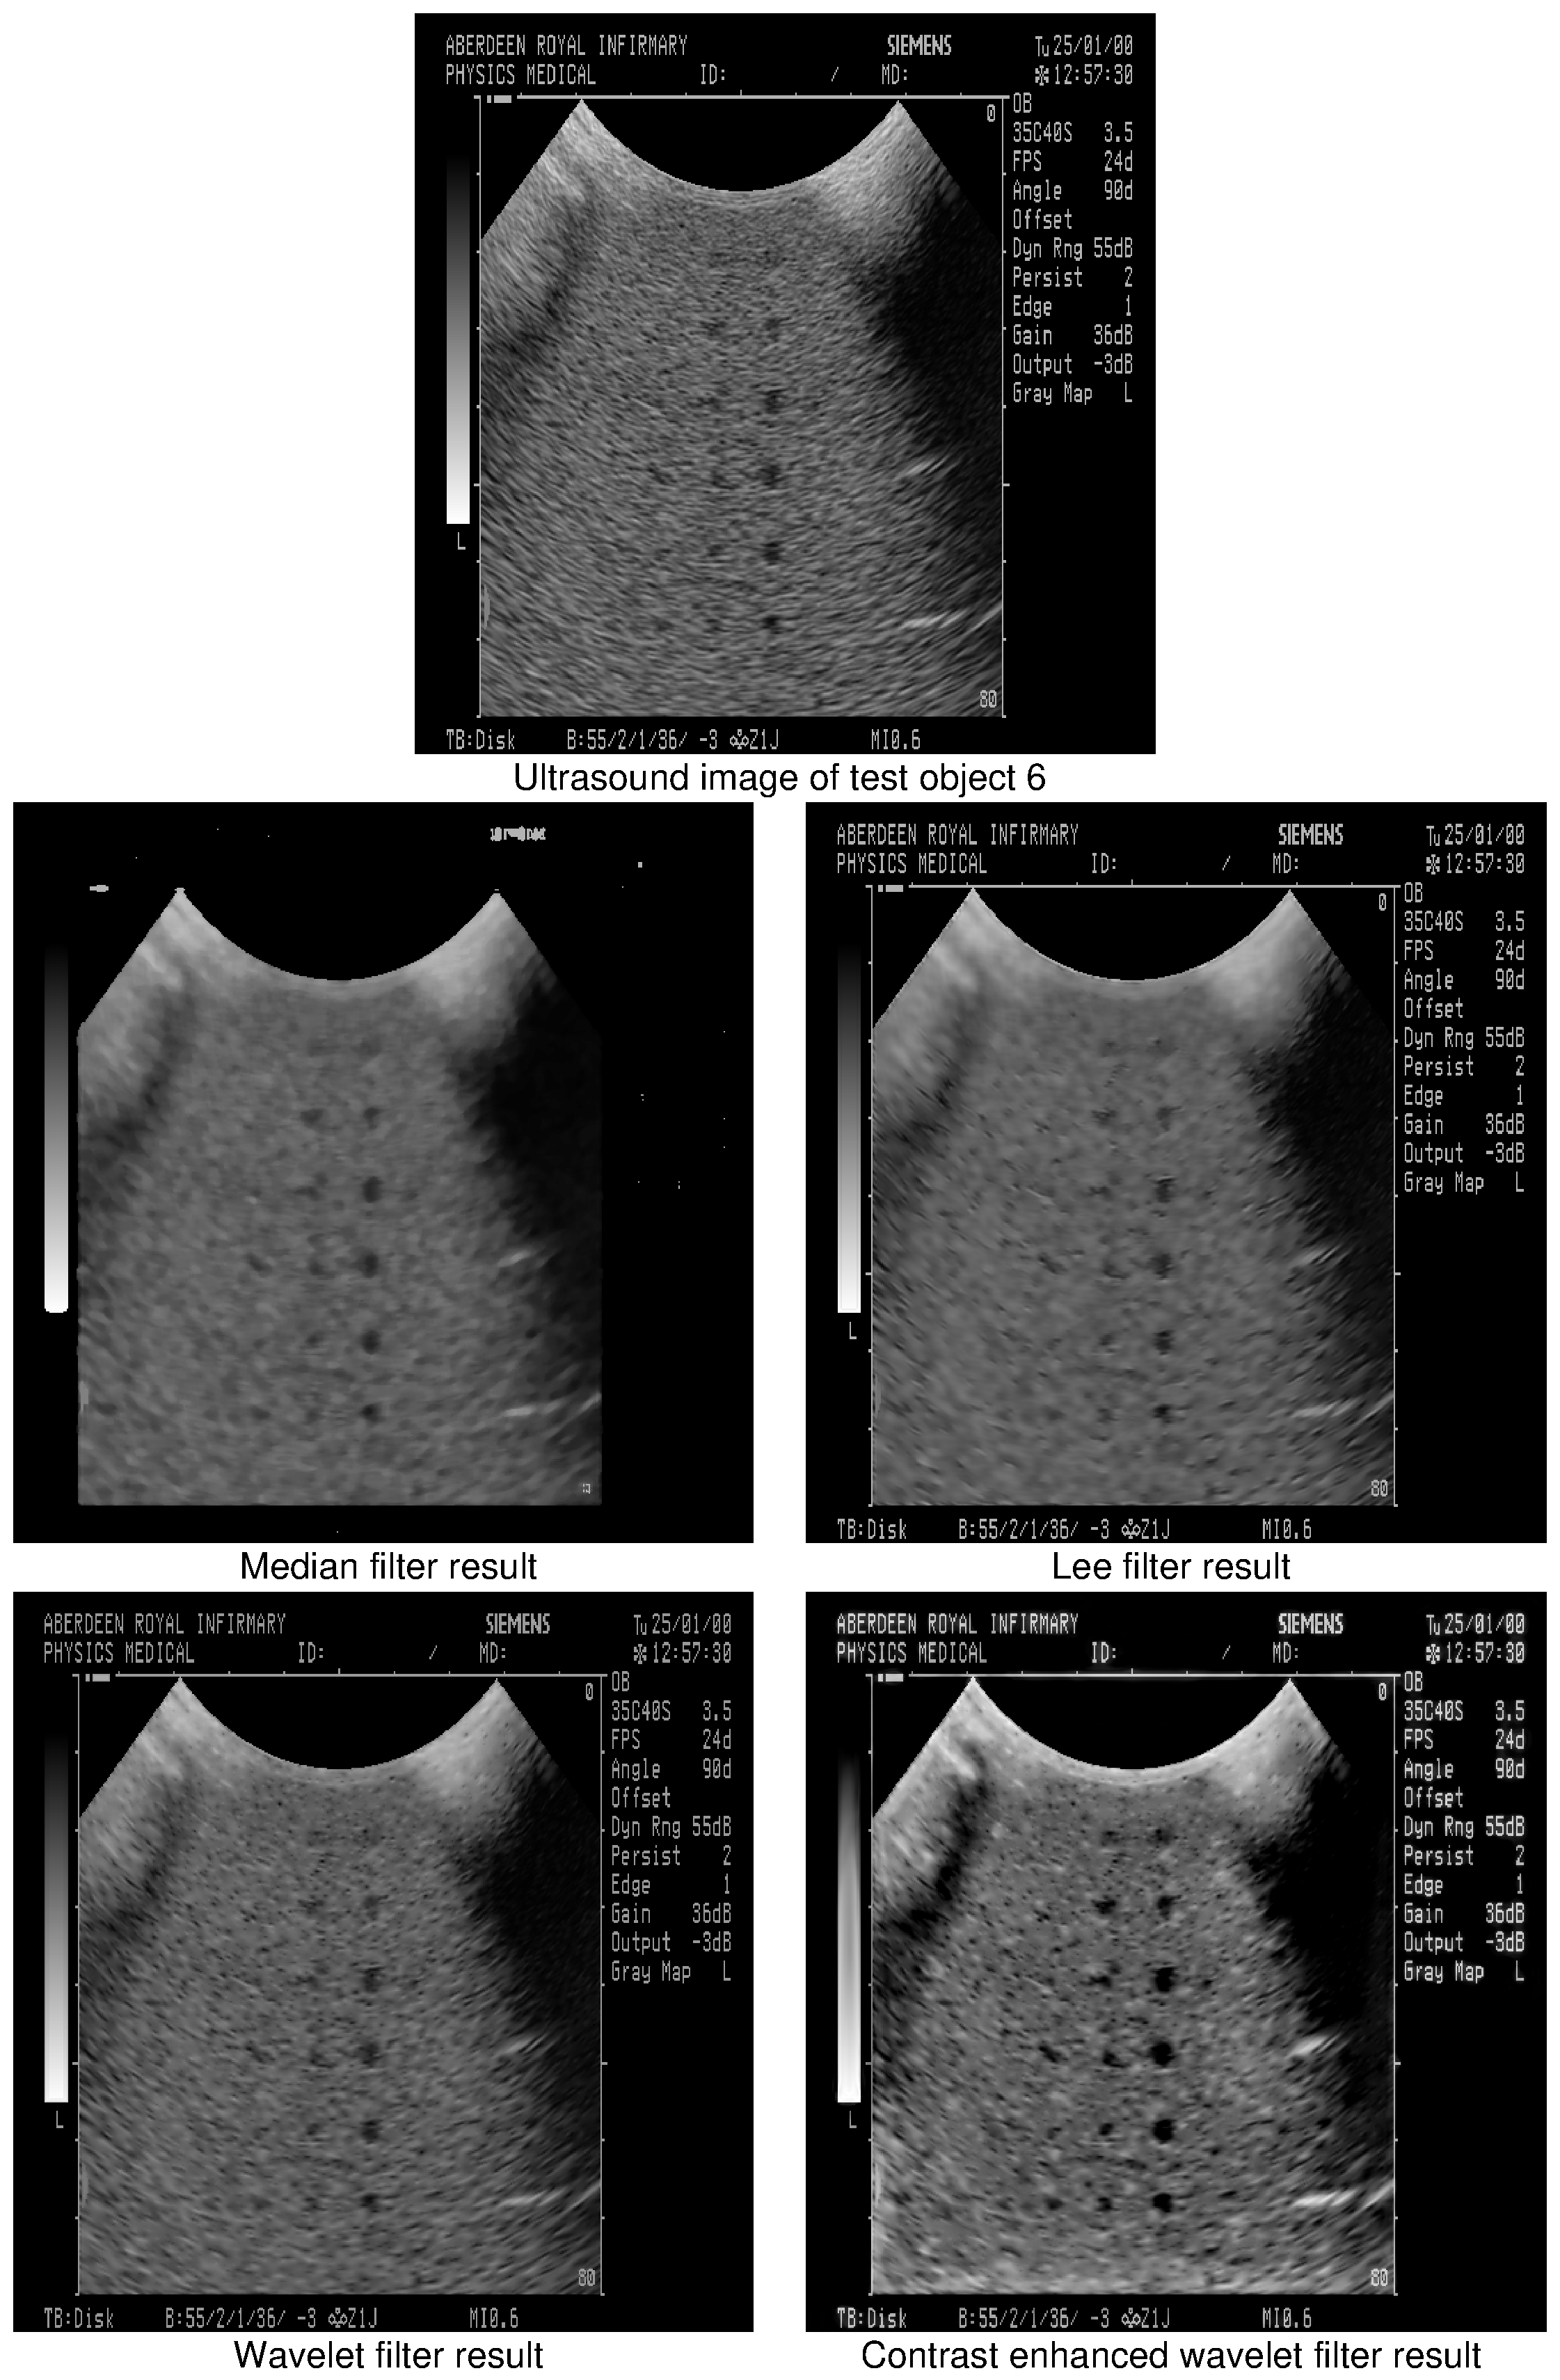
\includegraphics[width=14.5cm,height=18cm]{suitcaseResultsDenoise/wavSuit/NEW_PHYS0125.pstex}
}}
	\caption{Despeckling an ultrasound image: test object 6}
	\label{test6US}
\end{figure}


\chapter{Digital watermarking: An overview}
\label{chapter:wmIntro}
As the internet and other networked systems proliferate at ever increasing rates in today's world, the need
to provide copyright protection to digital media becomes ever more important.
Networked systems provide the benefit of allowing digital media
to be shared and distributed very easily. However, this advantage is tempered by the fact 
that a copyright violator can make perfect copies of any distributed digital media and
sell them on as pirated versions.

Logically, providers of digital media are somewhat reluctant to share and distribute their wares for 
fear of their copyright being violated.
In order to combat this problem, hiding information (\emph{e.g.}, a secret message) into the digital
media can help verify ownership of copyright.

Information hiding can be broken down into two categories: steganography and watermarking.
Steganography refers to the act of making communications invisible by using apparently
harmless messages which are in fact conveying more information than they appear to be.
As a simple example, the first letter of every paragraph in this section has been chosen to convey 
a secret message. When these letters are concatenated together, a secret message is revealed: the
name \emph{ALICE}.
The rest of the document is acting as a decoy.

Communication hiding as a method of providing copyright protection to digital media
(such as still images, audio, video and text) is called watermarking.
Unlike steganography, watermarking
implies robustness, \emph{i.e.}, watermarked digital media should be able to 
withstand non-malicious and malicious
attacks in order to preserve the copyright information that it is carrying.
Even if an attacker knows that a piece of digital media contains a watermark, it should be extremely difficult
for the attacker to remove it without knowledge of a secret key.

Enhancement and compression are examples of non-malicious attacks that a piece of watermarked digital media
may undergo. Malicious attacks refer to processes whereby someone is deliberately trying to remove a watermark
from a piece of digital media. In the case of still digital images, 
sophisticated packages such as StirMark~\cite{fab1WI, fab2WI} and unZign~\cite{unzignWIPetit}
are freely available on the internet 
which do just that.
Ideally, the copyright
information will only disappear once the watermarked digital media has been attacked to such an extent that 
it is no longer of any commercial value
(due to the quality degradation that the attack introduces to the media).

\section{General properties of watermarking systems}
All watermarking systems should adhere to the following requirements:
\begin{itemize}
	\item {\bf Imperceptibility/inaudibility}. In order to be of any use, a watermark should be as invisible/inaudible
	as possible in a piece of digital media. In order to achieve this requirement, the samples that are 
	used for watermark embedding should only be altered by small amounts. There exists a trade
	off between imperceptibility and robustness. The more robust a watermarking system is made (by increasing 
	the embedding strength) the more degraded the digital media will become.
	Thus, watermarking systems should attempt to
	maximize the energy of the embedded watermark whilst not exceeding a perceptible/audible threshold for a given
	piece of digital media.
		
	\item {\bf Redundancy}. To ensure adequate robustness, a watermark is usually embedded in a redundant
	fashion throughout a piece of digital media. This allows the watermark to be recovered from only small
	pieces of marked digital media (\emph{e.g.}, from a cropped image). Also, it compensates for the
	imperceptibility/inaudibility criterion which 
	stipulates that samples altered to carry a piece of the watermark 
	should only be altered by small amounts.

	\item {\bf Keys}. All watermarking systems should make use of secret keys. These are used to
	help randomise the process of where a watermark is to be embedded into a piece of digital media.
	If an attacker knows that a certain watermarking system has been used to mark a piece 
	of digital media, he/she will be unable to erase the watermark unless they have access to 
	the secret key as well.

\end{itemize}

\section{Types of watermarking systems}
As this thesis is concerned only with watermarking systems operating upon still digital images, the term
\emph{digital media} will be replaced with the more apt term of \emph{image}.
For an image \emph{I}, a key \emph{K} (commonly a seed to a random number generator) and a watermark \emph{W},
the embedding process common to all watermarking schemes is 
given by: $I \times K \times W \rightarrow \mbox{\emph{\~{I}}}$.
Kutter \emph{et al.} \cite{petit99} have 
identified three distinct types of watermarking systems based upon the inputs
and outputs of their extraction stage. These are:
\begin{itemize}
	\item {\bf Private watermarking} (also referred to as non-blind or non-oblivious schemes). 
	These systems must have access to the original image in the detection stage. 
	This type of watermarking scheme can be further split into two distinct types. 
	\emph{Type I} systems make use of the original image as a guide to help determine where the 
	watermark is embedded in an attacked 
	image \emph{\~{I}'} ($\mbox{\emph{\~{I}'}} \times I \times K \rightarrow W$).  
	\emph{Type II} systems require the original watermark (in addition to the original image)
	to help with the detection process. These systems report that the watermark is
	either present or not present ($\mbox{\emph{\~{I}'}} \times I \times K \times W \rightarrow \{0,1\}$).
	This type of watermarking system is expected to be more robust than the other types as
	it conveys very little information and requires access to secret material (\emph{I} and \emph{W}).
	The widely cited 
	algorithm of Cox \emph{et al.} \cite{cox1} is 
	an example of a non-blind \emph{type II} watermarking system.

	\item {\bf Semi-private watermarking} does not require the original image for watermark extraction and
	reports the presence or non-presence of a watermark
	($\mbox{\emph{\~{I}'}} \times K \times W \rightarrow \{0,1\}$).

	\item {\bf Public watermarking} (also referred to as blind or oblivious schemes).
	These neither require the original image nor the watermark in the detection process and hence
	pose the greatest challenge to the watermaking community. Only the secret key is required in the
	detection process, $\mbox{\emph{\~{I}'}} \times K \rightarrow W$. 
	Public watermarking schemes have 
	far more applications than either private or semi-private schemes in the realm of digital 
	media copyright protection. An example of this type of watermarking scheme was presented
	by Dugad \emph{et al.} \cite{dugadDI}.
	
\end{itemize}

\section{Applications for watermarks}
Depending upon the application, the requirements of watermarking systems differ based upon the
intended application area. 
\begin{itemize}
	\item {\bf Watermarking for copyright protection} deals with embedding information about 
	the copyright owner in order to prevent other parties claiming copyright ownership. This
	is the most prevalent type of watermarking system under investigation today.

	\item {\bf Fingerprinting for traitor tracking} embeds a different watermark into 
	each distributed image (not unlike a serial number). Thus, information is conveyed
	about the recipient rather than the owner and helps investigators trace back
	illegally reproduced images.

	\item {\bf Watermarking for copy protection} prevents unauthorised copying of 
	digital media. Such watermarking systems would be closed or proprietary (Digital Versatile Disc (DVD) for example)
	and would indicate the copy status of the digital media.

	\item {\bf Watermarking for image authentication} uses fragile watermarks in order to 
	detect/correct modifications in an image. Such fragile watermarking systems should have
	high robustness to compression attacks and low robustness to all other types of attack.
\end{itemize}

\section{Attacking watermarked images}
\label{sec:wmatt}
This thesis concentrates upon digital image watermarking for copyright protection.
Watermarking systems which attempt to provide copyright protection must be resilient
to different forms of attack. Such attacks include, amongst others, noise addition, compression, filtering,
cropping, resizing and rotation. 
These attacks can be grouped into two categories: (1) signal processing
attacks and (2) geometrical attacks. Signal processing attacks (\emph{e.g.} noise addition,
compression and filtering) reduce the
watermark energy within an image. After such an attack, a decoder can locate
the pixels that have been marked but it cannot necessarily detect the watermark correctly
(due to the low energy of the watermark).
Geometrical attacks (\emph{e.g.} cropping, resizing and rotation) attempt to desynchronize
the watermark at the decoder. When desynchronization occurs, the decoder cannot find the
pixels that have been marked and thus cannot detect the watermark.

This thesis focuses upon signal processing attacks only. For desychronization attacks, such
as cropping and resizing, it is assummed that the decoder has successfully
resychronized with the watermark after compensating for geometrical distortions.
A more detailed discussion of geometrical attacks and resynchronization techniques can be found in
\cite{tpunRST1, tpunRST2, tpunRST3, tpunRST4, wangRST, linRST, senRST, ozerRST, patrickBasRST, voloGreece2001, ECCb4:volo}.



\section{Contributions}
This thesis contributes in two different areas to the field of digital image watermarking.
Firstly, a novel and robust watermarking system is presented in Chapter \ref{chapter:dugInoue} which aims
to provide copyright protection to digital images.
This is a blind and quantization based watermarking scheme operating within the wavelet domain. 
Results show that this novel watermarking scheme produces watermarked images with very little degradation which are robust 
to many forms of attack.

Secondly, fair comparisons of the effects of ECCs on different digital image watermarking
algorithms are made in Chapters 
\ref{chapter:80_320} and
\ref{chapter:BK}.
The motivation for these fair comparisons arose from the fact that many authors use ECCs, such as
repetition and BCH codes, in their watermarking systems (see Chapter \ref{chapter:eccB4}). 
However, many of these authors do not make a comparison 
between uncoded watermarks and watermarks which incorporate ECCs. 
It is shown in the results that it is not always beneficial to include ECCs in a watermarking system.


\chapter{A novel, blind and robust watermarking scheme}
\label{chapter:dugInoue}
In the following sections, a quantization based watermarking method operating within
the wavelet domain will be presented.
This new scheme utilises implicit visual masking by only inserting a watermark bit into 
coarse wavelet coefficients of high magnitude. 
Also, this watermarking technique is blind (\emph{i.e.}, neither the original uncorrupted image
nor any side information is required in the recovery process) as well as being very 
computationally efficient.
This new watermarking algorithm combines and adapts various aspects from two existing watermarking methods
\cite{dugadDI, inoueDI}. Results show that the newly presented method improves upon both
of these existing techniques.

\section{Review of Dugad's watermarking scheme}
Previously, Dugad \emph{et al.}~\cite{dugadDI} presented an additive watermarking method operating 
in the wavelet domain. The most novel aspect of this scheme was the introduction of
an \emph{image sized watermark}. 
This allowed the scheme to detect a watermark without access to the original uncorrupted
image (as opposed to the scheme described by Cox \emph{et al.}~\cite{cox1}).

But why is it advantageous to have access to the original uncorrupted image in the detection process
(\emph{i.e.}, non-blind watermarking)? 
Robustness dictates that a watermark should be added to the perceptually significant 
coefficients of an image; this makes it difficult to remove the watermark without
causing a great deal of degradation to the watermarked image.
However, in the recovery process, the order and amount 
of these perceptually significant coefficients may be altered due to various image 
manipulations. Hence, the original image is useful in determining the locations of where
the watermark has been inserted.
The drawback of non-blind watermarking schemes is that they require access
to the secret uncorrupted original image. It is therefore desirable to create 
watermarking systems which are both robust and blind. 

In \cite{pivaDI}, Piva \emph{et al.} presented a blind watermarking scheme. This scheme required 
the watermark to be inserted into 25000 DCT coefficients (which are not necessarily perceptually 
significant) as opposed to only 1000 in the
non-blind Cox method. Since such a large watermark is added using this method, visual masking 
is performed in the spatial domain prior to insertion in order to prevent the 
watermarked image from becoming too degraded. As this visual masking cannot be taken into 
account in the detection process as well as the non-presence of the original uncorrupted image,
the detector response for this scheme is comparatively poor.

Dugad's watermarking scheme improves upon the Piva method, as implicit visual masking 
is employed (as opposed to Piva's explicit visual masking). This ensures that only the
perceptually significant coefficients are selected for watermark insertion. Dugad's scheme is also 
image specific in that it adapts the watermark length depending upon the smoothness of
the image. For example, less watermark bits are added to smooth images and more watermark bits are added to
busy images.

In the insertion stage of Dugad's algorithm, all wavelet coefficients\footnote{a three level Discrete Wavelet Transform (DWT) with 
a Daubechies 8-tap filter was used} (barring the lowpass component)
of magnitude greater than \emph{T1} are selected.
This ensures that only perceptually significant 
coefficients are used (implicit visual masking). The amount of wavelet coefficients of 
magnitude greater than \emph{T1} will depend upon the smoothness/busyness of the image. 
A watermark (of zero mean and unit variance) equal in size to the input 
image is generated with a known seed value. 
At a location where a wavelet coefficient magnitude is
greater than \emph{T1}, the watermark value at the same location in the image sized watermark
is added to it via:
\begin{equation}
	\hat{w}_{ij} = w_{ij} + \alpha |w_{ij}| x_{ij}
\end{equation}
where $w_{ij}$ is the wavelet coefficient, $\alpha$ is a scaling parameter, $ x_{ij}$
is a watermark value and $ \hat{w}_{ij}$ is the watermarked wavelet coefficient.

In the recovery process, the image sized watermark is regenerated using the known seed value.
Then all wavelet coefficients (barring the lowpass component)
of magnitude greater than \emph{T2} from a possibly corrupt watermarked image are selected. 
Note that by setting \emph{T2} $>$ \emph{T1} the
robustness of the algorithm is increased, as the magnitude of some wavelet coefficients, 
which were originally below \emph{T1},
may become greater than \emph{T1} due to image manipulations.
Only wavelet coefficients with  magnitude greater than \emph{T2} are 
used in the detection process; these are correlated with the 
watermark values (from the regenerated image sized watermark) at the same locations.
After this correlation process, a yes or no answer will be given 
as to the presence of the watermark. Both the insertion (top half) and detection (bottom half) processes are
shown in Figure \ref{dugFlowDI}.

\begin{figure}[htb]
\setlength{\abovecaptionskip}{-0.2cm}
	\begin{center}
		\includegraphics[width=13cm]{dugFlow.pstex}
	\end{center}
	\caption{Overview of Dugad's watermarking scheme} 
	\label{dugFlowDI}
\end{figure}
 
\section{Review of Inoue's watermarking scheme}
Two watermaking algorithms were presented by Inoue \emph{et al.}~in~\cite{inoueDI}.
Both algorithms were implemented in the wavelet domain but each targeted a different
set of coefficients for insertion. The first of these insertion techniques
operated upon insignificant coefficients\footnote{the insignificant coefficients were chosen based 
upon the calculation of zerotrees}
whereas the second insertion technique operated 
upon significant coefficients. 
Thus, both insertion techniques could be applied to a single
image at the same time. However, the reported results indicate that the insertion technique utilising the
significant coefficients was more robust than the insertion technique operating
upon the insignificant coefficients. For this reason, only the insertion
technique utilising the significant coefficients will be considered. 

This method takes a three level wavelet transform\footnote{implemented via 5/3 taps
symmetric short kernel filters} of the image to be watermarked and
inserts the watermark into the 
detail coefficients at the coarsest scale, \emph{i.e.}, wavelet level three.
The detail coefficients at level three are the horizontal details, High Low 3 (HL3),
the vertical details, Low High 3 (LH3) and the diagonal details, High High 3 (HH3). 
The lowpass component, Low Low 3 (LL3), is left unchanged.
This is a quantization\footnote{where a message is embedded by mapping selected pixels to predefined intervals} based watermarking technique 
which aims to modify 
wavelet coefficients of high magnitude thus embedding the watermark into 
edge and textured regions of an image. The process for watermark insertion is as follows:
\begin{enumerate}
	
	\item Two thresholds, \emph{T1} and \emph{T2}, are selected and any one
	of the subbands LH3, HL3 or HH3 is chosen. Next, 
	significant coefficients $C_{k} (k=1,2,\cdot\cdot\cdot, N)$ satisfying 
	$\mbox{\emph{T1}} < |C_{k}| < \mbox{\emph{T2}}$ are found. 
	
	\item A binary watermark is created, $W(k), k=1,2,\cdot\cdot\cdot, N$. 
	
	\item For $k = 1, 2, \cdot\cdot\cdot, N$, the watermark is embedded by 
	modifying $|C_{k}|$ as follows: \\
	If $W(k) = 1$ and $C_{k} > 0$, then $C_{k} = \mbox{\emph{T2}}$, \\
	If $W(k) = 0$ and $C_{k} > 0$, then $C_{k} = \mbox{\emph{T1}}$, \\
	If $W(k) = 1$ and $C_{k} < 0$, then $C_{k} = \mbox{\emph{-T2}}$ \\
	If $W(k) = 0$ and $C_{k} < 0$, then $C_{k} = \mbox{\emph{-T1}}$

	\item Save the embedded position, subband label and the 
	thresholds \emph{T1} and \emph{T2}.
\end{enumerate}

The following process details the steps involved for watermark detection:
\begin{enumerate}
	\item Using the subband label and the embedded position, the
	recovered wavelet coefficients $C_{k}^{'}, k = 1,2,\cdot\cdot\cdot, N$ are obtained.

	\item Check each $C_{k}^{'}$ individually: \\
	If $|C_{k}^{'}| < (\mbox{\emph{T1}} + \mbox{\emph{T2}}) / 2$, then the
	recovered watermark bit is a 0. \\
	If $|C_{k}^{'}| \geq (\mbox{\emph{T1}} + \mbox{\emph{T2}}) / 2$, then the
	recovered watermark bit is a 1. 
\end{enumerate}

\section{Dugad and Inoue: Advantages and disadvantages}
Advantages of the Dugad algorithm:
\begin{itemize}
	\item It is a blind algorithm. Only the seed value for regenerating the 
	image sized watermark and
	the threshold value \emph{T2} are needed to detect the watermark.
	\item It uses implicit visual masking. Thus, the watermark is inserted
	into the perceptually significant areas of an image via a simple
	and straightforward process.
\end{itemize}
Disadvantages of the Dugad algorithm:
\begin{itemize}
	\item It embeds the watermark in an additive fashion.
	This is a drawback as blind detectors for additive watermarking schemes must correlate the
	possibly watermarked image coefficients with the known
	watermark in order to determine if the image has or has not 
	been marked. Thus the image itself must be treated as noise 
	which makes detection of the watermark exceedingly difficult \cite{meerMasters}.
	In order to overcome this, it is necessary to correlate a very high number
	of coefficients (which in turn requires the watermark to be embedded into many
	image coefficients at the insertion stage). This has the effect of decreasing
	the robustness of the watermarking scheme as well as causing greater degradation
	to the marked image.
	\item The detector can only tell if the watermark is
	present or absent. It cannot recover the actual watermark.
\end{itemize}
Advantages of the Inoue algorithm:
\begin{itemize}
	\item It uses a scalar quantization process to embed the 
	watermark. This is an advantage as quantization
	based watermarking schemes, unlike additive watermarking schemes, do not suffer from host image
	interference \cite{meerMasters}.	
	Hence, detectors from quantization
        based watermarking techniques can operate successfully using a much smaller
	watermark than is possible for additive schemes. This has the knock-on effect
	of increasing robustness as well as reducing the amount of degradation suffered 
	by a marked image.
	\item The detector can recover the binary watermark
	sequence thereby allowing the user to see it.
	\item It inserts the watermark into perceptually significant wavelet coefficients.
\end{itemize}
Disadvantages of the Inoue algorithm:
\begin{itemize}
        \item It is a semi-blind algorithm as it
	requires a file containing the locations of where the watermark
	was embedded in order for the detector to work. 
\end{itemize}

\section{A novel approach}
The Dugad and Inoue schemes are quite similar in that they both use two threshold values and
they both operate in the wavelet domain. 
Nevertheless, as previously pointed out, both have
advantages and disadvantages. However, combining both schemes in a judicious fashion can result in 
a new method which shares the advantages of both schemes whilst discarding most of the disadvantages.
This can be achieved by using Dugad's idea of an image sized watermark in conjunction with
adapted versions of Inoue's scalar quantization insertion/detection techniques.
The resulting algorithm then has the following features:
\begin{itemize}
 	\item It is completely blind (unlike the semi-blind scheme of Inoue).
	\item It is a quantization based technique (unlike the Dugad method).
	This allows:
	\begin{itemize}
		\item The user to view a recovered watermark.
		\item Less coefficients to be marked thereby producing watermarked images 
		with very little degradation.  
		This is possible as detectors for quantization 
		based schemes do not suffer from host image noise (unlike additive schemes).
		Thus, they do not require a large amount of coefficients to be marked 
		to achieve reliable detection.
	\end{itemize}
	\item It employs implicit visual masking as only wavelet coefficients
	of high magnitude at the third level are considered for watermark embedding.
	These are perceptually significant coefficients thus making the scheme robust.
	Also, these coefficients correspond to edge and texture regions of images and are
	thus best suited for creating watermarked images that do not appear degraded 
	to human viewers.
	\item 
	It uses a watermark the same size as the third level subband images (as opposed
	to Dugad's method of an image sized watermark). This is done as only the third
	level wavelet coefficients are to be marked (hence creating an image sized watermark
	would be redundant). 
	This third level subband sized watermark negates the need for 
	a position file in the recovery process (thereby improving upon the Inoue scheme). 
\end{itemize}
In summary, this new technique improves upon the Dugad method by using a 
quantize and replace insertion process (rather than an additive insertion process).
Thus, for comparable robustness performance, the new method will produce watermaked images
with less degradation than the Dugad scheme.
It improves upon the Inoue scheme
by having no need for a position file in the recovery process.





\section{Implementation of the novel approach}
A flow diagram detailing the necessary steps is shown in Figure \ref{novelAlgDI},
where the top part shows the insertion process and the bottom part shows the detection process.
The quantization and dequantization steps are explained in more
detail in Sections \ref{sub:embedDI} and \ref{subsec:detDI}, respectively.
\begin{figure}[htb]
\setlength{\abovecaptionskip}{-0.2cm}
	\begin{center}
		\includegraphics[height=7.5cm,width=13cm]{novelAlg3.pstex}
	\end{center}
	\caption{Overview of the novel, blind and quantized based watermarking scheme} 
	\label{novelAlgDI}
\end{figure}

\subsection{Embedding}
\label{sub:embedDI}
The watermark embedding process transforms the host image into the wavelet domain\footnote{the
current implementation uses Daubechies wavelets of length 4}. Next, all the coefficients in the third
wavelet level (excluding the \emph{low/low} subband) with magnitude
greater than \emph{T1} and magnitude less than \emph{T2} are selected. 
A binary watermark
the same size as the 
entire third level of the wavelet transform
is created using a secret key (which is a seed to a random
number generator). The selected wavelet coefficients are then quantized 
in order to embed a watermark bit. 
The value that the selected coefficients are quantized to depends upon
whether they are embedding a 1 or a 0. A selected wavelet coefficient, $w^{s}_{ij}$,
will embed a 1 if the value in the watermark file at the same location, $x_{ij}$, is 1.
Alternatively, $w^{s}_{ij}$ will embed a 0 if $x_{ij}$ is 0.
The quantization method is similar to that used by Inoue: \\
If $x_{ij} = 1$ and $w^{s}_{ij} > 0$, then $w^{s}_{ij} = \mbox{\emph{T2 - X1}}$, \\
If $x_{ij} = 0$ and $w^{s}_{ij} > 0$, then $w^{s}_{ij} = \mbox{\emph{T1 + X1}}$, \\
If $x_{ij} = 1$ and $w^{s}_{ij} < 0$, then $w^{s}_{ij} = \mbox{\emph{-T2 + X1}}$ \\
If $x_{ij} = 0$ and $w^{s}_{ij} < 0$, then $w^{s}_{ij} = \mbox{\emph{-T1 - X1}}$ \\
The \emph{X1} parameter narrows the range between the two quantization values of \emph{T1}
and \emph{T2} in order
to aid robust oblivious detection (see Section \ref{subsec:detDI}).

After all the selected coefficients have been quantized, the inverse wavelet 
transform is applied to all the wavelet coefficients and the watermarked image
is obtained.

\subsection{Detection}
\label{subsec:detDI}
For oblivious detection, the wavelet transform of a possibly corrupted
watermark image is taken. Then all the wavelet coefficients of magnitude greater than
or equal to \emph{T1 + X2} and less than or equal to \emph{T2 - X2} are selected;
these shall be denoted via $w'^{s}_{ij}$.

Note that \emph{X2} should be less than \emph{X1}. Figure \ref{newQuantDI} shows the need to introduce
the new parameters of \emph{X1} and \emph{X2} (this figure shows the quantization process for 
\emph{positive} valued wavelet coefficients).
In the insertion process, all wavelet coefficients
with a magnitude greater than \emph{T1} and less than \emph{T2} are selected and then quantized to
either \emph{T1 + X1} or \emph{T2 - X1}. In the recovery process, all the wavelet coefficients
of magnitude greater than or equal to \emph{T1 + X2} and less than or equal to \emph{T2 - X2} are 
selected to be dequantized.
This helps ensure that all the marked coefficients are recovered and dequantized after
being attacked. Also, 
unmarked coefficients are unlikely to drift into the range of selected coefficients
after an attack. The introduction of the \emph{X1} and \emph{X2} parameters to the watermarking algorithm
gives a degree of tolerance to the system against attacks, \emph{i.e.}, they collaborate to give a \emph{noise margin}.

\begin{figure}[htb]
\setlength{\abovecaptionskip}{-0.2cm}
	\begin{center}
		\includegraphics[height=8.5cm,width=13cm]{newQuant3.pstex}
	\end{center}
	\caption{Insertion and detection methods for the novel watermarking scheme}
	\label{newQuantDI}
\end{figure}

A watermark
bit is decoded for each of the selected wavelet coefficients via the same process
described by Inoue: \\
If $|w'^{s}_{ij}| < (\mbox{\emph{T1}} + \mbox{\emph{T2}}) / 2$, then the
recovered watermark bit is a 0. \\
If $|w'^{s}_{ij}| \geq (\mbox{\emph{T1}} + \mbox{\emph{T2}}) / 2$, then the
recovered watermark bit is a 1. 

The recovered watermark is then correlated with the original copy of the
watermark file (obtained via the secret key) only in the 
locations of the selected coefficients. This allows a confidence measure
to be ascertained for the presence or non-presence of a watermark in an 
image.

\section{Results}
This section outlines the results obtained by Dugad's scheme and the newly 
proposed scheme. It is the aim of the new scheme to be as robust as
the Dugad scheme without degrading the marked images to the same extent. 
Because this new scheme has the advantageous property of not requiring a
position file in the recovery process, it cannot match the robustness
performance presented by Inoue. However, this is to be expected as 
non-blind and semi-blind watermarking schemes gain robustness via
the secret information (\emph{e.g.}, uncorrupted original images and position files)
that the detectors require.

\subsection{Dugad's results}
In Dugad's paper, the response of the detector to various attacks was presented.
However, a measure of the image degradation was not reported (only a watermarked
image was presented for visual inspection). Thus, in order to ascertain a measure
of the image degradation suffered due to Dugad's scheme, it is necessary to 
encode the scheme to reproduce the same results and then obtain a quantitative
measure of the image degradation. In order to achieve this, the same image 
that Dugad used will be used here; \emph{i.e.}, Lena (8-bit greyscale, $256 \times 256$). Both
the PSNR and the TPE (Section~\ref{perceptualMetrics}) between the original and
the watermarked images are computed. 
The Checkmark package \cite{ChkMrk:pereiraDI} (\emph{WatsonMetric.m}) was used to determine the TPE.

Another consideration 
to note about the results presented by Dugad is that
only a single seed value (of 100) was used 
for each attack.
This is important as the
random number generator used by Dugad will almost certainly 
be different from 
the one used here. In order to accommodate this, the same attack was performed
thirty times upon the Lena image which had a watermark inserted using a different seed value each time. The 
average of the results was then taken and are shown in Table \ref{dugResultsDI}.
Figures \ref{originalLenaDI} and \ref{lenaDugDI} show the original Lena image and a Lena image watermarked
via Dugad's scheme (seed value = 100, $\alpha$ = 0.2, \emph{T1} = 40 and \emph{T2} = 50), respectively.
\begin{figure}[p]
\setlength{\abovecaptionskip}{0.1cm}
	\begin{center}
		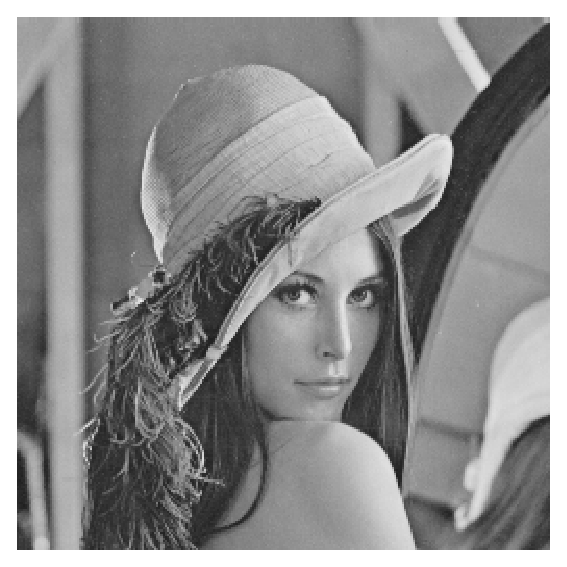
\includegraphics[height=8cm,width=8cm]{IM_originalLena.ps}
		\caption{Original Lena image}
		\label{originalLenaDI}
	\end{center}
\end{figure}
\begin{figure}[p]
\setlength{\abovecaptionskip}{0.1cm}
	\begin{center}
		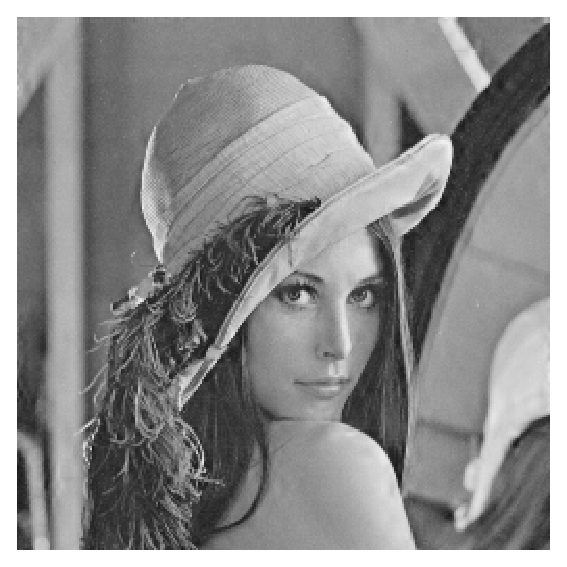
\includegraphics[height=8cm,width=8cm]{IM_dugSeed100Lena.ps}
		\caption{Lena watermarked with Dugad's scheme}
		\label{lenaDugDI}
	\end{center}
\end{figure}


\subsection{Discussion of Dugad's results}
The results obtained here are very similar to the results reported by Dugad.
Note that more attacks are studied here than were studied in the Dugad paper
(which consisted of: no attack, JPEG Quality Factor (QF) 5 attack, 
``cropping'' attack, median filtering
attack (with a $5 \times 5$ window), Gaussian 
noise attack ($\sigma^2=600$\footnote{approximately equivalent to a normalised variance of 0.0092})
and a ``half sizing'' attack (where the image was half sized and then resampled back to its original size)).
\begin{table}[!t]
\begin{tiny}
\centerline{
\begin{tabular}{|p{1.7cm}|c|c|c|c|c|c|c|c|c|c|} \hline
& No &\multicolumn{3}{|c|}{JPEG} & \multicolumn{2}{|c|}{Median filter} 
	& Gaussian & Impulse & ``Cropp- & ``Half \\ \cline{3-7}   
& attack &  QF 5& QF 10 & QF 15 & $3 \times 3$ & $5 \times 5$ 
	& $\sigma^{2}=375$ & Noise & ing'' & sizing'' \\ \hline
\underline{Correlation} & & & & & & & & & & \\
- Average & 32.43 & 12.17 & 17.83 & 20.85 & 25.16 & 17.74 & 14.57 & 12.96 & 22.04 & 16.16 \\ 
- Std. & 2.46 	& 2.78    & 2.56  & 2.68  & 3.68  & 2.80  & 1.42  & 1.58  & 3.49  & 2.32 \\ 
- Minimum & 27.44 	& 7.01    & 11.95 & 14.86 & 17.56 & 11.21 & 12.43 & 9.55  & 14.26 & 12.22 \\
- Maximum & 38.35 	& 18.35   & 23.36 & 24.43 & 32.66 & 21.45 & 18.83 & 16.21 & 29.07 & 21.03 \\\hline
Average detector threshold & 9.00 & 9.12 & 9.20 & 9.16 & 9.26 & 9.38 & 7.77 & 8.04 & 9.83 & 8.51 \\ \hline 
Average length of WM in & 2552 & 2552 & 2552 & 2552 & 2552 & 2552 & 2552 & 2552 & 2552 & 2552 \\ \hline 
Average length of WM out & 1788 & 1534 & 1560 & 1617 & 1274 & 933 & 3151 & 3920 & 1016 & 1957 \\ \hline 
Average PSNR (dB) & 37.38 & 37.40 & 37.50 & 37.42 & 37.29 & 37.52 & 37.24 & 37.43 & 37.39 & 37.27 \\ \hline 
Average TPE & 0.014 & 0.014& 0.014& 0.014& 0.014& 0.014& 0.014& 0.014& 0.014& 0.014\\ \hline 
Failures & 0 & 5 & 1 & 0 & 0 & 0 & 0 & 0 & 0 & 0 \\ \hline 
\end{tabular}}
\end{tiny}
\renewcommand{\baselinestretch}{1.5}
\caption{Dugad system robustness, using Lena image, to various attacks }
\label{dugResultsDI}
\end{table}
The attacks performed here and presented in Table~\ref{dugResultsDI} are: 
JPEG compression to quality 5, quality 10 and quality 15; median filtering 
with windows of $3\times3$ and $5\times5$; Gaussian noise addition 
($\sigma^{2}=375$\footnote{approximately equivalent to a normalised variance of 0.0058}); 
impulse noise addition
(normalised variance of 0.015); ``cropping'' the image from rows 60 to 190 and from columns 60 to 190
(these crop values were estimated by visually studying the cropped image in the Dugad paper);
``half sizing'' 
(where the image is subsampled by two and then resized back to its original size).
Using these attack parameters, the correlation values reported in the Dugad paper have been 
reproduced here. 
In Table~\ref{dugResultsDI}, the correlation and detector threshold were calculated via:
\begin{equation}
	correlation=\frac{1}{N} \sum^{N}_{i} \hat{w}_{i}x_{i}
\end{equation}
\begin{equation}
detector~threshold = \frac{\alpha}{2N} \sum^{N}_{i} |\hat{w}_{i}|
\end{equation}
where $\hat{w}_{i}$ is a watermarked image coefficient in the wavelet domain, $x_{i}$ is a watermark 
coefficient, $N$ is the number of coefficients used by the decoder and $\alpha$ is a weighting factor.

Note that the ``crop'' attack performed by Dugad does not desychronize the decoder
like a true geometrical attack should (see Section~\ref{sec:wmatt}).
Rather, the ``crop'' attack performed by Dugad creates 
a border of zeros in the image. This has the effect of reducing the watermark energy. Similarly,
the ``half sizing'' attack performed by Dugad is not a geometrical attack as the image is resampled back to its
original size afterwards. Like the ``crop'' attack, 
the ``half sizing'' attack only reduces the watermark energy within
the image, it does not introduce any synchroniztion problems at the decoder. 

It was reported in~\cite{dugadDI} that the Dugad scheme
could successfully resist (returning a correlation value of 15.00) 
a Gaussian noise ($\sigma^{2}=600$) attack. However, this result could not
be reproduced here by averaging the correlations over thirty trials (see Table~\ref{tab:gaus600dug},
which details
the results for attacking a Dugad watermarked 
($\alpha$ = 0.2, \emph{T1} = 40 and \emph{T2} = 50) Lena image thirty times (different seed 
each time) with Gaussian noise ($\sigma^{2}=600$)).
\begin{table}[ht]
\setlength{\abovecaptionskip}{-0.2cm}
\begin{center}
\begin{tiny}
\begin{tabular}{|l|l|} \hline
			& Gaussian noise \\ 
			& $\sigma^{2}=600$ \\ \hline
\underline{Correlation} & \\ 
- Average	& 11.35 \\ 
- Std. 		& 1.31	\\ 
- Minimum	& 8.30	\\ 
- Maximum	& 14.76	\\ \hline
Average detector threshold & 7.86 \\ \hline
Average length of WM in	& 2552 \\ \hline
Average length of WM out& 4036 \\ \hline
Average PSNR (dB) & 37.15	\\ \hline
Average TPE & 0.014	\\ \hline
Failures 	& 0 \\ \hline
\end{tabular}
\end{tiny}
\end{center}
\caption{Dugad system robustness, using Lena image, to Gaussian noise ($\sigma^{2}=600$) attacks}
\label{tab:gaus600dug}
\setlength{\abovecaptionskip}{0cm}
\end{table}
From Table~\ref{tab:gaus600dug}, it can be seen that the Gaussian noise attacks of variance 600 are being
reliably withstood. The correlation value of 15.00 reported by Dugad for Gaussian noise ($\sigma^{2}=600$) attacks
can be attributed to only running the test once and obtaining a larger than average correlation value.

It is worth noting that the Dugad algorithm is perhaps not as robust as
was first reported. For example, in the JPEG quality 5 attack tests,
the watermark failed to be detected in five out of the thirty attacks.
In the case
of the JPEG quality 10 attacks, the watermark failed to be detected once
out of the thirty trials. Only for the JPEG quality 15 attacks was the watermark
detected every time. 

The fact that the Dugad scheme does not appear to be as robust to JPEG compression
as was first reported may be attributed to which software package was used to implement the
JPEG compression; Dugad does not mention which software package was used to perform
JPEG compression. This is important as the JPEG quality ratings between different software packages are not standardized.
For all the tests performed in this thesis, MATLAB 6.0.0.88, Release 12, was used. JPEG compression
was carried out via the \emph{imwrite} function which uses the Independent JPEG Group's (www.ijg.org) LIBJPEG library.

Further confirmation of the quantitative image quality values was obtained by 
using a secondary implementation of the Dugad algorithm available from 
\cite{meerMasters}. For thirty trials, each with a different seed value,
the average PSNR was 37.94 dB and the average TPE was 0.013 
(using a block size of $8 \times 8$).
This helps to validate the results in Table
\ref{dugResultsDI}, where the average PSNR is 37.38 dB and the
average TPE is 0.014 (again using blocks of size $8 \times 8$).

\subsection{Novel approach results}
\label{ourResultsLenaDI}
The same attacks used to test the Dugad algorithm (presented in Table
\ref{dugResultsDI}) were used to test the new algorithm (presented in Table
\ref{ourResultsDI}). \emph{T1} = 115, \emph{T2} = 200, \emph{X1} = 20 and \emph{X2} = 10
were the parametric values used; Figure \ref{lenaNewPrettyDI} shows an example
of the Lena image marked using these values and Figure \ref{allAttacksDI} shows
the results of attacking this watermarked image with:
(a) JPEG quality 5, (b) JPEG quality 10, (c) JPEG quality 15,
(d) median $3 \times 3$, (e) median $5 \times 5$, (f) Gaussian noise ($\sigma^{2}=375$),
(g) impulse noise (normalised density of 0.015), (h) ``cropping'' 
(from rows 60 to 190 and from columns 60 to 190) and (i) ``half sizing''
(followed by resizing back to the original size).
\begin{figure}[htb]
	\begin{center}
		\includegraphics[height=8cm,width=8cm]{IM_seed100_115_200_20_10.ps}
		\caption{Lena watermarked with the novel scheme}
		\label{lenaNewPrettyDI}
	\end{center}
\end{figure}
\begin{figure}[p]
\setlength{\abovecaptionskip}{-0.2cm}
	\centerline{ \hbox{
		\includegraphics[height=16cm,width=15cm]{attackPics.pstex}
	}}
		\caption{Attacking the watermarked Lena image; (a) JPEG quality 5, (b) JPEG quality 10, 
		(c) JPEG quality 15,
		(d) median $3\times3$, (e) median $5\times5$, (f) Gaussian noise ($\sigma^{2}=375$), 
		(g) impulse noise (normalised density of 0.015)
		(h) ``cropping'' (from rows 90 to 160 and columns 60 to 190), 
		(i) ``half sizing''
		(image subsampled by two then resized back to original size)}
		\label{allAttacksDI}
\end{figure}

The Normalised Correlation (NC) between two binary vectors (\emph{i.e.} the original and recovered watermarks)
can be calculated from equation~\ref{eq:nc} (and its accompanying pseudo-code in Section~\ref{sec:withPfp}). 
An analysis of the probability of obtaining a false positive ($P_{fp}$)
detector response is studied in 
Table \ref{PfpResDI} (for \emph{T1} = 115, \emph{T2} = 200, \emph{X1} = 20 and \emph{X2} = 10). 
In this study, the
lowest recorded NC value
and the lowest recorded recovered watermark length
from the thirty trials (using a different seed each time) were saved.
Using these values, it is possible to calculate the probability of obtaining a false 
positive reading \cite{kundurPfpDI}. This is a \emph{worst case} scenario of obtaining a false positive
detection as the lowest NC and the smallest recovered watermark length are being used in the calculation
(even though these two values did not occur simultaneously in any of the trials for any of the attacks).
The probability of obtaining a false positive reading is calculated via: 
\begin{equation}
\label{eq:PfpBKX_di}
        P_{fp} = \sum^{N_{w}}_{n= \lceil N_{w}(T+1)/2 \rceil} \left(
                                                                        \begin{array}{c}
                                                                                N_{w} \\
                                                                                n
                                                                        \end{array}
                                                              \right)                           0.5^{N_{w}}
\end{equation}
where $N_{w}$ is the length of the recovered watermark and $T$ is the chosen detector threshold value.
More information regarding the calculation of $P_{fp}$ values is given in Section~\ref{sec:withPfp}.

\begin{table}
\begin{tiny}
\centerline{
\begin{tabular}{|p{1.85cm}|c|c|c|c|c|c|c|c|c|c|} \hline
& No &\multicolumn{3}{|c|}{JPEG} & \multicolumn{2}{|c|}{Median filter} 
	& Gaussian & Impulse & ``Cropp- & ``Half \\ \cline{3-7}  
& attack & QF 5 & QF 10 & QF 15 & $3 \times 3$ & $5 \times 5$ 
	& $\sigma^{2}=375$ & Noise & ing'' & sizing'' \\ \hline   
\underline{NC values} &&&&&&&&&&\\
- Average & 1.00 & 0.20 & 0.62& 0.84 & 0.89& 0.30& 0.52& 0.68& 0.53& 0.51\\ 
- Std.  &0.00&0.07&0.06&0.03&0.03&0.06&0.06&0.05&0.09&0.06\\
- Minimum &1.00&0.03&0.56&0.78&0.82&0.23&0.45&0.62&0.43&0.42\\
- Maximum &1.00&0.27&0.77&0.92&0.93&0.45&0.74&0.85&0.80&0.62\\\hline
Detector threshold chosen & 0.40 & 0.40 & 0.40 & 0.40 & 0.40 & 0.40 & 0.40 & 0.40 & 0.40 & 0.40   \\ \hline
Average length of WM in & 188 & 188 & 188 & 188 & 188 & 188 & 188 & 188 & 188 & 188 \\ \hline
Average length of WM out & 188 & 153 & 165 & 170 & 168 & 163& 159& 154& 72& 142\\ \hline
Average PSNR (dB) &  43.04 & 43.01 & 43.32 & 43.07 & 43.13 & 43.14& 43.15& 43.07& 43.01& 42.85\\ \hline
Average TPE & 0.006 & 0.005 & 0.005 & 0.005 & 0.005& 0.005& 0.005& 0.006& 0.005& 0.005\\ \hline
Failures &0&30&0&0&0&28&0&0&0&0\\\hline
\end{tabular}}
\end{tiny}
\renewcommand{\baselinestretch}{1.5}
\caption{Novel system robustness, using Lena image, to various attacks}
\label{ourResultsDI}
\end{table}

The detector threshold value of 0.4 (in Table \ref{ourResultsDI}) was selected to determine the
presence or non-presence of a watermark. This value means that the new algorithm is
highly robust to JPEG quality 10 attacks, median $3 \times 3$ attacks, Gaussian noise ($\sigma^{2}=375$) attacks,
impulse noise (with a normalised density of 0.015) attacks and ``half sizing'' attacks. 
Also, the chance of obtaining a false positive reading after suffering one of these attacks is extremely remote.
However, the ``cropping'' attack poses a problem in that, 
on average, only 72 out of a possible 188 watermark bits were
used by the detector, thus decreasing the reliability of the scheme. This lower number of recovered 
watermark bits leads to a greater chance of a false positive reading than the other survived attacks
(see Table \ref{PfpResDI}).  
\begin{table}[!ht]
\renewcommand{\baselinestretch}{1.5}
\begin{tiny}
\centerline{
\begin{tabular}{|c|c|c|c|c|c|c|c|c|c|c|}\hline
& No &\multicolumn{3}{|c|}{JPEG} & \multicolumn{2}{|c|}{Median filter} 
	& Gaussian & Impulse & ``Cropp- & ``Half \\ \cline{3-7} 
& attack  & QF 5 & QF 10 & QF 15 & $3 \times 3$ & $5 \times 5$ 
	& $\sigma^{2}=375$ & Noise& ing'' & sizing'' \\ \hline
Minimum NC & 1.00 & 0.03 & 0.56& 0.78& 0.82& 0.23& 0.45& 0.62& 0.43& 0.42\\ \hline
Minimum length& 188 & 144 & 159 & 161& 160& 157& 155& 139& 69& 128\\
of recovered WM&&&&&&&&&& \\ \hline
Worst case $P_{fp}$ 
&$< 1.00 \times$
&$0.53$
&$3.58 \times$
&$1.20 \times$
&$3.41 \times$
&$3.24 \times$
&$1.40 \times$
&$8.40 \times$
&$3.18 \times$
&$2.46 \times$\\
	&$10^{-50}$ 
	&
	&$10^{-13}$
	&$10^{-25}$
	&$10^{-28}$
	&$10^{-3}$
	&$10^{-8}$
	&$10^{-14}$
	&$10^{-4}$
	&$10^{-6}$ \\ \hline
\end{tabular}}
\end{tiny}
\renewcommand{\baselinestretch}{1.5}
\caption{Worst case $P_{fp}$ values for the novel system using Lena image}
\label{PfpResDI}
\end{table}

The scheme is not robust
to JPEG quality 5 attacks (just like the Dugad method) nor median $5 \times 5$ attacks
(unlike the Dugad method). However, both of these
attacks degrade the quality of the watermarked image to a very severe extent.
In order to survive the median $5 \times 5$ attack, it was found that setting 
\emph{T1} = 110, \emph{T2} = 210, \emph{X1} = 10 and \emph{X2} = 5 and
embedding the watermark in only the horizontal and vertical subbands from the third
level of the wavelet transform 
provided the necessary robustness. 
Figure \ref{lenaNewStrongDI} shows the Lena image watermarked with these parameters.
Table \ref{strongResDI} outlines the average results
obtained using these parameters after thirty trials (using a different seed value each time). 
\begin{figure}[!ht]
	\begin{center}
		\includegraphics[height=8cm,width=8cm]{IM_strongMed5x5Seed100Lena.ps}
		\caption{Lena strongly watermarked with the novel scheme}
		\label{lenaNewStrongDI}
	\end{center}
\end{figure}
\begin{table}[!ht]
\begin{center}
\renewcommand{\baselinestretch}{1.5}
\begin{tiny}
\begin{tabular}{|l|l|} \hline
& Median $5 \times 5$ \\ \hline
\underline{NC values} & \\
- Average & 0.52 \\ 
- Std. &  0.05 \\
- Minimum & 0.41 \\
- Maximum & 0.57 \\\hline
Average length of WM in &151 \\ \hline
Average length of WM out &134 \\ \hline
Average PSNR (dB) &40.79 \\ \hline
Average TPE & 0.006 \\ \hline 
Failures & 0	\\\hline\hline
Minimum NC & 0.41 \\ \hline 
Minimum length of recovered WM&126 \\ \hline
Worst case $P_{fp}$ &$4.92 \times 10^{-6}$ \\ \hline
\end{tabular}
\caption{Novel system robustness, using Lena image, to median $5 \times 5$ attack}
\label{strongResDI}
\end{tiny}
\end{center}
\end{table}



\subsection{Novel approach results for the Pentagon image}
The new watermarking algorithm was tested upon the Pentagon image. 
This image differs from the Lena image in that it is busier (\emph{i.e.}, it contains more edges).
Figure \ref{pentagonOrWmDI} shows the (a) original Pentagon image and the same image (b) watermarked
using the present scheme (with seed value of 100, \emph{T1} = 100, \emph{T2} = 230, \emph{X1} = 20 and
\emph{X2} = 10). 
\begin{figure}[p]
	\begin{center}
		\includegraphics[height=17cm,width=8cm]{PENTAGONE/2pent.pstex}
		\caption{(a) original and (b) watermarked Pentagon images}
		\label{pentagonOrWmDI}
	\end{center}
\end{figure}
Only the horizontal and diagonal subband images from the third level of the 
wavelet transform were used for embedding in these tests. These subband levels were chosen arbitrarily
to show the flexibility of the algorithm; they were not selected to optimise the performance of the
watermarking scheme.
The watermarked image was tested against the following attacks:
JPEG compression with quality factors (a) 10 and (b) 15, (c) median filtering with a $3 \times 3$ kernel,
(d) Gaussian noise ($\sigma^{2} = 375$), (e) impulse noise (with a normalised density 0.015), 
(f) ``cropping'' (from rows 60 to 190 and columns 60 to 190)
and (g) ``half sizing'' (followed by resizing back to the original size).
Figure \ref{allAttacksPentDI} shows the watermarked Pentagon images after these attacks.
\begin{figure}[p]
\setlength{\abovecaptionskip}{-0.1cm}
	\centerline{ \hbox{
		\includegraphics[height=16cm,width=15cm]{PENTAGONE/7pent.pstex}
		}}
		\caption{Attacking the watermarked Pentagon image; (a) JPEG quality 10,
		(b) JPEG quality 15, (c) median $3\times3$, (d) Gaussian noise ($\sigma^{2}=375$), 
		(e) impulse noise (normalised density of 0.015),
		(f) ``cropping'' (from rows 60 to 190 and columns 60 to 190), (g) ``half sizing''
		(image subsampled by two then resized back to original size)}
		\label{allAttacksPentDI}
\end{figure}

Tables \ref{ourResultsPentDI} and \ref{PfpResPentDI} report the results of using the novel watermarking algorithm 
(with \emph{T1} = 100, \emph{T2} = 230, \emph{X1} = 20 and \emph{X2} = 10)
on the Pentagon image. 
\begin{table}
\vspace{0.35cm}
\begin{tiny}
\centerline{
\begin{tabular}{|p{1.85cm}|c|c|c|c|c|c|c|c|} \hline
& No 		&\multicolumn{2}{|c|}{JPEG}	& Median & Gaussian & Impulse & ``Cropp- & ``Half \\ \cline{3-5}
& attack		& QF 10 & QF 15 	& $3 \times 3$  	& $\sigma^{2}=375$ & Noise & ing''& sizing''\\ \hline
\underline{NC values}	&&&&&&&&\\ 			
- Average	&1.00&0.85&0.94&0.85&0.79&0.89&0.64&0.58\\ 
- Std. 		&0.00&0.05&0.02&0.05&0.07&0.05&0.06&0.05 \\
- Minimum	&1.00&0.74&0.89&0.76&0.71&0.81&0.46&0.45 \\
- Maximum	&1.00&0.93&0.97&0.91&0.88&0.99&0.73&0.65 \\\hline
Detector threshold chosen 	& 0.40 	& 0.40 	& 0.40 	& 0.40 	& 0.40 	& 0.40 	& 0.40 	& 0.40   \\ \hline
Average length of WM in		& 123	& 123 	& 123 	& 123 	& 123	& 123 	& 123 	& 123 \\ \hline 
Average length of WM out 		& 123 	& 102 	& 107	& 104 	& 104	& 107	& 74	& 107\\ \hline 
Average PSNR (dB) 		& 39.54 & 39.62 & 39.54	& 39.62	& 39.54	& 39.67	& 39.71	& 39.67\\ \hline 
Average TPE 			& 0.005 & 0.006 & 0.006 & 0.006	& 0.006	& 0.005	& 0.005	& 0.005\\ \hline 
Failures 	&0&0&0&0&0&0&0&0 \\ \hline
\end{tabular}}
\end{tiny}
\caption{Novel system robustness, using Pentagon image, to various attacks}
\label{ourResultsPentDI}
\end{table}
As in Section \ref{ourResultsLenaDI}, each attack was performed 
thirty times (and the results averaged) and a different seed value was used each time. 
Also, as in Section \ref{ourResultsLenaDI}, a detector
threshold value of 0.40 was selected. 
Note that although the PSNR values for the watermarked image are lower than those
reported for the Lena image, the Watson metric results are of a similar scale. This may be attributed to there
being more edge regions in the Pentagon image in which to embed the watermark, thus the PSNR values report
a greater image degradation whereas the Watson metric takes the HVS into consideration and does not report 
such a large image degradation. 
\begin{table}
\renewcommand{\baselinestretch}{1.5}
\begin{tiny}
\centerline{
\begin{tabular}{|c|c|c|c|c|c|c|c|c|} \hline
& No &\multicolumn{2}{|c|}{JPEG} & Median & Gaussian & Impulse & ``Cropp- & ``Half \\ \cline{3-5}
& attack  & QF 10 & QF 15 & $3 \times 3$ & $\sigma^{2}=375$ & Noise& ing'' & sizing'' \\ \hline
Minimum NC & 1.00 	& 0.74	& 0.89	& 0.76	& 0.71 	& 0.81	& 0.46	& 0.45\\ \hline
Minimum length & 123 	& 94	& 103 	& 99	& 117	& 101	& 70	& 107\\
of recovered WM	&&&&&&&&\\\hline
Worst case $P_{fp}$ 
	& $9.40\times$  
	& $2.81\times$  
	& $1.50\times$  
	& $1.14\times$  
	& $2.31\times$  
	& $8.49\times$ 
	& $8.30\times$  
	& $2.54\times$ \\ 
&$10^{-38}$
&$10^{-14}$
&$10^{-22}$
&$10^{-14}$
&$10^{-11}$
&$10^{-18}$
&$10^{-5}$
&$10^{-5}$\\\hline
\end{tabular}}
\end{tiny}
\caption{Worst case $P_{fp}$ values for the novel system using Pentagon image}
\label{PfpResPentDI}
\end{table}

\section{Conclusion}
A novel watermarking scheme using the Dugad method of determining the positions
of marked coefficients (via an image sized/level sized watermark)
in collaboration with adapted versions of the Inoue 
insertion and detection techniques (using the notion of noise margins)
has been
presented. The new method is superior
to the Dugad method in that it can survive the same attacks
whilst producing marked images of higher visual 
quality (measured via the PSNR and Watson metric quantitative techniques). 
Although the robustness of this new scheme is not quite as 
strong as that presented by Inoue, this can be attributed
to its blind nature compared to the semi-blind nature
of the
Inoue method. 
			





\chapter{Watermarking with ECCs: Background}
\label{chapter:eccB4}
This chapter aims to give an overview of various 
watermarking algorithms which have employed Error Correcting Codes (ECC). 
Both fragile and robust watermarking schemes are discussed as well as a fingerprinting scheme. 
The results which were obtained using these algorithms are reviewed. 
The watermarking methods considered here use both the spatial and 
frequency domains for watermark insertion into 
multimedia data.

Some basic spatial domain techniques for watermarking can be broken via simple image processing algorithms \cite{ECCb4:book}, \emph{e.g.}
low pass filtering, cropping and lossy compression. This is because they only modify the Least Significant Bits (LSB)
of selected pixels.
However, other spatial domain techniques use a perceptual criterion 
and/or a block based insertion technique to overcome this deficiency \cite{ECCb4:darm1, ECCb4:darm2}. 
Frequency domain techniques (Discrete Cosine Transform (DCT), Fourier Transform (FT), 
Wavelet Transform (WT), \emph{etc.}) can be utilised to hide 
the watermark in perceptually significant areas \cite{cox1} of an image, 
thus making them more robust
to image processing algorithms yet imperceptible to human viewers.
It is concluded that the majority of the robust watermarking papers limit their robustness tests 
to additive Gaussian noise attacks and JPEG compression (with satisfactory results). 
It is also noted that fragile watermarks for tamper-proofing applications can benefit from the use of ECCs.

\section{Fragile watermarking with ECCs}
Fragile watermarks are designed to break easily in order to detect modifications to the data.
Such schemes could be used to authenticate images submitted as evidence to a court of law, where the 
validity of digital data is of the upmost importance.
However, a certain level of robustness for these watermarks is desirable in order for them to
survive non-malicious attacks such as JPEG compression. Fragile watermarks can also be used to indicate
the location of any modification that a data set has undergone.  

Lee \emph{et al.} \cite{ECCb4:lee} have implemented a blind scheme which applies a fragile watermark in the spatial domain
in order to ensure image content and sender authenticity. 
Reed-Solomon (RS) error correction coding is 
employed for generating the watermark bits which are then inserted into the two LSBs of each pixel. 
This watermarking technique can detect and/or correct errors in the received watermarked image.
This scheme is tested by digitally altering
two watermarked images. 
In one watermarked image, a picture of a cat is superimposed into a homogeneous area. In the other watermarked image,
the head of a person is swapped with that from another person.
In both cases,
the errors were detected and corrected, 
re-establishing the original uncorrupted image.

Marvel \emph{et al.} \cite{ECCb4:marvel1, ECCb4:marvel2, ECCb4:marvel3, ECCb4:marvel4} describe Spread Spectrum Image
Steganography (SSIS). This is also a watermarking technique which operates in the spatial domain and 
is blind. The scheme is proposed for applications such as in-band captioning (\emph{eg.} subtitles on a DVD), 
covert communication, revision tracking, image tamper-proofing, authentication and embedded control (such as
compliant DVD players which will not copy data embedded with a \emph{copy never} watermark). Low rate RS codes are used to
compensate for the sub-optimal estimation of the embedded signal at the receiver (estimated using an adaptive Wiener filter)
and to combat transmission distortion. 
The scheme is tested by hiding compressed American Standard Code for Information Interchange (ASCII) files within images. The watermarked images are
reported to be resilient to low levels of additive noise as well as slight JPEG compression.

Walton \cite{ECCb4:walton} described one of the earliest fragile watermarking schemes. It operates upon images in the spatial domain 
and is also blind. It can detect errors via a checksum calculation of the seven Most Significant Bits (MSB) 
of each pixel, the result of which is embedded 
into the LSB of randomly chosen pixels. 
Detection is carried out by retrieving the location of the random pixels (via a secret key),
reconstructing the embedded checksum, then checking that the checksum corresponds to the image. This is a very fragile technique and
is not resistant to any sort of attack. 

\section{ECCs for copyright protection and fingerprinting}

\subsection{ECCs for copyright protection}
Robust watermarks are designed to withstand malicious and non-malicious attacks and they are the most widely 
studied form of watermarking. The driving principle of robust watermarking is to embed information about the source,
namely the copyright owner, to prevent the data from being claimed by some other party. The main area of application is 
the WWW, where freely available images can be downloaded without loss of quality. 

In \cite{ECCb4:wang}, Wang \emph{et al.} describe a blind and robust watermark which 
operates in the wavelet domain. It utilizes extended
Hamming codes to add redundancy to the watermark. The presented algorithm is for colour images which are converted to
component colour space before transforming each colour component into the wavelet domain. A smoothness analysis is 
performed using $4 \times 4$ blocks prior to applying the wavelet transform. This smoothness 
analysis is used to adjust the watermark strength, where strong watermarks are added to regions which are classified
as very busy and weak watermarks are added to regions classified as highly smooth. 
The entire wavelet transform of each colour component is partitioned into
$10 \times 10$ blocks (including a border of zeros) and the encoded watermark (which is 64 bits long) is inserted 
throughout the rest of the block. Hence, the watermark is inserted into the image in a highly redundant fashion. 
Results show that this scheme can withstand image alterations
such as compression, additive noise as well as some intentional disturbances, but actual robustness performance 
is not expanded upon.
However, it is stated that the scheme is not
suitable for rescaling, aspect ratio changes or rotational transformations. 

Langelaar \emph{et al.}~\cite{ECCb4:lang} describe a robust, blind and DCT domain based watermarking scheme. This 
technique can be optimised for robustness, watermark size or visual impact.  
For a particular error probability value, it was reported that the length of the watermark could be almost doubled by
applying ECC (BCH which can correct up to 2 errors). 
This can also be interpreted that for a given length of watermark,
applying ECC can reduce the probability of error, hence increasing robustness.
The technique can be seen to withstand strong JPEG compression and also has a resistance for line shifts over 1 or 2
pixels.

Eggers \emph{et al.} \cite{ECCb4:egg1} have implemented a DCT based watermarking scheme incorporating low rate ECC, BCH(255,99).
It considers multiple signals as valid watermarks, and since the encoder knows the host signal, it picks one one of these 
watermarks which minimizes the distortion of the watermarked signal. The receiver looks for all the possible watermarks,
and in a properly designed system, it will probably detect the same watermark that the encoder selected.
This watermarking technique is robust to additive noise attacks. 
It is reported that the watermark can 
be retrieved perfectly for additive noise attacked images with PSNR $>$ 34dB (original PSNR of the watermarked image is 44dB).
This is an improvement upon the unencoded watermarks and hence an increase in robustness due to ECC. 

A robust wavelet domain watermark was proposed by Voloshynovskiy \emph{et al.} \cite{ECCb4:volo}. This can be implemented as a
blind watermarking scheme via MAP estimates or as a non-blind scheme. A noise visibility function is used to embed
different watermark strengths into each wavelet level. The watermark is ECC encoded and inserted into the
wavelet transform of the image in a symmetrical and periodical fashion (with redundancy). Turbo encoding 
and BCH encoding were each tested as the ECC. The watermark is structured in this way because
periodic signals have a discrete magnitude spectrum making it possible to obtain a regular grid of reference points (peaks) which
can then be utilised to compensate and recover from geometric distortions. It was reported that peaks in the magnitude spectrum 
could be properly extracted for JPEG compressed images with Quality Factor (QF) 50. 
For low quality JPEG compression, turbo codes 
performed the best, decoding the watermark with no error down to QF 9 (blind approach) and 8 (non-blind approach).

Herrigel \emph{et al.}~\cite{ECCb4:herr} implemented a blind and robust watermark in the Fourier domain after splitting the image 
into blocks of size $128 \times 128$. This scheme encodes
a bit stream using RS encoding. The encoded bit stream is converted to a symbol stream via a base change from 2 to B. Each symbol
is used to crop a random, noise-like vector (generated via secret key, \emph{K}) which is used to construct the watermark.
The decoding process recovers each individual symbol via a correlation between the retrieved watermark and its random, noise-like
vector (regenerated using the secret key, \emph{K}). The symbol stream is then converted to a bit stream and RS decoding is applied 
to correct errors. The authors also describe a log-polar space template which can be used to recover the watermark from
scaled or rotated images.
Results indicate that this method can extract perfectly the watermark from JPEG compression QF 15 (such a QF results in an image
of little commercial use). This scheme can survive strong non-geometrical attacks from StirMark, but not any geometrical attacks.
Attacks from unZign have no effect on this scheme.

In \cite{ECCb4:huang}, Huang \emph{et al.} describe a non-blind and robust 2-D watermark. 
The watermark is first JPEG compressed before
undergoing BCH encoding and is then inserted into 
the DCT transform of the host image (using non-overlapping $8 \times 8$ blocks). Compression of the 2-D watermark is undertaken to 
reduce it's bit rate, as watermark bit rate and robustness are in direct conflict with each other. 
Each compressed byte of the watermark is encoded with BCH(61,8,27).
The watermark is inserted into the perceptually significant coefficients
of the DCT (to aid robustness). The watermark is retrieved in a non-blind fashion utilising matched filtering to reduce the
error probability of detection. 
Matched filtering correlates the possibly corrupted watermark with all 256 possible inserted watermarks ($2^{8}=256$). 
Results indicate that the embedded compressed 
watermark can be extracted when the PSNR of the watermarked image corrupted by additive Gaussian noise is above 30.0dB and above 
33.6dB for JPEG compression (compression ratio of 13). 

Darmstaedter \emph{et al.} \cite{ECCb4:darm1, ECCb4:darm2} describe a low cost, blind and robust watermark for the spatial domain. This method
divides an image into $8 \times 8$ blocks, classifies the pixels within a block into zones of homogeneous luminance values, 
subdivides each zone into categories using a secret grid and then embeds a watermark bit through the relationship between the mean
values of categories in each zone. The watermark message is encoded using BCH codes to take advantage of the redundancy in
this scheme. For robustness against JPEG compression, the results show that when the level of BCH encoding is increased, robustness
also increases. However, when the level of BCH encoding increases, the level of redundancy decreases. Therefore, there is an optimal
amount of ECC to add to a watermark. This scheme is of very low complexity and can be performed in parallel as the operations
on each block are independent from each other. 

Hern\'andez \emph{et al.} \cite{ECCb4:th1, ECCb4:th3, ECCb4:th4, ECCb4:th5, ECCb4:th6} have made a detailed theoretical and experimental study of various 
ECCs applied to watermarking schemes.
In \cite{ECCb4:th3, ECCb4:th4, ECCb4:th5}, a blind and robust watermark for the spatial domain is introduced. 
The scheme is tested with an uncoded watermark and ECC encoded versions of the watermark, namely BCH(63,36) and BCH(63,10).
The watermarked image was attacked with additive Gaussian noise and a Wiener filter.
Results indicate that the best encoded watermark is not the one with the greatest minimum distance, BCH(63,10), 
but the one with the least redundancy, BCH(63,36).
It was also observed that for all cases the BCH encoded watermark achieves better performance for a number of pixels
per information bit greater than a certain minimum amount, \emph{i.e.}, the watermark needs to be embedded into the image
with a certain level of redundancy to achieve a low Bit Error Rate (BER). If the number of pixels
per information bit is below this minimum amount, then the BCH encoded watermark will perform poorer than the uncoded version.
Also, encoding a watermark with ECC can cause the probability of false detection to increase at the receiver compared to
an uncoded watermark. The larger the ECC encoded watermark message, the greater the probability of false detection.
This can be attributed to the redundancy associated with the ECC reducing the SNR of the host image.
In \cite{ECCb4:th6}, a spatially based, robust and blind watermarking scheme is tested for robustness against JPEG compression.
The watermark was tested with BCH(127,64) encoding, 1/2 rate convolutional coding and the uncoded case. Here, it was noted 
that the convolutional encoding of the watermark outperformed both the BCH encoded and the uncoded versions; but only above
a minimum value of JPEG compression. Below this minimum value of JPEG compression, convolutional encoding of the watermark 
performs poorer than either the BCH encoded or the uncoded versions. This minimum value of JPEG compression is image specific.

Watermarks can be used to hide copyright information within circuit designs as well as multimedia. For example,
Lach \emph{et al.} \cite{ECCb4:fpga} have implemented a signature hiding scheme which is mapped onto the physical
layout of a Field Programmable Gate Array (FPGA). The idea is to hide the watermark within look up tables of unused
configurable logic blocks.
Initially, the physical design of the circuit is mapped out and the unused configurable logic blocks are
identified. The watermark is encoded using BCH encoding and is inserted into the LSBs of the unused
configurable logic blocks (in an interleaved fashion).
The watermarked configurable logic blocks are incorporated into the design
with unused interconnects and neighbouring configurable logic block inputs in order to make the watermark appear part of the circuit.
Validation requires the intellectual property vendor to produce a key to unscramble the intellectual property block. The
configurable logic blocks are
identified and the watermark is recovered. ECC is applied to the watermark in order to compensate for any look up tables
that may have been tampered with.

\subsection{ECCs for fingerprinting}
Fingerprinting aims to convey information about the legal recipient rather than the source of digital data, mainly
in order to identify single distributed copies of data. It involves embedding a different watermark into each distributed copy
which needs to be highly robust against standard data processing and malicious attacks \cite{ECCb4:book}. Also, digital fingerprinting
faces the added problem of collusion attacks, \emph{i.e.}, where two or more fingerprinted copies can be compared and 
alterations made to
the places where
differences are detected, thereby removing the fingerprint. 

In \cite{ECCb4:ferr}, a robust and non-blind spatial domain fingerprinting scheme is described which allows multiple marking. 
The fingerprint is encoded using dual binary
Hamming codes in order to solve the problem of two-buyer collusion. The performance of this scheme 
was tested against some StirMark attacks.
The scheme is reported to be robust against
JPEG compression down to QF 10, colour quantization, rotations (-1 to 0.75 degrees) and shearing (5\% in Y direction).
The scheme can also withstand low pass filtering operations such as Gaussian blur, median filter ($4 \times 4$),
frequency mode Laplacian removal and simple sharpening. It is also reported that column/row removal and cropping can 
be withstood if knowledge of the original image is used to do some pre-processing on the attacked image. Rotation, 
scaling and shearing attacks can also be undone by using the original image as a pre-processing tool.

\section{Watermarking with ECCs: Summary}
Both fragile and robust watermarking algorithms have been overviewed here. The robust watermarking papers reviewed mostly tested
the ability of the watermark to withstand attacks consisting of additive Gaussian noise and JPEG compression. 
In the case of these attacks, the type of ECC used and its parametric settings
(such as minimum distance and redundancy) can alter the performance of the watermarking scheme 
quite considerably \cite{ECCb4:th3, ECCb4:th4, ECCb4:th5}.
However, watermarked data must consider a wide range of attacks representing a variety of types of noise
(\emph{e.g.} cropping, rotation, geometric distortion, scaling \emph{etc.}) \cite{ECCb4:book}. 
In summary, robust watermarking with ECC is still an open
problem, requiring an ECC which is compact and can withstand different types of noise attack \cite{ECCb4:book}. 

Hern\'andez \emph{et al.}~\cite{ECCb4:th1} noted that for fragile applications such as tamper-proofing (like the
scheme described by
Lee \emph{et al.} \cite{ECCb4:lee}) applying ECC to the watermark can help mitigate attacks. In particular, ECC can be used 
to detect where the data has undergone a change and possibly also correct this error. Such a scenario may
prove useful in the future for multimedia content submitted to a court as evidence, where tampered data may still be submitted
as authentic after correcting itself. 

\section{Contributions}
In this chapter, watermarking systems that have incorporated ECCs have been reviewed. However, 
many of these systems fail to make a comparison between watermarks with ECCs and watermarks without ECCs.
This poses the question: under what conditions is it prudent to incorporate ECCs within a watermarking system 
and when is it not prudent to incorporate ECCs? The remainder of this thesis concerns itself with answering this 
question. To this end, fair comparisons between the performance of robust watermarking systems with and without ECCs are made.

The effect of using uncoded watermarks as compared to using watermarks incorporating BCH coding are
studied in Chapters 
\ref{chapter:80_320},
\ref{chapter:BK}.
Different lengths of message and levels of redundancy are used to construct these
watermarks. Three different watermarking schemes are used to insert these watermarks into various
host images. 
These watermarking systems all aim to provide copyright protection to digital images, they
are all blind and they all embed a binary watermark.
For different message lengths, different detector thresholds (resulting in similar 
probabilities of recording false positive readings) are used to determine the
presence/non-presence of the message. The parametric values for these watermarking algorithms
are selected such that they produce watermarked images of equal degradation (as measured via 
the Human Visual System (HVS) based Watson metric).
The watermarked images are then attacked via various image processing techniques and the
effectiveness of the various watermarking algorithms (with and without ECCs) is ascertained.
The benchmarking tools of attack strength, Normalised Correlation (NC), visual quality and
Receiver Operating Characteristic (ROC) graphs are used to determine the robustness of the various watermarking
schemes.

The following studies are undertaken:
\begin{itemize}
	\item In Chapter \ref{chapter:80_320}, three watermaking schemes are
	tested with 80 bit and 320 bit watermarks which contain various levels of BCH
	coding. Five different test images are used and the resultant 
	watermarked images are subjected to JPEG compression 
	attacks only.

	\item In Chapter \ref{chapter:BK}, one watermarking scheme
	is used to insert watermarks of approximately 450 bits into five different test images.
	These watermarks contain 16 bit messages with various levels of repetition and BCH coding. 
	JPEG compression, average filtering and Gaussian noise addition attacks are studied.
	
	Also, the effect of using different message
	lengths (32, 63 and 148 bits) to construct 
	watermarks of approximately 450 bits (using various levels of repetition and BCH coding)
	which are then inserted into test images undergoing JPEG compression attacks is analysed.
	Five separate test images
	are used in this study.
\end{itemize}


\chapter{A fair comparison of the effects of BCH coding on some digital image watermarking systems}
\label{chapter:80_320}
A fair comparison between three different watermarking systems is made here. The parametric values 
for each of these algorithms are chosen so that the resultant watermarked images all have an equal 
measure of visual degradation. These watermarked images are subjected to JPEG compression attacks.
Each JPEG attack is performed fifty times, using a different seed value and a different message each time (for
all three of the watermarking systems), and then averaged. These tests are carried out using five separate host images.
A robustness measure for various JPEG compression levels is ascertained for all three of the algorithms. The
reliability of each watermarking system is also measured using 
ROC graphs. 
These tests are carried out for uncoded watermarks and watermarks constructed from BCH 
\cite{BKX:bchPlessBk} coded messages.
Results indicate that the three watermarking systems are image specific. 
For certain parametric values used, it can be seen that the BCH coded messages show 
an apparent increase in robustness when in fact the uncoded watermarks are actually giving the
most robust performances.
It is also shown how BCH codes can be used to improve the robustness of a watermarking system.


\section{Motivation}
The need to provide copyright protection to digital media is of great importance in 
today's connected world. 
This may be attributed to the extensive use of the WWW which allows users 
to download perfect
copies of digital media onto their computers. In order to combat this problem, various 
watermarking systems
have been developed which allow
authors of digital media to protect their
copyrighted works.


Many authors \cite{ECCb4:marvel2, ECCb4:wang, ECCb4:lang, ECCb4:egg1, ECCb4:volo, ECCb4:herr, ECCb4:huang}
have stipulated that various forms of Error Correcting Codes (ECC) have been incorporated
into their watermarking systems to increase robustness. 
These include BCH codes, RS codes, Hamming codes and Turbo codes.
However, these authors
do not compare the performance of their encoded watermarks against uncoded watermarks. This may lead
one to believe that adding ECC to a watermarking system will automatically result in better performance. However, there
are many issues to consider when inserting a watermark, for example: (1) type of host image, (2) length of watermark,
(3) type of watermark (\emph{e.g.}, one-bit watermark or multi-bit watermark), (4) embedding strength, (5) 
attacks that the watermark is likely to undergo. All of these issues will have a bearing upon the robustness of
a watermarking system as well as determining which, if any, ECC scheme would best improve robustness.

In \cite{ECCb4:th3, ECCb4:th4, ECCb4:th5}, Hern\'andez \emph{et al.} reported that a watermarking system 
incorporating BCH coding could outperform the uncoded case in certain instances only (\emph{i.e.},
when a certain level of repetition is combined with BCH coding).
In \cite{ECCb4:th6}, two different ECC schemes were used to encode a message and were compared against an uncoded message in a watermarking system
which was attacked with JPEG compression. It was noted that the performance of the messages with ECC varied,
based upon attack strength and the image used to host the watermark.
These results indicate that no single ECC is optimal for all watermarking purposes
and that watermarking with ECC is an area of research worthy of further study.

In \cite{petit99}, Kutter \emph{et al.}~outlined a benchmarking scheme for fairly comparing different
watermarking systems. This included measuring the visual degradation 
caused by a watermark, measuring the robustness of a system to various attacks and
using ROC graphs to measure the reliability of different systems.
Performing these steps ensures a fair and unbiased comparison of different watermarking systems.

Due to the lack of comparisons made in the literature between uncoded watermarks and watermarks consisting of ECC encoded messages,
three watermarking systems with and without BCH coding are fairly compared here (based upon the framework outlined by 
Kutter \emph{et al.}~\cite{petit99}).
The parameters for each of the watermarking schemes are set so that the visual degradations of the marked images
are equal. These watermarked images are then subjected to various levels of JPEG compression.
The effect upon robustness of 
adding BCH codes 
to a message as opposed to leaving a message uncoded are closely analysed. The reliability of the different 
watermarking systems is measured via ROC graphs.

\section{Methodology}
\label{sec:withPfp}
The three different watermarking systems under comparison were
the spatially based Bruyndonckx \emph{et al.}~\cite{BKX:bruyn1Pap} system, 
the DCT based Koch \emph{et al.}~\cite{BKX:koch1Pap} system and
the DWT based Xie \emph{et al.}~\cite{BKX:xiePap} system.
All three of these watermarking systems are blind, each embeds a binary watermark within the 
host image and it is the goal of all three to provide copyright protection.
The Bruyndonckx system inserts a watermark into a host image in an additive
fashion whereas the Koch and Xie systems insert a watermark into a host image
via a quantization process. 
These algorithms are described in greater detail
in Appendices \ref{chapter:bruynAlg},  \ref{chapter:kochAlg} and  \ref{chapter:xieAlg}.
The code used to implement these algorithms, incorporating ECCs, is outlined below.

The C source code for the watermarking systems tested in this chapter 
and Chapter~\ref{chapter:BK}
was obtained from \cite{meerMasters}.
The systems of Bruyndonckx, Koch and Xie were selected for analysis as these algorithms were initially
designed to embed a payload/watermark greater than one bit, hence making the incorporation of ECCs a relatively straightforward
process. However, it should be noted that this is not an absolute necessity as it is possible to
embed a binary sequence as a one bit payload \cite{ECCb4:herr, mc_frid2}. 
A further case for selecting the Bruyndonckx, Koch and Xie systems is that they operate within
different domains (spatial, DCT and DWT, respectively). 
Hence, they give a good representation 
of the variety of watermarking flavours currently in the literature.
The code for the watermarking systems in \cite{meerMasters} comprises four distinct steps
(shown in Figure~\ref{wmSysFourSteps}).
\begin{figure}[htb]
	\begin{center}
		\includegraphics[height=6cm,width=4cm]{wmSysFourStepsComp.pstex}
		\caption{The steps of a watermarking system}
		\label{wmSysFourSteps}
	\end{center}
\end{figure}
Step 1 produces a signature file containing the parametric values for the embedding algorithm as
well as the payload/watermark which is to be hidden in the image. Each algorithm has unique parameters that need 
to be set (such as watermark length, embedding strength, wavelet filter basis to be used, block size, 
\emph{etc.}).
Step 2 embeds the payload/watermark within 
the image. The watermark is then extracted in Step 3 and stored in a separate signature file
along with its length. In Step 4, the signature files from Steps 1 and 3
are compared in order to detect the possible presence of a watermark.

This watermarking procedure was altered in order to facilitate the use of ECCs. 
In this thesis, BCH codes~\cite{M_ZCONC} and repetition coding are used as the ECCs to encode and
decode signatures.
Figure 
\ref{wmSysSixSteps} shows the steps of the new watermarking procedure.
\begin{figure}[htb]
	\begin{center}
		\includegraphics[height=9cm,width=4cm]{wmSysSixStepsComp.pstex}
		\caption{The steps of a watermarking system incorporating an ECC}
		\label{wmSysSixSteps}
	\end{center}
\end{figure}
There are two main changes to the system.  Firstly, the payload within the signature
file in Step 2 is encoded with ECC prior to its embedding within the image. This will increase 
the length of the payload that is to be embedded.
Secondly, the
signature file from the watermark extraction step is decoded/corrected in Step 5.
Finally, in Step 6, the signature files from Step 1 and from Step 5 can be compared in order to detect
the possible presence of a watermark.   

The MATLAB~\cite{matlab} environment was used to call the executables for the watermarking algorithms~\cite{meerMasters}
and the BCH codes~\cite{M_ZCONC}. The C source code for the BCH coding was altered so that the encoding and
decoding steps could be called individually. MATLAB was used to perform repetition correction as well as
to generate and display the results in graphical format.
			

The three watermarking systems, Bruyndonckx, Koch and Xie, were fairly compared by setting their parametric values such that
the marked images they produced were of equal visual degradation. This visual degradation was
quantitatively ascertained using the TPE measurement calculated from the 
Waston metric (Section~\ref{perceptualMetrics}).
The higher the TPE value, the more the image has been degraded.

Two different lengths of watermark, consisting of 80 and 320 bits, were tested. 
For the 80 bit watermark, the following BCH coding strategies were used:
\small
\begin{itemize}
	\item BCH(80,52,9): this has 28 redundant bits and can correct 4 errors
	\item BCH(80,38,13): this has 42 redundant bits and can correct 6 errors
	\item BCH(80,24,19): this has 56 redundant bits and can correct 9 errors
\end{itemize}
\normalsize
These were compared to the uncoded case (80 bits without any ECC) in order to ascertain any performance enhancements.
The BCH codes are in the form of BCH(\emph{n},\emph{k},\emph{d}),
where \emph{n} is the total length (\emph{i.e.}, the watermark), \emph{k} is the length of the message (that the user wishes to embed)
and \emph{d} is the minimum distance. A BCH code can correct up to \emph{t} errors, where $d = 2t + 1$.
BCH codes are described in more detail in Appendix \ref{chapter:bchIntro}.

For the 320 bit watermarks, the following BCH coding strategies were used: 
\small
\begin{itemize}
	\item BCH(320,257,15): this has 63 redundant bits and can correct 7 errors
	\item BCH(320,203,27): this has 117 redundant bits and can correct 13 errors
	\item BCH(320,158,39): this has 162 redundant bits and can correct 19 errors
	\item BCH(320,113,51): this has 207 redundant bits and can correct 25 errors
	\item BCH(320,68,61): this has 252 redundant bits and can correct 30 errors
	\item BCH(320,29,79): this has 291 redundant bits and can correct 39 errors
\end{itemize}
\normalsize
These were compared to the uncoded case (320 bits without any ECC) in order to ascertain any performance enhancements.

Five different greyscale $256\times 256$ host images, each widely utilised in the image processing literature, were used to embed
the watermarks. 
These consisted of the Baboon, Pentagon, Fishingboat, Lena and Peppers images. These images represent a wide range of features
common to most images, such as: (1) regions of high texture and fine detail; (2) smooth areas; (3) sharp edges and lines.
Each of the watermarking systems under test was then attacked with JPEG compression 
of varying strengths (ranging from quality factor 10 to quality factor 100 in steps of 5). 
JPEG compression was chosen for the attack as it is one of the most widely used still image compression schemes.
The \emph{imwrite} function (from MATLAB 6.0.0.88, Release 12) was used
to JPEG compress the watermarked images. The \emph{imwrite} function uses the Independent JPEG Group's (www.ijg.org) LIBJPEG library.
Appendix \ref{chapter:jpg} has a detailed explanation of JPEG compression.

Each JPEG quality attack level was performed fifty times upon each of the five host images for each of the three algorithms under test. 
For each of these JPEG quality attack levels, a different seed value and a
different binary watermark were embedded into the test image. The Normalised Correlation (NC) between the original 
and the recovered messages was computed for all fifty of these attacks. This is done via:
\begin{equation}
\label{eq:nc}
	\mbox{NC}= \frac {m^{*} \cdot m} {||m^{*}|| \cdot ||m||}
\end{equation}
where $m$ is the original message and $m^{*}$ is the recovered message (convert unipolar vectors 
(\emph{e.g.}, $m\in\{0,1\}$)
to bipolar vectors (\emph{e.g.}, $m\in\{-1,1\}$) in this equation).
These fifty NC values were averaged, resulting in a single NC value for 
a particular JPEG quality level in a particular image for a 
specific watermarking system. A graph of NC vs. JPEG quality was plotted for each watermarking system and each host image.
Note that, for two binary vectors, the NC between them can be calculated via the following the code snippet:
\footnotesize
\renewcommand{\baselinestretch}{1}
\begin{verbatim}
corr = 0;
for (i = 0; i < watermarkLength; i++){
    if recoveredWatermark[i] == embeddedWatermark[i]
      corr++;
    else
      corr--;
}
normalisedCorrelation = corr / watermarkLength;
\end{verbatim}
\renewcommand{\baselinestretch}{1.5}
\normalsize

In the case of different message lengths, different detector threshold values were used which results in 
probability of false positive ($P_{\mathit fp}$) values of similar magnitude.
Reliable systems have low $P_{\mathit fp}$ values and unreliable systems have high $P_{\mathit fp}$ values.
Short messages require high detector values in order to be reliable 
whereas long messages can have low detector threshold values and yet still be reliable. 
These detector threshold values could then be used to fairly analyse the NC vs.~JPEG
quality graphs 
for different message lengths.
As described in \cite{kundurPfpDI}, the $P_{fp}$ for a binary vector can be calculated via:
\begin{equation}
\label{eq:PfpBKX}
        P_{fp} = \sum^{N_{w}}_{n= \lceil N_{w}(T+1)/2 \rceil} \left(
                                                                        \begin{array}{c}
                                                                                N_{w} \\
                                                                                n
                                                                        \end{array}
                                                              \right)                           0.5^{N_{w}}
\end{equation}
where $N_{w}$ is the message length, $T$ is the chosen detector threshold and:
\begin{equation} 
\label{eq:PfpBKX_2}
								\left(
                                                                        \begin{array}{c}
                                                                                N_{w} \\
                                                                                n
                                                                        \end{array}
                                                              	\right)				=  	\frac{N_{w}!}{n!(N_{w}-n)!}.
\end{equation} 
The MATLAB code used to determine a $P_{fp}$ reading is shown below:
\footnotesize
\renewcommand{\baselinestretch}{1}
\begin{verbatim}
function Pfp = falsePosCalc(T,Nw);
n = floor(Nw*(T+1)/2);
Pfp = 0.0;
for i = n:Nw
    factVal = factorial(Nw) / (factorial(i) * factorial(Nw-i));
    Pfp = Pfp + (factVal * (0.5 ^ Nw));
end; clear i;
\end{verbatim}
\renewcommand{\baselinestretch}{1.5}
\normalsize


In addition, ROC graphs \cite{petit99} for each of the three watermarking systems under investigation were generated.
These are useful in determining the overall reliability of a watermarking system. The area under a ROC graph can be calculated
to give a detector performance measure. 
Values close to 1.0 indicate a very reliable performance and values close to 0.5 indicate
a very unreliable performance.
Appendix \ref{chapter:rocAbt} describes ROC graphs in greater detail.


\section{Results}
Results for both 80 and 320 bit watermarks are presented.
These two lengths of watermark are examined as they fit well with a four level (80 bit watermark) and three level (320 bit watermark) wavelet 
decomposition used in the Xie watermarking system. 
The Xie system must insert a watermark of a specific length based upon the host image size ($256 \times 256$), the
sliding window size ($1\times3$)
and the number of wavelet decomposition levels computed. As such, the Xie system is the least flexible of the
watermarking systems under test for inserting a watermark of arbitrary length.

Taking a four level WT of a $256\times 256$ image 
results in a low frequency approximation subband of size $16 \times 16$. On each row of this subband, 
a non-overlapping $1\times 3$ window can slide five times. Hence, the total number of watermark bits that can be
embedded in the subband is $16 \times 5 = 80$. 

Similarly, taking a three level WT of a $256\times 256$ image 
results in a low frequency approximation subband of size $32 \times 32$. On each row of this subband, 
a non-overlapping $1\times 3$ window can slide ten times. Hence, the total number of watermark bits that can be
embedded in the subband is $32 \times 10 = 320$.


\subsection{80 bit watermarks: Results}
\label{sub:80bitWm}
\begin{table}[htb]
\tiny
        \begin{center}
                \begin{tabular}{|c|c|c|c|c|c|c|c|} \hline
				& 		 & PSNR		&      	& Embedding   	& Block		&JPEG 		& Wavelet \\
                Algorithm	&Image           & (dB)     	& TPE  	& strength    	& size		&quality 	& levels\\ \hline
                Bruyndonckx	&Baboon          & 46.07        & 0.002	& 7.50           & $8\times 8$ 	&-		&-\\ \cline{2-8}
                		&Pentagon        & 46.83        & 0.002	& 7.50           & $8\times 8$ 	&-		&-\\ \cline{2-8}
                		&Lena            & 46.75        & 0.002	& 7.50           & $8\times 8$ 	&-		&-\\ \cline{2-8}
                		&Peppers         & 45.09        & 0.002	& 7.50           & $8\times 8$ 	&-		&-\\ \cline{2-8}
                		&Fishingboat     & 46.18        & 0.002	& 7.50           & $8\times 8$ 	&-		&-\\ \hline\hline
	
		Koch		 &Baboon          & 42.89        & 0.002 & 5.00           & $8\times 8$   &90              &-\\ \cline{2-8}
                		&Pentagon        & 42.12        & 0.002 & 7.50           & $8\times 8$   &90              &-\\ \cline{2-8}
                		&Lena            & 43.59        & 0.002 & 5.00           & $8\times 8$   &90              &-\\ \cline{2-8}
                		&Peppers         & 43.95        & 0.002 & 7.50           & $8\times 8$   &90              &-\\ \cline{2-8}
                		&Fishingboat     & 43.05        & 0.002 & 7.50           & $8\times 8$   &90              &-\\ \hline\hline	

		Xie		 &Baboon          & 50.02        & 0.002 & 0.11           & $1 \times 3$   &-              &4\\ \cline{2-8}
                		&Pentagon        & 50.55        & 0.002 & 0.25           & $1 \times 3$   &-              &4\\ \cline{2-8}
                		&Lena            & 48.81        & 0.002 & 0.10           & $1 \times 3$   &-              &4\\ \cline{2-8}
                		&Peppers         & 47.99        & 0.002 & 0.11           & $1 \times 3$   &-              &4\\ \cline{2-8}
                		&Fishingboat     & 47.29        & 0.002 & 0.18           & $1 \times 3$   &-              &4\\ \hline
                \end{tabular}
		\caption{Visual quality of five different images watermarked using three different systems with 80 bit watermarks}
                \label{bkxVQBKX}
        \end{center}
\end{table}
\normalsize
The parameters for all three watermarking systems were chosen so that the resultant TPEs measured via the
Watson metric (using a block size of $8 \times 8$) were all 0.002. This indicates that the watermarked images
have suffered very little degradation and that the watermarks are imperceptible to a human viewer.
Table \ref{bkxVQBKX} shows the parametric values used in the three systems to produce watermarked images of equal
degradation.
Figure \ref{fig:4fishBKX} shows four examples of the Fishingboat image: (a) original, (b) marked via the Bruyndonckx system, 
(c) marked via the Koch system, (d) marked via the Xie system. 

\begin{figure}[p]
	\centerline{ \hbox{
	\includegraphics[height=15cm,width=14.5cm]{bkx80tpe0.002_IMAGES/fishingboat4algs.pstex}
	}}
	\caption{(a) original Fishingboat image, (b) Bruyndonckx marked, (c) Koch marked, (d) Xie marked}
	\label{fig:4fishBKX}
\end{figure}


\begin{table}[htb]
\tiny
        \begin{center}
		\begin{tabular}{|c|c|c|c|c|c|c|} \hline
				& Coding		& Detector		& 		& \multicolumn{3}{c|}{Quality}	        \\ \cline{5-7}	
		Algorithm 	& strategy		& threshold		& $P_{fp}$ 	& JPEG range  	& Mean & Std. \\\hline\hline

		Bruyndonckx	& uncoded		& 0.60			& $2.5\times 10^{-8}$	& 45--55		& 48.00	& 4.47	\\ \cline{2-7}
				& BCH(80,52,9)		& 0.75			& $3.5\times 10^{-8}$	& 45--85		& 66.00	& 16.73	\\ \cline{2-7}
				& BCH(80,38,13)		& 0.85			& $3.3\times 10^{-8}$	& 60--90		& 73.00	& 13.96	\\ \cline{2-7}
				& BCH(80,24,19)		& 1.00			& $6.0\times 10^{-8}$	& 75--95		& 88.00	& 9.75	\\ \hline\hline

		Koch 		& uncoded		& 0.60			& $2.5\times 10^{-8}$	& 20--75		& 51.00	& 26.32	\\ \cline{2-7}
				& BCH(80,52,9)		& 0.75			& $3.5\times 10^{-8}$	& 35--90		& 68.00	& 20.80	\\ \cline{2-7}
				& BCH(80,38,13)   	& 0.85  		& $3.3\times 10^{-8}$	& 40--100	& 79.00	& 25.10	\\ \cline{2-7}	
				& BCH(80,24,19)		& 1.00			& $6.0\times 10^{-8}$	& 70--100	& 87.00	& 13.04	\\ \hline\hline	

		Xie		& uncoded               & 0.60			& $2.5\times 10^{-8}$	& 15--50		& 32.00	& 13.04	\\ \cline{2-7}
				& BCH(80,52,9)          & 0.75			& $3.5\times 10^{-8}$	& 25--70		& 48.00	& 17.89	\\ \cline{2-7} 	
				& BCH(80,38,13)         & 0.85 			& $3.3\times 10^{-8}$	& 20--70		& 53.00	& 19.87	\\ \cline{2-7} 
				& BCH(80,24,19)         & 1.00			& $6.0\times 10^{-8}$	& 25--55		& 42.00	& 12.04	\\ \hline 
	\end{tabular} 
	\caption{Robustness results over five different images watermarked using three different 
	systems with 80 bit watermarks under JPEG compression attack}
	\label{tab:80ResBKX}
	\end{center}
\end{table}
\normalsize


\subsubsection{Robustness analysis}
As was suggested in \cite{petit99}, the binary watermark is regarded as being detected if 80\% of the bits recovered match the
original watermark. 
This is equivalent to an NC value of 0.60. For a binary vector
of length 80 bits, the probability of randomly obtaining a false positive reading when using a detector threshold value
of 0.60 is $2.5 \times 10^{-8}$ (equation (\ref{eq:PfpBKX})).

Thus, for the message lengths of 52, 38 and 24, detector thresholds were chosen that resulted in $P_{fp}$ values of similar magnitude.
These detector threshold values and their corresponding $P_{fp}$ values are shown in Table \ref{tab:80ResBKX}.

Also shown in Table \ref{tab:80ResBKX} are the JPEG quality ranges. These were constructed by noting 
the strongest JPEG quality
strengths that could be survived and constantly surpassed for a given detector threshold value over
the five host images, for a particular coding
scheme\footnote{uncoded, BCH(80,52,9), BCH(80,38,13) and BCH(80,24,19)}. 
For example, consider the uncoded (red) Bruyndonckx lines for the Pentagon, Fishingboat, Peppers,
Baboon and Lena images in Figures~\ref{fig:80BKX} and \ref{fig:80extraBKX} (the plots on the top row). These 80 bit messages
have a detector threshold of 0.60 (horizontal green line), thus the JPEG quality strengths that can be survived and constantly surpassed are:
Pentagon, quality factor 55\footnote{at JPEG quality factor 55, the detector threshold value of 0.60 is reached; all JPEG quality values
higher than 55 give a detector threshold value $\geq$ 0.60, \emph{i.e.}, JPEG attacks of quality factor 55 and above are being constantly
survived}; 
Fishingboat, quality factor 45; Peppers, quality factor 45; Baboon, quality factor 50 and Lena, quality factor 45. Thus, the JPEG 
quality range (over the five test images) that the uncoded (80 bit) Bruyndonckx messages survive and constantly surpass is
45--55 (lowest JPEG quality value survived and constantly surpassed is 45, highest is 55).

Thus, for a particular coding scheme, the strongest JPEG quality strengths that were survived and
constantly surpassed
in all five host images
were noted. These five JPEG quality values form a range (the minimum and maximum
of which
are shown in Table \ref{tab:80ResBKX}, as well as the range mean and standard deviation (Std.)).


In Figures 
\ref{fig:80BKX} and \ref{fig:80extraBKX}, the NC vs.~JPEG quality graphs for the 
three watermarking systems operating within five different host images are presented. 
The horizontal green lines in these graphs represent detector threshold values for a 
particular message length (shown in Table~\ref{tab:80ResBKX}).

\begin{figure}[p]
\setlength{\abovecaptionskip}{-0.25cm}
\centerline{ \hbox{
        \includegraphics[height=4.6cm,width=4.8cm]{BKX_EPS_formattedBetter/Pentagon80_80_1.eps}
        \includegraphics[height=4.6cm,width=4.8cm]{BKX_EPS_formattedBetter/Fishingboat80_80_1.eps}
        \includegraphics[height=4.6cm,width=4.8cm]{BKX_EPS_formattedBetter/Peppers80_80_1.eps}
}} 
\centerline{ \hbox{
        \includegraphics[height=4.6cm,width=4.8cm]{BKX_EPS_formattedBetter/Pentagon80_52_9.eps}
        \includegraphics[height=4.6cm,width=4.8cm]{BKX_EPS_formattedBetter/Fishingboat80_52_9.eps}
        \includegraphics[height=4.6cm,width=4.8cm]{BKX_EPS_formattedBetter/Peppers80_52_9.eps}
}} 
\centerline{ \hbox{
        \includegraphics[height=4.6cm,width=4.8cm]{BKX_EPS_formattedBetter/Pentagon80_38_13.eps}
        \includegraphics[height=4.6cm,width=4.8cm]{BKX_EPS_formattedBetter/Fishingboat80_38_13.eps}
        \includegraphics[height=4.6cm,width=4.8cm]{BKX_EPS_formattedBetter/Peppers80_38_13.eps}
}}
\centerline{ \hbox{
        \includegraphics[height=4.6cm,width=4.8cm]{BKX_EPS_formattedBetter/Pentagon80_24_19.eps}
        \includegraphics[height=4.6cm,width=4.8cm]{BKX_EPS_formattedBetter/Fishingboat80_24_19.eps}
        \includegraphics[height=4.6cm,width=4.8cm]{BKX_EPS_formattedBetter/Peppers80_24_19.eps}
}} 

        \caption{Results for different watermarking systems, using different images and 80 bit watermarks, 
	under JPEG compression attack}
        \label{fig:80BKX}
\setlength{\abovecaptionskip}{0cm}
\end{figure}


\begin{figure}[p]
\setlength{\abovecaptionskip}{-0.25cm}
\centerline{ \hbox{
        \includegraphics[height=4.6cm,width=4.8cm]{BKX_EPS_formattedBetter/Baboon80_80_1.eps}
        \includegraphics[height=4.6cm,width=4.8cm]{BKX_EPS_formattedBetter/Lena80_80_1.eps} \\
}} 
\centerline{ \hbox{
        \includegraphics[height=4.6cm,width=4.8cm]{BKX_EPS_formattedBetter/Baboon80_52_9.eps}
        \includegraphics[height=4.6cm,width=4.8cm]{BKX_EPS_formattedBetter/Lena80_52_9.eps} \\
}} 
\centerline{ \hbox{
        \includegraphics[height=4.6cm,width=4.8cm]{BKX_EPS_formattedBetter/Baboon80_38_13.eps}
        \includegraphics[height=4.6cm,width=4.8cm]{BKX_EPS_formattedBetter/Lena80_38_13.eps} \\
}} 
\centerline{ \hbox{
        \includegraphics[height=4.6cm,width=4.8cm]{BKX_EPS_formattedBetter/Baboon80_24_19.eps}
        \includegraphics[height=4.6cm,width=4.8cm]{BKX_EPS_formattedBetter/Lena80_24_19.eps} \\
}} 
        \caption{Results for different watermarking systems, using different images and 80 bit watermarks, 
	under JPEG compression attack (continued)}
        \label{fig:80extraBKX}
\setlength{\abovecaptionskip}{0cm}
\end{figure}


\subsubsection{Analysis of BCH(80,24,19) decoded messages}
From Table~\ref{tab:80ResBKX}, the mean JPEG quality levels that can be survived 
are 88.00 (Bruyndonckx),
87.00 (Koch) and 42.00 (Xie). 
Thus, the robustness of the decoded 24 bit message is extremely poor for the Bruyndonckx and Koch 
systems and it is poor for the Xie system. Therefore, although this BCH coding scheme can produce high NC values in Figures
\ref{fig:80BKX} and \ref{fig:80extraBKX},
this does not mean that it is robust. This is because
small message lengths require high detector threshold values in order to give low $P_{fp}$ values. Hence, it becomes clear that the robustness
increase is apparent only.

\subsubsection{Analysis of BCH(80,52,9) and BCH(80,38,13) decoded messages}
From Figures 
\ref{fig:80BKX} and \ref{fig:80extraBKX},
it can be seen that these BCH coding schemes do not give much improvement to the NC values in either the Bruyndonckx or Koch systems.
This can be backed up from Table \ref{tab:80ResBKX}, where the mean JPEG quality values for the Bruyndonckx 
system are 66.00 and 73.00; for the Koch system the mean JPEG quality values are 68.00 and 79.00.
The Xie system does increase the NC values in Figures
\ref{fig:80BKX} and \ref{fig:80extraBKX}.
However, this robustness increase is only apparent as the average JPEG quality survived is just 48.00. 

\subsubsection{Analysis of the uncoded messages}
Compared to all the BCH coded messages, the uncoded messages give the most robust 
results in these tests. 
For all watermarking systems, the uncoded message mean values of the survived and constantly surpassed JPEG ranges are much lower (better) than
any of the BCH coded schemes. Overall, it can clearly be seen that the uncoded messages are performing more robustly than any of the BCH coded messages
in all watermarking systems under test. Of these watermarking systems, the most robust is the Xie system followed by the Koch system with 
the Bruyndonckx system performing the poorest.
               
\subsubsection{Reliability and image specificity} 
\label{sec:relISBKX}
Table \ref{bkzROCBKX} outlines the reliability of the watermarking systems via an analysis of the area under the ROC curves.
It can clearly be seen that the reliability of the transform based watermarking systems, Koch and Xie, are better (higher)
than that of the spatially based Bruyndonckx system. 
\begin{table}[!htb]
\tiny
        \begin{center}
                \begin{tabular}{|c||c||c|c|c|c|c|} \hline
                           &                    & \multicolumn{4}{c|} {ROC Area} & {\bf Image}\\ \cline{3-6}
                Algorithm  &    Image           & Uncoded & BCH(80,52,9) & BCH(80,38,13) & BCH(80,24,19) & {\bf averages}\\ \hline \hline
                Bruyndonckx&    Baboon          & 0.943 & 0.917 & 0.923 & 0.921 &{\bf 0.926}\\ \cline{2-7}
                        &       Pentagon       & 0.938 & 0.946 & 0.923 & 0.890 &{\bf 0.925}\\ \cline{2-7}
                        &       Lena            & 0.862 & 0.832 & 0.780 & 0.804 &{\bf 0.820}\\ \cline{2-7}
                        &       Peppers         & 0.884 & 0.833 & 0.826 & 0.819 &{\bf 0.841}\\ \cline{2-7}
                        &       Fishingboat     & 0.883 & 0.845 & 0.832 & 0.811 &{\bf 0.843}\\ \cline{2-7}
                        & {\bf averages} & {\bf 0.902} & {\bf 0.875} & {\bf 0.851} & {\bf 0.849} &{\bf \emph{0.871}}\\ \hline \hline

                Koch    &Baboon          & 0.990 & 0.981 & 0.964 & 0.953 &{\bf 0.972}\\ \cline{2-7}
                        &Pentagon       & 0.995 & 0.991 & 0.977 & 0.962 &{\bf 0.981}\\ \cline{2-7}
                        &Lena            & 0.968 & 0.952 & 0.931 & 0.916 &{\bf 0.942}\\ \cline{2-7}
                        &Peppers         & 0.987 & 0.970 & 0.960 & 0.929 &{\bf 0.962}\\ \cline{2-7}
                        &Fishingboat     & 0.990 & 0.982 & 0.973 & 0.950 &{\bf 0.974}\\ \cline{2-7}
                        &{\bf averages} & {\bf 0.986} & {\bf 0.975} & {\bf 0.961} & {\bf 0.942} &{\bf \emph{0.966}}\\ \hline \hline

                Xie     &               Baboon          & 0.971   & 0.966        & 0.914         & 0.957         &{\bf 0.952}\\ \cline{2-7}
                        &               Pentagon       & 0.933   & 0.913        & 0.893         & 0.927         &{\bf 0.917}\\ \cline{2-7}
                        &               Lena            & 0.908   & 0.967        & 0.973         & 0.958         &{\bf 0.952}\\ \cline{2-7}
                        &               Peppers         & 0.958   & 0.998        & 0.994         & 0.952         &{\bf 0.976}\\ \cline{2-7}
                        &               Fishingboat     & 0.949   & 0.915        & 0.967         & 0.929         &{\bf 0.940}\\ \cline{2-7}
                        &{\bf averages} & {\bf 0.944} & {\bf 0.952} & {\bf 0.948} & {\bf 0.945} &{\bf \emph{0.947}}\\ \hline

                \end{tabular}
		\caption{Area under ROC graphs over five different images watermarked using three different systems
		with 80 bit watermarks under JPEG compression attack}
                \label{bkzROCBKX}
        \end{center}
\end{table}
\normalsize
ROC graphs for the Pentagon image using the Bruyndonckx, Koch and Xie systems (each embedding a 
24 bit message BCH encoded to a watermark of 80 bits) are shown in Figure~\ref{fig:roc3} (ROC graphs
are explained in Appendix~\ref{chapter:rocAbt}).
\begin{figure}[htb]
	\begin{center}
		\includegraphics[height=5cm,width=5cm]{BKX_EPS_formattedBetter/ROCgraphs/Pentagon80_24_19bruynROC.eps} \\ 
		\includegraphics[height=5cm,width=5cm]{BKX_EPS_formattedBetter/ROCgraphs/Pentagon80_24_19kochROC.eps}  
		\includegraphics[height=5cm,width=5cm]{BKX_EPS_formattedBetter/ROCgraphs/Pentagon80_24_19xieROC.eps}  
		\caption{ROC graphs for three different watermarking systems}
		\label{fig:roc3}
	\end{center}
\end{figure}


A measure of the smoothness/busyness of an image is presented
in Table \ref{tab:PIMBKX}. 
\begin{table}[!ht]
\tiny
        \begin{center}
                \begin{tabular}{|c|c|c|} \hline
				& \multicolumn{2}{c|}{PIM values} \\ \cline{2-3}	
		Image		& Block size $4\times 4$	& Block size $8\times 8$ \\ \hline
		Baboon		& 27886			& 31899 \\ \hline 
		Pentagon	& 23043  		& 28442 \\ \hline 
		Fishingboat	& 17291  		& 21513 \\ \hline 
		Lena		& 14365  		& 18848 \\ \hline 
		Peppers		& 14054  		& 19852 \\ \hline 
		\end{tabular}
		\caption{PIM measurements} 
		\label{tab:PIMBKX}
	\end{center}
\end{table}
\normalsize
Here, the Picture Information Measure (PIM) \cite{BKX:shinPIM, BKX:changPIM, mayacheDI} 
is used to ascertain the complexity of an image (the higher the PIM value, the busier an image is).
A PIM value is calculated for each sub-block ($4\times4$ and $8\times8$
sub-blocks are used in this thesis) via:
\begin{equation}
	PIM = \left( \sum^{L-1}_{i=0}h(i) \right) - \mbox{max}_{i}[h(i)]
\end{equation}
where \emph{L} is the number of grey levels in a sub-block and \emph{h(i)} is a histogram for grey level \emph{i} in a sub-block.
For example, a monotonous sub-block will have a small amount of highly populated bins, thus, $\mbox{max}_{i}[h(i)]$ will have a 
large value and the PIM value will be small. A busy sub-block will have a uniformly distributed histogram (a large
amount of poorly populated bins), thus, 
$\mbox{max}_{i}[h(i)]$ will be small and the PIM value will be large. 
Thus, PIM measures the difference between the total number of pixels in a sub-block and the magnitude of the largest bin in the sub-block histogram.
To obtain a PIM value for the image as a whole, sum the PIM values of each sub-block together.

From Table \ref{tab:PIMBKX},
it can be seen that the Baboon and Pentagon images are the most busy with the Lena and Peppers images being the most smooth. The
Fishingboat image has a complexity that lies between the Baboon/Pentagon images and the Lena/Peppers images.
The results are highly image specific for each watermarking system. For example, Table \ref{tab:imgSpecificBKX}
shows the range of JPEG quality values that can be survived and constantly surpassed for all coding 
scenarios\footnote{\begin{scriptsize}uncoded, BCH(80,52,9), BCH(80,38,13) and BCH(80,24,19)\end{scriptsize}}
in a particular image. This highlights the image specific nature of the
watermarking systems as it can be seen that the Bruyndonckx and Xie systems perform more robustly in smooth images
whereas the Koch system performs more robustly in busier images. 
Note that the NC vs. JPEG quality graphs for a particular watermarking system upon an image with a certain complexity
are very similar.


\subsection{80 bit watermarks: Summary}
Looking at the NC vs. JPEG quality graphs, it would appear that the robustness can be improved by using messages encoded
with BCH(80,24,19). However, when these graphs are analysed based upon different detector thresholds for different message lengths that
result in $P_{fp}$ values of similar magnitude, it can be seen that the uncoded messages are more robust than the BCH coded messages. 
This is true for all watermarking systems under scrutiny.

\begin{table}[htb]
\tiny
        \begin{center}
                \begin{tabular}{|c|c|c|c|c|} \hline
				&		& \multicolumn{3}{c|}{Quality}           \\ \cline{3-5}
                Algorithm       & Image         & JPEG range 		& Mean         & Std.    \\ \hline\hline
                Bruyndonckx     & Baboon        & 50--95                 & 80.00         & 20.41  \\ \cline{2-5}
                                & Pentagon      & 55--95                 & 78.75         & 17.02  \\ \cline{2-5}
                                & Fishingboat   & 45--95                 & 68.75         & 20.56  \\ \cline{2-5}
                                & Lena          & 45--80                 & 60.00         & 14.72  \\ \cline{2-5}
                                & Peppers       & 40--75                 & 56.25         & 14.36  \\ \hline\hline

                Koch            & Baboon        & 25--80                 & 45.00         & 24.15  \\ \cline{2-5}
                                & Pentagon      & 20--70                 & 56.25         & 24.28  \\ \cline{2-5}
                                & Fishingboat   & 65--85                 & 76.25         & 10.31  \\ \cline{2-5}
                                & Lena          & 75--100                & 91.25         & 11.81  \\ \cline{2-5}
                                & Peppers       & 70--100                & 87.50         & 15.00  \\ \hline\hline

                Xie             & Baboon        & 35--70                 & 55.00         & 14.72  \\ \cline{2-5}
                                & Pentagon      & 35--65                 & 50.00         & 12.91  \\ \cline{2-5}
                                & Fishingboat   & 50--70                 & 56.25         & 9.46  \\ \cline{2-5}
                                & Lena          & 25--50                 & 36.25         & 10.31  \\ \cline{2-5}
                                & Peppers       & 15--25                 & 21.25         & 4.79   \\ \hline
        \end{tabular}
	\caption{Image specific results for three different watermarking systems with 80 bit watermarks under JPEG compression
	attack}
        \label{tab:imgSpecificBKX}
        \end{center}
\end{table}
\normalsize


Of the uncoded messages, the most robust operate in the Xie system (marginally) followed by the Koch system.
However, the Xie system performs much better than the Koch system for the BCH coded messages.
The Bruyndonckx system can be seen to be the worst performing out of the systems under test.

The reliability of the transform based watermarking systems (Koch and Xie) was shown to outperform the spatially based
Bruyndonckx system. Thus, as well as being more robust, the transform based systems are also more reliable than 
the spatially based system.

It was also shown that each watermarking system has a varying degree of robustness based upon the complexity of the 
host image used to embed the watermark. It could be seen that the Bruyndonckx and Xie systems performed 
best in smooth images whereas the Koch system performed best in busy images.

The superior performance of the uncoded messages in these tests may be attributed
to the favouring of high visual quality (TPE of 0.002) over robustness. 

\subsection{320 bit watermarks: Results}
For the 320 bit watermarks, only the Lena image was used as the host. The parameters for the watermarking
systems were selected so that the TPE of all the watermarked images was 0.006. 
Table \ref{tab:3schemes320BKX} shows the parametric values used in the systems to produce watermarked
images of equal degradation.
\begin{table}[htb]
\tiny
        \begin{center}
                \begin{tabular}{|c|c|c|c|c|c|} \hline
				&		& Embedding	& Block		& JPEG			& Number of wavelet \\
                Algorithm       & TPE           & strength    	& size    	& quality  		& decomposition levels  \\ \hline
                Bruyndonckx     & 0.006         & 7             & $8\times 8$   & -                     & -                     \\ \hline
                Koch            & 0.006         & 5             & $8\times 8$   & 90                    & -                     \\ \hline
                Xie             & 0.006         & 0.3           & $1\times 3$   & -                     & 3                     \\ \hline
                \end{tabular}
		\caption{Visual quality of the Lena image using three different watermarking systems with 320 bit watermarks}
                \label{tab:3schemes320BKX}
        \end{center}
\end{table}
\normalsize
For this level of TPE, 
it is possible for a human viewer to note a difference when a watermarked image is compared with an
original image.
Figure \ref{fig:Lena320BKX} shows 
four versions of the Lena image: 
(a) original, 
(b) Bruyndonckx, (c) Koch and (d) Xie;
each watermarked image has a TPE value of 0.006.
\begin{figure}[p]
	\centerline{ \hbox{
	\includegraphics[height=15cm,width=14.5cm]{Lena320IMGS/lena4algs.pstex}
	}}
	\caption{(a) original Lena image, (b) Bruyndonckx marked, (c) Koch marked, (d) Xie marked}
	\label{fig:Lena320BKX}
\end{figure}
Thus, the 320 bit watermarks have been inserted more robustly than 
was the case for the 80 bit watermarks. 

In Table \ref{tab:320ResBKX}, the robustness performance of the three watermarking systems using 320 bit watermarks
is presented. 
\begin{table}[!ht]
\tiny
        \begin{center}
                \begin{tabular}{|c|c|c|c|c|} \hline
                Algorithm       & Coding strategy       & Detector threshold    & $P_{fp}$              & JPEG quality value  \\ \hline\hline

                Bruyndonckx     & uncoded               & 0.40                  & $< 2.3\times 10^{-7}$ & 50                    \\ \cline{2-5}
                                & BCH(320,257,15)       & 0.40                  & $< 2.3\times 10^{-7}$ & 55                    \\ \cline{2-5}
                                & BCH(320,203,27)       & 0.40                  & $< 2.3\times 10^{-7}$ & 55                    \\ \cline{2-5}
                                & BCH(320,158,39)       & 0.40                  & $4.5\times 10^{-7}$   & 50                    \\ \cline{2-5}
                                & BCH(320,113,51)       & 0.50                  & $1.1\times 10^{-7}$   & 55                    \\ \cline{2-5}
                                & BCH(320,68,61)        & 0.60                  & $5.6\times 10^{-7}$   & 55                    \\ \cline{2-5}
                                & BCH(320,29,79)        & 0.90                  & $8.1\times 10^{-7}$   & 60                    \\ \hline\hline

                Koch    & uncoded               & 0.40                  & $< 2.3\times 10^{-7}$ 	& 30\\ \cline{2-5}
                        & BCH(320,257,15)       & 0.40                  & $< 2.3\times 10^{-7}$ 	& 30\\ \cline{2-5}
                        & BCH(320,203,27)       & 0.40                  & $< 2.3\times 10^{-7}$ 	& 30\\ \cline{2-5}
                        & BCH(320,158,39)       & 0.40                  & $4.5\times 10^{-7}$   	& 30\\ \cline{2-5}
                        & BCH(320,113,51)       & 0.50                  & $1.1\times 10^{-7}$   	& 35\\ \cline{2-5}
                        & BCH(320,68,61)        & 0.60                  & $5.6\times 10^{-7}$   	& 75\\ \cline{2-5}
                        & BCH(320,29,79)        & 0.90                  & $8.1\times 10^{-7}$   	& 90\\ \hline\hline

                Xie     & uncoded               & 0.40                  & $< 2.3\times 10^{-7}$ 	& 10\\ \cline{2-5}
                        & BCH(320,257,15)       & 0.40                  & $< 2.3\times 10^{-7}$ 	& 10\\ \cline{2-5}
                        & BCH(320,203,27)       & 0.40                  & $< 2.3\times 10^{-7}$ 	& 10\\ \cline{2-5}
                        & BCH(320,158,39)       & 0.40                  & $4.5\times 10^{-7}$   	& 10\\ \cline{2-5}
                        & BCH(320,113,51)       & 0.50                  & $1.1\times 10^{-7}$   	& 15\\ \cline{2-5}
                        & BCH(320,68,61)        & 0.60                  & $5.6\times 10^{-7}$   	& 30\\ \cline{2-5}
                        & BCH(320,29,79)        & 0.90                  & $8.1\times 10^{-7}$   	& 50\\ \hline
                \end{tabular}
	\caption{Robustness results for three different watermarking systems with 320 bit watermarks under JPEG
	compression attack (Lena image only)}
        \label{tab:320ResBKX}
        \end{center}
\end{table}
Again, different detector threshold values are chosen for different message lengths that result in 
similar $P_{fp}$ values. 

From Table~\ref{tab:320ResBKX}, the JPEG quality value column clearly shows that the Xie system is
the most robust (surviving up to JPEG quality factor 10 attacks). As with the 80 bit watermarks, the Koch 
system is the next most robust with the Bruyndonckx system performing the most poorly. 

A visual analysis of the NC vs. JPEG quality graphs 
(Figure \ref{fig:320BKX}; horizontal green lines represent detector threshold values for a 
particular message length)
reveals the following: 
\begin{itemize}
	\item In the Bruyndonckx system, 
	the BCH decoded messages only improve on the uncoded 
	message NC values at high JPEG qualities (low compression rates).
	At low JPEG qualities, the performance of
	the BCH decoded messages is worse than the uncoded messages.
	\item In the Koch system, the BCH decoded messages hardly improve on the
	uncoded message (except the BCH(320,29,79) decoded message, 
	which improves on the uncoded message NC values
	at high JPEG qualities).
	\item In the Xie system, it can be seen that all the BCH decoded messages, except
	the BCH(320,29,79), give an equal or better NC value than the uncoded message.
\end{itemize}
\begin{figure}[p]
\centerline{\hbox{
        \includegraphics[height=4.6cm,width=4.8cm]{BKX_EPS_formattedBetter/Lena320_320_1.eps}\\
}}
\centerline{\hbox{
        \includegraphics[height=4.6cm,width=4.8cm]{BKX_EPS_formattedBetter/Lena320_257_15.eps}
        \includegraphics[height=4.6cm,width=4.8cm]{BKX_EPS_formattedBetter/Lena320_203_27.eps}
        \includegraphics[height=4.6cm,width=4.8cm]{BKX_EPS_formattedBetter/Lena320_158_39.eps}\\
}}
\centerline{ \hbox{
        \includegraphics[height=4.6cm,width=4.8cm]{BKX_EPS_formattedBetter/Lena320_113_51.eps}
        \includegraphics[height=4.6cm,width=4.8cm]{BKX_EPS_formattedBetter/Lena320_68_61.eps}
        \includegraphics[height=4.6cm,width=4.8cm]{BKX_EPS_formattedBetter/Lena320_29_79.eps}
}}
        \caption{Results for three different watermarking systems, using the Lena image and 320 bit 
	watermarks, under JPEG compression attack}
        \label{fig:320BKX}
\end{figure}

When Figure \ref{fig:320BKX} is
considered in conjunction with the results in Table \ref{tab:320ResBKX}, it can be concluded that there is no 
advantage to be gained from BCH coding a message (over the uncoded case) when either the Bruyndonckx or Koch
watermarking system is used. However, with the Xie watermarking system, there is an advantage to be gained by using 
BCH coded messages. For example, messages coded with  BCH(320,257,15), BCH(320,203,27) and BCH(320,158,39) can 
survive JPEG quality factor 10 attacks (just like the uncoded messages), but they return slightly higher NC values than the
uncoded messages. 
In particular, if a message is coded with BCH(320,113,51), it can survive down to JPEG quality factor 15 and also
return perfect NC values (1.00) for JPEG quality factors 65--100. A 320 bit uncoded message can survive JPEG quality factor 10,
but it never returns perfect NC values. 


Analysis of the ROC values in Table \ref{tab:rocLenaBKX} shows that the Xie and Koch systems are 
more reliable than the Bruyndonckx system, just as was reported for the 80 bit watermarks.
\begin{table}[!t]
\setlength{\abovecaptionskip}{-0.1cm}
\tiny
        \begin{center}
                \begin{tabular}{|c|c|c|c|c|} \hline
                Coding 			& 		& 	& 	& Uncoded and \\ 
		strategy		& Bruyndonckx   & Koch  & Xie   & BCH averages \\ \hline
                Uncoded         	& 0.841         & 0.971 & 0.991 &{\bf 0.934}\\ \hline
                BCH(320,257,15) 	& 0.799         & 0.937 & 0.952 &{\bf 0.896}\\ \hline
                BCH(320,203,27) 	& 0.748         & 0.925 & 0.960 &{\bf 0.878}\\ \hline
                BCH(320,158,39) 	& 0.754         & 0.926 & 0.984 &{\bf 0.888}\\ \hline
                BCH(320,113,51) 	& 0.726         & 0.897 & 0.999 &{\bf 0.874}\\ \hline
                BCH(320,68,61)  	& 0.716         & 0.878 & 0.994 &{\bf 0.863}\\ \hline
                BCH(320,29,79)  	& 0.717         & 0.864 & 0.909 &{\bf 0.830}\\ \hline
		Algorithmic averages 	& {\bf 0.757} 	& {\bf 0.914}	& {\bf 0.970}	&{\bf \emph{0.880}}\\ \hline
                \end{tabular}
        \end{center}
	\caption{Area under ROC graphs for three different watermarking systems with 320 bit watermarks
	under JPEG compression attack (Lena image only)}
        \label{tab:rocLenaBKX}
\end{table}
\normalsize
It can be seen that, on average, as the size of the message decreases, the reliability of the system also 
decreases.


\subsection{320 bit watermarks: Summary}
In summary, the three watermarking systems were fairly compared with and without BCH coding using 320 bit watermarks. 
As with the 80 bit watermarks, it can be seen that the Xie system is the most robust out of the three.
Also, because the watermark was embedded strongly (to the detriment of visual quality; TPE value of 0.006), it has a
high level of robustness. Thus, for the strongest watermarking system (Xie), it was shown that the BER of the attacked
channel (host image) was not strong enough to degrade its robustness to a great extent and thus the benefit of the 
BCH coded messages could be reaped. Note that this is not the case with either the Bruyndonckx or the Koch systems,
which simply are not robust enough in the first place to benefit from BCH coding. 

\section{Conclusion}
It was found that when the three watermarking systems were fairly compared, the DWT based Xie system performed the
best followed by the DCT based Koch system with the spatially based Bruyndonckx system performing the
poorest. For the 80 bit watermarks, which were inserted giving marked images of very low visual degradation (TPE of 0.002),
it was found that the uncoded messages gave much better robustness performances than any of the BCH coded messages.

For the 320 bit watermarks which were inserted more robustly (resulting in marked images with TPE values of 0.006),
it was found that the Xie system with BCH coded messages could give an improvement over the uncoded
messages in some instances. This was because the Xie system was robust enough initially to survive
JPEG compression attacks well and the BCH coded messages were within their error correcting capabilities which 
resulted in further increased robustness. 

The reliability of the transform based watermarking systems (Koch and Xie) was shown to be better than that 
of the spatially based Bruyndonckx system. It was also noted that the choice of host image has a direct bearing
upon the robustness of a particular watermarking system.

Work presented in Chapter
\ref{chapter:BK} 
will focus upon combining BCH coding followed by repetition coding. Repetition of the message prior
to BCH coding will reduce the BER of the channel (host image) and thus allow the full benefit of the BCH coding
to be obtained. However, repetition of a message will increase its length which will
also impact upon its robustness performance, its reliability and the amount of degradation it will cause to a host image.












\chapter{Fairly comparing a watermarking system with different levels of repetition and BCH coding}
\label{chapter:BK}
Previously, in Chapter \ref{chapter:80_320}, 80 and 320 bit 
watermarks were inserted with different levels of BCH coding into five different test
images using the Bruyndonckx, Koch and Xie watermarking schemes. The robustness of these schemes was then tested against
attacks of JPEG compression. 

In this chapter, a fair examination of the effect of various levels of BCH and repetition coding
is undertaken using the
same five test images. 
In order to spare the reader from a cacophony of tables and figures, only the Koch watermarking system is
used in this chapter. 
This system was chosen as it was neither the best nor the worst performing from
the previous chapter,
and as such, it is a good \emph{middle of the road} watermaking system on which to test the performance of BCH and
repetition codes. 

A method by Baudry \emph{et al.}~\cite{BK:baudryPaper} 
recommends using a concatenation of BCH and repetition coding. This can be done in
two possible ways: (1) an inner repetition code and an outer BCH code or 
(2) an inner code of BCH followed by repetition as an outer code.
Of these two methods, Baudry \emph{et al.} recommend the second approach as being 
the more viable option. This is due to the fact that
\begin{quote}
``... error correcting codes cannot display their true potential unless the channel BER is reduced below a
critical value ...''
\end{quote}
Hence, repetition coding can reduce the channel (host image) BER and thus allow the BCH code to better decode a possibly
corrupt message.

This chapter summerises results for fairly comparing the Koch watermarking system with different levels
of repetition and BCH coding. In Section~\ref{sec:BK}, messages of 16 bits are coded with repetition 
and BCH codes resulting in watermarks of approximately 450 bits. These watermarks are attacked 
with JPEG compression, average filtering and Gaussian noise addition. 
Conclusions are drawn for these tests in Section~\ref{sec:conc16bits}.
In Section~\ref{sec:diffMsgLen},
different lengths of message (32 bit, 63 bit and 148 bit) are coded with repetition and BCH codes 
resulting in watermarks of approximately 450 bits. These watermarks are attacked with JPEG compression only.
Conclusions are drawn for these tests in Section~\ref{sec:concVarbits}.
Detailed results and analysis of these tests can be found in Appendix \ref{ch:ch10ch11}.

\section{Comparing messages of 16 bits under various attacks}
\label{sec:BK}
Watermarks are embedded into five different host images using the Koch algorithm and
then subjected to JPEG compression, average filtering and Gaussian noise attacks.
Average filtering and
Gaussian noise attacks are detailed in Appendix \ref{chapter:attacks};
JPEG compression is outlined in Appendix \ref{chapter:jpg}.
The Baboon, Fishingboat, Lena, Pentagon and Peppers images (greyscale, $256 \times 256$) are used in these
tests. Each attack value (\emph{e.g.}, JPEG quality 35, average filter with $3\times 3$ window, 
Gaussian noise attack $\sigma_{norm.}^{2}=0.008$, \emph{etc.}) was carried out fifty
times and then averaged; this was done for all five of the test images.
Table \ref{tab:kochBaudTPEBK} shows the Koch parametric values used for each of these images.
The TPE, calculated via the Watson
metric, was used to fairly degrade the marked images by an equal amount. Note that different 
embedding strengths were needed in each host image to produce 
watermarked images of equal degradation (measured via TPE). 
This can be attributed to different levels
of smoothness/busyness in each host image (see the Picture Information Measurements (PIM) in Section~\ref{sub:80bitWm}, Table~\ref{tab:PIMBKX}).
An average watermark length of 449 was used
for these calculations. 
\begin{table}[htb]
\scriptsize
        \begin{center}
                \begin{tabular}{|c|c|c|c|c|c|} \hline
			       & Embedding 			& Block	  		& JPEG			&Watermark		& \\
                Image    	& strength  			& size      		& quality 		&length			& TPE \\ \hline
                Baboon 		& 4.5 				& $8 \times 8$		& 90			& 449			& 0.008 \\ \hline
                Pentagon	& 5.0 				& $8 \times 8$		& 90			& 449			& 0.008 \\ \hline
                Lena		& 7.0 				& $8 \times 8$		& 90			& 449			& 0.008 \\ \hline
                Peppers		& 7.0 				& $8 \times 8$		& 90			& 449			& 0.008 \\ \hline
                Fishingboat	& 6.0 				& $8 \times 8$		& 90			& 449			& 0.008	\\ \hline
                \end{tabular}
                \caption{Visual quality of images with 449 bit watermarks}
                \label{tab:kochBaudTPEBK}
        \end{center}
\normalsize
\end{table}

The following coding strategies were examined in order to encode a 16 bit message into a watermark consisting of
approximately 450 bits: (1) concatenate the watermark with itself a number of times (repetition),
(2) add BCH encoding with a very high error correction capability and (3) a combination of BCH coding and repetition.
The encoding strategies used were:
\begin{itemize}
	\item a 16 bit message without encoding (BCH(16,16,1)) with a repetition of 29, $16 \times 29 = \underline{464}$ (total length)
	\item 16 bit message encoded via BCH(31,16,7) then a repetition of 15, $31 \times 15 = \underline{465}$ (total length)
	\item 16 bit message encoded via BCH(63,16,23) then a repetition of 7, $63 \times 7 = \underline{441}$ (total length)
	\item 16 bit message encoded via BCH(148,16,39) then a repetition of 3, $148 \times 3 = \underline{444}$ (total length)
	\item 16 bit message encoded via BCH(\underline{442},16,127) with no repetition
\end{itemize} 

Detailed results and analysis of these tests are presented in Appendix \ref{sec:jpeg16resultsBK} (JPEG attacks),
\ref{sec:avfilt16resultsBK} (average filter attack) and \ref{sec:gn16resultsBK} (Gaussian noise attack).

For all the NC~vs.~attack strength plots in Appendix~\ref{ch:ch10ch11},
solid blue lines represent the robustness performance after repetition correction only. Also,
solid red lines represent BCH decoded versions of the repetition corrected solid blue lines. 
Horizontal dashed lines in these plots represent detector threshold values for a particular message length.
Dashed blue lines are the detector threshold values for the solid blue lines.
Dashed red lines are the detector threshold values for the solid red lines.

In the results for BCH coded messages with no repetition, solid blue lines represent uncoded watermarks
(\emph{i.e.} they have neither BCH nor repetition coding). 
These uncoded watermarks are useful to help judge the effectiveness of various coding schemes.
This is accomplished by comparing the robustness performance of uncoded watermarks with the 
robustness performance of encoded watermarks to ascertain if any improvement has been achieved.

\section{Messages of 16 bits under various attacks: Conclusions}
\label{sec:conc16bits}
In Appendices \ref{sec:jpeg16resultsBK}, \ref{sec:avfilt16resultsBK} and \ref{sec:gn16resultsBK},
16 bit messages were embedded into five different host images using the Koch watermarking system.
These 16 bit messages were encoded via repetition and BCH encoding to an approximate length of 450 bits.
These 450 bit watermarks were inserted fairly into five host images (measured via the Watson metric) and then
subjected to attacks of JPEG compression, average filtering and Gaussian noise addition.
From the NC~vs.~attack strength graphs, both the effect of the repetition 
(solid blue lines) and BCH coding (solid red lines) were analysed.
The BCH coded messages were all of length 16 bits, whereas the repetition results were for various lengths of message.

Initially, from looking at the NC~vs.~attack strength graphs, it appears that a greater performance can 
be achieved when embedding small messages (\emph{e.g.}, 16 bits) with a high level of repetition or BCH coding. 
The NC values for such schemes are higher than is the case for longer (\emph{e.g.}, 442 bits), 
uncoded messages. However, it is necessary to increase the detector threshold value when 
using smaller messages in order to make the likelihood of a false positive reading very low. 
Higher detector threshold values have the effect of reducing the robustness of a watermarking scheme.
When a message is long, a much lower detector threshold value can be used yet still give
low probabilities of false positive readings. Although the smaller messages do give much better
performances in the NC~vs.~attack strength graphs,
they require much higher detector threshold values than longer messages; thus they are in fact not 
as robust as they appear to be.
In general, more robust results are obtainable using a long, uncoded message (which has a low detector threshold value)
than is possible using a short message with lots of redundancy\footnote{repetition and BCH coding} (which requires a high 
detector threshold value). This was common throughout all three of the attacks tested.

It was also noted in the results that different host images had a different effect upon the 
performance of the Koch system. The Baboon and Pentagon images (which are both busy images) would 
give a similar performance to one another. 
Also, the Lena and Peppers images (which are smooth images) also gave a similar 
performance to one another. The Fishingboat image (which contains smooth and busy areas) 
tended to give relatively unique results from 
the other four images. This suggests that host image selection has a large bearing upon the 
performance of a watermarking system.

The ROC results indicate that the Koch watermarking system is 
very reliable against JPEG compression and Gaussian noise attacks.
The ROC results for the average filter attacks were not as good.
However, these poor results 
can be attributed to a very large number of false
negative readings being recorded in the $5\times5$ and $7\times7$ average filter attacks.

Thus, although it may seem intuitive to use encoding strategies 
when embedding a message, it has been shown here using the Koch watermarking system 
that this is certainly not the case. 
Therefore, before a user is about to embed a message, careful consideration must be made as to the type
of image that is to be used as the host as well as how much, if any, repetition and BCH encoding to employ.



\section{Comparing messages of different lengths under JPEG attack}
\label{sec:diffMsgLen}
In Appendices \ref{sec:msg32}, \ref{sec:msg63} and \ref{sec:msg148}, 
different lengths of message were encoded via 
repetition and BCH coding in order to produce watermarks of approximately 450 bits
in length. 
These tests were carried out in order to build upon the results obtained in 
Section \ref{sec:BK}, where only 16 bit
messages were used. This required a very high detector threshold value
(of 1.00) in order to give low $P_{fp}$ values. 
Here, longer message lengths will be used (32, 63 and 148 bits) in conjunction with repetition
and BCH coding. The longer the message length, the lower the detector threshold 
value can be (whilst maintaining low $P_{fp}$ values). However, the longer the
message, the less redundant bits there will be for repetition and BCH coding.

As in Section~\ref{sec:BK}, 
the Baboon, Fishingboat, Lena, Pentagon and Peppers images
(greyscale; $256 \times 256$) were used as host images for the watermarks. 
The parameters for the Koch algorithm (upon each of the host images) were the same as were used in 
Section~\ref{sec:BK}.
This resulted in watermarked images with equal amounts of visual 
degradation (measured via the Watson metric) which are shown in Table~\ref{tab:kochBaudTPEBK}.

These watermarked images were then subjected to JPEG compression attacks. Note that
JPEG compression is the only attack presented in
Appendices \ref{sec:msg32}, \ref{sec:msg63} and \ref{sec:msg148}, no Gaussian noise attacks nor
average filtering attacks were analysed.
This was done in order to prevent a glut of graphs and tables.


\section{Messages of different lengths under JPEG attack: Conclusions}
\label{sec:concVarbits}
From Appendices \ref{sec:msg32}, \ref{sec:msg63} and \ref{sec:msg148},
it can be seen that different coding strategies with 
repetition and BCH codes produced a wide range of 
robustness performances for the Koch watermarking system under JPEG attack. 
Also, the results were image specific (Tables \ref{tab:imgSpecific32BK32_63_148}, \ref{tab:imgSpecific63BK32_63_148}
and \ref{tab:imgSpecific148BK32_63_148}).

For the parameters used in these tests (Table~\ref{tab:kochBaudTPEBK}), it was observed that long, uncoded messages 
(no repetition/BCH coding) returned the most robust results over the five host images.
However, as the message length increased, it was noted that the robustness of the coded messages (repetition followed by BCH coding)
improved; see the decreasing trend for the mean values in Tables \ref{tab:GaussRobRes32DMLBK32_63_148}, \ref{tab:GaussRobRes63DMLBK32_63_148} 
and \ref{tab:GaussRobRes148DMLBK32_63_148}.

It can be concluded that it is advantageous to have long, uncoded messages over shorter, repetition/BCH encoded messages
(see the low mean values for long, uncoded messages in Tables \ref{tab:GaussRobRes32DMLBK32_63_148}, \ref{tab:GaussRobRes63DMLBK32_63_148}
and \ref{tab:GaussRobRes148DMLBK32_63_148}). Long, uncoded messages can have lower detector threshold values than short, encoded
messages for very similar probabilities of recording a false positive reading.
The repetition and BCH codes used in these experiments were
not strong enough to justify using short messages with high detector threshold values.

However, although ECCs are \emph{not} making messages in the Koch watermarking system survive stronger attacks,
it can be seen that messages with ECCs are returning higher NC values than messages without ECCs (in the NC~vs.~JPEG quality graphs).
Thus, adding ECC to a message \emph{appears} to increase robustness, when it does not.

The ROC results (Tables \ref{tab:32BK32_63_148}, \ref{tab:63BK32_63_148} and \ref{tab:148BK32_63_148})
for all three message lengths report reliable, high values. As the message length increases, the average ROC
value (over all five images and all coding schemes) also increases. It can therefore be concluded that long messages give more reliable
results than short messages.

\section{Summary}
In these tests, watermarks of approximately 450 bits were 
inserted into five different host images (resulting in TPEs of 0.008).
For these watermarks, different levels of ECC were tested. 
Different detector thresholds were selected for different message lengths so
that the probability of recording a random false positive reading was similar for all message lengths.
In general, long, uncoded messages were shown to be the most robust even though short, encoded messages returned
higher NC values.


\chapter{Conclusions}
\label{ch:finalConc}

This thesis has presented: (1) a novel denoising algorithm using the wavelet \emph{\`a trous},
(2) a novel watermarking system for copyright protection and 
(3) a fair comparison of different watermarking systems with and without error
correcting codes.

\section{The novel denoising algorithm}
A novel and iterative speckle reduction algorithm operating within the \emph{\`a trous} wavelet domain was presented.
This iterative algorithm was based upon a wavelet shrinkage technique described by Yu \emph{et al.}~\cite{yu96}. 
Unlike the Yu technique, which operates in a decimated orthogonal wavelet domain, the novel algorithm operates
in the undecimated, nonorthogonal \emph{\`a trous} wavelet domain.
The \emph{\`a trous} WT has several advantages over the decimated orthogonal WT for denoising applications.

The most advantageous property of the \emph{\`a trous} WT is shift invariance (the decimated orthogonal WT is shift variant).
Using a shift invariant WT rather than a shift variant WT eliminates pseudo-Gibbs phenomena in denoising applications.
This results in denoised images of greater visual quality. 
Another advantage of the \emph{\`a trous} WT is that it can accept input images of any dimension. 
The decimated orthogonal WT can only accept input images which have dimensions that are integer powers of two.
The computational complexity for both the \emph{\`a trous} WT and the decimated orthogonal WT is $O(n)$.

The noise terms in \emph{\`a trous} WT are correlated between wavelet levels, whereas the noise
terms in the decimated orthogonal WT (used in the Yu technique) are not correlated between wavelet levels.
Thus, a different threshold value needs to be computed for each \emph{\`a trous} wavelet level; this requires a study of the
noise throughout the \emph{\`a trous} wavelet domain.
This is in contrast to Yu's technique in which a single threshold needs to be calculated and applied globally to all levels of the decimated orthogonal WT.
Therefore, the Yu algorithm is improved upon by adapting it for use with the shift invariant wavelet \emph{\`a trous}.

A simple and straightforward method for ascertaining the overall performance of a denoising filter was presented. 
This method was based upon the ability of a filter to remove noise from homogeneous regions whilst at the same time maintaining edge sharpness.
These two measurements were then combined to produce an easy to interpret overall performance rating for a denoising filter.

The newly presented speckle reduction algorithm was compared to other speckle filters (average, median, Lee, Donoho and Yu) using different test images.
The performance of each filter was quantified using six different image quality metrics (edge sharpness, noise reduction
(in homogeneous regions and about edges), overall filter performance value, PSNR and TPE (calculated from the Watson metric)).
The novel wavelet filter was shown to outperform the average, median, Donoho and Yu filters. Compared to the Lee
filter, the novel wavelet filter performed slightly worse in some metrics but much better in other metrics.
A selection of these filters (median, Lee and novel wavelet) were also applied upon diagnostic ultrasound 
images in order to reduce speckle noise. Experts in the field of diagnostic ultrasound
imaging graded the performance of each filter via visual inspection. 
Overall, the novel wavelet filter was rated as the best filter.

\section{The novel watermarking system}
A novel, blind and robust watermarking algorithm (operating within the wavelet domain) was developed which built upon 
the Dugad \emph{et al.}~\cite{dugadDI} and the Inoue \emph{et al.}~\cite{inoueDI} techniques.

The Dugad watermarking system is blind, robust, provides copyright protection and 
operates in the wavelet domain. The most novel aspect of this method is the 
introduction of an \emph{image sized watermark}. Using an image sized watermark
\emph{fixes} the locations of the watermark values; thus, there is no dependence 
on the ordering of significant coefficients in the correlation process for 
watermark detection. This is advantageous as the correlation process is extremely
sensitive to the ordering of significant coefficients and any change in this
ordering (via image manipulations) can result in a poor detector response.

A drawback of the Dugad method is that it inserts the watermark in an
additive fashion. This poses a problem as blind detectors for additive
watermarking schemes must correlate the possibly watermarked image coefficients with the known
watermark in order to determine if the image has or has not been marked. Thus,
the image itself must be treated as noise which makes detection of the watermark
exceedingly difficult~\cite{meerMasters}. In order to overcome this, it is 
necessary to correlate a very high number of coefficients, which in turn requires
the watermark to be embedded into many image coefficients during the insertion stage.
This has the effect of increasing the amount of degradation to the marked image.

The Inoue watermarking scheme provides copyright protection to 
digital images and operates within the wavelet domain. It inserts the
watermark via a simple quantization process. 
This process is simple, 
as a \emph{position file} detailing the locations of where the watermark
bits were embedded must be saved. Hence, it is a semi-blind scheme 
as opposed to a fully blind scheme. 

An advantage of the Inoue system is that it inserts a watermark via a quantization process.
Quantization based schemes
do not suffer from host image interference~\cite{meerMasters} (unlike
additive watermarking schemes). Hence, detectors from quantization based schemes
can operate successfully using a much smaller watermark than is possible for additive schemes.
This has the knock-on effect of reducing the amount of visual degradation suffered by a marked image.

The newly proposed watermarking system combines the advantageous properties
of the Dugad and Inoue schemes. The new scheme incorporates the idea of an image
sized watermark to fix the locations of the watermark values. The simple
quantization embedding method of Inoue was adapted so that a position file
is no longer required. This newly proposed watermarking scheme is blind and quantization based.
It improves upon the Dugad scheme as it can survive the same attacks  
(JPEG compression,
median filter,
Gaussian noise addition,
impulse noise addition,
``cropping'' and
``half sizing'')
whilst producing 
higher quality watermarked images.
The PSNR and TPE (calculated from the HVS based Watson metric) quantitative techniques 
were used to ascertain the visual quality of the watermarked images.
The new scheme improves upon the Inoue method as it does not require a position file to be saved containing the
locations of the watermark bits.


\section{Watermarking with ECCs}
The code used to perform these tests was created by combining and
modifying Meerwald's~\cite{meerMasters} watermarking algorithms and
Morelos-Zaragoza's~\cite{M_ZCONC} BCH code (see Section~\ref{sec:withPfp}).
The code was adapted to incorporate repetition coding in conjunction with BCH coding.
Three distinct studies of watermarking with ECC were undertaken, which are outlined below
in Sections~\ref{lab:BKXcompCONC}, \ref{lab:msg16CONC} and \ref{lab:msgDiffCONC}.

\subsection{Three different systems: JPEG attack}
	\label{lab:BKXcompCONC}
	The performance (robustness and reliability) of
	three different watermarking systems (Bruyndonckx~\cite{BKX:bruyn1Pap},
	Koch~\cite{BKX:koch1Pap} and Xie~\cite{BKX:xiePap}) were fairly compared using watermarks
	of length 80 and 320 bits. The parametric values used for each of the 
	watermarking algorithms were chosen so that the visual degradation caused to the 
	marked images were equal (measured using the TPE calculated via the Watson metric~\cite{watsonmetric, mayacheDI} tool).
	The systems under scrutiny were tested with various levels of BCH coding only (no
	repetition coding was analysed in this study). Five host images were used to embed the 
	80 bit watermarks whereas only one host image was used to test the 320 bit watermarks.
	These watermarked images were attacked
	using JPEG compression. The robustness of the different systems was analysed
	using the fair benchmarking tools described by Kutter \emph{et al.}~\cite{petit99}.
	Also, for messages of different lengths, different detector threshold values were 
	used that resulted in similar probabilities of recording a false positive reading.
	Using the tools described above to fairly compare different watermarking schemes 
	with BCH coding (of various levels) and without any BCH coding has not been addressed previously
	in the literature.

For the tests using 80 bit watermarks outlined above, it was found that 
adding BCH coding to a message in order to construct a watermark did not give an actual increase
in robustness. This is not apparent when viewing the NC vs.~JPEG compression graphs, as the 
plots for the BCH coded messages show that they are returning higher NC values than the uncoded messages.
However, when detector thresholds are chosen for different message lengths
that result in similar probabilities of recording a false positive reading, it becomes clear that the
uncoded watermarks are in fact performing more robustly than their coded counterparts.
This result may be attributed to the weak parametric values used in the three watermarking systems,
which resulted in watermarked images of very low visual degradation (TPE of 0.002). For such a TPE
value, the watermarks are completely undetectable to a human viewer. It was found that the most robust systems
were, in order: (1) Xie, (2) Koch and then (3) Bruyndonckx.

For the 320 bit watermarks, all the watermarked images had a TPE of 0.006. This means that a human
viewer can discern a difference between the original host image and the watermarked image (when viewed together). The longer
watermark (320 bits) has degraded the host image more than the shorter watermark (80 bits). 
It was found for the 320 bit watermarks that the most 
robust systems were, in order: (1) Xie, (2) Koch and then (3) Bruyndonckx.
For embedding a 320 bit watermark via the Xie system, it was noted that adding BCH coding to a message, could in some instances, give an 
actual robustness improvement over uncoded messages. This was not the case with the weaker Koch or Bruyndonckx
watermarking algorithms. The success of the Xie system incorporating BCH coding can be attributed to it being robust enough initially,
such that the BCH codes were within their error correcting capabilities, thus resulting in a further increase in robustness.

For both 80 and 320 bit watermarks, it was found that the most reliable systems, measured via the area under their ROC
curves, were transform based (Xie and Koch) whereas
the spatially based Bruyndonckx system was the least reliable. It was also noted that each of the systems
had a varying robustness performance dependent upon the smoothness/busyness of the host image. The
Koch algorithm performed better in busy images whereas the Xie and Bruyndonckx performed better in smooth images.

	Fairly comparing the effects of incorporating BCH codes into watermarking systems and measuring
	any performance enhancements obtained (over uncoded watermarks) was the initial driving force 
	of studying watermarking with ECCs.
	Logical extensions to this work then became apparent, which are described in
	Sections \ref{lab:msg16CONC} and \ref{lab:msgDiffCONC}.

\subsection{Koch system (16 bit message): Various attacks}
	\label{lab:msg16CONC}
	Following on from the previous study (Section \ref{lab:BKXcompCONC}), a comparison between various combinations
	of repetition and BCH coding was undertaken. Only messages of 16 bits were used which
	were then expanded to watermarks of approximately 450 bits via repetition and BCH coding.
	Only the Koch watermarking system 
	was used in this study. Five host images were used to embed the watermark.
	JPEG compression, average filtering and Gaussian noise addition	were all used to attack
	the watermarked images. The same tools as used in the previous study were used here
	in order to fairly compare the effects of various combinations of BCH coding and repetition.

The parametric values used for the Koch system (outlined above) resulted in watermarked images with 
TPEs of 0.008.
For this level of degradation, a human
viewer can discern a difference between the original host image and the watermarked image. 
For the three different attacks performed upon the watermarked images, it was found that the short
messages with high levels of repetition and BCH coding \emph{appeared} to improve the performance 
of the Koch system (when the NC vs.~attack strength graphs are studied). However, when these
graphs are analysed using different detector thresholds for different message lengths (that 
result in similar probabilities of recording a false positive reading), it can be concluded that 
the uncoded messages are more robust than the coded messages.

The Koch system was seen to be highly reliable (as measured via the area under its ROC curves) and
it could also be seen that the busier the host image, the more robustly the system performed.

\subsection{Koch system (various message lengths): JPEG attack}
	\label{lab:msgDiffCONC}
	Messages of 32, 63 and 148 bits (as opposed to the 16 bit messages used in Section \ref{lab:msg16CONC}) 
	were then used in conjunction with repetition and BCH coding to 
	construct watermarks of approximately 450 bits. Five host images were used to embed watermarks
	using the Koch watermarking system 
	which were then subjected to JPEG compression attacks.
	The tools used in Sections \ref{lab:BKXcompCONC} and \ref{lab:msg16CONC} were used in this study to 
	fairly compare the different message encoding strategies.
	
For the test described above, it was found that, in general, uncoded messages
gave more robust performances over repetition/BCH coded messages. It was noted that as the message length
increases, the robustness performance of the Koch system also increases. This leads to the
conclusion that long message lengths without any coding are preferable to short message lengths with repetition 
and BCH coding. Again the Koch system was found to perform reliably (as measured from its ROC curves) and it was also 
found to be more robust in busy images as opposed to smooth images.

\subsection{Watermarking with ECCs: Summary}
For the parameters used in these experiments, it was found that more robust performance could
be obtained from using long, uncoded messages as opposed to short, coded messages. This conclusion
can be attributed to the fact that long messages can give low probabilities of recording a 
false positive reading when using low detector thresholds. On the contrary, short messages
require high detector thresholds to result in a low probability of recording a 
false positive reading. The repetition and BCH codes used in these experiments were not 
strong enough to justify using short messages with high detector threshold values. 

In order for the repetition and BCH codes used in these experiments to give an improvement
in robustness, the parameters used to embed the watermarks in each of the watermarking systems
would have to be stronger (which would result in images of greater visual degradation). However, a TPE of
0.006 in the watermarked images tested meant that a human viewer could discern a difference 
between the original host image and the watermarked image. Hence, increasing this visual degradation
further (by using stronger parametric values to embed the watermarks) would only make the 
watermark easier for a human viewer to see. Thus, the best solution would be to use 
a long, uncoded message, inserted relatively weakly, as this will be both robust and 
invisible.
However, it should be noted that using a long message, as opposed to a short message, makes
perfect watermark recovery extremely difficult.
This drawback is acceptable when the recovered message is statistically similar enough
(via a NC calculation at the detector) to the original message.

\section{Summary}
This thesis has examined various multiresolutional techniques for digital image processing applications.
Presented in this thesis were: 
\begin{enumerate}
	\item A novel multiresolutional filtering technique for removing noise from digital images.
	\item A novel multiresolutional technique for adding robust, noise-like messages (watermarks) to digital images for copyright protection.
	\item A fair comparison, using benchmarking tools, of spatial and multiresolutional digital image watermarking systems.
	      The effects of including various levels of ECCs into these systems were also examined.	
\end{enumerate}
The fields of digital image filtering and watermarking attempt to solve a large number of practical problems.
The novel algorithms and comparative tests performed in this thesis have addressed and solved a number of these problems.


\appendix

\chapter{Spatial filters and Gaussian noise}
\label{chapter:attacks}

\section{The median filter}
\label{sec:medianFilt}
The median (or rank) filter is commonly used within image processing as a denoising tool \cite{pratt}.
It achieves this by considering each pixel within the image in turn and then examining
its neighbours in order to establish whether or not it is representative of its
surroundings.

The considered pixel and its neighbours are selected via a sliding
window (also known as a kernel). This window can be of any size (\emph{e.g.},
$3 \times 3, 6 \times 6, 7 \times 9$, \emph{etc.}), but square
windows of odd sizes are most common.

The pixel under consideration (\emph{i.e.}, the central pixel within the window) is replaced 
by the median value
of all the pixels in the sliding window. The median 
is first calculated by sorting the values 
within the window into numerical order. The considered pixel is then 
replaced by the median pixel of the sorted values.
This process is shown in Figure \ref{medianFig}, where
the central pixel value of 120 is unrepresentative of the
surrounding pixels and will be replaced by the median value of 75.
If the window contains an even number of pixels, the average of the
middle two pixels is used instead.

\begin{figure}[htb]
\setlength{\abovecaptionskip}{-0.2cm}
	\begin{center}
		\includegraphics[height=6cm,width=13cm]{median.pstex}
	\end{center}
	\caption{Calculation of median value using a $3 \times 3$ window}
	\label{medianFig}
\end{figure}

The size of the sliding window chosen determines the amount of noise
removal. The bigger the window, the greater the noise removal. However,
making the window bigger also causes a greater degree of blurring to the
sharp features in an image, so a compromise between noise removal
and feature preservation must be made by the user.

The median filter is robust at noise removal as single unrepresentative
pixel values (in the window) do not affect the median value to a 
significant extent. This makes the median filter good at removing all
types of noise, but it is particularly adept at salt and pepper noise
removal (which consists of random unrepresentative pixel values).
Figure \ref{medPics} shows an example of a salt and pepper corrupted
image before (a) and after (b) denoising with a $3 \times 3$ median filter.
Note that the noise is vastly reduced but the image has been blurred,
particularly about the edges. This is true for all images corrupted
with various types of noise and denoised using the median filter.

\begin{figure}[htb]
	\centerline{ \hbox{
		\includegraphics[width=14.5cm]{medPics.pstex}
	}}
		\caption{(a) salt and pepper corrupted image, (b) median filter}
		\label{medPics}
\end{figure}


\section{The average filter}
The average filter is a simpler incarnation of the median filter.
It uses the same process of replacing the central pixel within a sliding window with a new value.
This new value is the average of all the pixels within the sliding window.
For the kernel shown in Figure \ref{medianFig}, the average filter would 
change the value of the central pixel to 79.22\footnote{$(71+75+79+69+120+73+73+76+77) / 9 = 79.22$}.
The average filter is adept at removing noise from images. However, in achieving this, it 
blurs edges and reduces contrast.
Figure \ref{avPics} shows an example of a Gaussian noise corrupted image before (a) and after (b) denoising
with a $5 \times 5$ average filter.
\begin{figure}[htb]
	\centerline{ \hbox{
                \includegraphics[width=14.5cm]{avFilt5x5Gauss0p005.pstex}
	}}
                \caption{(a) Gaussian noise corrupted image, (b) average filter}
                \label{avPics}
\end{figure}


\section{The Lee filter}
\label{sec:leeFilt}
Like the median and average filters, the Lee filter \cite{lee80} uses a sliding window
(the size of which is determined by the user).
This filter was developed to remove multiplicative noise, additive noise
or a combination of the two \cite{lee94}. When denoising speckle corrupted images,
the Lee filter first approximates the multiplicative error model as a linear model.
The minimum mean square error criterion is then applied to this linear model
in order to despeckle an image. 

Table \ref{leePC} shows the necessary steps
in order to calculate the new value for the central pixel within the sliding window.
In this pseudo-code, \tt IV \rm is the local Image Variation, 
\tt $\mbox{NV}_{global}$ \rm is the global Noise Variation,
\tt NLOOKS \rm is the number of looks (see Section \ref{sec:nlooks}) and \tt W \rm is the Weighting function.
Basically, the amount of activity within the sliding window is calculated. This
is then compared to the estimated noise variance for the image as a whole. 
If the activity within the local window is much greater than the estimated noise
variation for the whole image, then it is assumed that the local window contains
an area of fine detail (\emph{e.g.}, an edge). Otherwise, if the activity within the 
local window is roughly equal to the estimated noise variance for the whole image,
then it is assumed that the local window contains a homogeneous area corrupted
by noise.

\renewcommand{\baselinestretch}{1}
\begin{table}[htb]
\begin{center}
\begin{tabular}{|l|} \hline
\noindent
\tt C = original central pixel value within the window. \\
\tt M = mean value within the window. \\
\tt S = standard deviation within window. \\
\tt IV = S $/$ M \\
\tt $\mbox{NV}_{global} = \sqrt{1/\mbox{NLOOKS}}$  \\
\tt W = $1 - ({\mbox{NV}_{global}}^{2} / \mbox{IV}^{2})$  \\
\tt $\mbox{New central pixel value} = (\mbox{C} * \mbox{W})  +  (\mbox{M} * (1 - \mbox{W} ))$ \\ \hline
\end{tabular}
\renewcommand{\baselinestretch}{1.5}
\caption{Lee filter pseudo-code}
\label{leePC}
\renewcommand{\baselinestretch}{1}
\end{center}
\end{table}
\renewcommand{\baselinestretch}{1.5}

If the local window is deemed to have an area of very high activity, the value 
returned from the algorithm will be almost exactly the same as the original
central pixel value (\emph{i.e.}, virtually no filtering will be performed). 
On the other hand, if it is concluded that the local window 
contains a homogeneous area corrupted by noise, then the value returned by the
algorithm will be almost identical to the mean value within the local window
(\emph{i.e.}, highly filtered).

This has the effect of greatly smoothing the homogeneous areas within an 
image whilst maintaining very sharp, but noisy, fine details.

\subsection{Number of looks}
\label{sec:nlooks}
The parameters set by the user are the sliding window size and the number of looks (\tt NLOOKS\rm).
\tt NLOOKS \rm originates from Synthetic Aperture Radar (SAR) imaging whereby the synthetic aperture is divided
into looks. The final SAR image is an average of the different looks images. Each of the 
different looks images are statistically independent from each other; thus, the final 
averaged image will have an improvement in its SNR by $\sqrt {1 / \mbox{\tt NLOOKS\rm}}$.
Although \tt NLOOKS \rm is a parameter from the field of SAR imaging, it is used in the 
Lee filter to help denoise any speckle corrupted image (ultrasonic, holographic, \emph{etc.}).

Hence, the \tt NLOOKS \rm parameter in Table \ref{leePC} is an input parameter 
that must be set by the user. 
This parameter helps calculate an estimate of the noise variation throughout the
whole image. 
It is imperative that the value of \tt NLOOKS \rm is set accurately
in order for the Lee filter to function well.
Figure \ref{leePics2} shows a speckle corrupted image before (a) and after (b) denoising with a
$9 \times 9$ and 150 look Lee filter.
It can be seen that the speckle within homogeneous areas has been removed 
very well and that the edges are still sharp. However, there is still speckle present about the edges 
(as these have not been filtered strongly).

Note that Figures \ref{medPics}, \ref{avPics} and \ref{leePics2} have been corrupted by different
types and strengths of noise. It is therefore not prudent to draw comparisons between the 
median, average and Lee filters using these three figures.

\begin{figure}[htb]
	\centerline{ \hbox{
		\includegraphics[width=14.5cm]{leePics2.pstex}
	}}
		\caption{(a) speckle corrupted image, (b) Lee filter}
		\label{leePics2}
\end{figure}


\section{Gaussian noise}
In this thesis, all images corrupted with Gaussian noise were done so via the
MATLAB\footnote{MATLAB 6.0.0.88, Release 12} \emph{imnoise} function. This function normalises the image pixels, adds white Gaussian noise to these
normalised image pixels and then rescales these noise corrupted and normalised image pixels back to their original scale. 
Additive white Gaussian noise is uniform over an entire image, it does not vary with image intensity (unlike speckle noise, for example).
When using the MATLAB \emph{imnoise} function, the mean of the additive white Gaussian noise was always set to 0 (in order to 
maintain the average intensity level of the normalised image pixels) and only the variance would be changed (in order to
add stronger or weaker levels of white Gaussian noise).

			
\chapter{Bruyndonckx algorithm}
\label{chapter:bruynAlg}

	Bruyndonckx \emph{et al.}~\cite{BKX:bruyn1Pap} have developed a low cost spatial 
	domain watermarking technique. Darmstaedter \emph{et al.}~\cite{ECCb4:darm1, ECCb4:darm2} have used the same basic principle of
	this technique, but with a few minor alterations.
	The Bruyndonckx algorithm first splits an image into non-overlapping $n \times n$ blocks and then performs elementary perceptual 
	calculations by  
	classifying the pixels within these blocks into zones of homogeneous luminance.
	One bit of a binary watermark \{0,1\} is embedded in the relationship between mean values in these zones of 
	homogeneous luminance: this is explained later.

	The watermarking algorithm uses a secret key to randomly
	select non-overlapping blocks in which to insert the watermark. The number of non-overlapping blocks randomly
	selected is equal to the length of the watermark. 
	The embedding method uses every available non-overlapping block to insert the watermark
	in a highly redundant fashion. This high level of redundancy is compensated for with invisibility improvements in order
	to prevent the watermark from becoming visible.
	The first invisibility improvement is block skipping, which is employed in order to prevent
	a watermark bit being inserted into a block of low variance. Also, within a block, if the variance of one zone is equal
	to zero (\emph{i.e.} a flat zone), the block is left unchanged.

	Both the Bruyndonckx \emph{et al.}~\cite{BKX:bruyn1Pap} and Darmstaedter \emph{et al.}~\cite{ECCb4:darm1, ECCb4:darm2} algorithms 
	recommend non-overlapping blocks of $8 \times 8$ in order to minimize the effects of JPEG compression (as 
	JPEG compression operates upon non-overlapping $8 \times 8$ blocks; thus it will affect each of the embedded watermark bits independently). 
	Both of these algorithms were tested only against JPEG compression attacks in the papers in which they were presented, thus 
	explaining the authors' choice of block size.

\section{Watermark insertion}
	The embedding algorithm comprises the following steps:
    		\begin{enumerate}
			\item A secret key is used to randomly select blocks of size $n \times n$.
			\item Classify the pixels within the $n \times n$ blocks into zones of homogeneous luminance.
			\item Subdivide each zone into categories using a grid.
			\item Compute the mean values of all the categories, the number of pixels in each category and
				the mean values of each zone.
			\item Embed a watermark bit via the relationship between the mean values within a zone, maintaining
				low frequencies to minimize watermark visibility.
		\end{enumerate}
		
\subsection{Watermark insertion steps in detail}
	
    \begin{enumerate}
	\item {\bf Choice} of a $n \times n$ block to contain a watermark bit.
		
		The choice of a block in which to insert a watermark bit is made randomly via the use of a secret key.
		This provides the first level of protection to the algorithm.				
		
	\item {\bf Classification} of the pixels in a block into {\bf zones} of homogeneous luminance values.
	
		Three different types of contrast are considered:

		\begin{itemize}
			\item The \emph{hard contrast}, Figure \ref{figContrastZones}(a), where two distinct zones are separated by
			a sharp luminance step.
	
			\item The \emph{progressive contrast}, Figure \ref{figContrastZones}(b), where two uniform zones are separated by
			a zone of progressive luminance variation.

			\item The \emph{noise contrast}, Figure \ref{figContrastZones}(c), where the luminance is distributed like random 
			noise.
	
		\end{itemize}
	
		\begin{figure}[htb]
			\begin{center}
				\includegraphics[width=12cm,height=6cm]{hpn.pstex}
				\caption{Zone classifications, (a) hard contrast, (b) progressive contrast, (c) noise contrast}
				\label{figContrastZones}
			\end{center}
		\end{figure}
		
		The luminances of a block are sorted into ascending order, \emph{F(x)}. The slope of \emph{F(x)}, \emph{S(x)},
		determines the block contrast type. $S_{max}$ is the name given to the maximum slope of \emph{F}, located at index $x=\alpha$.
		Two thresholds ($T1$ and $T2$) are used in each block.
		If $S_{max} < T1$, the block has a noise contrast. If $S_{max} > T1$, the block has a progressive or hard contrast. In order to determine
		which, let $\beta-$ and $\beta+$ be indices, closest to $\alpha$, respectively lower and higher, and adhering to the following 
		relationships:

		\begin{equation}
			S(\alpha) - S(\beta-) > T2 \quad \mbox{and} \quad S(\alpha) - S(\beta+) > T2
		\end{equation}

		If the contrast is hard, $\alpha + 1 = \beta+$ and $\alpha - 1 = \beta-$.
		For progressive contrasts, the interval $[\beta- , \beta+]$ is the progressive contrast transition zone.

		The pixels $p(i,j)$ are classified into two zones in the following manner:
		\begin{itemize}
				\item 
				\begin{tabbing}
					for \=\emph{progressive} and \emph{hard contrasts}: \\
					\>if $p(i,j) < F(\beta-), \quad p(i,j)$ belongs to zone 1.\\
					\>if $p(i,j) > F(\beta+), \quad p(i,j)$ belongs to zone 2.
				\end{tabbing}
				Note that if the luminance of a pixel is too close to $F(\alpha)$, then
				it is possible that the pixel will belong to neither zone.

				\item 
				\begin{tabbing}
					for \=\emph{noise contrasts}, the pixels are separated into two
					groups \\ having the same dimension: \\
					\>if $p(i,j) < F(n^{2}/2), \quad p(i,j)$ belongs to zone 1. \\
					\>if $p(i,j) > F(n^{2}/2), \quad p(i,j)$ belongs to zone 2. 
				\end{tabbing} 
				A median filter is then applied to spatially homogenize the zones.
		\end{itemize}
			

	\item {\bf Subdivision} of each zone within a block into {\bf categories} defined by a specific grid.

		Two categories (\emph{A} and \emph{B}) are created in each zone via the use of a grid. Thus, the category of a 
		pixel depends on its spatial position within a block and the zone that it belongs to. This is the second
		level of protection after the randomly selected $n \times n$ block in which to insert a watermark bit. Figure
		\ref{figGrids} gives examples of: (a) $2 \times 2$ and (b) $4 \times 4$ grids.
		
		\begin{figure}[htb]
			\begin{center}
				\includegraphics[width=6cm,height=4cm]{grid.pstex}
				\caption{(a) $2\times2$ and (b) $4\times4$ grids for creating categories}
				\label{figGrids}
			\end{center}
		\end{figure}


	\item {\bf Computing} the luminance mean values for each category in each zone.

		Depending upon which zone and category that a pixel belongs to, four different groups of pixels within a block can be 
		ascertained as each block has two types of zone (1 and 2) and two types of category (\emph{A} and \emph{B}). 
		It is thus possible to compute the means of a particular category within a particular zone:
		$m_{1A}, m_{1B}, m_{2A}$ and $m_{2B}$. 
		The number of pixels belonging to a particular category within a particular zone can also be calculated:
		$n_{1A}, n_{1B}, n_{2A}$ and $n_{2B}$. 
		The overall mean value for each of the two types of zone within a block are also ascertained:
		$m_{1}$ and $m_{2}$. These values are used in the next step for the embedding of a watermark bit.
	


	\item {\bf Embedding} of the binary watermark bit. 
	
	Let $l$ be the level of watermark embedding. Let $b$ be the watermark bit.
	Let $m_{xy}^{*}$ be the mean values required for a category within a zone, where
	$x \in \{1,2\}$ and $y \in \{A,B\}$.
	
	\begin{equation}
	\label{eq:embed1}
		\mbox{if} \quad b=0: \quad \quad m_{1B}^{*} - m_{1A}^{*} = l
	\end{equation}
	\begin{equation}
	\label{eq:embed2}
		\mbox{if} \quad b=0: \quad \quad m_{2B}^{*} - m_{2A}^{*} = l
	\end{equation}
	\begin{equation}
	\label{eq:embed3}
		\mbox{if} \quad b=1: \quad \quad m_{1A}^{*} - m_{1B}^{*} = l
	\end{equation}
	\begin{equation}
	\label{eq:embed4}
		\mbox{if} \quad b=1: \quad \quad m_{2A}^{*} - m_{2B}^{*} = l
	\end{equation}
	
	The mean value in each zone (which corresponds to the low frequencies) is conserved to make the 
	embedded watermark as invisible as possible:

	\begin{equation}
	\label{eq:embed5}
		\frac{ n_{1A} . m_{1A}^{*} + n_{1B} . m_{1B}^{*}}  {n_{1A} + n_{1B}} = m_{1}
	\end{equation}
	\begin{equation}
	\label{eq:embed6}
		\frac{ n_{2A} . m_{2A}^{*} + n_{2B} . m_{2B}^{*}}  {n_{2A} + n_{2B}} = m_{2}
	\end{equation}

	Equations (\ref{eq:embed5}) and (\ref{eq:embed6}) are used simultaneously in conjunction with equations
	(\ref{eq:embed1}), (\ref{eq:embed2}), (\ref{eq:embed3}) and (\ref{eq:embed4}) to compute
	the required mean values for each category within a zone ($m_{1A}^{*}, m_{1B}^{*}, m_{2A}^{*}$
	and $m_{2B}^{*}$). It is now possible to compute the required luminance variations that need to be applied
	to embed a watermark bit into each zone via:
	\begin{equation}
		\Delta_{xy}=m_{xy}^{*}-m_{xy}
	\end{equation}
	where $x \in \{1,2\}$ and $y \in \{A,B\}$. $m_{xy}$ are the original mean values.


    \end{enumerate}

\section{Watermark detection}
	
	The size of the non-overlapping blocks used as well as their random locations (found via the
	use of a secret key) must be known. The type of grids used for subdividing the zones into 
	categories must also be known. The following steps are then taken to ascertain an embedded watermark.
	\begin{enumerate}	
		\item {\bf Classification} of the pixels in a block into zones of homogeneous luminance values.
		\item {\bf Subdivision} of each zone within a block into categories defined by a specific grid.
		\item {\bf Computation} of the luminance mean values for each category in each zone.
		\item {\bf Comparison} of the mean values in order to determine the embedded bit value.
	\end{enumerate}
	Steps 1 to 3 are the same as the insertion process. Step 4 is described here.
	Let $\sum_{1}$ and $\sum_{2}$ be the values obtained by the comparison of the categories' mean values:

	\begin{equation}
		\mbox{$\sum_{1}$} = m_{1A} - m_{1B}
	\end{equation}
	\begin{equation}
		\mbox{$\sum_{2}$} = m_{2A} - m_{2B}
	\end{equation}
	The signs of $\sum_{1}$ and $\sum_{2}$ allow for the decoding of the embedded watermark bit. \\
	\underline{Case 1}: $\sum_{1} \cdot \sum_{2} > 0$ \\
	The embedded bit is 1 if $\sum_{1} > 0$ and 0 if $\sum_{1} < 0$. \\
	\underline{Case 2}: $\sum_{1} \cdot \sum_{2} < 0$ \\
	Let $\sum = (n_{1A}+n_{1B}) \cdot \sum_{1} + (n_{2A}+n_{2B}) \cdot \sum_{2}$ \\
	The embedded bit is 1 if $\sum > 0$ and 0 if $\sum < 0$. \\
	\underline{Case 3}: $\sum_{1} \cdot \sum_{2} \approx 0$ \\
	Let $\sum = \mbox{max} ( |\sum_{1}|, |\sum_{2}|)$ \\
	The embedded bit is 1 if $\sum > 0$ and 0 if $\sum < 0$. \\
	
	\noindent The same process is carried out for all the blocks in which a bit was embedded in order
	to fully recover the inserted watermark. 
	

	

\chapter{Koch algorithm}
\label{chapter:kochAlg}

	Koch \emph{et al.} \cite{BKX:koch1Pap,koch2} have described a robust, quantization based watermarking algorithm 
	operating within the DCT domain. The quantization model chosen was that of JPEG, 
	due to its widespread use in images (and in video, under the Moving Picture Experts Group (MPEG) format). 

\section{Watermark insertion}
	The method initially selects an $8 \times 8$ block in a random fashion. The DCT of the selected block 
	is then computed. The DCT coefficients are then quantized to factor \emph{Q} using the JPEG 
	quantization matrix.
	Next, two random DCT coefficients from the middle frequency range are selected (Figure \ref{figDctBlock}).
	The relationship between these two coefficients is altered to embed a binary watermark bit \{0,1\}.
	\begin{figure}[htb]
		\begin{center}
			\includegraphics[height=4cm,width=8cm]{koch.pstex}
			\caption{An $8 \times 8$ DCT block showing randomly chosen pixels}
			\label{figDctBlock}
		\end{center}
	\end{figure}
	The absolute difference between the two randomly selected DCT coefficients is given by:
	\begin{equation}
		\Delta_{b} = |f1| - |f2|
	\end{equation}
	In order to embed a watermark bit, $w_{i}$, in the selected block, $b_{i}$,
	the absolute difference between the randomly selected DCT coefficients is
	forced to adhere to the following relationship:

	\begin{equation}
		\Delta_{b} = 	\left\{ 	\begin{array}{l@{\quad:\quad}l}
							\geq q  & \mbox{if $w_{i}=1$} \\
							\leq -q & \mbox{if $w_{i}=0$}
						\end{array}
				\right. 
	\end{equation}
	where \emph{q} is a parameter controlling the embedding strength.

	The following pseudo-code shows the steps needed in order to make
	$\Delta_{b}$ be within the desired range.

	\footnotesize
	\renewcommand{\baselinestretch}{1}
	\begin{verbatim}
	diff = fabs(f1) - fabs(f2);
	abs_diff = (fabs(diff) + q) / 2; /* `q' controls the embedding strength */
                                  		 
	if (watermarkBit == 1) {
	        if (diff < q) {
	                /* Relationship between the quantized DCT coefficients
	                must be imposed, it doesn't occur naturally. */
	                f1_new = (f1 > 0.0) ? (f1 + abs_diff) : (f1 - abs_diff);
	                f2_new = (f2 > 0.0) ? (f2 - abs_diff) : (f2 + abs_diff);
	        }
	        else {
	                f1_new = f1;
	                f2_new = f2;
	        }
	}
	else {         
	        /* watermarkBit is 0 */
	        if (diff < -q) {
	                /* Relationship between the quantized DCT coefficients
        	           must be imposed, it doesn't occur naturally. */
	                f1_new = (f1 > 0.0) ? (f1 - abs_diff) : (f1 + abs_diff);
	                f2_new = (f2 > 0.0) ? (f2 + abs_diff) : (f2 - abs_diff);
	        }
	        else {
	                f1_new = f1;
	                f2_new = f2;
	        }
	}	
	\end{verbatim}
	\renewcommand{\baselinestretch}{1.5}
	\normalsize
	
\section{Watermark detection}	
	Initially, the same process used for watermark insertion is repeated:
	\begin{enumerate}
		\item Using the same secret key from the insertion stage, the blocks that were chosen to embed the 
		watermark are recovered.
		\item The DCT of each recovered block is computed.
		\item The blocks are JPEG quantized to quality factor $Q$.
		\item Using the same secret key from the insertion stage, the positions of the 
		altered DCT coefficients are recovered for each block.
	\end{enumerate}
	Once each pair of altered DCT coefficients from each block have been identified, 
	the embedded watermark bit can be recovered easily. The following pseudo-code
	describes the process:

	\footnotesize
	\renewcommand{\baselinestretch}{1}
	\begin{verbatim}
	if (fabs(f1_recovered) > fabs(f2_recovered))
	        recoveredWatermarkBit=1;
	else
	        recoveredWatermarkBit=0;		
	\end{verbatim}
	\renewcommand{\baselinestretch}{1.5}
	\normalsize
			
\chapter{Xie algorithm}
\label{chapter:xieAlg}

This watermarking technique \cite{BKX:xiePap} operates within the discrete WT domain. It 
is an oblivious technique that inserts a signature $w_{i}$, where $w_{i} \in \{0,1\}$.
This method operates only upon the low frequency subband of the discrete WT, quantizing 
the median of a local area to a value determined by its neighbours.

\section{Watermark insertion}
A $1 \times 3$ non-overlapping window is run across the low frequency approximation subband
of the discrete WT. 
One of these three coefficients is selected and manipulated in a non-linear fashion 
in order to insert a watermark bit. Figure \ref{slidingWin} illustrates this process.

\begin{figure}[htb]
	\begin{center}
		\includegraphics[height=8cm,width=12.8cm]{slidingWinNoAbs.pstex}
		\caption{Quantizing using a non-overlapping $1 \times 3$ window}
		\label{slidingWin}
	\end{center}
\end{figure}

The three elements from the non-overlapping sliding window ($b_{1}, b_{2}$ and $b_{3}$) are sorted into 
ascending order according
to their magnitudes. The range between the maximum value and the minimum value is split into
intervals according to:
\begin{equation}
	S_{\alpha} = \alpha \frac{ \mbox{max}|b_{i}| - \mbox{min}|b_{i}| }{2}
\end{equation}
where $b_{i} \in \{b_{1}, b_{2}, b_{3}\}$. Thus, the total number of intervals, $M$, is given by:
\begin{equation}
	M = \frac{2}{\alpha}
\end{equation}

Each of these $M$ intervals has two boundaries, $l_{k}$ and $l_{k+1}$. One of these boundaries will be odd
while the other will be even. Figure~\ref{fig-quantizing} shows how a watermark bit is embedded via quantization.
\begin{figure}[hbt]
        \begin{center} 
                \includegraphics[height=2cm,width=12.2cm]{xieAlgFromARA3/quantizing_italic4.pstex} 
		\caption{Quantizing the median pixel to a boundary}
		\label{fig-quantizing}
	\end{center}
\end{figure}  
In this figure, two examples of $b_{2}$ are given (note that $b_{2}$ is the magnitude of the median pixel from 
the $1 \times 3$ sliding window). The pixel with the minimum magnitude is $b_{1}$ and the pixel with the 
maximum magnitude is $b_{3}$. Between $b_{1}$ and $b_{3}$, there are $M$ intervals, $l_{0}, l_{1} ... l_{M}$.
A watermark bit value of one is associated with all the even boundaries and a watermark bit value of zero 
is associated with all the odd boundaries. The $l_{k}$ boundary in Figure \ref{fig-quantizing} is assumed to be odd
(\emph{i.e.}, $k$ is odd).
Thus, to embed a watermark bit of one, the $b_{2}$ value that lies within $[l_{k-1},l_{k}]$ would
be quantized to have the same magnitude as $l_{k-1}$ and the $b_{2}$ value that lies within $[l_{k},l_{k+1}]$
would be quantized to have the same magnitude as $l_{k+1}$. Both of the $b_{2}$ values would be quantized to 
have the same magnitude as $l_{k}$ if a watermark bit of zero were to be embedded.
These boundaries are also termed reconstruction points as they are part of the output set of the quantizer 
which are used in the watermark extraction process.

\section{Watermark detection}
The possibly watermarked image is decomposed to obtain the low frequency approximation subband of the discrete WT.
A non-overlapping $1 \times 3$ window is run across this entire subband, as detailed in Figure \ref{slidingWin}.
The median of all these windows is calculated and then quantized to lie on a reconstruction point. 
The bit value associated with this reconstruction point (boundary) is the recovered watermark value.





			
\chapter{BCH encoding and decoding}
\label{chapter:bchIntro}
The most widely known and largest family of binary cyclic codes 
belongs to the family of Bose, Chaudhuri and Hocquenghem (BCH) codes \cite{BKX:bchPlessBk}.
Cyclic codes are the most commonly used form of linear block codes
and they are most naturally described in terms of binary polynomials.
Advantages of BCH codes include simplicity (\emph{i.e.}, a straightforward
implementation of encoders and decoders) which in turn leads to real time, 
non-intrusive encoding and decoding. Thus, the
BCH code family is commonly considered one of the most powerful available.
In Sections \ref{encoding} and \ref{decoding}, an example of cyclic
encoding and decoding is given which is based upon an example taken from the world wide web \cite{netBchIntro}.

\section{Cyclic code example: Encoding}
\label{encoding}
The first stage requires finding the polynomial of the message word
to be encoded. Let the message word to be encoded be 0110110 (length \emph{k} is 7) and let the length (\emph{n})
of the encoded message be 15. The original uncoded message 
can be represented by the following polynomial: $x + x^{2} + x^{4} + x^{5}$.
The next step is to multiply this polynomial by a generator polynomial using the
following theorem: 
\begin{quote}
\emph{g(x)} is the generator polynomial for a linear cyclic code of length 
\emph{n} only if \emph{g(x)} divides $1 + x^{n}$.
\end{quote}
This means that \emph{g(x)} must factor $x^{n} + 1$ for whatever length of codewords (\emph{n})
is required. It is also necessary that the degree\footnote{the polynomial degree is the largest exponent   
of \emph{x} which appears in the polynomial}
of \emph{g(x)} be equal to $n - k$.

In this example, \emph{n} is 15; therefore, \emph{g(x)} must factor $x^{15} + 1$. The degree
of \emph{g(x)} must be equal to $15 - 7 = 8$.
The polynomial $x^{15} + 1$ can be written as: 
$x^{15} + 1 = (1+x)(1+x+x^{2})(1+x+x^{2}+x^{3}+x^{4})(1+x+x^{4})(1+x^{3}+x^{4})$. 
Thus, in order to make \emph{g(x)} be of degree 8, the following two factors
of $x^{15} + 1$ are chosen: $g(x)=(1+x+x^{2}+x^{3}+x^{4})(1+x+x^{4}) = 1+x^{4}+x^{6}+x^{7}+x^{8}$.
This generator polynomial allows a code to be created with a minimum distance\footnote{the minimum distance of a code is the minimum 
number of bits that must change in any codeword to produce another codeword; the greater the minimum distance, the more effective the code}
of 5. 
The error correcting ability ($t$) of this code is 2 (computed from $d_{min} \geq 2t+1$).

Finally, the encoded message can be obtained by multiplying the polynomial of the original uncoded message
with the generator polynomial $ (x + x^{2} + x^{4} + x^{5}) (1+x^{4}+x^{6}+x^{7}+x^{8}) = x+x^{2}+x^{4}+x^{6}+x^{7}+x^{8}+x^{9}+x^{13}$.
Thus, the message word 0110110 is encoded to 011010111100010.

\section{Cyclic code example: Decoding}
\label{decoding}
The procedures for decoding a received word are outlined below:
\begin{itemize}
	\item First, compute the syndrome $s(x) = r(x) (\mbox{mod } g(x))$ 
	where \emph{r(x)} is the received encoded word.
	This means that the syndrome $s(x)$ is the remainder after dividing 
	the received word $r(x)$ by the generator polynomial $g(x)$.
	\item Next, for $i \geq 0$, calculate each $s_{i}(x) = x^{i}s(x)(\mbox{mod } g(x))$ 
	until a syndrome, $s_{j}$, is found
	with a weight\footnote{the weight is the number of ones in a codeword} less than or 
	equal to the number of errors correctable by the code. The most likely error polynomial 
	will then be $e(x) = x^{n-j}s_{j}(x)(\mbox{mod } (1+x^{n}))$.
\end{itemize}

Using the above procedures, the received codeword (011010111{\color{Red}01}0010) 
from Section \ref{encoding} will now be decoded.
Note that this codeword has suffered two errors in transmission (at locations {\color{Red}ten} 
and {\color{Red}eleven}).
The polynomial corresponding to the received codeword is $x+x^{2}+x^{4}+x^{6}+x^{7}+x^{8}+x^{10}+x^{13}$.
Next, this polynomial is divided by the generator polynomial $g(x) = 1+x^{4}+x^{6}+x^{7}+x^{8}$ and the remainder is 
the syndrome: $x+x^{2}+x^{4}+x^{6}+x^{7}+x^{8}+x^{10}+x^{13} (\mbox{mod } 1+x^{4}+x^{6}+x^{7}+x^{8}) = x^{2}+x^{6}+x^{8}$. 

Due to the fact the the syndrome was not zero, it is now necessary to calculate $s_{i}(x) = x^{i}s(x)(\mbox{mod } g(x))$
until a syndrome is obtained with a weight less than or equal to the number of errors correctable by the code. In this case,
the code can correct up to two errors, thus successive values of \emph{i} must be calculated until the weight of the syndrome
is two or less: \\
$s_{1} = x^{1} s(x)(\mbox{mod } g(x)) = x^{3} + x^{7} + x^{9} (\mbox{mod } g(x)) = x^{3}+x^{4}+x^{5}+x^{6}+x^{7}$ \\
$s_{2} = x^{2} s(x)(\mbox{mod } g(x)) = x^{4} + x^{8} + x^{10} (\mbox{mod } g(x)) = 1+x+x^{2}+x^{5}$ \\
$s_{3} = x^{3} s(x)(\mbox{mod } g(x)) = x^{5} + x^{9} + x^{11} (\mbox{mod } g(x)) = x+x^{2}+x^{3}+x^{6}$ \\
$s_{4} = x^{4} s(x)(\mbox{mod } g(x)) = x^{6} + x^{10} + x^{12} (\mbox{mod } g(x)) = x^{2}+x^{3}+x^{4}+x^{7}$ \\
$s_{5} = x^{5} s(x)(\mbox{mod } g(x)) = x^{7} + x^{11} + x^{13} (\mbox{mod } g(x)) = 1+x^{3}+x^{5}+x^{6}+x^{7}$ \\
$s_{6} = x^{6} s(x)(\mbox{mod } g(x)) = x^{8} + x^{12} + x^{14} (\mbox{mod } g(x)) = x+1$ \\
As $x + 1$ has a weight of two, the error polynomial \emph{e(x)} can now be calculated: 
$e(x) = x^{15-6}s_{6}(x)(\mbox{mod }(1+x^{15})) = x^{9}(x+1)(\mbox{mod }(1+x^{15})) = x^{10}+x^{9}$. 

If the received word contained no more than two errors, the word that was sent must be: 
$(x+x^{2}+x^{4}+x^{6}+x^{7}+x^{8}+x^{10}+x^{13}) + (x^{10}+x^{9}) = x+x^{2}+x^{4}+x^{6}+x^{7}+x^{8}+x^{9}+x^{13}$.
This polynomial corresponds to the encoded word of 011010111100010, which was obtained at the end of Section \ref{encoding}.
To decode this encoded word to obtain the original uncoded message, divide it by the generator polynomial \emph{g(x)} to 
get $x+x^{2}+x^{4}+x^{5}$, which is the polynomial for 0110110 (\emph{i.e.}, the original message encoded in Section \ref{encoding}).

			
\chapter{JPEG compression}
\label{chapter:jpg}
JPEG is a standardised image compression scheme \cite{jpgBook, haskell}. 
It's name is an acronym for 
the Joint Photographic Experts Group, the name of the committee which 
designed the standard (a combination of the 
ISO\footnote{International Standards Organisation}
and the IEC\footnote{International Electro-Technical Commission}).
This image compression standard is very widely used because of its 
ability to produce high quality compressed images (colour or greyscale) with 
relatively low computational requirements.
JPEG can provide both lossless and lossy compression. A useful 
property of lossy JPEG compression is that the degree of ``lossiness''
can be varied by the user; this means that it is possible to trade off the 
output image quality with the overall file size. 

JPEG compression comes in a variety of flavours in order to facilitate a 
wide ranging group of applications, \emph{e.g.}, sequential encoding,
progressive encoding and hierarchical encoding (all of which have a 
DCT based encoder/decoder) as well as lossless encoding (which is a non-DCT
based method).
The most prevalently used of these is the DCT-based sequential encoding scheme
(thus it was selected to attack our watermarked images in Chapters \ref{chapter:dugInoue},
\ref{chapter:80_320} and \ref{chapter:BK}).
The sequential encoding scheme is outlined in greater detail within Section \ref{seqEnc}
after an overview of the DCT-based encoder/decoder is given in Section \ref{DCTencDec}.
A description of JPEG quality ratings is given in Section \ref{jpgQual}.

\section{DCT based encoder and decoder}
\label{DCTencDec}
DCT based encoding/decoding is the backbone for the majority of JPEG
schemes. 
Figure \ref{jpgEnc} outlines the processes involved for DCT based encoding.

\begin{figure}[htb]
	\begin{center}
		\includegraphics[width=13cm]{jpgEnc.pstex}
		\caption{Typical DCT based encoder for JPEG compression}
		\label{jpgEnc}
	\end{center}
\end{figure}

The image is first split into non-overlapping blocks of $8 \times 8$.
The DCT for each of these blocks is then calculated before being passed
to a quantizer. The quantizer removes visually unimportant information 
by dividing each element (pixel) within the block by a specific value and then rounding
them to the nearest integer.

The values used for dividing are obtained from a quantization table containing 64
elements. This table can differ from image to image and is directly 
responsible for the quality of the compressed image.

The order of the elements within the block are then changed by a process called
zig-zag ordering. This ensures that the low frequency components are stored first
and the higher frequency components, which have values close to zero, are 
stored at the end (thereby resulting in a tail of zeros). This then facilitates
differential Direct Current (DC) encoding and entropy encoding, both of which reduce the amount of 
space required to store the image.

\subsection{Differential DC encoding} 
Once the DCT components have been ordered in accordance with the zig-zag scanning 
pattern,
the location of the DC components in each of the blocks will be known. 
Furthermore, since the difference between these DC components is likely to be small\footnote{the
DC components represent the average value of the image pixels
within the $8 \times 8$ blocks; the differences between adjoining blocks, in natural images, are likely
to be small}, 
it makes sense to 
store a DC component as the difference between itself and the 
DC component from the previous block.

\subsection{Entropy encoding} 
The first step of entropy encoding is to run-length encode
the zero values, and since there will be many zeros (particularly near the tail)
in the zig-zag ordered DCT 
coefficients, a tremendous reduction in the bit stream is achieved. This bit
stream is then converted to a series of symbols.
Next, an encoding scheme
(JPEG specifies either Huffman or arithmetic coding) is used to further 
reduce the size of the data by representing frequently occurring symbols
with a small amount of bits and non-frequently occurring symbols
with a larger amount of bits. 

In the decoding stage, the reverse process (from the encoding stage) is carried out.
This requires both the tables used in the entropy encoding stage and the 
quantization stage to be available at the decoder. Figure \ref{jpgDec} highlights
this process.

\begin{figure}[htb]
	\begin{center}
		\includegraphics[width=13cm]{jpgDec.pstex}
		\caption{Typical DCT based decoder for JPEG compression}
		\label{jpgDec}
	\end{center}
\end{figure}

\section{Sequential encoding}
\label{seqEnc}
Sequential encoding is the most widely used encoding scheme 
for JPEG compression.
It encodes 
images by scanning them from left to right, top to bottom (see Figure \ref{bearPics}).
The most common implementation of sequential encoding is via baseline
encoding. Baseline encoding is designed for use with 8 bits per pixel input images and 
is defined via its use of Huffman encoding/decoding in the entropy steps of the DCT 
based encoder/decoder.


\begin{figure}[htb]
	\begin{center}
		\includegraphics[height=4.6cm,width=9.4cm]{bear_all_3.eps}
%		\includegraphics[height=4.6cm,width=3cm]{bear1.ps}
%		\includegraphics[height=4.6cm,width=3cm]{bear2.ps}
%		\includegraphics[height=4.6cm,width=3cm]{bear3.ps}
		\caption{Example of sequential encoding}
		\label{bearPics}
	\end{center}
\end{figure}

\section{JPEG quality ratings}
\label{jpgQual}
Most JPEG compressing programs allow the user to trade off image quality with 
file size via the \emph{quality} parameter. 
This \emph{quality} setting is not standardised between JPEG compressing programs;
what is \emph{quality} 50 in one program may be \emph{quality} 80 in another program.

In this thesis, JPEG compression of images was carried out using the MATLAB~\cite{matlab} \emph{imwrite} function
which incorporates the Independent JPEG Group's (IJG)~\cite{ijg} LIBJPEG library.
The IJG has
a \emph{quality} range from 0 to 100 where
low \emph{quality} ratings produce highly compressed JPEG images of low visual
quality and high \emph{quality} ratings produce slightly compressed JPEG images
of high visual quality. 

			
\chapter{Receiver operating characteristic graphs}
\label{chapter:rocAbt}
In any watermarking system, the detector has to decide whether an image has been watermarked
or whether it has not been watermarked. This is an example of binary hypothesis testing in that
the decoder has to choose between two opposing possibilities. 

\section{Binary hypothesis testing}
The two opposing possibilities that a watermark decoder must distinguish between are the null hypothesis
(the image does not contain the watermark) and the alternative hypothesis (the image 
does contain the watermark). 
As pointed out in \cite{ECCb4:book}, this can give rise to two types of error:
\begin{enumerate}
	\item \emph{Type I} error (false positive): This is when the image under investigation
	has not been watermarked but the detector indicates that it has been watermarked. 
	\item \emph{Type II} error (false negative): This is when the image under investigation
	has been watermarked but the detector indicates that it has not been watermarked.
\end{enumerate}

\emph{Type I} errors are more destructive than \emph{Type II} errors. Obtaining a false positive
reading from a watermark detector could result in the mistaken prevention of a legitimate operation.
An example of this is given by Miller \emph{et al.} \cite{millerBloom} in the DVD copy protection field. 
It is stipulated that the presence of a watermark on a DVD disc will prevent that disc from being played on
a compliant DVD player. This is the intended behaviour as illegally copied discs will contain watermarks.
However, if the watermark detection is false, then a perfectly legal DVD disc will be unplayable. 
This type of behaviour nullifies the whole ethos of watermarking.

\emph{Type II} errors are the result of weakly inserted watermarks or watermarks that have been
diminished due to some attack.
In the case of strongly attacked images, it is a goal of digital image watermarking that 
\emph{Type II} errors will result 
in poor quality watermarked images of little or no commercial value.
For images that are weakly watermarked, a simple increase in the embedding strength should be enough
to make them more resilient to \emph{Type II} errors.


\section{Advantages of ROC graphs}
Normally, in hypothesis testing, a threshold is set and a test statistic is 
compared to this threshold in order to select either the alternative hypothesis
or the null hypothesis. 
In the case of watermarking, the test statistic is the normalised correlation between the embedded and
recovered watermarks; the alternative hypothesis is the presence of the watermark and the 
null hypothesis is the absence of the watermark.

Comparing different watermarking systems using a fixed threshold for the normalised correlation
measurement (in order to decide between the alternative hypothesis and the null hypothesis) could give misleading results.
Different watermarking systems have very different \emph{modis operandi} and as such it is not prudent 
to set the same threshold value for every watermark detector. A more sensible approach is to 
treat each watermarking system as a separate entity and calculate an individual threshold value
for each detector. 

ROC graphs~\cite{rocChak92, rocErk98} address this problem by continuously varying the threshold over 
a wide range of values. This has the benefit of giving a fair comparison of
watermarking systems that have very different embedding/detection methods.



\section{Experimentally calculating ROC graphs}
ROC graphs are very useful in determining the reliability of a watermarking system. 
They can be used by the system developer to help set a sensible value for the
threshold that separates the null hypothesis and the alternative hypothesis; \emph{i.e.},
to help give a yes/no decision in the watermark detection process.
In order to set a judicious threshold value, the probability of obtaining a false positive 
($P_{fp}$)\footnote{$P_{fp}$ also referred to as false positive fraction} and
the power of the detection test 
($P_{p}$)\footnote{$P_{p}$ also referred to as true positive fraction} must first be computed.
The developer can then choose a threshold so that a certain level of $P_{fp}$ or $P_{p}$
can be achieved. Normally, a threshold is selected which results in a very low
$P_{fp}$ value. 

\subsection{Experimentally calculating $P_{fp}$ and $P_{p}$}
The first steps in the process of calculating $P_{fp}$ and $P_{p}$, as discussed in \cite{wmWorld}, are:
\begin{itemize}
	\item Feed the detector with a lot of original images, \emph{i.e.}, images that
	do not contain a watermark. Store the results in a vector called C0.
	
	\item Feed the detector with a lot of watermarked images. Store the results in a 
	vector called C1. 
\end{itemize}
The results refer to the calculated normalised correlations between the embedded and extracted 
watermarks.

Next, choose some threshold values between min(C0) and max(C1).
For each of these values, count the number of samples where $\mbox{C0} > \mbox{T}$ and the 
number of samples where $\mbox{C1} > \mbox{T}$. This gives an estimation for $P_{fp}$ and
$P_{p}$, respectively. Plotting $P_{p}$ (y-axis) against $P_{fp}$ (x-axis) 
will result in the ROC graph.
The MATLAB\footnote{MATLAB 6.0.0.88, Release 12} code snippet below shows how this may be achieved.
\noindent
\begin{minipage}[t]{15cm}
\footnotesize
\renewcommand{\baselinestretch}{1}
\begin{verbatim}
TStep=0.025; 
PfaStore=[]; PpStore=[];    % Initialising empty arrays.
for T=min(C0):TStep:max(C1) % Choosing threshold values between C0 and C1.
   Pfa=sum(C0>=T)/length(C0);
   Pp =sum(C1>=T)/length(C1);
   PfaStore=[PfaStore Pfa]; % Storing all Pfa values.
   PpStore =[PpStore Pp];   % Storing all Pp values.
end; clear T;
plot(PfaStore,PpStore);     % Generates ROC graph.
\end{verbatim}
\renewcommand{\baselinestretch}{1.5}
\normalsize
\end{minipage}

\vspace{0.5cm}
\par
Hence, the ROC curve shows the false positive/false negative pairings for a 
continuously varying threshold value.
In order to test that a watermarking system gives very low false positive rates,
it is necessary to feed the detector with a lot of original contents.
The same number of watermarked and non-watermarked images should be used when generating
ROC graphs for a watermarking system.

\section{Interpreting ROC graphs}
An ideal detector would have an ROC graph that rises vertically up the y-axis until it 
reaches the top left hand corner and then it would proceed horizontally along the x-axis to the 
top right hand corner. A detector which selects the null and alternative
hypothesis with equal probability would result in a diagonal ROC graph, starting at the
bottom left hand corner and ending at the top right hand corner.

The performance of the detector can be quantified by calculating the area beneath the 
ROC curve. For an ideal detector, the area would be 1. For a worthless detector (a detector
that selects the null and alternative
hypothesis with equal probability), the
area would be 0.5.

In order to calculate the area under the ROC curve, the MATLAB \emph{trapz} function was used.
This is a non-parametric
method based on constructing trapezoids under a curve as an approximation of area.
Figure~\ref{fig:rocEx} shows an ROC graph constructed using the normalised correlation 
values obtained from feeding the Koch detector with 950 unwatermarked Lena images and
950 watermarked Lena images. The length of the watermark was 320 bits and the area
under the curve was calculated to be 0.971 (which is close to 1, thus indicating that the system is reliable).
\begin{figure}[htb]
	\begin{center}
		\includegraphics[height=5cm,width=5cm]{BKX_EPS_formattedBetter/ROCgraphs/ROCLenaKoch320ForAppendix.eps}
		\caption{Example of a ROC graph}
		\label{fig:rocEx}
	\end{center}
\end{figure}

\chapter{Fairly comparing a watermarking system with different levels of repetition and BCH coding: Detailed results}
\label{ch:ch10ch11}
\section{16 bit messages under JPEG attack}
\label{sec:jpeg16resultsBK}
The robustness of the Koch watermarking system 
(using five different host images) to varying degrees of JPEG compression are presented
here.
From these results, the following conclusions can be drawn:
(1) there are no real robustness improvements to be had from a combination of BCH/repetition coding,
(2) each of the BCH/repetition coding schemes are highly reliable for all of the images and
(3) the robustness results are image specific.

\subsection{No real robustness improvements from ECCs} 
In Section \ref{sec:withPfp},
a method for determining a prudent detector threshold value for binary watermarks
was introduced. A detector threshold value determines whether a possibly corrupt watermark is similar enough (via correlation) to the original
watermark in order to verify its presence or non-presence.

Determining a prudent detector threshold value is based upon minimising the risk of obtaining a false positive reading from a randomly generated 
watermark. The longer the watermark, the smaller the chance of generating a random binary sequence which has a high correlation
to the original watermark. On the other hand, if the watermark is small, then the chance of generating 
a binary sequence with a high correlation to the original watermark becomes large.
This means that detector threshold values for long watermarks can be lower than that of short watermarks for
similar probabilities of recording a false positive reading.
Here it will be shown that the concatenation of BCH and repetition coding gives an \emph{apparent} robustness improvement
over an uncoded watermark. The apparent increase in robustness can be observed in the NC~vs.~JPEG~quality plots, where the introduction
of BCH and repetition coding can be seen to result in higher NC values over watermarks without any form of coding. However, when these
NC~vs.~JPEG~quality plots are considered with detector thresholds resulting in $P_{fp}$ values of similar magnitude for different message
lengths, it can be seen that the BCH/repetition coded messages are in fact less robust.

Consider the Baboon and Pentagon images after repetition
decoding (solid blue lines) in Figures \ref{figs:JPGpfpBK} and \ref{figs:JPGblBK}\footnote{horizontal dashed lines 
represent detector threshold values in 
Figures~\ref{figs:JPGpfpBK} and \ref{figs:JPGblBK}}.
It can be seen that as the level of repetition decreases,
the plots gradually fall away from their ideal (which is a vertical line from 0 to 1 up the y-axis followed
by a horizontal line to JPEG quality 100 along the x-axis). This indicates that repetition of the watermark is reducing the BER within 
the host image (channel) as expected. But consider the following detector threshold (\emph{T}) values and their corresponding
$P_{fp}$ values, which are shown in Table \ref{tab:NwTPfpBK}.
It can be seen that the $P_{fp}$ values are of a similar magnitude.
\begin{figure}[p]
\setlength{\abovecaptionskip}{-0.25cm}
\centerline{ \hbox{
\includegraphics[height=3.81cm,width=4.8cm]{EPS_BK_formattedBetter/JPGpent16.eps}
\includegraphics[height=3.81cm,width=4.8cm]{EPS_BK_formattedBetter/JPGfish16.eps}
\includegraphics[height=3.81cm,width=4.8cm]{EPS_BK_formattedBetter/JPGpep16.eps} \\
}}
\centerline{ \hbox{
\includegraphics[height=3.81cm,width=4.8cm]{EPS_BK_formattedBetter/JPGpent31.eps}
\includegraphics[height=3.81cm,width=4.8cm]{EPS_BK_formattedBetter/JPGfish31.eps}
\includegraphics[height=3.81cm,width=4.8cm]{EPS_BK_formattedBetter/JPGpep31.eps}\\
}}
\centerline{ \hbox{
\includegraphics[height=3.81cm,width=4.8cm]{EPS_BK_formattedBetter/JPGpent63.eps}
\includegraphics[height=3.81cm,width=4.8cm]{EPS_BK_formattedBetter/JPGfish63.eps}
\includegraphics[height=3.81cm,width=4.8cm]{EPS_BK_formattedBetter/JPGpep63.eps}\\
}}
\centerline{ \hbox{
\includegraphics[height=3.81cm,width=4.8cm]{EPS_BK_formattedBetter/JPGpent148.eps}
\includegraphics[height=3.81cm,width=4.8cm]{EPS_BK_formattedBetter/JPGfish148.eps}
\includegraphics[height=3.81cm,width=4.8cm]{EPS_BK_formattedBetter/JPGpep148.eps}\\
}}
\centerline{ \hbox{
\includegraphics[height=3.81cm,width=4.8cm]{EPS_BK_formattedBetter/JPGpent442.eps}
\includegraphics[height=3.81cm,width=4.8cm]{EPS_BK_formattedBetter/JPGfish442.eps}
\includegraphics[height=3.81cm,width=4.8cm]{EPS_BK_formattedBetter/JPGpep442.eps}
}}
\caption{16 bit messages under JPEG compression attack}
\label{figs:JPGpfpBK}
\setlength{\abovecaptionskip}{0cm}
\end{figure}
\begin{figure}[p]
\setlength{\abovecaptionskip}{-0.25cm}
\centerline{ \hbox{
\includegraphics[height=3.81cm,width=4.8cm]{EPS_BK_formattedBetter/JPGbab16.eps}
\includegraphics[height=3.81cm,width=4.8cm]{EPS_BK_formattedBetter/JPGlen16.eps}\\
}}
\centerline{ \hbox{
\includegraphics[height=3.81cm,width=4.8cm]{EPS_BK_formattedBetter/JPGbab31.eps}
\includegraphics[height=3.81cm,width=4.8cm]{EPS_BK_formattedBetter/JPGlen31.eps}\\
}}
\centerline{ \hbox{
\includegraphics[height=3.81cm,width=4.8cm]{EPS_BK_formattedBetter/JPGbab63.eps}
\includegraphics[height=3.81cm,width=4.8cm]{EPS_BK_formattedBetter/JPGlen63.eps}\\
}}
\centerline{ \hbox{
\includegraphics[height=3.81cm,width=4.8cm]{EPS_BK_formattedBetter/JPGbab148.eps}
\includegraphics[height=3.81cm,width=4.8cm]{EPS_BK_formattedBetter/JPGlen148.eps}\\
}}
\centerline{ \hbox{
\includegraphics[height=3.81cm,width=4.8cm]{EPS_BK_formattedBetter/JPGbab442.eps}
\includegraphics[height=3.81cm,width=4.8cm]{EPS_BK_formattedBetter/JPGlen442.eps}
}}
\caption{16 bit messages under JPEG compression attack (continued)}
\label{figs:JPGblBK}
\setlength{\abovecaptionskip}{0cm}
\end{figure}
\begin{table}[htb]
\scriptsize
    \begin{center}
	\begin{tabular}{|c|c|c|} \hline
		Number of bits	& $T$	& $P_{fp}$		\\ \hline
		16		& 1.00	& $1.53 \times 10^{-5}$ \\ \hline
		31		& 0.80	& $1.70 \times 10^{-5}$ \\ \hline
		63		& 0.55	& $1.88 \times 10^{-5}$ \\ \hline
		148		& 0.40	& $1.05 \times 10^{-6}$ \\ \hline
		442		& 0.35	& $\ll 5.12 \times 10^{-6}$ \\ \hline
	\end{tabular}
	\caption{JPEG attack: Detector thresholds}
	\label{tab:NwTPfpBK}
    \end{center}
\end{table}
\normalsize

Now look at the two extreme coding schemes of BCH(16,16,1):rep.\footnote{repetition}=29 and BCH(442,16,127):rep.=0 in the Baboon and
Pentagon images. The solid blue lines in these images (which represent rep.=29 and rep.=0, respectively) indicate that 
the BCH(16,16,1):rep.=29 encoded watermark reaches a consistent NC of 1.00 when the JPEG quality attack is equal to or greater than 30
and the BCH(442,16,127):rep.=0 encoded watermark reaches, and then consistently surpasses, a NC of 0.35 at 
15 JPEG quality attack. 

The different detector threshold values for these two encoding schemes result in a $P_{fp}$ for the
BCH(442,16,127):rep.=0 encoded watermark that is lower than the $P_{fp}$ for the BCH(16,16,1):rep.=29 encoded watermark.
Thus, the BCH(442,16,127):rep.=0 encoded watermark is surviving stronger JPEG attacks than the BCH(16,16,1):rep.=29 encoded watermark
whilst at the same time being less likely to give a false positive reading.

The solid blue lines in the encoding schemes of BCH(31,16,7):rep.=15, BCH(63,16,23):rep.=7 and BCH(148,16,39):rep.=3 show a gradual decline
from approximately 25--20 JPEG quality before matching their detector threshold values (dashed blue lines).
Now consider the BCH decoded watermarks (solid red lines) in the Baboon and Pentagon plots. All these represent 
a 16 bit message, and as such, require $T=1.00$ to produce $P_{fp}=1.53 \times 10^{-5}$. As was mentioned before,
BCH(16,16,1):rep.=29, BCH(31,16,7):rep.=15 and BCH(63,16,23):rep.=7 start giving
a NC of 1.00 at 25 JPEG quality whereas both the BCH(148,16,39):rep.=3 and the 
BCH(442,16,127):rep.=0 coding schemes start giving a NC of 1.00 at 30 JPEG quality. Compare these solid red lines
(detector threshold = 1.00, dashed red lines) to their solid blue counterparts 
(detector threshold $\in \{1.00, 0.80, 0.55, 0.40, 0.35\}$, dashed blue lines).
It is very clear that BCH decoding is not making the Koch watermarking system
more robust at surviving stronger JPEG attacks, rather, it is reducing the ability of the watermarking system to survive strong attacks.

Thus, in these JPEG compression attack tests upon the Baboon and Pentagon images, the most robust watermark to use would consist of
442 bits without any repetition or BCH encoding. This is not apparent from the outset as the BCH/repetition encoded
watermarks appear, in Figures \ref{figs:JPGpfpBK} and \ref{figs:JPGblBK},
to allow perfect recovery of the watermark (NC values of 1.00) whereas this is
not possible with the uncoded watermark of 442 bits. However, when a detector threshold value is selected based upon low
$P_{fp}$ values, it is possible to see that although the uncoded watermark cannot give perfect recovery at hardly any
JPEG quality rates, it does give an acceptable recovery over a wider range of attack strengths than is possible with the
BCH/repetition encoded watermarks.

For the Lena and Peppers images, the same conclusion can be drawn. However, it is noted that the performance of the
Koch watermarking system is not so robust when these two images are used as hosts for the watermark as opposed to the 
Baboon and Pentagon images. 
The Peppers image
does not give quite such bad results as the Lena image, but they are poor nonetheless. 

The Fishingboat results give further 
support to the conclusions drawn. The results for the Fishingboat image are better than was obtained for the Lena 
image but poorer than was obtained with either the Baboon or Pentagon images.

These robustness results are summerised in Table \ref{tab:jpgRobResBK}. In Table \ref{tab:jpgRobResBK}, the JPEG 
quality value that could be survived and constantly surpassed for a given detector threshold value (for 
a particular coding scheme tested over five host images) is shown. The lower the JPEG quality range, the
more robust the coding scheme is. The mean and standard deviation for the JPEG quality ranges are also reported.

From Table \ref{tab:jpgRobResBK}, it can be seen that the 442 bit message without BCH coding nor repetition is the most robust.
The 148 bit message with a repetition of 3 and the 63 bit message with a repetition of 7 are the next most robust.
The performance of all other coding schemes are very 
poor in comparison. 

\begin{table}[htb]
\tiny
        \begin{center}
                \begin{tabular}{|c|c|c|c|c|c|c|} \hline
				& Coding     & Detector				& 		& \multicolumn{3}{c|}{Quality}	\\ \cline{5-7}	  
                Algorithm       & strategy   & threshold    			& $P_{fp}$      & JPEG range    & Mean & Std. \\\hline\hline
                Koch 	& 16 bits; rep.=29	     & 1.00    			& $1.5\times 10^{-5}$   & 25--95       & 58.00    & 30.74 \\ \cline{2-7}
                	& 31 bits; rep.=15      & 0.80     			& $1.7\times 10^{-5}$   & 25--75       & 46.00    & 26.55    \\ \cline{2-7}
                	& 63 bits; rep.=7       & 0.55     			& $1.9\times 10^{-5}$   & 20--30       & 25.00    & 5.00    \\ \cline{2-7}
                	& 148 bits; rep.=3      & 0.40     			& $1.1\times 10^{-6}$   & 20--30       & 25.00    & 5.00    \\ \cline{2-7}
                	& 442 bits; rep.=0      & 0.35     			& $\ll5.1\times 10^{-6}$& 15--25       & 20.00    & 5.00    \\ \hline\hline
		
		Koch 	& BCH(31,16,7):rep.=15  & 1.00	& $1.5\times 10^{-5}$				& 25--75		& 46.00	& 26.55	\\ \cline{2-7}
			& BCH(63,16,23):rep.=7  & 1.00	& $1.5\times 10^{-5}$				& 25--75		& 46.00	& 26.55	\\ \cline{2-7}
			& BCH(148,16,39):rep.=3 & 1.00	& $1.5\times 10^{-5}$				& 30--100	& 65.00	& 33.17	\\ \cline{2-7}
			& BCH(442,16,127):rep.=0& 1.00	& $1.5\times 10^{-5}$				& 30--100	& 64.00	& 32.29	\\ \hline
        \end{tabular}
        \caption{JPEG attack: Robustness results for 16 bit messages}
        \label{tab:jpgRobResBK}
        \end{center}
\end{table}
\normalsize


\subsection{Reliability of the ECC schemes} 
Table \ref{tab:kochBaudROCJpeg16BK} presents the area under the ROC graphs for the 
different BCH and repetition coding schemes operating within the Koch watermarking system.
From this table, it can be seen that all of the
different coding schemes are reliable, with the smallest area under a graph being 0.892.

The ROC trend between the images follows that of the robustness trend between the images. For
example, the Baboon and Pentagon images are giving the most reliable performance followed by
the Fishingboat image with the Lena and Peppers images giving the poorest
reliability. 

However, as was mentioned previously, although the Lena and Peppers images
do give the least reliable performance of the five images, they are still highly
reliable under these tests.

\begin{table}[htb]
\tiny
        \begin{center}
                \begin{tabular}{|c|c||c|c|c|c|c|c|} \hline
		& 		& \multicolumn{5}{c|} {ROC Area}					  & \\ \cline{3-7}
		& 		& 		   & BCH	     & BCH		  &BCH		&BCH &\\
		& 		& Uncoded          &(31,16,7)        & (63,16,23)         &(148,16,39) 	& (442,16,127) 		  & {\bf Image}\\
Algorithm 	& Image		& rep.=29          &rep.=15             & rep.=7                &rep.=3         & no rep.  	  & {\bf averages} \\ \hline
Koch		& Baboon        & 0.962            &0.950               & 0.953                 &0.970          & 0.975 	  &{\bf 0.962}\\ \cline{2-8}
		& Pentagon     & 0.953            &0.947               & 0.954                 &0.968          & 0.972 	  	  &{\bf 0.959}\\ \cline{2-8}
		& Lena          & 0.914            &0.892               & 0.894                 &0.924          & 0.915  	  &{\bf 0.908}\\ \cline{2-8}
		& Peppers       & 0.915            &0.895               & 0.900                 &0.922          & 0.914  	  &{\bf 0.909}\\ \cline{2-8}
		& Fishingboat   & 0.939            &0.924               & 0.926                 &0.954          & 0.947 	  &{\bf 0.938}\\ \cline{2-8}
		&{\bf averages}&{\bf 0.937} &{\bf 0.922} & {\bf 0.925} & {\bf 0.948} & {\bf 0.945} &{\bf\emph{0.935}}\\\hline
                \end{tabular}
		\caption{JPEG attack: Area under ROC graphs for 16 bit messages}
                \label{tab:kochBaudROCJpeg16BK}
        \end{center}
\end{table}
\normalsize




\subsection{Image specific robustness results}
It can be seen that the Baboon and Pentagon images have a
similar robustness performance. The  Lena and Peppers images also produce robustness
performances which are similar to each other. The Fishingboat image has a unique robustness performance as
compared to the other four images.

For the Baboon/Pentagon images, there is very little
difference in the performance between any of the 
fully corrected/decoded 16 bit messages\footnote{BCH(16,16,1):rep.=29 (solid blue), BCH(31,16,7):rep.=15 (solid red), \\
BCH(63,16,23):rep.=7 (solid red), BCH(148,16,39):rep.=3  (solid red) and \\
BCH(442,16,127):rep.=0 (solid red)}.
However, it is noted that the 
BCH(16,16,1):rep.=29, BCH(31,16,7):rep.=15 and BCH(63,16,23):rep.=7 start giving
perfect NC values at a 25 JPEG quality whereas the BCH(148,16,39):rep.=3 and the
BCH(442,16,127):rep.=0 only give perfect NC values at 30 JPEG quality.

The results for the Lena/Peppers images are not as impressive as that of the Baboon/Pentagon images.
For example, the BCH(16,16,1):rep.=29, BCH(31,16,7):rep.=15 and BCH(63,16,23):rep.=7
results are the only coding schemes to give perfect NC values,
but only for JPEG quality attacks equal to or greater than 75. 

The Fishingboat robustness results are superior to that of the Lena and Peppers images but not as good
as that of the Baboon and Pentagon images. 
In the Fishingboat image, the BCH(16,16,1):rep.=29, BCH(31,16,7):rep.=15 and BCH(63,16,23):rep.=7
coding schemes give virtually perfect NC values 
for JPEG quality attacks equal to or greater than 30 (apart from a 
small dip at 70 JPEG quality for the BCH(16,16,1):rep.=29 scheme). 
It is noted that the results for both the
BCH(148,16,39):rep.=3 and BCH(442,16,127):rep.=0 
coding schemes 
do not consistently result in perfect NC values.

These image specific results are summarised in Table \ref{tab:imgSpecificBK}. In this table,
the JPEG quality values that can be survived and constantly surpassed for all coding scenarios in a particular
image are presented. It can clearly be seen that the Koch watermarking system performs most robustly in the Baboon
and Pentagon images. In the Peppers and Lena images, the Koch system performs the poorest.
Hence, it may be concluded from these results that the Koch system operates most robustly in
busy images and most poorly in smooth images (see the PIM values for these images in Table~\ref{tab:PIMBKX}).

\begin{table}[htb]
\begin{scriptsize}
        \begin{center}
                \begin{tabular}{|c|c|c|c|c|} \hline
					& 		& \multicolumn{3}{c|}{Quality} \\ \cline{3-5}
                Algorithm       	& Image         & JPEG range  			& Mean          & Std.  \\ \hline\hline
                Koch (after rep. only)  & Baboon        & 15--25                 	& 21.00         & 4.18  \\ \cline{2-5}
                			& Pentagon      & 15--25                 	& 21.00         & 4.18  \\ \cline{2-5}
                			& Fishingboat   & 20--75                 	& 35.00         & 22.64  \\ \cline{2-5}
                			& Lena          & 20--90                	& 50.00         & 30.21  \\ \cline{2-5}
                			& Peppers       & 25--75                	& 47.00         & 25.64  \\ \hline\hline

                Koch (after rep. and BCH coding)  & Baboon      & 25--30                 & 27.50         & 2.89  \\ \cline{2-5} 
                				& Pentagon      & 25--30                 & 27.50         & 2.89  \\ \cline{2-5} 
                				& Fishingboat   & 30--75                 & 52.50         & 25.98 \\ \cline{2-5} 
                				& Lena          & 75--100                & 87.50         & 14.43  \\ \cline{2-5} 
                				& Peppers       & 75--90              	& 81.25         & 7.50  \\ \hline
        \end{tabular}
        \caption{JPEG attack: Image specific results for 16 bit messages} 
        \label{tab:imgSpecificBK}
        \end{center}
\end{scriptsize}
\end{table}
\normalsize


\subsection{Conclusion for 16 bit messages under JPEG attack}
\label{sec:jpeg16resultsConcBK}
It can be concluded that the coding schemes tested here gave an apparent increase in robustness (when the
NC~vs.~JPEG~quality are viewed). However, BCH and repetition coding schemes require redundant bits in addition
to the actual message. Hence, there are less bits for the message. On the contrary, uncoded messages do not
require any redundant bits and therefore their messages are longer than their coded counterparts.

Long messages can have relatively low detector thresholds and yet still yield low $P_{fp}$ values.
On the other hand, short messages must have relatively high detector thresholds to yield low $P_{fp}$ values.
Hence, the BCH and repetition coding schemes need to be strong enough to reach these higher detector thresholds.

For the parameters used in these tests (watermarks of approximately 449 bits and watermarked images with TPE 
values of 0.008), the BCH and repetition coding schemes were not strong enough 
to make the shorter, coded messages more robust than the longer, uncoded messages.

It was also found that the Koch watermarking 
system performed more robustly in busy images and poorer in smooth images.
For all coded and uncoded schemes, the Koch system performed reliably in all the host images (as measured by the 
ROC curves).


\section{16 bit messages under average filter attack}
\label{sec:avfilt16resultsBK}
Table \ref{tab:avFilt16RobResBK} shows the robustness of the Koch watermarking scheme (using five different host images
and embedding a 16 bit message)
to average filter attacks with three different window sizes, $3\times 3$, $5\times 5$ and $7\times 7$.
\begin{table}[htb]
\tiny
\centerline{
\begin{tabular}{|p{4.16cm}|c||c|c||c|c||c|c|} \hline
		    & 		& \multicolumn{2}{c||}{$3\times 3$}	& \multicolumn{2}{c||}{$5\times 5$}  	& \multicolumn{2}{c|}{$7\times 7$}\\\cline{3-8}
Images and BCH/rep. & uncoded	& uncoded		& decoded 	& uncoded      	& decoded		& uncoded      	&decoded\\
coding schemes    &$T$ values	&			& ($T$=1.00)	&		& ($T$=1.00)		& 		& ($T$=1.00)	\\\hline\hline
Baboon, BCH(16,16,1):rep.=29	&1.00& 0.78		& 0.78		& 0.20		& 0.20			& 0.12		& 0.12		\\ \hline
Baboon, BCH(31,16,7):rep.=15	&0.70& {\color{Red} 0.72}& 0.98	& 0.24		& 0.12			& 0.12		& 0.12		\\ \hline
Baboon, BCH(63,16,23):rep.=7	&0.50& {\color{Red} 0.62}& 0.73	& 0.29		& 0.21			& 0.12		& 0.12		\\ \hline
Baboon, BCH(148,16,39):rep.=3	&0.35& {\color{Red} 0.43}& 0.37	& 0.13		& 0.16			& -0.04		& 0.15		\\ \hline
Baboon, BCH(442,16,127):rep.=0	&0.30& {\color{Red} 0.33}& 0.28	& 0.17		& 0.24			& 0.08		& 0.20		\\\hline\hline
Pentagon, BCH(16,16,1):rep.=29 		&1.00	&0.88 			&0.88 &0.21 &0.21 &0.12 &0.12 	\\ \hline
Pentagon, BCH(31,16,7):rep.=15		&0.70	&0.69 			&0.88 &0.19 &0.12 &0.12 &0.12	\\ \hline
Pentagon, BCH(63,16,23):rep.=7		&0.50	&{\color{Red}0.65} 	&0.84 &0.22 &0.12 &0.14 &0.12	\\ \hline
Pentagon, BCH(148,16,39):rep.=3		&0.35	&{\color{Red}0.43} 	&0.42 &0.10 &0.12 &-0.03&0.16	\\ \hline
Pentagon, BCH(442,16,127):rep.=0	&0.30	&{\color{Red}0.36} 	&0.41 &0.14 &0.12 &0.10 &0.20	\\ \hline\hline
Lena, BCH(16,16,1):rep.=29	&1.00	&0.62 			&0.62 &0.13 &0.13 &0.12 &0.12	\\ \hline	
Lena, BCH(31,16,7):rep.=15	&0.70	&0.56 			&0.56 &0.13 &0.12 &0.11 &0.12	\\ \hline
Lena, BCH(63,16,23):rep.=7	&0.50	&{\color{Red}0.51} 	&0.48 &0.18 &0.12 &0.11 &0.12	\\ \hline
Lena, BCH(148,16,39):rep.=3	&0.35	&{\color{Red}0.37} 	&0.35 &0.01 &0.09 &-0.07&0.13	\\ \hline
Lena, BCH(442,16,127):rep.=0	&0.30	&{\color{Red}0.32} 	&0.29 &0.09 &0.09 &0.06 &0.07	\\ \hline\hline
Peppers, BCH(16,16,1):rep.=29	&1.00	&0.63 			&0.63 &0.14 &0.14 &0.12 &0.12	\\ \hline
Peppers, BCH(31,16,7):rep.=15	&0.70	&0.60 			&0.71 &0.16 &0.12 &0.11 &0.12	\\ \hline
Peppers, BCH(63,16,23):rep.=7 	&0.50	&{\color{Red}0.53} 	&0.54 &0.16 &0.12 &0.11 &0.12	\\ \hline
Peppers, BCH(148,16,39):rep.=3 	&0.35	&{\color{Red}0.40} 	&0.48 &0.01 &0.11 &-0.06&0.11	\\ \hline
Peppers, BCH(442,16,127):rep.=0	&0.30	&{\color{Red}0.34} 	&0.24 &0.12 &0.08 &0.05 &0.08	\\ \hline\hline
Fish'boat, BCH(16,16,1):rep.=29			&1.00		&0.71 			&0.71 &0.17 &0.17 &0.12 &0.12	\\ \hline
Fish'boat, BCH(31,16,7):rep.=15			&0.70		&0.67 			&0.87 &0.21 &0.12 &0.11 &0.12	\\ \hline
Fish'boat, BCH(63,16,23):rep.=7			&0.50		&{\color{Red}0.60} 	&0.70 &0.19 &0.14 &0.13 &0.12	\\ \hline
Fish'boat, BCH(148,16,39):rep.=3		&0.35		&{\color{Red}0.41} 	&0.49 &0.08 &0.16 &-0.02&0.12	\\ \hline
Fish'boat, BCH(442,16,127):rep.=0		&0.30		&{\color{Red}0.33} 	&0.24 &0.15 &0.21 &0.08 &0.06	\\ \hline
\end{tabular}}
\normalsize
	\caption{Average filter attack: Robustness results for 16 bit messages}
	\label{tab:avFilt16RobResBK}
\end{table}
The detector threshold ($T$) values in the second column of Table~\ref{tab:avFilt16RobResBK} are for the uncoded 
results only (uncoded refers to no BCH encoding although repetition correction has taken place).
The {\color{Red}red} values have reached their target detector thresholds. 
The decoded columns in Table~\ref{tab:avFilt16RobResBK} refer to BCH decoded results after repetition correction.
It is noted that the Koch watermarking system, with any combination of BCH coding and repetition, is
extremely weak at surviving average filter attacks. The Koch system
cannot survive either the $5\times 5$ or the $7\times 7$ average filter attack with the
parametric values (see Table \ref{tab:kochBaudTPEBK}) used in these tests.

For the $3\times 3$ average filter attack, the Koch algorithm performs relatively weakly.
For this reason, more forgiving detector threshold values are used in this section in order to ascertain the 
presence or non-presence of a possibly corrupt message. However, these more forgiving threshold values have 
the drawback of increasing the likelihood
of obtaining false positive results. Table \ref{tab:NwTPfpAvFiltBK} shows the more forgiving threshold values $T$ used 
(as opposed to the ones used in Section \ref{sec:jpeg16resultsBK}) 
and the resulting $P_{fp}$ values for a particular number of bits.
\begin{table}[htb]
\scriptsize
    \begin{center}
	\begin{tabular}{|c|c|c|} \hline
		Number of bits	& $T$	& $P_{fp}$		\\ \hline
		16		& 1.00	& $1.53 \times 10^{-5}$ \\ \hline
		31		& 0.70	& $9.61 \times 10^{-5}$ \\ \hline
		63		& 0.50	& $5.85 \times 10^{-5}$ \\ \hline
		148		& 0.35	& $2.41 \times 10^{-5}$ \\ \hline
		442		& 0.30	& $\ll 7.75 \times 10^{-5}$ \\ \hline
	\end{tabular}
	\caption{Average filter attack: Detector thresholds (weak)}
	\label{tab:NwTPfpAvFiltBK}
    \end{center}
\normalsize
\end{table}

In Table \ref{tab:avFilt16RobResBK}, the robustness results for average filter attacks with 
window sizes of $3\times 3$, $5\times 5$ and $7\times 7$ are shown. The uncoded
columns in Table \ref{tab:avFilt16RobResBK} refer to the robustness results after repetition correction but
prior to BCH decoding and therefore the NCs in these columns are 
for messages of different lengths (16, 31, 63, 148 and 442 bits).
The decoded results represent the NCs after both repetition correction and BCH decoding and therefore
all these results are for messages of 16 bits. The ``uncoded $T$ values'' column should be used 
in conjunction with the uncoded columns only, as these contain the messages of different lengths.
The decoded columns are all for messages of 16 bits, thus they all have a detector threshold value of 1.00
(Table \ref{tab:NwTPfpAvFiltBK}).

\subsection{Results for $3 \times 3$ average filter attacks}
It can be seen that the BCH(16,16,1):rep.=29 coded messages do not reach their
detector threshold target of 1.00 for any of the images (see column three of Table \ref{tab:avFilt16RobResBK}). 
In fact, if the detector threshold were set to 0.85 instead, then only the message from the Pentagon
image could be safely recovered. However, making the detector threshold value this low results in a very
poor $P_{fp}$ value of $2.09\times 10^{-3}$.
Thus, it can be concluded that a 16 bit message, repeated 29 times, which is inserted into a host image
(with a resultant TPE of 0.008) via the Koch watermarking system, is not robust to an average filter attack with a $3\times 3$ window.

With the BCH(31,16,7):rep.=15 coded messages, only the NC from the Baboon image
had an average value greater than the target threshold of 0.70. If this target threshold were to be changed to 0.55,
the BCH(31,16,7):rep.=15 coded messages could be detected from all five of the host images. However, this results
in a very poor $P_{fp}$ value of $1.66\times 10^{-3}$. For the decoded results (column four of Table \ref{tab:avFilt16RobResBK}),
only the message from the Baboon image comes close to reaching the target threshold of 1.00. Hence, the
BCH(31,16,7):rep.=15 coding scheme operating within the Koch watermarking system is also not robust to
average filter attacks with a window size of $3\times 3$.

Alternatively, the BCH(63,16,23):rep.=7, the BCH(148,16,39):rep.=3 and the
BCH(442,16,127):rep.=0 coded messages give much better results after repetition correction only.
It can be seen from column three of Table \ref{tab:avFilt16RobResBK} that all these encoding schemes are 
reaching their target thresholds for all of the host images. 

However, the decoded results
are much poorer and none of the NCs in column four of Table \ref{tab:avFilt16RobResBK}
reach the target threshold of 1.00. 

Hence, it can be concluded that using the Koch algorithm with a watermark created by repeating
a 63 bit message 7 times (441 bits), repeating a 148 bit message 3 times (444 bits) or using a 442 bit watermark without any coding
results in a system that is reliable and robust (against average filter attacks with a window size of $3\times 3$).

\subsection{Results for $5 \times 5$ and $7 \times 7$ average filter attacks}

It is clear that an average filter attack with either a $5 \times 5$ or a $7 \times 7$ window is too strong for the
Koch algorithm (for the parameters used in these tests) to survive. However, it could be argued that these are very strong attacks
which result in very degraded watermarked images which will be of little commercial value.

These poor robustness results indicate that many false negative readings are occurring when an average filter with a window size
$5 \times 5$ or a $7 \times 7$ is used. This can explain the relatively poor results in the ROC graphs which are shown in Table
\ref{tab:kochBaudROCavFilt16BK} (which are the combined ROC results for the $3 \times 3$, $5 \times 5$ and $7 \times 7$ average filters).
\begin{table}[htb]
\tiny
        \begin{center}
                \begin{tabular}{|c|c||c|c|c|c|c|c|} \hline
                &         & \multicolumn{5}{c|} {ROC Area\footnotemark} &  \\ \cline{3-7}
			  &		   & 		   &BCH			& BCH	     &BCH		  & BCH		      & \\
                	  &                & Uncoded       &(31,16,7)           & (63,16,23) &(148,16,39)         & (442,16,127)      &{\bf Image}\\
                Algorithm &Image           & rep.=29       &rep.=15                & rep.=7        &rep.=3                 & no rep.  &{\bf averages}\\\hline
                Koch      &Baboon          & 0.763         &0.678                  & 0.736         &0.683                  & 0.679 & {\bf 0.708}\\ \cline{2-8}
                	&Pentagon       & 0.752         &0.661                  & 0.678         &0.673                  & 0.693 & {\bf 0.691}\\ \cline{2-8}
                	&Lena            & 0.675         &0.650                  & 0.633         &0.641                  & 0.585 & {\bf 0.637}\\ \cline{2-8}
                	&Peppers         & 0.691         &0.650                  & 0.658         &0.640                  & 0.605 & {\bf 0.649}\\ \cline{2-8}
                	&Fishingboat     & 0.736         &0.658                  & 0.697         &0.744                  & 0.660 & {\bf 0.699}\\ \cline{2-8}
			&{\bf averages} & {\bf 0.723} & {\bf 0.659} & {\bf 0.680} & {\bf 0.676} & {\bf 0.644}&{\bf\emph{0.677}}\\\hline
                \end{tabular}
                \caption{Average filter attack: Area under the ROC graphs for 16 bit messages}
                \label{tab:kochBaudROCavFilt16BK}
        \end{center}
\normalsize
\end{table}

\footnotetext{for attacks of $3 \times 3$, $5 \times 5$ and $7 \times 7$ average filters}	

\subsection{Conclusion for 16 bit messages under average filter attack}
\label{sec:avfilt16resultsConcBK}
For the parameters used in these tests, the Koch watermarking system did not perform robustly against
average filtering attacks. 
In fact, it failed completely for window sizes of $5\times 5$ and $7\times 7$. 

For window sizes of $3\times 3$, the robustness performance of the Koch system was not great. 
However, it was 
able to survive attacks with window sizes of $3\times 3$ using the following coding schemes:
(1) a 63 bit message repeated 7 times,
(2) a 148 bit message repeated 3 times and
(3) a 442 bit message (uncoded).
All the coding schemes using repetition correction followed by BCH decoding (\emph{i.e.}, 16 bit messages)
failed to reach their target 
detector thresholds of 1.00.

It is noted that the detector thresholds were set lower in this section than they were set in
Section \ref{sec:jpeg16resultsBK}, where the attack was JPEG compression. Yet, the robustness
of the Koch system against average filter attacks was inferior to its robustness
to JPEG compression attacks.

The ROC performances are poor, but this may be attributed to a large number of false negative
readings (which the poor robustness results indicate, especially for kernel sizes of $5\times 5$ and $7\times 7$).

As in Chapter \ref{chapter:80_320}
and 
Section \ref{sec:jpeg16resultsBK},
the Koch watermarking system can be seen to be performing more robustly
when a busy host image is used as opposed to a smooth host image.



\section{16 bit messages under Gaussian noise attack}
\label{sec:gn16resultsBK}
Figures \ref{fig:wgn16aBK} and \ref{fig:wgn16bBK} show the robustness
of the Koch watermarking system (upon five different host images) to various degrees 
of Gaussian (Gaus.) noise attack. 
The format of these graphs is the same as those in Section
\ref{sec:jpeg16resultsBK}, where the solid blue lines represent watermarks of various lengths
(16, 31, 63, 148 and 442 bits) with various levels of repetition (29, 15, 7, 3 and 0, respectively).
The solid red lines represent the 16 bit BCH decoded versions of the repetition corrected solid blue lines.
The horizontal dashed blue lines are the detector threshold values for the solid blue lines.
The horizontal dashed red lines are the detector threshold values for the solid red lines.
\begin{figure}[p]
\setlength{\abovecaptionskip}{-0.25cm}
\centerline{ \hbox{
\includegraphics[height=3.81cm,width=4.8cm]{EPS_BK_formattedBetter/WGpent16.eps}
\includegraphics[height=3.81cm,width=4.8cm]{EPS_BK_formattedBetter/WGfish16.eps}
\includegraphics[height=3.81cm,width=4.8cm]{EPS_BK_formattedBetter/WGpep16.eps}
}}
 
\centerline{ \hbox{
\includegraphics[height=3.81cm,width=4.8cm]{EPS_BK_formattedBetter/WGpent31.eps}
\includegraphics[height=3.81cm,width=4.8cm]{EPS_BK_formattedBetter/WGfish31.eps}
\includegraphics[height=3.81cm,width=4.8cm]{EPS_BK_formattedBetter/WGpep31.eps}
}}
 
\centerline{ \hbox{
\includegraphics[height=3.81cm,width=4.8cm]{EPS_BK_formattedBetter/WGpent63.eps}
\includegraphics[height=3.81cm,width=4.8cm]{EPS_BK_formattedBetter/WGfish63.eps}
\includegraphics[height=3.81cm,width=4.8cm]{EPS_BK_formattedBetter/WGpep63.eps}
}}
 
\centerline{ \hbox{
\includegraphics[height=3.81cm,width=4.8cm]{EPS_BK_formattedBetter/WGpent148.eps}
\includegraphics[height=3.81cm,width=4.8cm]{EPS_BK_formattedBetter/WGfish148.eps}
\includegraphics[height=3.81cm,width=4.8cm]{EPS_BK_formattedBetter/WGpep148.eps}
}}
 
\centerline{ \hbox{
\includegraphics[height=3.81cm,width=4.8cm]{EPS_BK_formattedBetter/WGpent442.eps}
\includegraphics[height=3.81cm,width=4.8cm]{EPS_BK_formattedBetter/WGfish442.eps}
\includegraphics[height=3.81cm,width=4.8cm]{EPS_BK_formattedBetter/WGpep442.eps}
}}
 
 
 
        \caption{16 bit message under weak Gaussian noise attack}
        \label{fig:wgn16aBK}
\setlength{\abovecaptionskip}{0cm}
\end{figure}
\begin{figure}[p]
\setlength{\abovecaptionskip}{-0.25cm}

\centerline{ \hbox{
\includegraphics[height=3.81cm,width=4.8cm]{EPS_BK_formattedBetter/WGbab16.eps}
\includegraphics[height=3.81cm,width=4.8cm]{EPS_BK_formattedBetter/WGlen16.eps} \\
}}
 
\centerline{ \hbox{
\includegraphics[height=3.81cm,width=4.8cm]{EPS_BK_formattedBetter/WGbab31.eps}
\includegraphics[height=3.81cm,width=4.8cm]{EPS_BK_formattedBetter/WGlen31.eps} \\
}}

\centerline{ \hbox{
\includegraphics[height=3.81cm,width=4.8cm]{EPS_BK_formattedBetter/WGbab63.eps}
\includegraphics[height=3.81cm,width=4.8cm]{EPS_BK_formattedBetter/WGlen63.eps} \\
}}
 
\centerline{ \hbox{
\includegraphics[height=3.81cm,width=4.8cm]{EPS_BK_formattedBetter/WGbab148.eps}
\includegraphics[height=3.81cm,width=4.8cm]{EPS_BK_formattedBetter/WGlen148.eps} \\
}}
 
\centerline{ \hbox{
\includegraphics[height=3.81cm,width=4.8cm]{EPS_BK_formattedBetter/WGbab442.eps}
\includegraphics[height=3.81cm,width=4.8cm]{EPS_BK_formattedBetter/WGlen442.eps}
}}
 
 
        \caption{16 bit messages under weak Gaussian noise attack (continued)}
        \label{fig:wgn16bBK}
\setlength{\abovecaptionskip}{0cm}
\end{figure}
Table~\ref{tab:GNResBK} summarises the robustness performance presented in Figures \ref{fig:wgn16aBK} and \ref{fig:wgn16bBK}.
\begin{table}[htb]
\tiny
        \begin{center}
                \begin{tabular}{|c|c|c|c|c|c|c|} \hline
			& 	& 	& 		& \multicolumn{3}{c|}{Quality} \\ \cline{5-7}
			  & Coding   & Detector	 & 	    & Gaussian 			  & 	 & \\
                Algorithm & strategy & threshold & $P_{fp}$ & ($\sigma_{norm.}^{2}$) range & Mean &Std. \\\hline\hline
                Koch & 16 bits; rep.=29	     & 1.00     			& $1.5\times 10^{-5}$   &0--0.005       &0.003     &0.002     \\ \cline{2-7}
                	& 31 bits; rep.=15      & 0.80     			& $1.7\times 10^{-5}$   &0.003--0.01        &0.007     &0.004     \\ \cline{2-7}
                	& 63 bits; rep.=7       & 0.55     			& $1.9\times 10^{-5}$   &0.006--0.01        &0.008     &0.002     \\ \cline{2-7}
                	& 148 bits; rep.=3      & 0.40     			& $1.1\times 10^{-6}$   &0.004--0.01        &0.007     &0.003     \\ \cline{2-7}
                	& 442 bits; rep.=0      & 0.35     			& $\ll5.1\times 10^{-6}$&0.003--0.01        &0.007     &0.003   \\ \hline\hline
		
		Koch 	& BCH(31,16,7):rep.=15  & 1.00	& $1.5\times 10^{-5}$	& 0.004--0.01 		& 0.007		& 0.003	\\ \cline{2-7}
			& BCH(63,16,23):rep.=7  & 1.00	& $1.5\times 10^{-5}$	& 0.001--0.007		& 0.004		& 0.003 	\\ \cline{2-7}
			& BCH(148,16,39):rep.=3 & 1.00	& $1.5\times 10^{-5}$	& 0--0.003		& 0.001 	& 0.001 	\\ \cline{2-7}
			& BCH(442,16,127):rep.=0& 1.00	& $1.5\times 10^{-5}$	& 0--0.001 		& 0 	& 0 	\\ \hline
        \end{tabular}
	\caption{Gaussian noise attack: Robustness results for 16 bit messages}
        \label{tab:GNResBK}
        \end{center}
\normalsize
\end{table}
The results presented in Table~\ref{tab:GNResBK} are the average over the five test images.
The integrals under the ROC curves are shown in Table
\ref{tab:kochBaudROCweakGN16BK} to give an indication of the reliability of the Koch system 
utilising various degrees of encoding. 
\begin{table}[htb]
\tiny
        \begin{center}
                \begin{tabular}{|c|c||c|c|c|c|c|c|} \hline
				& 			& \multicolumn{5}{c|} {ROC Area} & \\ \cline{3-7}
				&		 	&		& BCH		      &BCH		   &BCH		& BCH		&\\
                		&	                & Uncoded       & (31,16,7)          & (63,16,23)   &(148,16,39) & (442,16,127) &{\bf Image}\\
                Algorithm	& Image	           	& rep.=29  &rep.=15   & rep.=7  &rep.=3& no rep.&{\bf averages}\\ \hline
                Koch 		& Baboon          	& 1.000                 &1.000                  & 0.999         &0.969& 0.945&{\bf 0.983}\\ \cline{2-8}
                		& Pentagon       	& 1.000                 &1.000                  & 0.998         &0.966& 0.916&{\bf 0.976}\\ \cline{2-8}
                		& Lena            	& 0.995                 &0.989                  & 0.936         &0.863& 0.789&{\bf 0.914}\\ \cline{2-8}
                		& Peppers         	& 0.998                 &0.987                  & 0.959         &0.880& 0.788&{\bf 0.922}\\ \cline{2-8}
                		& Fishingboat     	& 1.000                 &1.000                  & 0.990         &0.942& 0.866&{\bf 0.960}\\ \cline{2-8}
				&{\bf averages} & {\bf 0.999} & {\bf 0.995} & {\bf 0.976} & {\bf 0.924} & {\bf 0.861}&{\bf\emph{0.951}}\\\hline
                \end{tabular}
		\caption{Gaussian noise attack: Area under ROC graphs for 16 bit messages}
                \label{tab:kochBaudROCweakGN16BK}
        \end{center}
\normalsize
\end{table}
The strength of the Gaussian noise attacks ranged from 
0.001 to 0.01 (with a step size of 0.001) variance upon the normalised image coefficients. 

As in Section \ref{sec:jpeg16resultsBK}, the results are image specific. For example, the results for the Baboon and Pentagon images
are similar. Also, the results for the Lena and Peppers images are similar. The results for the
Fishingboat image are relatively unique compared to the other four test images.
The same detector threshold values are used here as were used for the JPEG compression tests 
(see Table \ref{tab:NwTPfpBK}).

\subsection{Lena and Peppers images}
For these two images, it can be seen that neither is particularly robust against the Gaussian noise attacks
performed here. It can be seen that the 16 bit BCH decoded solid red lines perform very
poorly. However, this may be attributed to the poor ability of the repetition scheme (solid blue lines) to reduce the BER
of the host image. In fact, out of these two images, the best performing (marginally) of the various coded
messages was the 63 bit message with a repetition of 7. For a detector threshold value of 0.55, a Gaussian noise attack could be
survived up to 0.006 normalised variance. However, over the two images, there is very little to choose from 
between the 63 bit message with a repetition of 7, the 148 bit message with a repetition of 3 and 
the uncoded 442 bit message. It can be said that
these messages perform much more robustly than both the 16 bit message with a repetition of 29 and 
the 31 bit message with a repetition of 15.
It is noted that, in these two images, the BCH(31,16,7):rep.=15 results (repetition corrected and BCH decoded, solid red lines)
slightly outperform the 31 bit message with a repetition of 15 (solid blue lines). 
This may be attributed to repetition correction reducing the BER sufficiently thus allowing the BCH code to correct the errors. 

\subsection{Fishingboat image}
For the Fishingboat image, first a study of repetition (solid blue lines) will be performed.
It can be seen that the longer watermarks without much/any repetition perform the best.
For example, consider the 16 bit message with a repetition of 29.
This has a detector threshold value of 1.00 (as it consists of 16 bits) and for Gaussian noise attacks of normalised variance
of 0.003 and greater, this threshold cannot be reached. For the uncoded message, a detector threshold value
of 0.35 is chosen (as the watermark is long and consists of 442 bits) and for this threshold value, attacks of Gaussian noise with normalised variance of 
0.007 can be survived.

\subsection{Baboon and Pentagon images}
For the Baboon and Pentagon images, the repetition results (solid blue lines) 
for the
31 bit, 63 bit, 148 bit and 442 bit messages 
are very good in that they surpass their target detector thresholds for all levels of Gaussian noise attack. However,
the same cannot be said for the BCH decoded versions (solid red lines)
except for the BCH(31,16,7):rep.=15 coded message, which was able to give a NC value of 1.00 for 
all levels of attack.
The 16 bit messages with a repetition of 29 almost gave perfect correlation.
For this coded message, a detector threshold value of 0.90 (with a higher $P_{fp}$ value of
$2.59\times 10^{-4}$) would make the robustness much closer to the ideal. 

Following on from these robust results, an analysis of the Baboon and Pentagon images 
under stronger Gaussian noise attacks ($\sigma_{norm.}^{2}$ range from 0.006 to 0.02, see Figure~\ref{fig:sgn16babPentBK}) was carried out.
\begin{figure}[p]
\setlength{\abovecaptionskip}{-0.25cm}
\centerline{ \hbox{
\includegraphics[height=3.81cm,width=4.8cm]{EPS_BK_formattedBetter/SGpent16.eps}
\includegraphics[height=3.81cm,width=4.8cm]{EPS_BK_formattedBetter/SGbab16.eps} \\
}}
 
\centerline{ \hbox{
\includegraphics[height=3.81cm,width=4.8cm]{EPS_BK_formattedBetter/SGpent31.eps}
\includegraphics[height=3.81cm,width=4.8cm]{EPS_BK_formattedBetter/SGbab31.eps} \\
}}
 
\centerline{ \hbox{
\includegraphics[height=3.81cm,width=4.8cm]{EPS_BK_formattedBetter/SGpent63.eps}
\includegraphics[height=3.81cm,width=4.8cm]{EPS_BK_formattedBetter/SGbab63.eps} \\
}}
 
\centerline{ \hbox{
\includegraphics[height=3.81cm,width=4.8cm]{EPS_BK_formattedBetter/SGpent148.eps}
\includegraphics[height=3.81cm,width=4.8cm]{EPS_BK_formattedBetter/SGbab148.eps} \\
}}
 
\centerline{ \hbox{
\includegraphics[height=3.81cm,width=4.8cm]{EPS_BK_formattedBetter/SGpent442.eps}
\includegraphics[height=3.81cm,width=4.8cm]{EPS_BK_formattedBetter/SGbab442.eps}
}}
 
        \caption{16 bit messages under strong Gaussian noise attack}
        \label{fig:sgn16babPentBK}
\setlength{\abovecaptionskip}{0cm}
\end{figure}
Table~\ref{tab:GNResStrongBK} summarises the robustness performance presented in Figure~\ref{fig:sgn16babPentBK}.
\begin{table}[htb]
\tiny
        \begin{center}
                \begin{tabular}{|c|c|c|c|c|c|c|} \hline
			  &		&	&		& \multicolumn{3}{c|}{Quality}	\\ \cline{5-7}
			  & Coding   & Detector	 & 	    & Gaussian 			  & 	 & \\
                Algorithm & strategy & threshold & $P_{fp}$ & ($\sigma_{norm.}^{2}$) range & Mean &Std. \\\hline\hline
                Koch & 16 bits; rep.=29	     & 1.00     			& $1.5\times 10^{-5}$   &0.006--0.008      &0.007     &0.001     \\ \cline{2-7}
                	& 31 bits; rep.=15      & 0.80     			& $1.7\times 10^{-5}$   &0.013--0.013       &0.013     &0     \\ \cline{2-7}
                	& 63 bits; rep.=7       & 0.55     			& $1.9\times 10^{-5}$   &0.015--0.017       &0.016     &0.001     \\ \cline{2-7}
                	& 148 bits; rep.=3      & 0.40     			& $1.1\times 10^{-6}$   &0.013--0.017       &0.015     &0.003     \\ \cline{2-7}
                	& 442 bits; rep.=0      & 0.35     			& $\ll5.1\times 10^{-6}$&0.01--0.012        &0.011     &0.001   \\ \hline\hline
		
		Koch & BCH(31,16,7):rep.=15  & 1.00	& $1.5\times 10^{-5}$	& 0.008--0.014		& 0.011		& 0.004	\\ \cline{2-7}
			& BCH(63,16,23):rep.=7  & 1.00	& $1.5\times 10^{-5}$	& 0.006--0.006		& 0.006		& 0 	\\ \cline{2-7}
			& BCH(148,16,39):rep.=3 & 1.00	& $1.5\times 10^{-5}$	& 0--0		& 0 	& 0 	\\ \cline{2-7}
			& BCH(442,16,127):rep.=0& 1.00	& $1.5\times 10^{-5}$	& 0--0 		& 0 	& 0 	\\ \hline
        \end{tabular}
        \caption{Strong Gaussian noise attack: Robustness results for 16 bit messages}
        \label{tab:GNResStrongBK}
        \end{center}
\normalsize
\end{table}
From these results, it can be seen that the robustness performance of the Koch system, when using the Baboon and Pentagon images,
also begins to drop below the target detector thresholds when the attack strength is high enough. This is in keeping with 
the robustness results obtained from the other three images (which also fail to meet their target thresholds, but at lower Gaussian noise
attack strengths).
It can be seen from the graphs in Figure \ref{fig:sgn16babPentBK} 
that the 16 bit messages with a repetition of 29 perform poorly, the attacks are too strong to return NC values of 1.00.
Over these two images, the 63 bit messages with a repetition of 7 are surviving the strongest attacks (closely 
followed by the 148 bit messages with a repetition of 3).
The repetition corrected messages (solid blue lines) are generally 
surviving stronger attacks in the Baboon image than they are in the Pentagon image.
This is highlighted best in the plots for the 31 bit message with a repetition of 15.
It can be seen that the higher NC values returned in the Baboon image (for the repetition 
corrected message) has allowed the BCH code (solid red line) to perform much better than it did in the Pentagon image.

\subsection{ROC results}
The reliability of the Koch watermarking system (using the parametric values described in Table \ref{tab:kochBaudTPEBK})
under the two ranges of Gaussian noise attack undertaken here are presented in Tables \ref{tab:kochBaudROCweakGN16BK} and 
\ref{tab:kochBaudROCstrongGN16BK}. Table \ref{tab:kochBaudROCweakGN16BK} reports the integrals under the ROC curves for 
Gaussian noise attacks of normalised variance 0.001 to 0.01 and Table \ref{tab:kochBaudROCstrongGN16BK} reports the integrals
under the ROC curves for Gaussian noise attacks of normalised variance 0.006 to 0.02. 
\begin{table}[htb]
\tiny
        \begin{center}
                \begin{tabular}{|c|c||c|c|c|c|c|c|} \hline
		& 		& \multicolumn{5}{c|}{ROC Area} & \\\cline{3-7}
		&		 &		& BCH		      &BCH		   &BCH		& BCH		&\\
                &                & Uncoded       & (31,16,7)          & (63,16,23)         &(148,16,39) & (442,16,127) & {\bf Image}\\
          Algorithm & Image     & rep.=29       &rep.=15                & rep.=7                &rep.=3         & no rep. 	   &{\bf averages}\\ \hline
                Koch		&Baboon          & 1.000         &0.996                  & 0.979                 &0.938      & 0.857 &{\bf 0.954}\\ \cline{2-8}
                		&Pentagon       & 0.998         &0.993                  & 0.952                 &0.876       & 0.840 &{\bf 0.932}\\ \cline{2-8}
				&{\bf averages} &{\bf 0.999} &{\bf 0.995}  &{\bf 0.966}  &{\bf 0.907}  &{\bf 0.849} &{\bf\emph{0.943}}\\\hline
                \end{tabular}
                \caption{Strong Gaussian noise attack: Area under ROC graphs for 16 bit messages}
                \label{tab:kochBaudROCstrongGN16BK}
        \end{center}
\normalsize
\end{table}
Unlike the poor ROC results reported for the
average filter attack (Table \ref{tab:kochBaudROCavFilt16BK}), these results are more in keeping with the 
highly reliable results reported for the JPEG compression attacks (see Table \ref{tab:kochBaudROCJpeg16BK}).
The most reliable images are the Baboon and Pentagon images. The Fishingboat image
is the next most reliable followed by the Lena and Peppers images, which are the least reliable out of the five images.

\subsection{Conclusion for 16 bit messages under Gaussian noise attack}
\label{sec:gn16resultsConcBK}
It can be seen that the Koch watermarking system is more robust in busy images (such as
the Pentagon and Baboon images) than it is in smoother images (such as Lena and Peppers).
Tables \ref{tab:imgSpecificGNBK} and \ref{tab:imgSpecificGNStrongBK} show the image specific results for the
Koch system.
\begin{table}[htb]
\scriptsize
        \begin{center}
                \begin{tabular}{|c|c|c|c|c|} \hline
					& 				& \multicolumn{3}{c|}{Quality} \\ \cline{3-5}
                Algorithm       	& Image         		& Gaussian ($\sigma_{norm.}^{2}$) range    & Mean     & Std. \\ \hline\hline
                Koch (after rep. only)  & Baboon        		& 0.004--0.01                 & 0.009           &0.003  \\ \cline{2-5}
               				& Pentagon 			& 0.005--0.01                 & 0.009            &0.002   \\ \cline{2-5} 
               				& Fishingboat  			& 0.003--0.01                 & 0.007           &0.003   \\ \cline{2-5} 
               				& Lena 				& 0--0.006                    & 0.003           &0.002   \\ \cline{2-5} 
               				& Peppers      			& 0.001--0.006                & 0.004           &0.002   \\ \hline\hline

                Koch (after rep. and BCH coding)& Baboon        & 0.001--0.01                & 0.005            &0.004   \\ \cline{2-5} 
                				& Pentagon      & 0.001--0.01                & 0.005            &0.004  \\ \cline{2-5} 
                				& Fishingboat   & 0--0.007                   & 0.003            &0.003  \\ \cline{2-5} 
                				& Lena          & 0--0.004                   & 0.001            &0.002   \\ \cline{2-5} 
                				& Peppers       & 0--0.005                   & 0.002            &0.002   \\ \hline
        \end{tabular}
        \caption{Gaussian noise attack: Image specific results for 16 bit messages}
        \label{tab:imgSpecificGNBK}
        \end{center}
\end{table}
\normalsize
\begin{table}[htb]
\begin{scriptsize}
        \begin{center}
                \begin{tabular}{|c|c|c|c|c|} \hline
					& 		& \multicolumn{3}{c|}{Quality}	\\ \cline{3-5}
                Algorithm       	& Image         & Gaussian ($\sigma_{norm.}^{2}$) range    	& Mean     & Std. \\ \hline\hline
                Koch (after rep. only)  & Baboon        & 0.008--0.017                 			& 0.013            &0.004  \\ \cline{2-5}
                			& Pentagon 	& 0.006--0.015                 			& 0.011            &0.004   \\ \hline\hline

                Koch (after rep. and BCH coding)  & Baboon        & 0--0.014                  & 0.005            &0.007   \\ \cline{2-5}
                				  & Pentagon     & 0--0.008                   & 0.004            &0.004  \\ \hline
        \end{tabular}
        \caption{Strong Gaussian noise attack: Image specific results for 16 bit messages}
        \label{tab:imgSpecificGNStrongBK}
        \end{center}
\end{scriptsize}
\end{table}
\normalsize
In these two tables, the range of Gaussian noise strengths for which a coding scheme
reaches and then constantly surpasses its detector threshold value is shown (along with the mean and standard deviation of
this range). 

In Table \ref{tab:imgSpecificGNBK}, the Pentagon and Baboon images can be seen to give much better robustness performance 
than the Lena and Peppers images, when the repetition corrected messages are analysed. 
This conclusion can be drawn as the Pentagon and Baboon images have a higher mean value 
of survivable Gaussian noise strength than the Lena and Peppers images.
It can also be seen that the robustness performance of the Pentagon and Baboon images is also superior to the 
Lena and Peppers images, when the messages after repetition correction and BCH decoding are analysed. 
The Fishingboat image gives better results than the Lena/Peppers images but not such good results
as the Pentagon/Baboon images (Tables \ref{tab:imgSpecificGNBK} and \ref{tab:imgSpecificGNStrongBK}).

In the Lena and Peppers images, it can be seen that the performance of repetition
corrected messages is poor. Hence, the BCH codes are not within their error correcting range thus resulting in a very
poor robustness performance after BCH decoding. It can be concluded 
for the Lena and Peppers images that
a more robust performance can be obtained by using long, uncoded messages (which have low detector threshold values) than using short, encoded 
messages (which have high detector threshold values).

The robustness performance obtainable with the Fishingboat image
is better than what is obtainable with the Lena/Peppers images. However, the same conclusions 
that it is better to use long, uncoded messages rather than short, encoded messages can be drawn for the Fishingboat
image as well as the Lena/Peppers images.

The most robust performance for the Koch watermarking system in these tests was obtained using the Pentagon and
Baboon images. In these images, a high level of repetition correction reduces the BER within the attacked image such that 
the BCH codes are within their error correcting capabilities. In particular, the BCH(31,16,7):rep.=15 (solid red line)
returned NC values of 1.00 for all Gaussian attack levels in the range $\sigma_{norm.}^{2} = [0.001 \mbox{ } 0.01]$.
But as the level of repetition starts to drop, the BER within the attacked image increases and the BCH 
code is no longer within its error correction capability. Hence, the robustness performance of the 
BCH decoded messages starts to diminish.
In this case, the long, uncoded messages with lower detector thresholds 
can be seen to out-perform the short, encoded messages with high detector threshold values.

When stronger Gaussian noise attacks ($\sigma_{norm.}^{2}=[0.006 \mbox{ } 0.02]$) were performed upon the host image,
the benefit of long, uncoded messages (with low detector thresholds) over short, encoded messages (with high detector threshold values)
became even more apparent.

The Koch watermarking system returned ROC values that showed a reliable performance for all levels of Gaussian noise attacks
performed upon the watermarked images.


\section{Messages of 32 bits under JPEG attack} 
\label{sec:msg32}
The encoding strategies for a 32 bit message are:
\begin{itemize}
        \item 32 bit message without encoding, BCH(32,32,1), with a repetition of 15, $32 \times 15 = \underline{480}$ (total length)
        \item 32 bit message encoded via BCH(67,32,11) then a repetition of 7, $67 \times 7 = \underline{469}$ (total length)
        \item 32 bit message encoded via BCH(148,32,31) then a repetition of 3, $148 \times 3 = \underline{444}$ (total length)
        \item 32 bit message encoded via BCH(\underline{458},32,127) without repetition.
\end{itemize}
Thus, the watermarks carrying 32 bit messages incorporating different repetition and BCH encoding schemes are of length
480, 469, 444 and 458 bits.

Over the five host images in Figures~\ref{fig:32aBK32_63_148} and \ref{fig:32bBK32_63_148}, 
the results of which are summarised in Table~\ref{tab:GaussRobRes32DMLBK32_63_148},
it can be seen that 
messages with low levels of repetition and no 
BCH coding (148 bit messages with a repetition of 3 and uncoded messages of 458 bits)
are, in general, the most robust. These long messages (148 bit and 458 bit) have low $P_{fp}$ values yet still
have low detector threshold values of 0.40 and 0.35, respectively (Table~\ref{tab:GaussRobRes32DMLBK32_63_148}).
Over the five host images, these 148 bit and 458 bit messages achieve their respective detector threshold values
for JPEG attacks as low as 30 quality (see the JPEG quality range column in Table~\ref{tab:GaussRobRes32DMLBK32_63_148}).
Messages with high levels of repetition (rep.=7 and rep.=15) are robust only in the Baboon, Pentagon and Fishingboat images;
they are not robust in the Lena and Peppers images.
However, a drawback of using long messages (148 bit and 458 bit) is that it is difficult to fully recover the watermark; instead, the 
recovered message is usually very similar to the original message thus resulting in a positive detector response.

In order to fully recover a message, it is necessary to use a message of smaller size. 
Using messages of a small size
(\emph{e.g.}, 32 bits) requires a high detector threshold value.
32 bit messages with various combinations of repetition and BCH coding can be seen to achieve 
perfect recovery (in Figures~\ref{fig:32aBK32_63_148} and \ref{fig:32bBK32_63_148})
only in the Baboon and Pentagon images (where NC values of 1.00 are reached and maintained). 
However, over the range of the five host images,
these coding scenarios result in the poorest robustness performances. Small message lengths require 
high detector threshold values in order to give low $P_{fp}$ values, and these high detector threshold
values result in poor robustness performance. Table~\ref{tab:GaussRobRes32DMLBK32_63_148} backs up these findings;
it can be seen that the 32 bit messages (with different repetition and BCH coding combinations) are the poorest
performing out of all the coding schemes under study as the range of JPEG quality attacks survived is large and the
mean of this range is large thus indicating only weak JPEG compression attacks are being survived.

\begin{figure}[p]
\centerline{ \hbox{
\includegraphics[height=3.81cm,width=4.8cm]{EPS_BK_formattedBetter/ml32pent32.eps}
\includegraphics[height=3.81cm,width=4.8cm]{EPS_BK_formattedBetter/ml32fish32.eps}
\includegraphics[height=3.81cm,width=4.8cm]{EPS_BK_formattedBetter/ml32pep32.eps}
}}
 
\centerline{ \hbox{
\includegraphics[height=3.81cm,width=4.8cm]{EPS_BK_formattedBetter/ml32pent67.eps}
\includegraphics[height=3.81cm,width=4.8cm]{EPS_BK_formattedBetter/ml32fish67.eps}
\includegraphics[height=3.81cm,width=4.8cm]{EPS_BK_formattedBetter/ml32pep67.eps}
}}
 
\centerline{ \hbox{
\includegraphics[height=3.81cm,width=4.8cm]{EPS_BK_formattedBetter/ml32pent148.eps}
\includegraphics[height=3.81cm,width=4.8cm]{EPS_BK_formattedBetter/ml32fish148.eps}
\includegraphics[height=3.81cm,width=4.8cm]{EPS_BK_formattedBetter/ml32pep148.eps}
}}
 
\centerline{ \hbox{
\includegraphics[height=3.81cm,width=4.8cm]{EPS_BK_formattedBetter/ml32pent458.eps}
\includegraphics[height=3.81cm,width=4.8cm]{EPS_BK_formattedBetter/ml32fish458.eps}
\includegraphics[height=3.81cm,width=4.8cm]{EPS_BK_formattedBetter/ml32pep458.eps}
}}
 
        \caption{32 bit messages under JPEG compression attack}
        \label{fig:32aBK32_63_148}
 
\end{figure}


\begin{figure}[p]
\centerline{ \hbox{
\includegraphics[height=3.81cm,width=4.8cm]{EPS_BK_formattedBetter/ml32bab32.eps}
\includegraphics[height=3.81cm,width=4.8cm]{EPS_BK_formattedBetter/ml32len32.eps}\\
}}
\centerline{ \hbox{
\includegraphics[height=3.81cm,width=4.8cm]{EPS_BK_formattedBetter/ml32bab67.eps}
\includegraphics[height=3.81cm,width=4.8cm]{EPS_BK_formattedBetter/ml32len67.eps} \\
}}
\centerline{ \hbox{
\includegraphics[height=3.81cm,width=4.8cm]{EPS_BK_formattedBetter/ml32bab148.eps}
\includegraphics[height=3.81cm,width=4.8cm]{EPS_BK_formattedBetter/ml32len148.eps} \\
}}
\centerline{ \hbox{
\includegraphics[height=3.81cm,width=4.8cm]{EPS_BK_formattedBetter/ml32bab458.eps}
\includegraphics[height=3.81cm,width=4.8cm]{EPS_BK_formattedBetter/ml32len458.eps}
}}
        \caption{32 bit messages under JPEG compression attack (continued)}
        \label{fig:32bBK32_63_148}
\end{figure}

\begin{table}[!ht]
\tiny
        \begin{center}
                \begin{tabular}{|c|c|c|c|c|c|c|} \hline
				&Coding		 & Detector	&		& \multicolumn{3}{c|}{Quality}	\\ \cline{5-7}
                Algorithm       & strategy       & threshold    & $P_{fp}$      & JPEG range 			& Mean &Std. \\\hline\hline
                Koch 	& 32 bits; rep.=15      & 0.80                             & $1.7\times 10^{-5}$   & 25--75       & 46.00    & 26.55    \\ \cline{2-7}
                	& 67 bits; rep.=7       & 0.55                             & $1.9\times 10^{-5}$   & 20--75       & 44.00    & 28.37    \\ \cline{2-7}
                	& 148 bits; rep.=3      & 0.40                             & $1.1\times 10^{-6}$   & 20--30       & 25.00    & 5.00    \\ \cline{2-7}
                	& 458 bits; rep.=0      & 0.35                             & $\ll5.1\times 10^{-6}$& 15--25       & 21.00    & 4.18    \\ \hline\hline

                Koch 	& BCH(67,32,11):rep.=7  & 0.80     & $1.7\times 10^{-5}$   & 25--75         & 46.00    & 26.55    \\ \cline{2-7}
                	& BCH(148,32,31):rep.=3 & 0.80     & $1.7\times 10^{-5}$   & 25--90        & 59.00    & 29.45    \\ \cline{2-7}
                	& BCH(458,32,127):rep.=0& 0.80     & $1.7\times 10^{-5}$   & 30--100        & 62    & 33.17    \\ \hline
        \end{tabular}
        \caption{JPEG attack: Robustness results for 32 bit messages}
        \label{tab:GaussRobRes32DMLBK32_63_148}
        \end{center}
\end{table}
\normalsize

\begin{table}[!ht]
\tiny
        \begin{center}
                \begin{tabular}{|c|c||c|c|c|c|c|} \hline
                		&       		& \multicolumn{4}{c|} {ROC Area} & \\ \cline{3-7}
                		&			& Uncoded       &BCH(67,32,11)               	&BCH(148,32,31)& BCH(458,32,127)&{\bf Image}\\
                Algorithm       &Image  		& rep.=15       &rep.=7                      	&rep.=3        & no rep. 	&{\bf averages}\\\hline
                Koch		&Baboon          	& 0.969         &0.959                          & 0.972        & 0.973 &{\bf 0.968}\\ \cline{2-7}
                		&Pentagon       	& 0.964         &0.953                          & 0.968        & 0.978 &{\bf 0.966}\\ \cline{2-7}
                		&Lena            	& 0.929         &0.918                          & 0.930        & 0.941 &{\bf 0.930}\\ \cline{2-7}
                		&Peppers         	& 0.933         &0.920                          & 0.931        & 0.941 &{\bf 0.931}\\ \cline{2-7}
                		&Fishingboat     	& 0.948         &0.944                          & 0.952        & 0.962 &{\bf 0.952}\\ \cline{2-7}
				&{\bf averages} &{\bf 0.949} &{\bf 0.939} &{\bf 0.951} &{\bf 0.959} &{\bf \emph{0.949}}\\ \hline 
                \end{tabular}
                \caption{JPEG attack: Area under ROC graphs for 32 bit messages}
		\label{tab:32BK32_63_148}
        \end{center}
\end{table}
\normalsize

Table~\ref{tab:32BK32_63_148} shows that (via a measurement of the area under the ROC curves) the Koch watermarking system, embedding 
a 32 bit message into a digital image via various
combinations of repetition and BCH coding, is reliable. 
Table~\ref{tab:imgSpecific32BK32_63_148} highlights the image specific nature of the Koch system using messages of 32 bits. 

\begin{table}[!ht]
\tiny
        \begin{center}
                \begin{tabular}{|c|c|c|c|c|} \hline
					& 		& \multicolumn{3}{c|}{Quality} \\ \cline{3-5}
                Algorithm               & Image         & JPEG range   	& Mean          & Std. \\ \hline\hline
                Koch (after rep. only)  & Baboon        & 15--25                 	& 21.25            & 4.79  \\ \cline{2-5}
                			& Pentagon      & 20--25                 	& 21.25            & 2.50  \\ \cline{2-5}
                			& Fishingboat   & 20--30                 	& 25.00            & 4.08  \\ \cline{2-5}
                			& Lena          & 25--75                 	& 51.25            & 27.50  \\ \cline{2-5}
                			& Peppers       & 25--75                 	& 51.25            & 27.50  \\ \hline\hline

                Koch (after rep. and BCH coding)  & Baboon      & 25--30                 & 28.33            & 2.89  \\ \cline{2-5}
                				& Pentagon      & 25--30                 & 26.67            & 2.89  \\ \cline{2-5}
                				& Fishingboat   & 30--75                 & 60.00            & 25.98 \\ \cline{2-5}
                				& Lena          & 75--100                & 88.33            & 12.58  \\ \cline{2-5}
                				& Peppers       & 75--90                 & 80.00            & 8.66  \\ \hline
        \end{tabular}
        \caption{JPEG attack: Image specific results for 32 bit messages}
        \label{tab:imgSpecific32BK32_63_148}
        \end{center}
\end{table}
\normalsize



\section{Messages of 63 bits under JPEG attack} 
\label{sec:msg63}
The encoding strategies for a 63 bit message are:
\begin{itemize}
        \item 63 bit message without encoding, BCH(63,63,1), with a repetition of 14, $63 \times 7 = \underline{441}$ (total length)
        \item 63 bit message encoded via BCH(147,63,23) then a repetition of 3, $147 \times 3 = \underline{441}$ (total length)
        \item 63 bit message encoded via BCH(\underline{453},63,117) without repetition.
\end{itemize}
Thus, the watermarks carrying 63 bit messages incorporating different repetition and BCH encoding schemes are of length
441, 441 and 453 bits.
Figure~\ref{fig:63BK32_63_148} shows the robustness of these 63 bit messages to JPEG compression attacks. 
Analysing the repetition corrected lines only (solid blue lines) and moving from left to right along the plots
in Figure~\ref{fig:63BK32_63_148}, it can be seen that as the level of repetition decreases (rep.=7 to 
rep.=3 to rep.=0), the message length increases (from 63 to 147 to 453 bits),
the detector threshold decreases (from 0.55 to 0.40 to 0.35; see Table~\ref{tab:GaussRobRes63DMLBK32_63_148}) and
the robustness to JPEG attack increases\footnote{the JPEG quality range in Table~\ref{tab:GaussRobRes63DMLBK32_63_148}
narrows as the level of repetition decreases and the mean of these ranges gets smaller thereby indicating greater robustness
to JPEG compression attacks}.
From Table~\ref{tab:GaussRobRes63DMLBK32_63_148}, it can be seen that the 
uncoded 453 bit message, 
over the five images, constantly survives the strongest JPEG 
attacks\footnote{the detector threshold value of 0.35 is surpassed for JPEG quality values $\geq$ 25};
147 bit messages with a repetition of 3 are the next most robust. All other combinations of the 63 bit messages (via
repetition and/or BCH coding) perform much poorer.

The solid blue lines in the plots in the right-most column of Figure~\ref{fig:63BK32_63_148} represent uncoded
messages of 453 bits. These long message lengths have the lowest detector thresholds
(Table~\ref{tab:GaussRobRes63DMLBK32_63_148}) and they are the most robust to JPEG compression attacks.
However, as was stated in Section~\ref{sec:msg32}, long messages are never perfectly recovered
(\emph{i.e.}, they never result in perfect NC values). 
Only in the Baboon and Pentagon images are 63 bit messages recovered with perfect NC values (after repetition and/or BCH coding).
The same results are not obtained in the Fishingboat, Lena and Peppers images. 63 bit messages with repetition and/or BCH coding
are less robust overall than longer messages (Table~\ref{tab:GaussRobRes63DMLBK32_63_148}), even though in some instances, 
they do result in perfect message recovery.

\begin{figure}[p]
\setlength{\abovecaptionskip}{-0.25cm}
\centerline{ \hbox{
\includegraphics[height=3.81cm,width=4.8cm]{EPS_BK_formattedBetter/ml63pent63.eps}
\includegraphics[height=3.81cm,width=4.8cm]{EPS_BK_formattedBetter/ml63pent147.eps}
\includegraphics[height=3.81cm,width=4.8cm]{EPS_BK_formattedBetter/ml63pent453.eps}
}}
 
\centerline{ \hbox{
\includegraphics[height=3.81cm,width=4.8cm]{EPS_BK_formattedBetter/ml63fish63.eps}
\includegraphics[height=3.81cm,width=4.8cm]{EPS_BK_formattedBetter/ml63fish147.eps}
\includegraphics[height=3.81cm,width=4.8cm]{EPS_BK_formattedBetter/ml63fish453.eps}
}}
 
\centerline{ \hbox{
\includegraphics[height=3.81cm,width=4.8cm]{EPS_BK_formattedBetter/ml63pep63.eps}
\includegraphics[height=3.81cm,width=4.8cm]{EPS_BK_formattedBetter/ml63pep147.eps}
\includegraphics[height=3.81cm,width=4.8cm]{EPS_BK_formattedBetter/ml63pep453.eps}
}}
 
\centerline{ \hbox{
\includegraphics[height=3.81cm,width=4.8cm]{EPS_BK_formattedBetter/ml63bab63.eps}
\includegraphics[height=3.81cm,width=4.8cm]{EPS_BK_formattedBetter/ml63bab147.eps}
\includegraphics[height=3.81cm,width=4.8cm]{EPS_BK_formattedBetter/ml63bab453.eps}
}}
 
\centerline{ \hbox{
\includegraphics[height=3.81cm,width=4.8cm]{EPS_BK_formattedBetter/ml63len63.eps}
\includegraphics[height=3.81cm,width=4.8cm]{EPS_BK_formattedBetter/ml63len147.eps}
\includegraphics[height=3.81cm,width=4.8cm]{EPS_BK_formattedBetter/ml63len453.eps}
}}
 
        \caption{63 bit messages under JPEG compression attack}
        \label{fig:63BK32_63_148}
 
\setlength{\abovecaptionskip}{0cm}
\end{figure}

\begin{table}[!ht]
\tiny
        \begin{center}
                \begin{tabular}{|c|c|c|c|c|c|c|} \hline
				&Coding		 & Detector	&		& \multicolumn{3}{c|}{Quality}			\\ \cline{5-7}
                Algorithm       & strategy       & threshold    & $P_{fp}$      & JPEG range 			& Mean &Std. \\\hline\hline
                Koch 	& 63 bits; rep.=7       & 0.55                             & $1.9\times 10^{-5}$   & 20--75       & 34.00    & 23.29    \\ \cline{2-7}
                	& 147 bits; rep.=3      & 0.40                             & $1.1\times 10^{-6}$   & 15--30       & 22.00    & 5.70    \\ \cline{2-7}
                	& 453 bits; rep.=0      & 0.35                             & $\ll5.1\times 10^{-6}$& 15--25       & 21.00    & 4.18    \\ \hline\hline

                Koch 	& BCH(147,63,23):rep.=3 & 0.55     & $1.9\times 10^{-5}$   & 20--75        & 35.00    & 22.64    \\ \cline{2-7}
                	& BCH(453,63,117):rep.=0& 0.55     & $1.9\times 10^{-5}$   & 20--75        & 44.00    & 28.37    \\ \hline
        \end{tabular}
        \caption{JPEG attack: Robustness results for 63 bit messages}
        \label{tab:GaussRobRes63DMLBK32_63_148}
        \end{center}
\end{table}
\normalsize

\begin{table}[!ht]
\tiny
        \begin{center}
                \begin{tabular}{|c|c||c|c|c|c|} \hline
                                & 		& \multicolumn{3}{c|} {ROC Area}  & \\ \cline{3-5}
                           	&		& Uncoded               &BCH(147,63,23)         & BCH(453,63,117)	& {\bf Image}\\
                Algorithm 	&Image          & rep.=7                &rep.=3                 & no rep. 		& {\bf averages}\\ \hline
                Koch		&Baboon         & 0.977                 & 0.975                 & 0.974			& {\bf 0.975}\\ \cline{2-6}
                		&Pentagon      & 0.975                 & 0.971                 & 0.971			&{\bf 0.972}\\ \cline{2-6}
                		&Lena           & 0.951                 & 0.931                 & 0.942			&{\bf 0.941}\\ \cline{2-6}
                		&Peppers        & 0.954                 & 0.932                 & 0.941			&{\bf 0.942}\\ \cline{2-6}
                		&Fishingboat    & 0.963                 & 0.954                 & 0.957			&{\bf 0.958}\\ \cline{2-6}
				&{\bf averages} &{\bf 0.964} &{\bf 0.953} &{\bf 0.957} & {\bf \emph{0.958}} \\ \hline		
                \end{tabular}
                \caption{JPEG attack: Area under ROC graphs for 63 bit messages}
                \label{tab:63BK32_63_148}
        \end{center}
\end{table}
\normalsize

Table~\ref{tab:63BK32_63_148} shows that the 63 bit messages are being recovered reliably. In general, these 63 bit messages are
being recovered slightly more reliably than 32 bit messages (see Table~\ref{tab:32BK32_63_148}).
This may be attributed to longer message lengths being more reliable. In Table~\ref{tab:imgSpecific63BK32_63_148}, the
image specific nature of the Koch system using 63 bit messages can be extrapolated. 

\begin{table}[!ht]
\tiny
        \begin{center}
                \begin{tabular}{|c|c|c|c|c|} \hline
					& 		& \multicolumn{3}{c|}{Quality} \\ \cline{3-5}
                Algorithm               & Image         & JPEG range & Mean          & Std. \\ \hline\hline
                Koch (after rep. only)  & Baboon        & 15--20                 & 18.33            & 2.89  \\ \cline{2-5}
                			& Pentagon      & 15--20                 & 18.33            & 2.89  \\ \cline{2-5}
                			& Fishingboat   & 20--25                 & 21.67            & 2.89  \\ \cline{2-5}
                			& Lena          & 25--75                 & 43.33            & 27.54  \\ \cline{2-5}
                			& Peppers       & 25--30                 & 26.67            & 2.89  \\ \hline\hline

                Koch (after rep. and BCH coding)  & Baboon      & 20--25                 & 22.50            & 3.54  \\ \cline{2-5}
                				& Pentagon      & 20--25                 & 22.50            & 3.54  \\ \cline{2-5}
                				& Fishingboat   & 25--25                 & 25.00            & 0 \\ \cline{2-5}
                				& Lena          & 75--75                	& 75.00            & 0  \\ \cline{2-5}
                				& Peppers       & 30--75                 & 52.50            & 31.82  \\ \hline
        \end{tabular}
        \caption{JPEG attack: Image specific results for 63 bit messages}
        \label{tab:imgSpecific63BK32_63_148}
        \end{center}
\end{table}
\normalsize

 
\section{Messages of 148 bits under JPEG attack} 
\label{sec:msg148}
The encoding strategies for a 148 bit message are:
\begin{itemize}
        \item 148 bit message without encoding, BCH(148,148,1), with a repetition of 3, $148 \times 3 = \underline{444}$ (total length)
        \item 148 bit message encoded via BCH(\underline{457},148,85) without repetition.
\end{itemize}
Thus, the watermarks carrying 148 bit messages incorporating different repetition and BCH encoding schemes are of length
444 and 457 bits.
Figure~\ref{fig:148BK32_63_148} shows the robustness of these 148 bit messages to JPEG compression attacks.
When using 148 bits and 457 bits as message lengths, very low detector threshold values can be used
(with correspondingly low $P_{fp}$ values). This results in very robust performances against JPEG compression attacks 
(Table~\ref{tab:GaussRobRes148DMLBK32_63_148}). 
This is in keeping with results obtained in Sections~\ref{sec:msg32} and \ref{sec:msg63}, where long message
lengths with little or no repetition/BCH coding perform extremely robustly against JPEG attack.

\begin{figure}[p]
\setlength{\abovecaptionskip}{-0.25cm}
\centerline{ \hbox{
\includegraphics[height=3.81cm,width=4.8cm]{EPS_BK_formattedBetter/ml148pent148.eps}
\includegraphics[height=3.81cm,width=4.8cm]{EPS_BK_formattedBetter/ml148pent457.eps}
}}
 
\centerline{ \hbox{
\includegraphics[height=3.81cm,width=4.8cm]{EPS_BK_formattedBetter/ml148fish148.eps}
\includegraphics[height=3.81cm,width=4.8cm]{EPS_BK_formattedBetter/ml148fish457.eps}
}}
 
\centerline{ \hbox{
\includegraphics[height=3.81cm,width=4.8cm]{EPS_BK_formattedBetter/ml148pep148.eps}
\includegraphics[height=3.81cm,width=4.8cm]{EPS_BK_formattedBetter/ml148pep457.eps}
}}

\centerline{ \hbox{
\includegraphics[height=3.81cm,width=4.8cm]{EPS_BK_formattedBetter/ml148bab148.eps}
\includegraphics[height=3.81cm,width=4.8cm]{EPS_BK_formattedBetter/ml148bab457.eps}
}}
 
\centerline{ \hbox{
\includegraphics[height=3.81cm,width=4.8cm]{EPS_BK_formattedBetter/ml148len148.eps}
\includegraphics[height=3.81cm,width=4.8cm]{EPS_BK_formattedBetter/ml148len457.eps}
}}
 
        \caption{148 bit messages under JPEG compression attack}
        \label{fig:148BK32_63_148}
\setlength{\abovecaptionskip}{0cm}
\end{figure}


\begin{table}[!ht]
\tiny
        \begin{center}
                \begin{tabular}{|c|c|c|c|c|c|c|} \hline
				&Coding		 & Detector	&		& \multicolumn{3}{c|}{Quality}		\\ \cline{5-7}
                Algorithm       & strategy       & threshold    & $P_{fp}$      & JPEG range 			& Mean &Std. \\\hline\hline
                Koch 	& 148 bits; rep.=3      & 0.40                             & $1.1\times 10^{-6}$   & 15--25       & 21.00    & 4.18    \\ \cline{2-7}
                	& 457 bits; rep.=0      & 0.35                             & $\ll5.1\times 10^{-6}$& 15--20       & 18.00    & 2.74    \\ \hline\hline

                Koch & BCH(457,148,85):rep.=0& 0.40     & $1.1\times 10^{-6}$   & 15--25        & 20.00    & 5.00    \\ \hline
        \end{tabular}
        \caption{JPEG attack: Robustness results for 148 bit messages}
        \label{tab:GaussRobRes148DMLBK32_63_148}
        \end{center}
\end{table}
\normalsize


Table~\ref{tab:148BK32_63_148} shows that the reliability performance of the 148 bit messages are very good. It can be seen that 
as the message length increases (from 32 bits (Table~\ref{tab:32BK32_63_148}) to 63 bits (Table~\ref{tab:63BK32_63_148}) and then to 
148 bits (Table~\ref{tab:148BK32_63_148})), 
the ROC reliability measurements also, on average, increase.
Table~\ref{tab:imgSpecific148BK32_63_148} reports the image specific results for messages of 148 bits.
It can be seen from this table that using the Baboon or Pentagon image
as the host results in the most robust performance as the JPEG quality ranges for these two images are the most narrow
and the mean values of these ranges are the smallest compared to the other images.
 

\begin{table}[!ht]
\tiny
        \begin{center}
                \begin{tabular}{|c|c||c|c|c|} \hline
                                & 	& \multicolumn{2}{c|} {ROC Area} & \\ \cline{3-4}
                           	& 	& Uncoded               & BCH(457,148,85)	& {\bf Image}\\
                Algorithm 	&Image           & rep.=3                & no rep. 	& {\bf averages}\\ \hline
                Koch		&Baboon          & 0.998                 & 0.989	& {\bf 0.994}\\ \cline{2-5}
                		&Pentagon       & 0.993                 & 0.988        & {\bf 0.991}\\ \cline{2-5}
                		&Lena            & 0.981                 & 0.965        & {\bf 0.973}\\ \cline{2-5}
                		&Peppers         & 0.986                 & 0.973        & {\bf 0.980}\\ \cline{2-5}
                		&Fishingboat     & 0.992                 & 0.985        & {\bf 0.989}\\ \cline{2-5}
				&{\bf averages} &{\bf 0.990} &{\bf 0.980} 	& {\bf \emph{0.985}}\\ \hline
                \end{tabular}
                \caption{JPEG attack: Area under ROC graphs for 148 bit messages}
                \label{tab:148BK32_63_148}
        \end{center}
\end{table}
\normalsize


\begin{table}[!ht]
\tiny
        \begin{center}
                \begin{tabular}{|c|c|c|c|c|} \hline
					& 		& \multicolumn{3}{c|}{Quality}	\\ \cline{3-5}
                Algorithm               & Image         & JPEG range & Mean          & Std. \\ \hline\hline
                Koch (after rep. only)  & Baboon        & 15--15                 & 15.00            & 0  \\ \cline{2-5}
                			& Pentagon      & 15--20                 & 17.50            & 3.54  \\ \cline{2-5} 
               	 			& Fishingboat   & 20--20                 & 20.00            & 0  \\ \cline{2-5} 
                			& Lena          & 20--25                 & 22.50            & 3.54  \\ \cline{2-5} 
                			& Peppers       & 20--25                 & 22.50            & 3.54  \\ \hline\hline

                Koch (after rep. and BCH coding)  & Baboon      & 15--15                 & 15.00            & 0  \\ \cline{2-5} 
                				& Pentagon      & 15--15                 & 15.00            & 0  \\ \cline{2-5} 
                				& Fishingboat   & 20--20                 & 20.00            & 0 \\ \cline{2-5} 
                				& Lena          & 25--25                 & 25.00            & 0  \\ \cline{2-5} 
                				& Peppers       & 25--25                 & 25.00            & 0  \\ \hline
        \end{tabular}
        \caption{JPEG attack: Image specific results for 148 bit messages}
	\label{tab:imgSpecific148BK32_63_148}
        \end{center}
\end{table}
\normalsize





\chapter{Publications}

\par
\rule{0.6cm}{0cm}S. I. Fraser and A. R. Allen. 
A speckle reduction algorithm using the \emph{\`a trous} wavelet transform.
In 
\emph{IASTED International Conference on Visualization, Imaging and Image Processing, VIIP`2001},
Marbella, Spain, September 3--5, 2001, pages 313--318. ISBN 0889863091 \\ 

\par
S. I. Fraser and A. R. Allen.
A blind and robust watermarking scheme using the wavelet transform.
In 
\emph{IASTED International Conference on Signal Processing, Pattern Recognition and Applications, SPPRA`2003},
Rhodes, Greece, June 30--July 2, 2003, pages 71--76. ISBN 0889863636 \\

%\par
%S. I. Fraser and A. R. Allen.
%A fair comparison of the effects of BCH coding on some digital image watermarking systems.
%Submitted to journal \emph{Signal Processing: Image Communication}, 2005. 

%%%%%%%%%%%%%%%%%%%%%%%%%%%%%%%%%%%%%%%%%%%%%%%%%%%%%%%%%%%%%%%%%
%  MAIN BODY END
%%%%%%%%%%%%%%%%%%%%%%%%%%%%%%%%%%%%%%%%%%%%%%%%%%%%%%%%%%%%%%%%%



\renewcommand{\baselinestretch}{1}
\begin{footnotesize}
\bibliography{bibPhDThesis}
\bibliographystyle{unsrt}
\end{footnotesize}
\renewcommand{\baselinestretch}{1.5}
 
\end{document}
